\documentclass[12pt,a4paper,]{scrartcl}
\usepackage{lmodern}
\usepackage{setspace}
\setstretch{1.25}
\usepackage{amssymb,amsmath}
\usepackage{ifxetex,ifluatex}
\usepackage{fixltx2e} % provides \textsubscript
\ifnum 0\ifxetex 1\fi\ifluatex 1\fi=0 % if pdftex
  \usepackage[T1]{fontenc}
  \usepackage[utf8]{inputenc}
\else % if luatex or xelatex
  \ifxetex
    \usepackage{mathspec}
  \else
    \usepackage{fontspec}
  \fi
  \defaultfontfeatures{Ligatures=TeX,Scale=MatchLowercase}
\fi
% use upquote if available, for straight quotes in verbatim environments
\IfFileExists{upquote.sty}{\usepackage{upquote}}{}
% use microtype if available
\IfFileExists{microtype.sty}{%
\usepackage{microtype}
\UseMicrotypeSet[protrusion]{basicmath} % disable protrusion for tt fonts
}{}
\usepackage[margin=1in]{geometry}
\usepackage{hyperref}
\hypersetup{unicode=true,
            pdftitle={Creación eficiente de modelos estadísticos para detección automática y precisa de entidades nombradas},
            pdfauthor={Horacio Miguel Gómez (L:50825); Juan Pablo Orsay (L:49373); Proyecto final de carrera},
            pdfborder={0 0 0},
            breaklinks=true}
\urlstyle{same}  % don't use monospace font for urls
\usepackage{color}
\usepackage{fancyvrb}
\newcommand{\VerbBar}{|}
\newcommand{\VERB}{\Verb[commandchars=\\\{\}]}
\DefineVerbatimEnvironment{Highlighting}{Verbatim}{commandchars=\\\{\}}
% Add ',fontsize=\small' for more characters per line
\usepackage{framed}
\definecolor{shadecolor}{RGB}{248,248,248}
\newenvironment{Shaded}{\begin{snugshade}}{\end{snugshade}}
\newcommand{\AlertTok}[1]{\textcolor[rgb]{0.94,0.16,0.16}{#1}}
\newcommand{\AnnotationTok}[1]{\textcolor[rgb]{0.56,0.35,0.01}{\textbf{\textit{#1}}}}
\newcommand{\AttributeTok}[1]{\textcolor[rgb]{0.77,0.63,0.00}{#1}}
\newcommand{\BaseNTok}[1]{\textcolor[rgb]{0.00,0.00,0.81}{#1}}
\newcommand{\BuiltInTok}[1]{#1}
\newcommand{\CharTok}[1]{\textcolor[rgb]{0.31,0.60,0.02}{#1}}
\newcommand{\CommentTok}[1]{\textcolor[rgb]{0.56,0.35,0.01}{\textit{#1}}}
\newcommand{\CommentVarTok}[1]{\textcolor[rgb]{0.56,0.35,0.01}{\textbf{\textit{#1}}}}
\newcommand{\ConstantTok}[1]{\textcolor[rgb]{0.00,0.00,0.00}{#1}}
\newcommand{\ControlFlowTok}[1]{\textcolor[rgb]{0.13,0.29,0.53}{\textbf{#1}}}
\newcommand{\DataTypeTok}[1]{\textcolor[rgb]{0.13,0.29,0.53}{#1}}
\newcommand{\DecValTok}[1]{\textcolor[rgb]{0.00,0.00,0.81}{#1}}
\newcommand{\DocumentationTok}[1]{\textcolor[rgb]{0.56,0.35,0.01}{\textbf{\textit{#1}}}}
\newcommand{\ErrorTok}[1]{\textcolor[rgb]{0.64,0.00,0.00}{\textbf{#1}}}
\newcommand{\ExtensionTok}[1]{#1}
\newcommand{\FloatTok}[1]{\textcolor[rgb]{0.00,0.00,0.81}{#1}}
\newcommand{\FunctionTok}[1]{\textcolor[rgb]{0.00,0.00,0.00}{#1}}
\newcommand{\ImportTok}[1]{#1}
\newcommand{\InformationTok}[1]{\textcolor[rgb]{0.56,0.35,0.01}{\textbf{\textit{#1}}}}
\newcommand{\KeywordTok}[1]{\textcolor[rgb]{0.13,0.29,0.53}{\textbf{#1}}}
\newcommand{\NormalTok}[1]{#1}
\newcommand{\OperatorTok}[1]{\textcolor[rgb]{0.81,0.36,0.00}{\textbf{#1}}}
\newcommand{\OtherTok}[1]{\textcolor[rgb]{0.56,0.35,0.01}{#1}}
\newcommand{\PreprocessorTok}[1]{\textcolor[rgb]{0.56,0.35,0.01}{\textit{#1}}}
\newcommand{\RegionMarkerTok}[1]{#1}
\newcommand{\SpecialCharTok}[1]{\textcolor[rgb]{0.00,0.00,0.00}{#1}}
\newcommand{\SpecialStringTok}[1]{\textcolor[rgb]{0.31,0.60,0.02}{#1}}
\newcommand{\StringTok}[1]{\textcolor[rgb]{0.31,0.60,0.02}{#1}}
\newcommand{\VariableTok}[1]{\textcolor[rgb]{0.00,0.00,0.00}{#1}}
\newcommand{\VerbatimStringTok}[1]{\textcolor[rgb]{0.31,0.60,0.02}{#1}}
\newcommand{\WarningTok}[1]{\textcolor[rgb]{0.56,0.35,0.01}{\textbf{\textit{#1}}}}
\usepackage{longtable,booktabs}
\usepackage{graphicx}
% grffile has become a legacy package: https://ctan.org/pkg/grffile
\IfFileExists{grffile.sty}{%
\usepackage{grffile}
}{}
\makeatletter
\def\maxwidth{\ifdim\Gin@nat@width>\linewidth\linewidth\else\Gin@nat@width\fi}
\def\maxheight{\ifdim\Gin@nat@height>\textheight\textheight\else\Gin@nat@height\fi}
\makeatother
% Scale images if necessary, so that they will not overflow the page
% margins by default, and it is still possible to overwrite the defaults
% using explicit options in \includegraphics[width, height, ...]{}
\setkeys{Gin}{width=\maxwidth,height=\maxheight,keepaspectratio}
\IfFileExists{parskip.sty}{%
\usepackage{parskip}
}{% else
\setlength{\parindent}{0pt}
\setlength{\parskip}{6pt plus 2pt minus 1pt}
}
\setlength{\emergencystretch}{3em}  % prevent overfull lines
\providecommand{\tightlist}{%
  \setlength{\itemsep}{0pt}\setlength{\parskip}{0pt}}
\setcounter{secnumdepth}{5}
% Redefines (sub)paragraphs to behave more like sections
\ifx\paragraph\undefined\else
\let\oldparagraph\paragraph
\renewcommand{\paragraph}[1]{\oldparagraph{#1}\mbox{}}
\fi
\ifx\subparagraph\undefined\else
\let\oldsubparagraph\subparagraph
\renewcommand{\subparagraph}[1]{\oldsubparagraph{#1}\mbox{}}
\fi

%%% Use protect on footnotes to avoid problems with footnotes in titles
\let\rmarkdownfootnote\footnote%
\def\footnote{\protect\rmarkdownfootnote}

%%% Change title format to be more compact
\usepackage{titling}

% Create subtitle command for use in maketitle
\providecommand{\subtitle}[1]{
  \posttitle{
    \begin{center}\large#1\end{center}
    }
}

\setlength{\droptitle}{-2em}

  \title{Creación eficiente de modelos estadísticos para detección automática y precisa de entidades nombradas}
    \pretitle{\vspace{\droptitle}\centering\huge}
  \posttitle{\par}
  \subtitle{Instituto Tecnológico de Buenos Aires}
  \author{Horacio Miguel Gómez \((L:50825)\) \\ Juan Pablo Orsay \((L:49373)\) \\ Proyecto final de carrera}
    \preauthor{\centering\large\emph}
  \postauthor{\par}
      \predate{\centering\large\emph}
  \postdate{\par}
    \date{2019-11-22}

% Usefull information about documentclass
% http://ctan.dcc.uchile.cl/macros/latex/contrib/koma-script/doc/scrguien.pdf

\usepackage[spanish]{babel} % español

\usepackage{fontspec} % xelatexfont
\defaultfontfeatures[TeX Gyre Adventor]
{
  Extension      = .otf,
  UprightFont    = texgyreadventor-regular,
  BoldFont       = texgyreadventor-bold,
  ItalicFont     = texgyreadventor-italic,
  BoldItalicFont = texgyreadventor-bolditalic,
}
\setmainfont{TeX Gyre Adventor}

\usepackage{booktabs}
\usepackage{amsthm}
% \usepackage{biblatex}

%\usepackage{hyperref} % for links between refs
%\hypersetup{
%    colorlinks = true % ref links,
%    linkcolor=\color{Maroon},
%    urlcolor=\color{Maroon}
%}

\usepackage[hypcap=true, labelfont=bf]{caption} % ref links point to top of images instead of caption
\usepackage{float} % for images with H

\usepackage{csquotes} % for quoting
\usepackage{xcolor}
% Don't use xcolor (bug with bookdown).
% Define them instead. http://latexcolor.com/
\definecolor{slategray}{rgb}{0.44, 0.5, 0.56}
\AtBeginEnvironment{quote}{\color{slategray}}

% \BeforeBeginEnvironment{tableofcontents}{\pagebreak}
% \AfterEndEnvironment{tableofcontents}{\pagebreak}

\usepackage{lastpage} % to get the last page
\usepackage{scrlayer-scrpage} % Control of page headers and footers with KOMA documentclass
\cfoot{\thepage\ de \pageref{LastPage}}
\ohead{Instituto Tecnológico de Buenos Aires \linebreak Proyecto Final - Gómez y Orsay}
\pagestyle{scrheadings}

\makeatletter
\def\thm@space@setup{
  \thm@preskip=8pt plus 2pt minus 4pt
  \thm@postskip=\thm@preskip
}
\makeatother

\let\oldmaketitle\maketitle
\AtBeginDocument{\let\maketitle\relax}

% \setlength{\parindent}{48pt} % Left margin on paragraphs

\begin{document}
\maketitle

\begin{titlepage}
    \begin{center}
        \vspace*{1cm}

        \Huge
        \textbf{Creación eficiente de modelos estadísticos para detección automática y precisa de entidades nombradas}

        \vspace{0.5cm}
        \LARGE
        Instituto Tecnológico de Buenos Aires

        \vspace{1.5cm}

        \textbf{Juan Pablo Orsay} $L : 49373$\\
        \textbf{Horacio Miguel Gómez} $L : 50825$

        \vfill

        Proyecto final para la carrera de\\
        Ingeniería Informática

        \vspace{0.8cm}

        %\includegraphics[width=0.4\textwidth]{university}

        \Large
        Buenos Aires, Argentina\\
        2019-11-22

    \end{center}
\end{titlepage}

\let\maketitle\oldmaketitle
%\maketitle

{
\setcounter{tocdepth}{2}
\tableofcontents
}
\newpage

\hypertarget{intro}{%
\section{Introducción}\label{intro}}

El \textbf{Reconocimiento de Entidades Nombradas} (\emph{NER}) es una subtarea del área de \emph{Natural Language Processing} (\emph{NLP}) que busca extraer \textbf{entidades nombradas} en textos no estructurados. Estas entidades son luego clasificadas en categorías predefinidas como los nombres de personas, organizaciones, ubicaciones, expresiones de tiempo, cantidades, valores monetarios, porcentajes, entre otras.

Por ejemplo en el siguiente texto:

\begin{quote}
Este es el proyecto final de la carrera Ingeniería Informática de los alumnos Gómez y Orsay para el Instituto Tecnológico de Buenos Aires.
\end{quote}

Se pueden detectar 3 entidades:

\begin{itemize}
\tightlist
\item
  \textbf{Gómez}: Persona
\item
  \textbf{Orsay}: Persona
\item
  \textbf{Instituto Tecnológico de Buenos Aires}: Organización
\end{itemize}

El estado-del-arte de los sistemas \emph{NER} producen un rendimiento casi humano(Marsh \& Perzanowski, \protect\hyperlink{ref-marsh-perzanowski-1998-muc}{1998}) (cercanos al 95\% de \emph{valor-F}).

A pesar de estos altos valores de rendimiento, la industria tiene dificultades para poder capitalizar la efectividad de dichas sistemas y algoritmos.
Es por ello que en este trabajo final hemos tomado la decisión de implementar una plataforma Open Source para revertir esta situación.

\newpage

\hypertarget{problem-definition}{%
\section{Definición del problema}\label{problem-definition}}

\hypertarget{conceptos-buxe1sicos}{%
\subsection{Conceptos básicos}\label{conceptos-buxe1sicos}}

\hypertarget{entidad-nombrada}{%
\subsubsection{Entidad nombrada}\label{entidad-nombrada}}

En el contexto de \emph{extracción de información}, una \emph{entidad nombrada} es un objeto del mundo real como lo son personas, ubicaciones, organizaciones, productos, etc; que pueden denotarse con un nombre propio. La entidad puede ser abstracto o tener existencia física. Ejemplos de entidades nombradas son \enquote{Mauricio Macri}, \enquote{Ciudad Autónoma de Buenos Aires}, \enquote{Apple Macbook}.
También se suele definir sencillamente como aquellas entidades que se pueden ver como instancias de entidad (por ejemplo, la Ciudad Autónoma de Buenos Aires es una instancia de una ciudad).

\hypertarget{ner-formal}{%
\paragraph{Definición formal}\label{ner-formal}}

Formalmente el concepto de \enquote{entidad nombrada} se deriva de la definición del filósofo estadounidense \textbf{Saul Kripke} de \textbf{designador rígido} (Kripke, \protect\hyperlink{ref-kripke1980naming}{1980}) que forma parte de la lógica modal y filosofía del lenguaje.

\begin{quote}
Un designador rígido designa a una misma entidad en todos los mundos posibles en los que esa entidad existe, y no designa nada en aquellos mundos en los que no existe.
\end{quote}

Algunos ejemplos de designadores rígidos son:

\begin{itemize}
\tightlist
\item
  Nombres propios como \enquote{Saul Kripke}, \enquote{Júpiter}, \enquote{Londres}, \enquote{4} y \enquote{Hércules}.
\item
  Descripciones definidas matemáticas como \enquote{la raíz cuadrada de 4} y \enquote{8 - 2}.
\item
  Nombres de clases naturales como \enquote{agua} y \enquote{bronce}.
\item
  Nombres de sensaciones como \enquote{dolor} y \enquote{alegría}.
\end{itemize}

Por el contrario, los \textbf{designadores flácidos} pueden designar diferentes cosas en diferentes mundos posibles y \textbf{no} son \emph{entidades nombradas}.

Por ejemplo en la oración: \enquote{Mauricio Macri es el presidente de Argentina}:

\begin{itemize}
\tightlist
\item
  \enquote{Mauricio Macri} y \enquote{Argentina} son \emph{entidades nombradas}, ya que se refieren a objetos específicos.
\item
  \enquote{presidente} y \enquote{presidente de Argentina} no son \emph{entidades nombradas}, ya que pueden usarse para referirse a muchos objetos diferentes en mundos diferentes:

  \begin{itemize}
  \tightlist
  \item
    \enquote{presidente} puede ser de diferentes países u organizaciones que se refieren a diferentes personas.
  \item
    \enquote{presidente de Argentina}, si bien hace referencia a un mismo pais, puede ser de diferentes períodos presidenciales que se refieren a diferentes personas.
  \end{itemize}
\end{itemize}

\hypertarget{definiciuxf3n-no-estricta}{%
\paragraph{Definición no estricta}\label{definiciuxf3n-no-estricta}}

Existe un acuerdo general en la comunidad \emph{NER} para considerar como entidades nombradas a otro tipos de entidades que violan el principio de designador rígido. Ejemplos de esto son:

\begin{itemize}
\tightlist
\item
  expresiones temporales como \enquote{3 de febrero}, \enquote{2019}.
\item
  expresiones numéricas, como cantidades de dinero y otros tipos de unidades
\item
  expresiones que según contexto denotan una entidad rígida pero no en sí mismas. Por ejemplo \enquote{Alfredo Fortabat, empresario argentino, fundador de la compañía cementera Loma Negra.} puede ser considerada una entidad nombrada, sin embargo, el término \enquote{Fortabat} por si sólo podría referirse a su viuda \enquote{María Amalia Lacroze de Fortabat}, al museo de arte \enquote{Museo Fortabat} o a la localidad Argentina \enquote{Villa Alfredo Fortabat}.
\end{itemize}

En este trabajo hemos priorizado esta definición laxa para tener una mayor expresividad en los tipos de entidades que vamos a detectar. Por lo tanto, en adelante, la definición del término \enquote{entidad nombrada} será utilizada bajo una definición no estricta.

\hypertarget{reconocimiento-de-entidades}{%
\subsubsection{Reconocimiento de entidades}\label{reconocimiento-de-entidades}}

El Reconocimiento de entidades nombradas a menudo se divide en dos problemas distintos:

\begin{enumerate}
\def\labelenumi{\arabic{enumi}.}
\tightlist
\item
  Detección de nombres
\item
  Clasificación de los nombres según el tipo de entidad al que hacen referencia a (persona, organización, ubicación y otro)
\end{enumerate}

En la primera fase los nombres se definen como tramos contiguos de tokens, sin anidamiento, de modo que \enquote{Instituto Tecnológico de Buenos Aires} es una entidad única, sin tener en cuenta el hecho de que dentro de esta, la subcadena \enquote{Buenos Aires} es en sí otra entidad.

Esta forma de definir el problema, lo reduce a un problema de segmentación.

La segunda fase requiere elegir una ontología para organizar categorías de cosas.

\hypertarget{dificultades-para-encontrar-mejores-algoritmos}{%
\paragraph{Dificultades para encontrar mejores algoritmos}\label{dificultades-para-encontrar-mejores-algoritmos}}

El estado del arte de \emph{NER} desde 2014 con la introducción de Redes Neuronales ha llegado a una meseta (Honnibal \& Montani, \protect\hyperlink{ref-honnibal_NER}{2017}). En los últimos años el diferencial capitalizado por los diferentes grupos de investigación especializados fue muy reducido. Como puede verse en la figura \ref{fig:spacy-algos}.

\begin{figure}[H]

{\centering 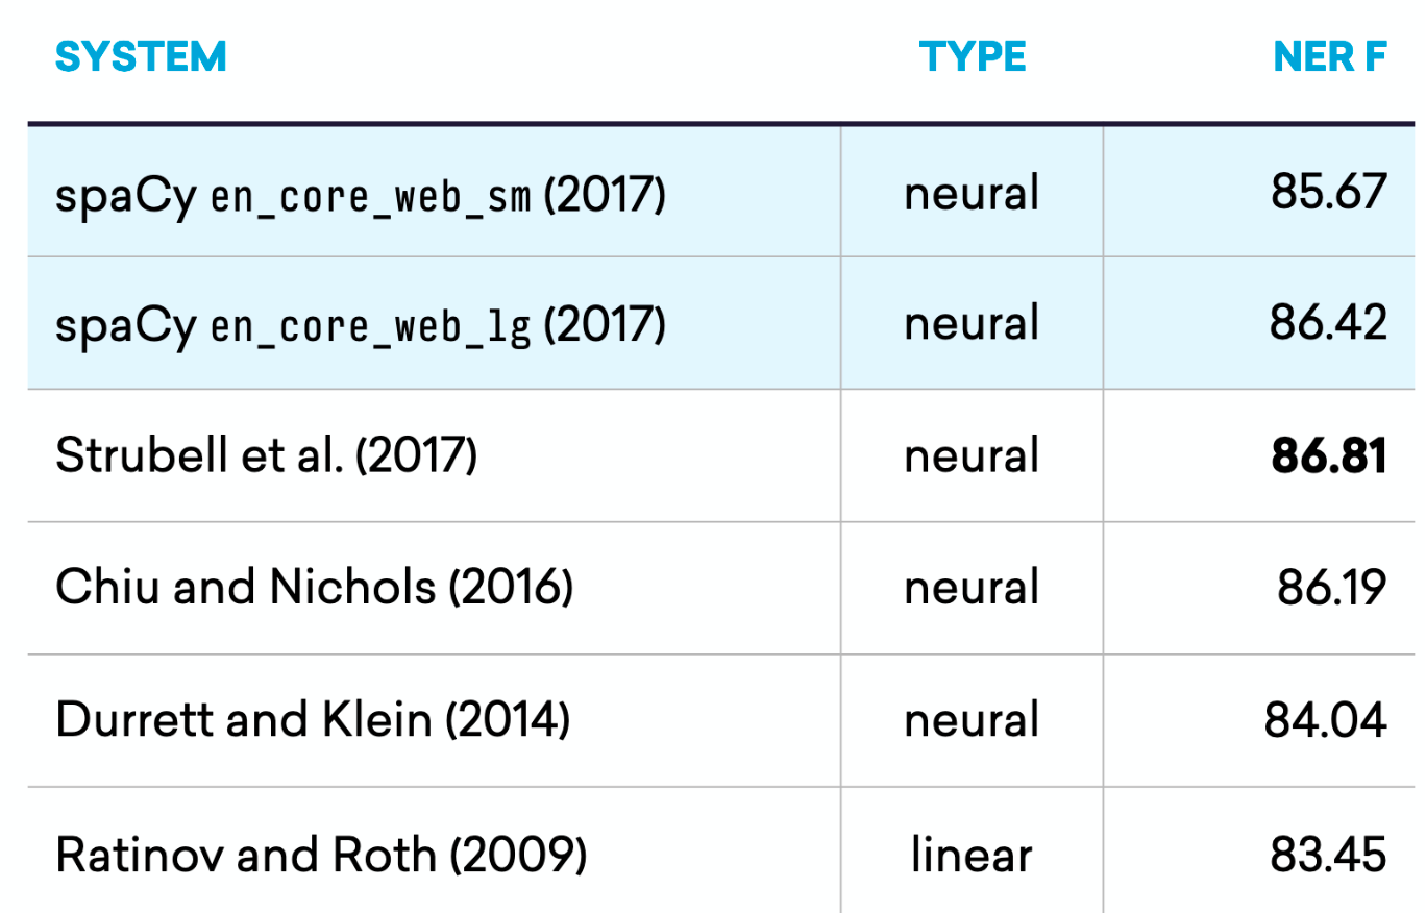
\includegraphics{assets/state-of-the-art_difficulties.pdf} 

}

\caption{Principales avances del estado del arte para NER en los últimos años.}\label{fig:spacy-algos}
\end{figure}

Las razones por las cuales esto ocurre escapa el alcance de este trabajo pero se pueden resumir bajo la ley de los rendimientos decrecientes (Case \& Fair, \protect\hyperlink{ref-lawOfDiminishingReturns}{1999}). Se necesita mucho esfuerzo académico para obtener una mejora marginal en el estado del arte actual.

Es por esto que resulta interesante analizar que otro tipo de problemas podemos abordar en este trabajo.

\hypertarget{dominios-del-problema}{%
\paragraph{Dominios del problema}\label{dominios-del-problema}}

Existe un hilo conductor en el que todas las investigaciones mencionadas en la figura \ref{fig:spacy-algos} coinciden; incluso los sistemas \emph{NER} más avanzadas son frágiles, dado que los sistemas NER desarrollados para un dominio no suelen comportarse bien en otros dominios (Poibeau \& Kosseim, \protect\hyperlink{ref-Poibeau2000ProperNE}{2000}). La puesta a punto de un sistema \emph{NER} para un nuevo dominio conlleva un esfuerzo considerable. Esto es cierto para modelos basados en reglas y para sistemas estadísticos.

Se entiende por dominio a todos los textos que en su conjunto forman un \emph{corpus} común. Ejemplos de estos son \enquote{Noticias periodísticas}, \enquote{Textos jurídicos}, \enquote{Reportes militares}, \enquote{Papers académicos}, etc.

\hypertarget{los-datos-son-el-problema}{%
\subsection{Los datos son el problema}\label{los-datos-son-el-problema}}

Por todo lo mencionado, es evidente que el cuello de botella para el avance de esta y muchas areas de la \enquote{Inteligencia Artificial} es el la captura de datos, no los algoritmos (Honnibal \& Montani, \protect\hyperlink{ref-montani_AI}{2016}).

En particular para el estado actual del arte de \emph{NER} es necesario tener el cuerpo de textos a analizar (\emph{corpus}) tagueado de tal manera que se conozcan previamente los nombres y tipos de entidades de un subconjunto de textos para inferir sobre el resto.

Este aprendizaje se carga en lo que se reconoce como un \enquote{Modelo estadístico} y es a ese modelo al que se le pide inferir nuevos resultados. En nuestra experiencia los modelos pre-entrenados de las diferentes plataformas / librerias / frameworks y trabajos académicos resultan siempre insuficientes para el uso en producción de los mismos.

De esta manera queda bien definido el problema que queremos atacar (y el título de este trabajo).

\begin{quote}
Creación eficiente de modelos estadísticos para detección automática y precisa de entidades nombradas.
\end{quote}

Para este fin se creó un sistema informático que permitirá obtener resultados a la altura de de las soluciones del estado del arte para cualquier \emph{corpus} de documentos que posea una cantidad suficiente de datos.

\newpage

\hypertarget{state-of-art}{%
\section{Estado del arte}\label{state-of-art}}

El análisis del estado del arte fue basado en la definición del problema.

\hypertarget{stack-de-software}{%
\subsection{Stack de software}\label{stack-de-software}}

\emph{Python} es el lenguaje más utilizado para resolver problemas de Machine Learning, en especial \emph{NLP} (Elliott, \protect\hyperlink{ref-github_machine_learning}{2019})

Spacy es el \emph{framework} mejor ranqueado para la tarea de \emph{NLP} (Elliott, \protect\hyperlink{ref-github_machine_learning}{2019}) y sabemos por la figura \ref{fig:spacy-algos} que obtiene resultados a-la-par del estado del arte actual.

Además la implementación de \emph{spaCy} es robusta y orientada a la creación de apliciones para producción, a diferencia de muchas otras librerías de \emph{NLP} que sólo se utilizan con fines académicos.

\hypertarget{el-pipeline}{%
\subsection{El pipeline}\label{el-pipeline}}

Todas las operaciones de analisis de lenguaje natural sobre textos no estructurados tienen como primer paso el de separar los mismos en tokens. Luego, el documento se procesa en varios pasos diferentes que consisten en el \enquote{pipeline de procesamiento}. Usualmente los pasos consisten en un etiquetador, un analizador sintáctico y un reconocedor de entidades en el caso de \emph{NER}.

Cada componente del pipeline mostrado en la figura \ref{fig:spacy-pipeline} devuelve el un documento \emph{Doc} procesado, que luego se pasa al siguiente componente.

\begin{figure}[H]

{\centering 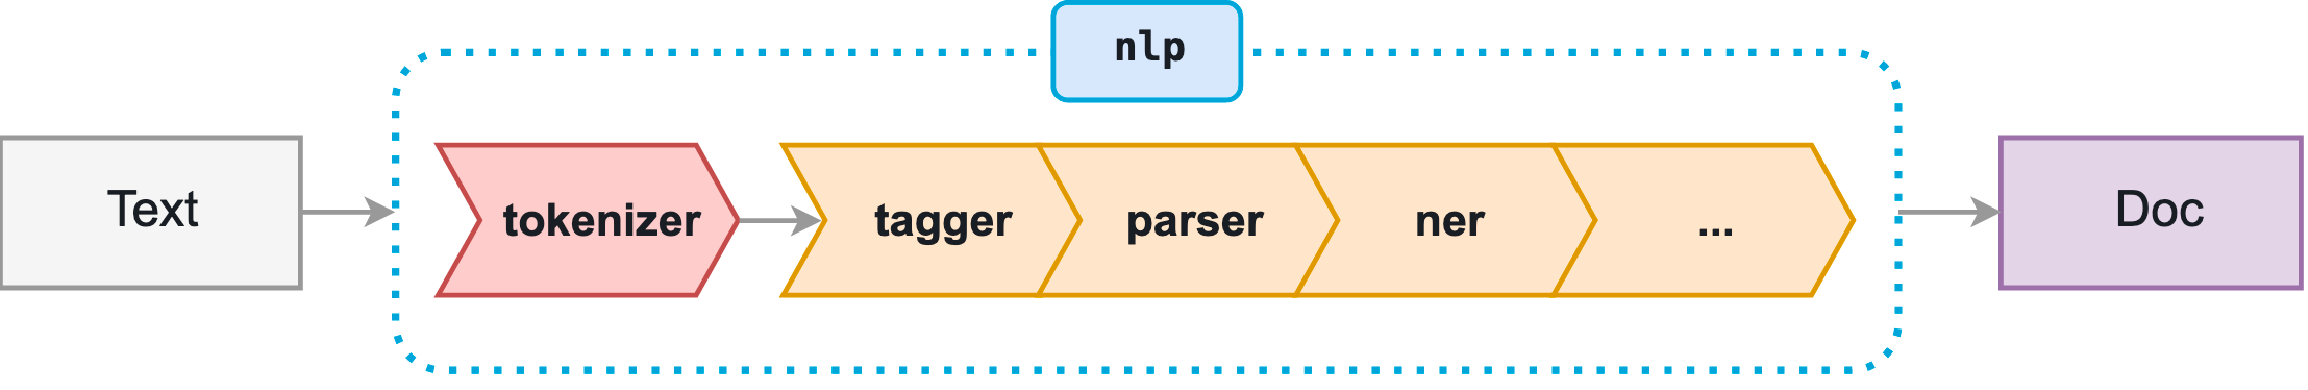
\includegraphics{assets/spacy_pipeline.pdf} 

}

\caption{Pipeline standard para los algoritmos de NER.}\label{fig:spacy-pipeline}
\end{figure}

En este capítulo estudiaremos la morfología de dicho pipeline.

\hypertarget{algoritmo-de-tokenizaciuxf3n}{%
\subsection{Algoritmo de tokenización}\label{algoritmo-de-tokenizaciuxf3n}}

Para tokenizar un texto de manera correcta no basta con separar el mismo en espacios. Dependiendo del lenguaje que se esté estudiando, existen excepciones a esta regla y otros caracteres que representan separaciones entre tokens segun el contexto de los mismos.

En particular, \emph{spaCy} posee un algoritmo de tokenización inteligente que puede ser resumido de la siguiente manera:

\begin{enumerate}
\def\labelenumi{\arabic{enumi}.}
\tightlist
\item
  Iterar sobre subcadenas separadas por espacios en blanco.
\item
  Comprobar si existe una regla definida explícitamente para esta subcadena. Si existe, usarla.
\item
  De lo contrario, intentar consumir un prefijo. Si consumimos un prefijo, regrese al punto \#2, para que los casos especiales siempre tengan prioridad.
\item
  Si no se puede consumir un prefijo, intente consumir un sufijo y luego regrese al punto \#2.
\item
  Si no se puede consumir un prefijo ni un sufijo, buscar un caso especial.
\item
  Buscar una coincidencia de token
\item
  Buscar \enquote{infijos} - cosas como guiones, etc. y dividir la subcadena en tokens en todos los infijos.
\item
  Una vez que no se pueda consumir más de la cadena, tratarla como un token único.
\end{enumerate}

Ejemplo:

\begin{figure}[H]

{\centering 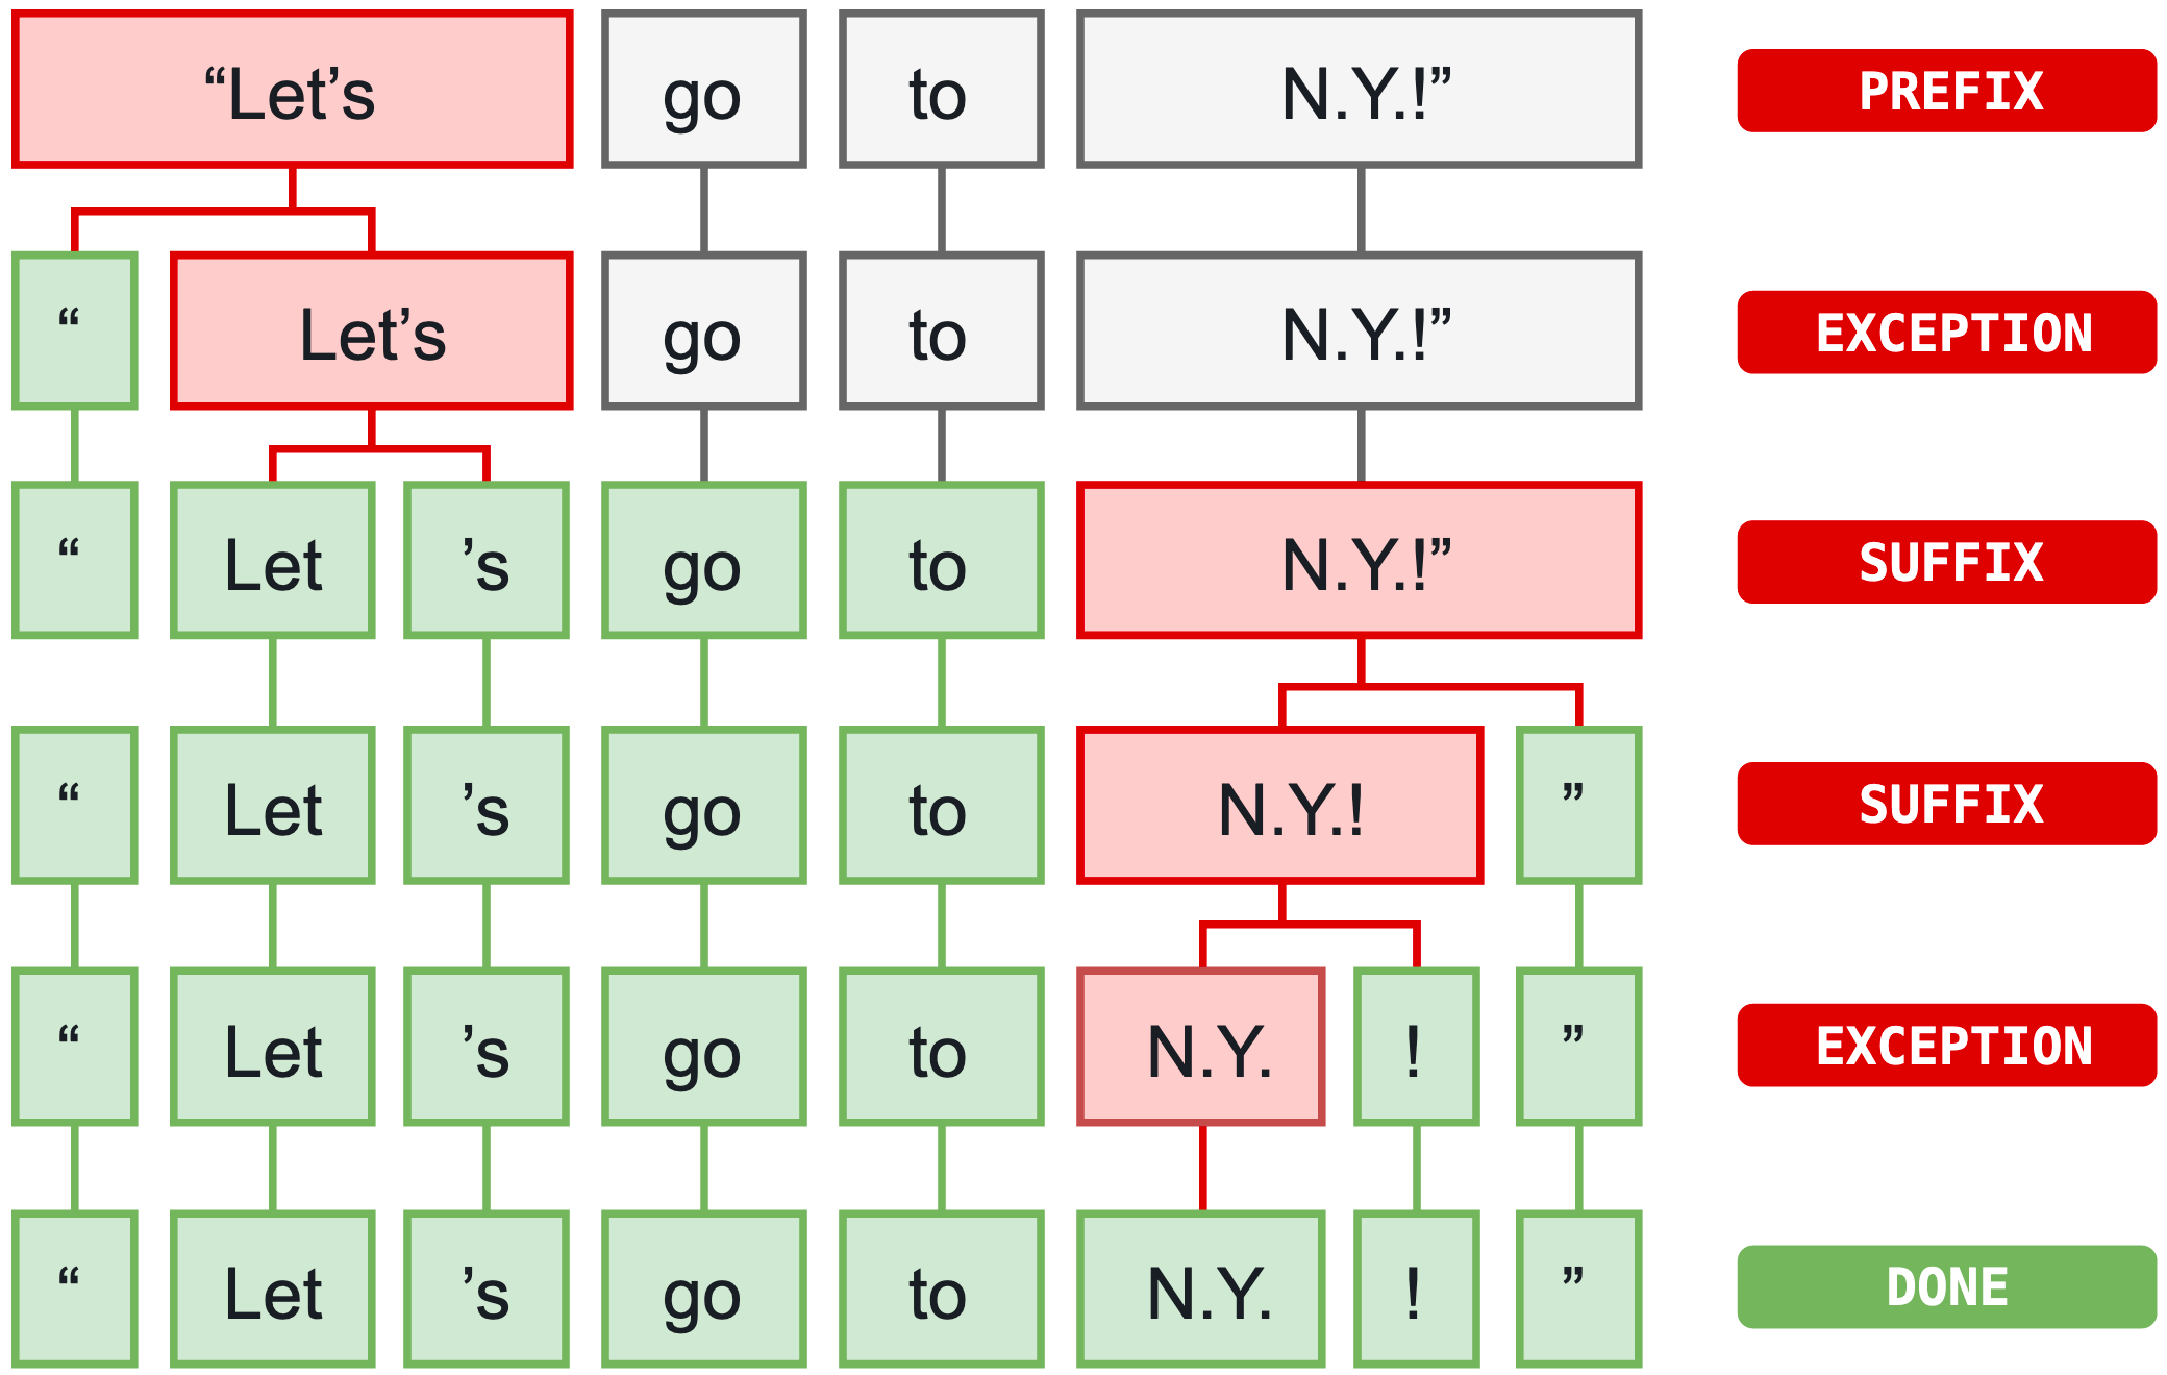
\includegraphics{assets/spacy_tokenization.pdf} 

}

\caption{Transiciones del modelo Stack-LSTM indicando la acción aplicada y el estado resultante.}\label{fig:spacy-tokenization}
\end{figure}

\hypertarget{modelos-basados-en-reglas}{%
\subsection{Modelos basados en reglas}\label{modelos-basados-en-reglas}}

Antes de entrar en detalles de cómo trabaja el modelo estadístico de spacy y entender sus fortalezas es importante esbozar brevemente el grupo de algorítmos más \enquote{naive} posible. El de los modelos basados en reglas fijas.

En estos modelos se implementan reglas finitas o expresiones regulares para la detección de las entidades. Las principales limitaciones de este enfoque son:

\begin{itemize}
\tightlist
\item
  \textbf{Mucho trabajo manua}l: el sistema \emph{Rule Based} exige un profundo conocimiento del dominio, este analisis debe ser realizado por humanos expertos en el dominio.
\item
  \textbf{Consumo de tiempo}: la generación de reglas para un sistema complejo es difícil y requiere mucho tiempo.
\item
  \textbf{Menor capacidad de aprendizaje}: el sistema generará el resultado según las reglas, por lo que la capacidad de aprendizaje del sistema por sí mismo es baja.
\item
  \textbf{Dominios complejos}: si el corpus demasiado complejo, la creación del sistema RB puede llevar mucho tiempo y análisis. La identificación de patrones complejos es una tarea desafiante en el enfoque RB.
\end{itemize}

\hypertarget{modelos-de-deep-learning}{%
\subsection{\texorpdfstring{Modelos de \enquote{\emph{deep-learning}}}{Modelos de ``deep-learning''}}\label{modelos-de-deep-learning}}

Cuando se busca mejorar el aprendizaje automático, generalmente se piensa en la eficiencia y la precisión, pero la dimensión más importante es la generalidad. Este es el modelo estadístico que usa \emph{spaCy}.

La mayoría de los problemas de \texttt{NLP} pueden reducirse a problemas de aprendizaje automático que toman uno o más textos como entrada. Si podemos transformar estos textos en vectores, podemos reutilizar soluciones de aprendizaje profundo (\emph{deep-learning}) de propósito general.

Las representaciones de palabras embebidas (\emph{embebed-words}), también conocidas como \enquote{vectores de palabras} (\emph{word-vectors}), son una de las tecnologías de procesamiento de lenguaje natural más utilizadas en el estado del arte actual. El modelo de \emph{deep learning} utilizado por \emph{spaCy} puede ser descripto en cuatro pasos.

Los \emph{word-embeddings} permiten tratar a las palabras individuales como \enquote{unidades de significado}, en lugar de identificaciones completamente distintas. A este proceso se le conoce como \textbf{\emph{embed}}.

Sin embargo, la mayoría de los problemas de \emph{NLP} requieren la comprensión de tramos de texto más largos, no solo palabras individuales. Al juntar un conjunto de \emph{word-embeddings} en una secuencia de vectores, se usan RNN bidireccionales para codificar los vectores en una matriz de oración. Las filas de esta matriz pueden entenderse como \enquote{vectores-de-tokens}: son sensibles al contexto del token dentro de la oración. Este paso se lo llama \textbf{\emph{encode}}.

Finalmente, el mecanismo de \textbf{\emph{attend}} le permite reducir la matriz de oración a un vector de oración, listo para la predicción (\textbf{\emph{predict}}).

De esta manera quedan definidas las piezas que describen al modelo de \emph{spaCy}:

\begin{figure}[H]

{\centering 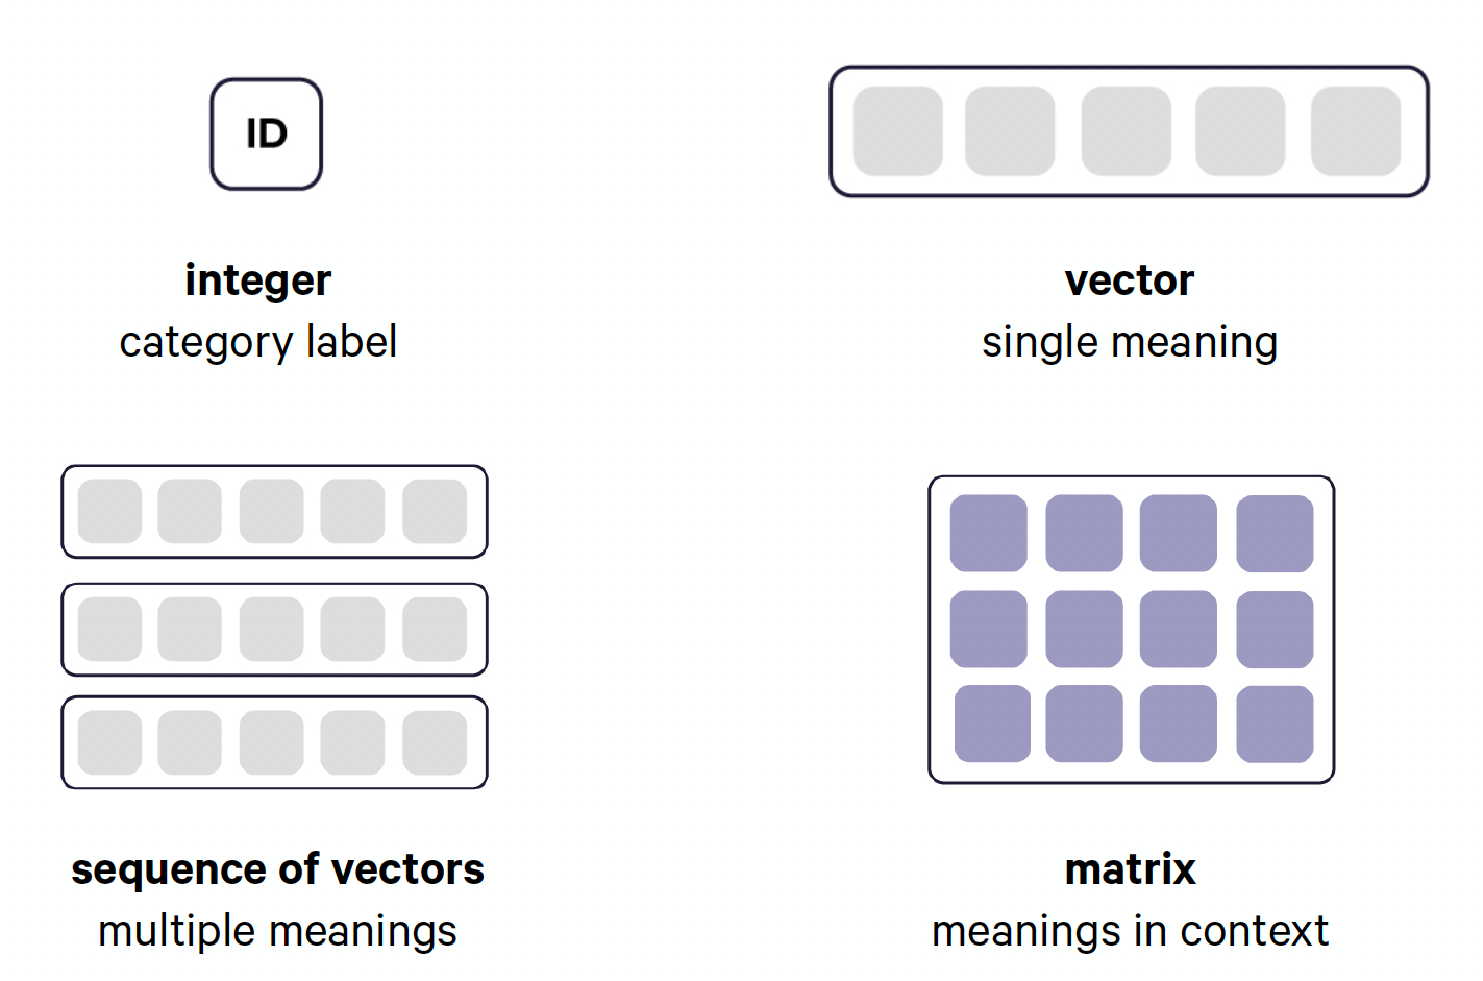
\includegraphics{assets/deep-learning-formula-nlp_shapes.pdf} 

}

\caption{Estados posibles para las diferentes etapas de la CNN.}\label{fig:formula-shapes}
\end{figure}

Estos 4 procesos seran descriptos en detalle en las siguientes secciones.

\hypertarget{embed}{%
\subsubsection{\texorpdfstring{\emph{Embed}}{Embed}}\label{embed}}

\begin{quote}
Resuelve el problema: \enquote{todas las palabras se ven iguales para la computadora}
\end{quote}

La idea de \emph{word embeddings} es la de \enquote{embeber} el conjunto de tokens que componen términos con información adicional. El resultado de esta operación es una estructura abstracta que puede ser descripta como un \enquote{vector de significado}.

\begin{figure}[H]

{\centering 
\includegraphics{assets/deep-learning-formula-nlp_embed.pdf} 

}

\caption{Embed.}\label{fig:formula-embed}
\end{figure}

Es importante destacar que en la etapa de \emph{embed}, toda la información de significado es principalmente independiente del contexto en el cual esta siendo utilizada y por esta razón es facilmente obtenible del corpus no tagueado de datos (los algoritmos pueden darse cuenta de que palabras están relacionadas entre sí de manera eficiente y no supervisada).

Esto permite al modelo poder inferir significado a partir de la información no etiquetada dentro del problema en particular a resolver (el de \emph{NER}).

Una tabla de \emph{word-embeddings} mapea vectores largos binarios y esparsos en vectores cortos densos y continuos, cargados de significado relevante. Existen varias estrategias para enriquecer los \emph{tokens} con información adicional. Las dos fuentes más grandes de información embebida son las de \textbf{información lingüística} y los \textbf{\emph{word-vectors}}.

\hypertarget{informaciuxf3n-liguxfcuxedstica}{%
\paragraph{Información ligüística}\label{informaciuxf3n-liguxfcuxedstica}}

El objetivo de ésta etapa es la de encontrar las características intrínsecas de cada palabra. Las principales características lingüísticas detectadas están resumidas en el siguiente ejemplo.

\begin{figure}[H]

{\centering 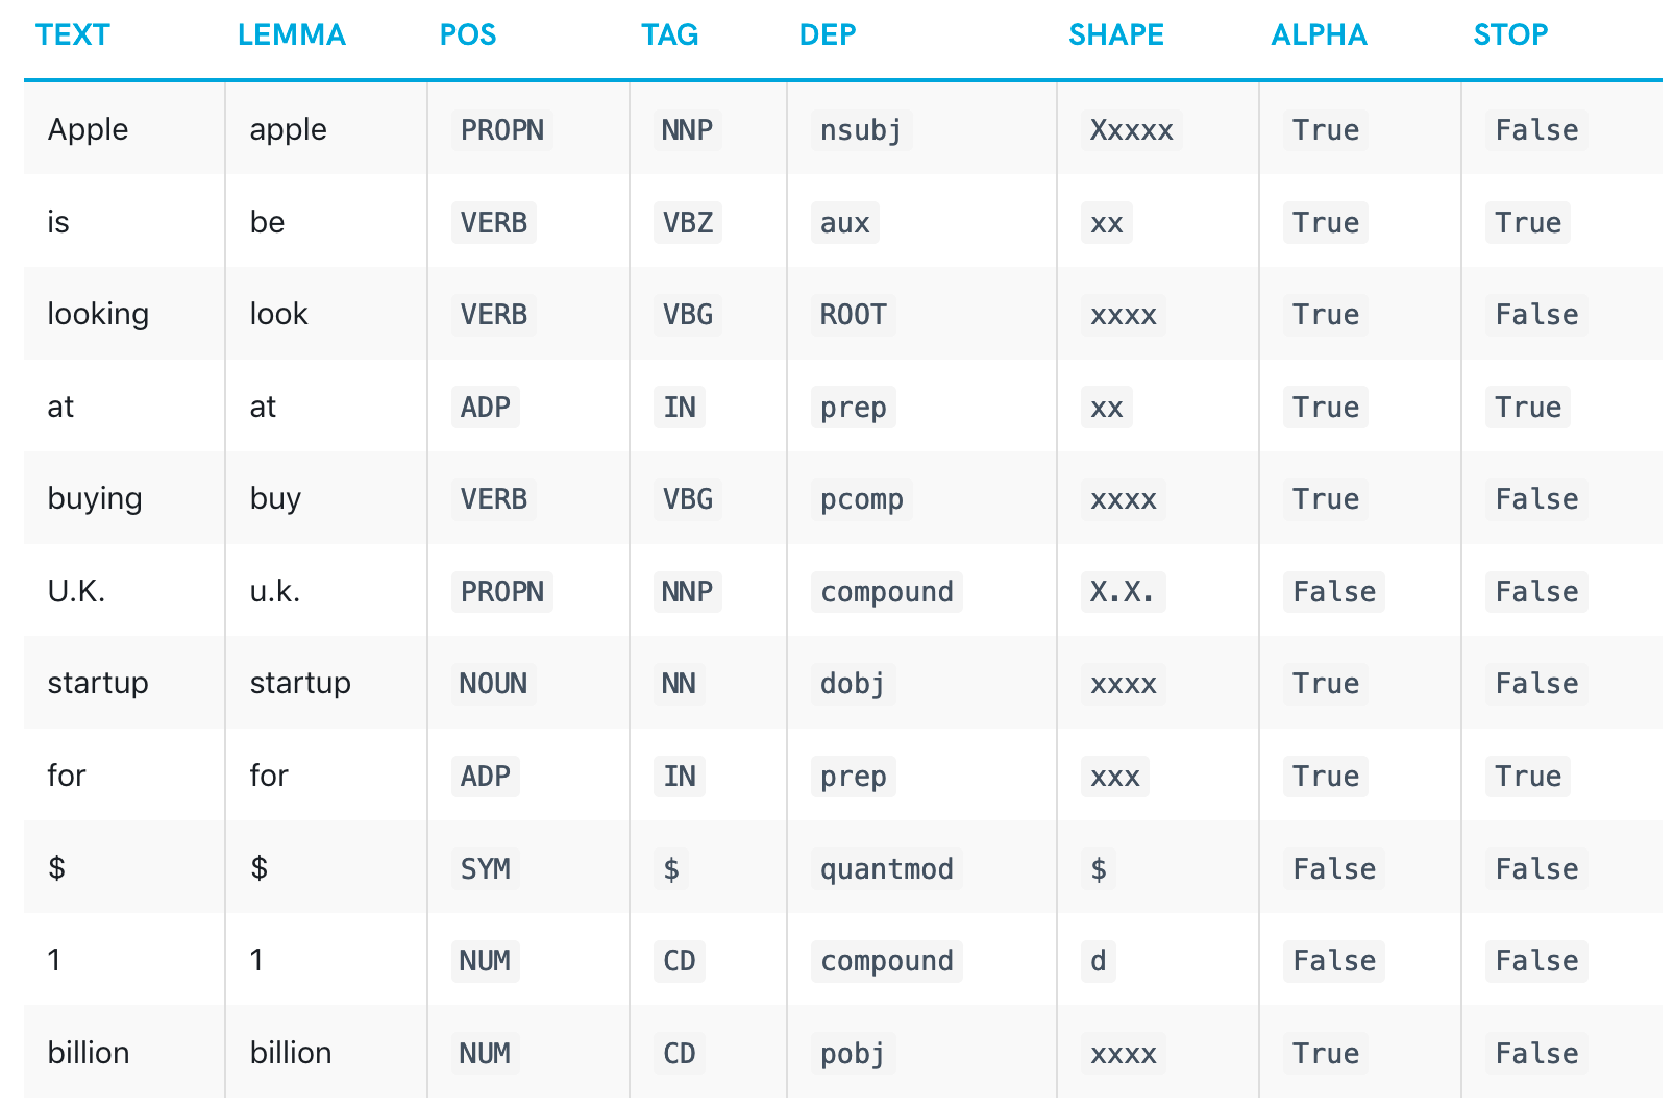
\includegraphics{assets/pos.pdf} 

}

\caption{Características lingüísticas.}\label{fig:formula-pos}
\end{figure}

\begin{itemize}
\tightlist
\item
  \textbf{Text}: la palabra original texto.
\item
  \textbf{Lemma}: La forma básica de la palabra. \texttt{Es\ -\textgreater{}\ ser}. Esto permite a las siguientes etapas trabajar con una definicón canónica del token.
\item
  \textbf{POS}: la etiqueta simple de parte-del-discurso (POS).
\item
  \textbf{Tag}: la etiqueta detallada de parte del discurso (POS).
\item
  \textbf{Dep}: dependencia sintáctica, es decir, la relación entre tokens.
\item
  \textbf{Shape}: la forma de la palabra: mayúsculas, puntuación, dígitos. Muy útil para detectar patrones como números telefónicos, documentos de identidad, CBUs, etc.
\item
  \textbf{is alpha}: ¿el token es una secuencia de caracteres alfabéticos?
\item
  \textbf{is stop} : ¿es el token parte de una lista de \enquote{palabras de \emph{stop}}, es decir, las palabras más comunes del idioma?
\end{itemize}

\hypertarget{word-vectors}{%
\subparagraph{\texorpdfstring{\emph{Word Vectors}}{Word Vectors}}\label{word-vectors}}

A diferencia de la información lingüística que es obtenida en el momento, existen otros tipos de \emph{embeddings} más poderosos que son los productos de pre-entrenamientos; como el caso de los \emph{word-vectors}. Los mismos se generan mediante la concatenación de atributos léxicos como \emph{NORM}, \emph{PREFIX}, \emph{SUFFIX} y \emph{SHAPE}. Luego se usa una capa oculta de una red neuronal convolucional (\emph{CNN}) para permitir una combinación no lineal de la información en estos vectores concatenados.

Los \emph{word-vectors} son particularmente útiles para términos que no están bien representados en los datos de entrenamiento etiquetados. En nuestro uso de reconocimiento de entidades, no siempre habrá suficientes ocurrencias. Por ejemplo, en los datos de entrenamiento es posible que existan ocurrencias del término \enquote{Coca-Cola}, pero ninguna del término \enquote{Manaos}.
Es interesante pensar a las palabras como \enquote{vectores de significado}. Dentro del espacio vectorial de significados el vector \enquote{perro} se encuentra cercano al de \enquote{cachorro}, \enquote{beagle}, \enquote{bulldog}, \enquote{poodle}. Esto permite al modelo poder inferir nuevas relaciones en base a una cantidad reducida de entradas.
Los \emph{word-vectors} ponen ese hecho a disposición del modelo de reconocimiento de entidades. Si bien no existen ejemplos de \enquote{Manaos} etiquetados como \enquote{Producto}; se verá que \enquote{Manaos} tiene un vector de palabras que generalmente corresponde a los términos de un producto, por lo que puede hacer la inferencia. Y si se quiere, se puede llegar incluso al detalle de que es una \enquote{Gaseosa}.

Otra forma interesante de analizar y entender los \emph{word-vectors} en su contexto de espacio vectorial multidimensional de significados es a través del algebra de vectores, como se muestra en el trabajo \enquote{\emph{Towards Understanding Linear Word Analogies}} (Ethayarajh, Duvenaud, \& Hirst, \protect\hyperlink{ref-ethayarajh-etal-2019-towards}{2019}):

\begin{figure}[H]

{\centering 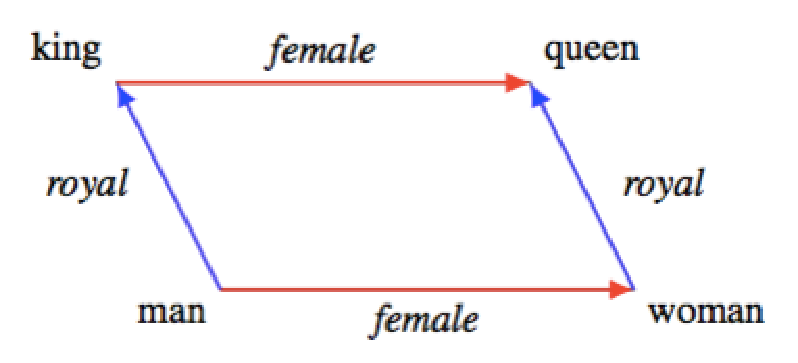
\includegraphics[width=0.6\linewidth]{assets/parallelogram.pdf} 

}

\caption{Parallelogram structure in the vector space (by definition).}\label{fig:vec-parallelogram}
\end{figure}

Es facil de entender viendo la figura \ref{fig:vec-parallelogram} que al realizar algebra entre los diferentes vectores de significado se pueden inferir nuevos conceptos:

\[\vec{Rey} - \vec{Hombre} \approx \vec{Realeza}\]
\[\vec{Rey} - \vec{Hombre} + \vec{Mujer} \approx \vec{Reina}\]

\hypertarget{encode}{%
\subsubsection{\texorpdfstring{\emph{Encode}}{Encode}}\label{encode}}

\begin{quote}
Resuelve el problema: el contexto de los significados es relevante y esta siendo descartado,
\end{quote}

El resultado de esta etapa es la de codificar vectores \textbf{independientes-de-contexto} en matrices de oración \textbf{sensibles-al-contexto}.

\begin{figure}[H]

{\centering 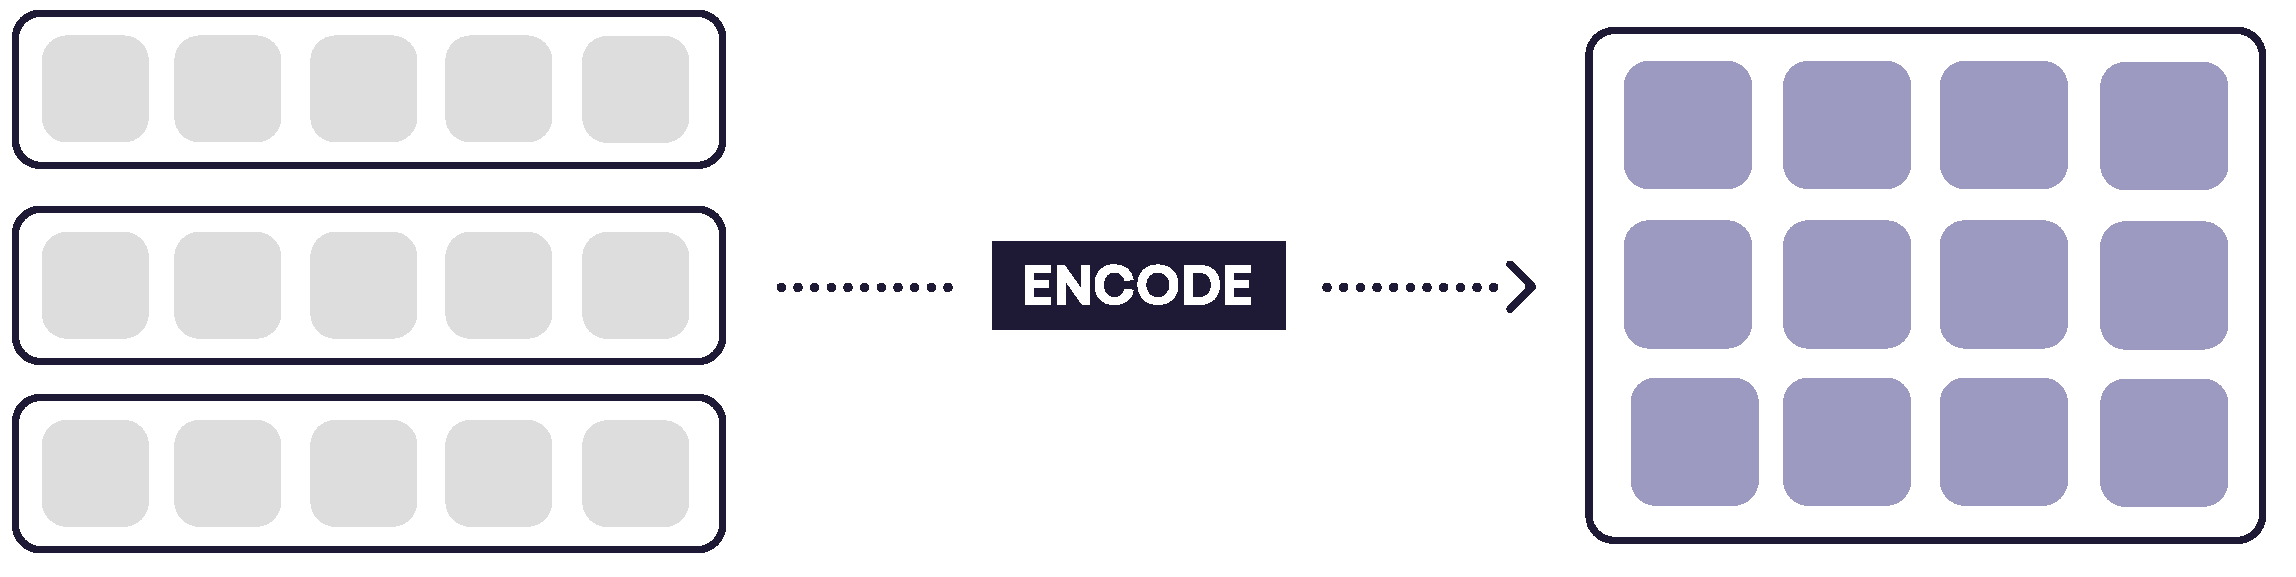
\includegraphics{assets/deep-learning-formula-nlp_encode.pdf} 

}

\caption{Encode.}\label{fig:formula-encode}
\end{figure}

La tecnología utilizada para esta etapa es una Red Neuronal Convolucional en la que la oración es analizada como una \emph{moving window} de tres vectores en la que cada vector analiza su significado en relación con un vector previo y un vector posterior. Es decir, cada vector se estudia dentro del contexto de los dos vectores que lo rodean. Luego los vectores subsiguientes se evaluan de igual manera, por lo que se genera naturalmente un \enquote{efecto de decaimiento} en el que el contexto de los vectores más lejanos tiene una relevancia cada vez menor.

\hypertarget{attend}{%
\subsubsection{\texorpdfstring{\emph{Attend}}{Attend}}\label{attend}}

\begin{quote}
Resuelve el problema: tenemos demasiada información para inferir un significado específico al problema a resolver.
\end{quote}

En esta etapa toda la información generada en las etapas anteriores es analizada a través de un vector de entrada o tambien conocido como \enquote{vector de consulta} o \enquote{vector de contexto} representado en la figura \ref{fig:formula-attend} como un vector mas oscuro.

\begin{figure}[H]

{\centering 
\includegraphics{assets/deep-learning-formula-nlp_attend.pdf} 

}

\caption{Attend.}\label{fig:formula-attend}
\end{figure}

Al reducir la matriz a un vector, necesariamente se está perdiendo información. Es por eso que el \enquote{vector de contexto} es crucial: Indica que información descartar, de modo que el \enquote{vector resumen} se adapte a la red que lo consume.

El análisis de estas estrategias de consulta escapa el alcance de este trabajo pero resulta un tema interesante de investigación en sí mismo. Por ejemplo, investigaciones recientes han demostrado que el mecanismo de atención es una técnica flexible y que se pueden usar nuevas variaciones para crear soluciones elegantes y poderosas. Por ejemplo, en el estudio de Ankur Parikh et al (Parikh, Täckström, Das, \& Uszkoreit, \protect\hyperlink{ref-parikh-etal-2016-decomposable}{2016}) presentan un mecanismo de atención que toma dos matrices de oraciones y genera un solo vector.

\hypertarget{predict}{%
\subsubsection{\texorpdfstring{\emph{Predict}}{Predict}}\label{predict}}

\begin{quote}
Resuelve el problema: necesito un valor específico y no una representación genérica abstracta.
\end{quote}

Finalmente en esta etapa tenemos un nuevo \enquote{vector de significado} que resulta de la consulta a la etapa anterior. Es necesario ahora traducir este vector a un \emph{token} efectivo. En el caso de \emph{NER}, el \emph{token} que interesa obtener es el de la etiqueta de entidad.

\begin{figure}[H]

{\centering 
\includegraphics{assets/deep-learning-formula-nlp_predict.pdf} 

}

\caption{Predict.}\label{fig:formula-predict}
\end{figure}

\hypertarget{use-of-cnn}{%
\subsection{Uso del modelo estadístico}\label{use-of-cnn}}

Experimentos en inglés, holandés, alemán y español muestran que se pueden obtener resultados a-la-par del estado del arte mediante el uso de un \enquote{autómata finito determinístico de pila} en conjunto con una red neuronal (Lample, Ballesteros, Subramanian, Kawakami, \& Dyer, \protect\hyperlink{ref-DBLP:journalsux2fcorrux2fLampleBSKD16}{2016}).

Este autómata de pila es el nexo entre la Red Neuronal Convolucional (\emph{CNN}) que contiene el modelo estadístico para predecir entidades en el texto completo. En el mismo, se envían cada uno de los estados porl los que se mueve para ir generando entidades con una herística del tipo \emph{greedy}.

La figura \ref{fig:lampe-1} muestra las posibles acciones de transición de este autómata.

\begin{itemize}
\tightlist
\item
  SHIFT: consume una token del input y al mueve al stack para generar una nueva entidad.
\item
  REDUCE: mueve el stack actual al output tagueado como entity.
\item
  OUT: consume una token del input y la mueve sl output directamente.
\end{itemize}

\begin{figure}[H]

{\centering 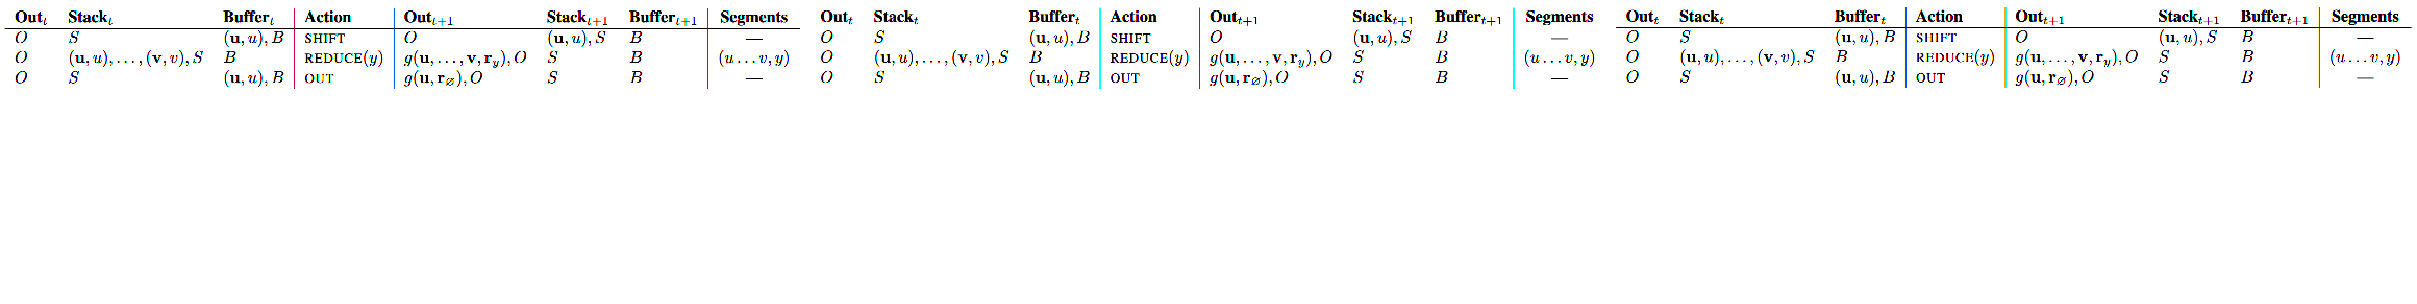
\includegraphics{assets/lampe_1.pdf} 

}

\caption{Transiciones del modelo Stack-LSTM indicando la acción aplicada y el estado resultante.}\label{fig:lampe-1}
\end{figure}

Para saber que acción tomar se consulta el modelo estadístico. En la figura \ref{fig:lampe-2} se puede ver un ejemplo de como se recorre una oración bajo el stack propuesto:

\begin{figure}[H]

{\centering 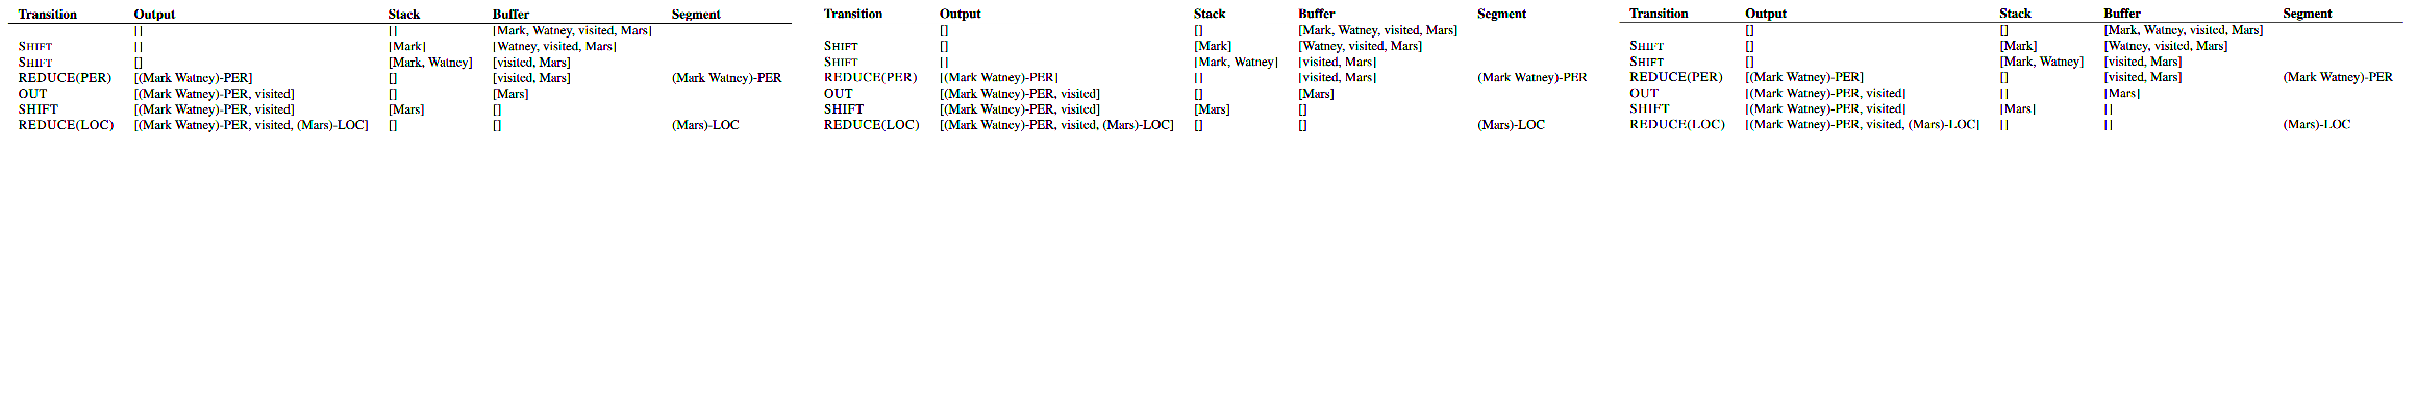
\includegraphics{assets/lampe_2.pdf} 

}

\caption{Secuencia de tranciciones para el ejemplo "Mark Watney visited Mars" en el modelo de Stack-LSTM.}\label{fig:lampe-2}
\end{figure}

\begin{itemize}
\tightlist
\item
  Primero se empieza con un stack vacío.
\item
  Se consume \emph{\enquote{Mark}} y la \emph{CNN} predice que es una posible Persona. Lo envia al stack.
\item
  Se consume \emph{\enquote{Watney}} y la \emph{CNN} predice que es una posible continuación de Persona. Lo envia al stack.
\item
  Se consume \emph{\enquote{visited}} y la \emph{CNN} predice que esto no forma parte de una entidad. Por lo tanto antes se \emph{REDUCE} la entidad \emph{\enquote{Mark Watney}} del stack actual.
\item
  Análogamente se detecta la entidad \emph{\enquote{Mars}}
\end{itemize}

La predicción que realiza la \emph{CNN} tiene un puntaje de 0 a 1; un porcentaje de certeza de que la token sea de un tipo específico. A veces las tokens pueden tener más de una etiqueta candidata a ser utilizada y éste es el método para desempatar este conflicto. Cuanto más cercano a \(0.5\) es ese punaje mayor es la incerteza.

\newpage

\hypertarget{implementation}{%
\section{NERd (Implementación)}\label{implementation}}

Definido el problema, queda claro que la creación de un modelo entrenado es de vital importancia para cualquier problema de etiquetado de entidades.
Es por ello que en el presente proyecto final hemos creado una herramienta para el entrenamiento eficiente de modelos estadísticos así como también una interfaz y API para poder consultar entidades.
El nombre de esta herramienta es \textbf{NERd}, sigla cuyo significado en inglés es \emph{\textbf{N}amed \textbf{E}ntity \textbf{R}ecognition \textbf{D}uh}\footnote{Expresión de obviedad. \emph{Used to express your belief that what was said was extremely obvious} (``Duh definition,'' \protect\hyperlink{ref-cambridge_duh}{2019})}!

Para organizar este capítulo vamos a realizar una descripción basada en el modelo de vistas de arquitectura 4+1 (Figura \ref{fig:arq41}).

\begin{figure}[H]

{\centering 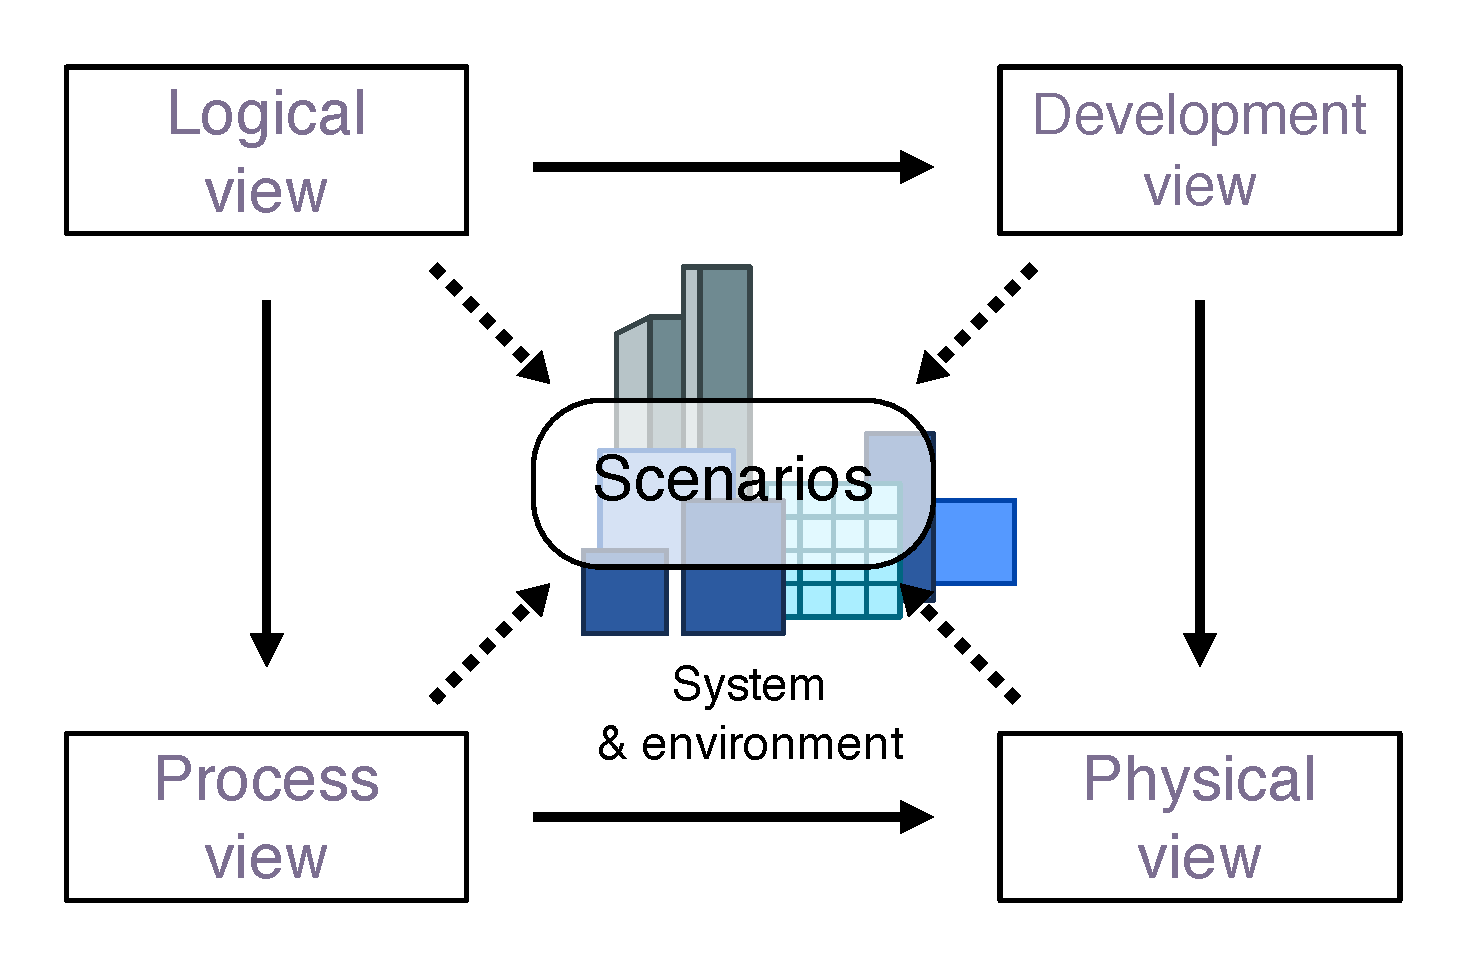
\includegraphics{assets/4+1_Architectural_View_Model.pdf} 

}

\caption{Ilustración de arquitectura 4+1.}\label{fig:arq41}
\end{figure}

Este modelo nos permite describir la aplicación de una manera genérica y ordenada.

\begin{quote}
\emph{The \enquote{4+1} view model is rather \enquote{generic}: other notations and tools can be used, other design methods can be used, especially for the logical and process decompositions, but we have indicated the ones we have used with success.}

\hfill --- (Kruchten, \protect\hyperlink{ref-Kruchten:1995:VMA:624610.625529}{1995})
\end{quote}

\hypertarget{vista-luxf3gica}{%
\subsection{Vista lógica}\label{vista-luxf3gica}}

\begin{quote}
La vista lógica se refiere a la funcionalidad que el sistema proporciona a los usuarios finales.
\end{quote}

A continuación detallamos distintas partes del servicio NERd así como también de la interfaz de entrenamiento.

\hypertarget{web}{%
\subsubsection{Web}\label{web}}

La página \emph{web} de \emph{NERd} está enfocada en las tareas de mantenimiento de los servicios ofrecidos por el \emph{API} así como también ofrece de interfaces que permiten a usuarios del sistema corregir de manera eficiente el modelo de inferencia.

\hypertarget{inicio}{%
\paragraph{Inicio}\label{inicio}}

La pantalla de inicio es donde se encuentran los accesos rápidos para entrenar el modelo o para buscar entidades en textos.
También se encuentra aquí una lista de los 5 usuarios que más contribuyeron a entrenar el modelo. Detrás de esta funcionalidad se busca generar un espíritu competitivo entre los usuarios para que los mismos busquen contribuir más (Figura \ref{fig:logic-home}). A este tipo de técnicas se las denomina \emph{gamification}.

\begin{figure}[H]

{\centering 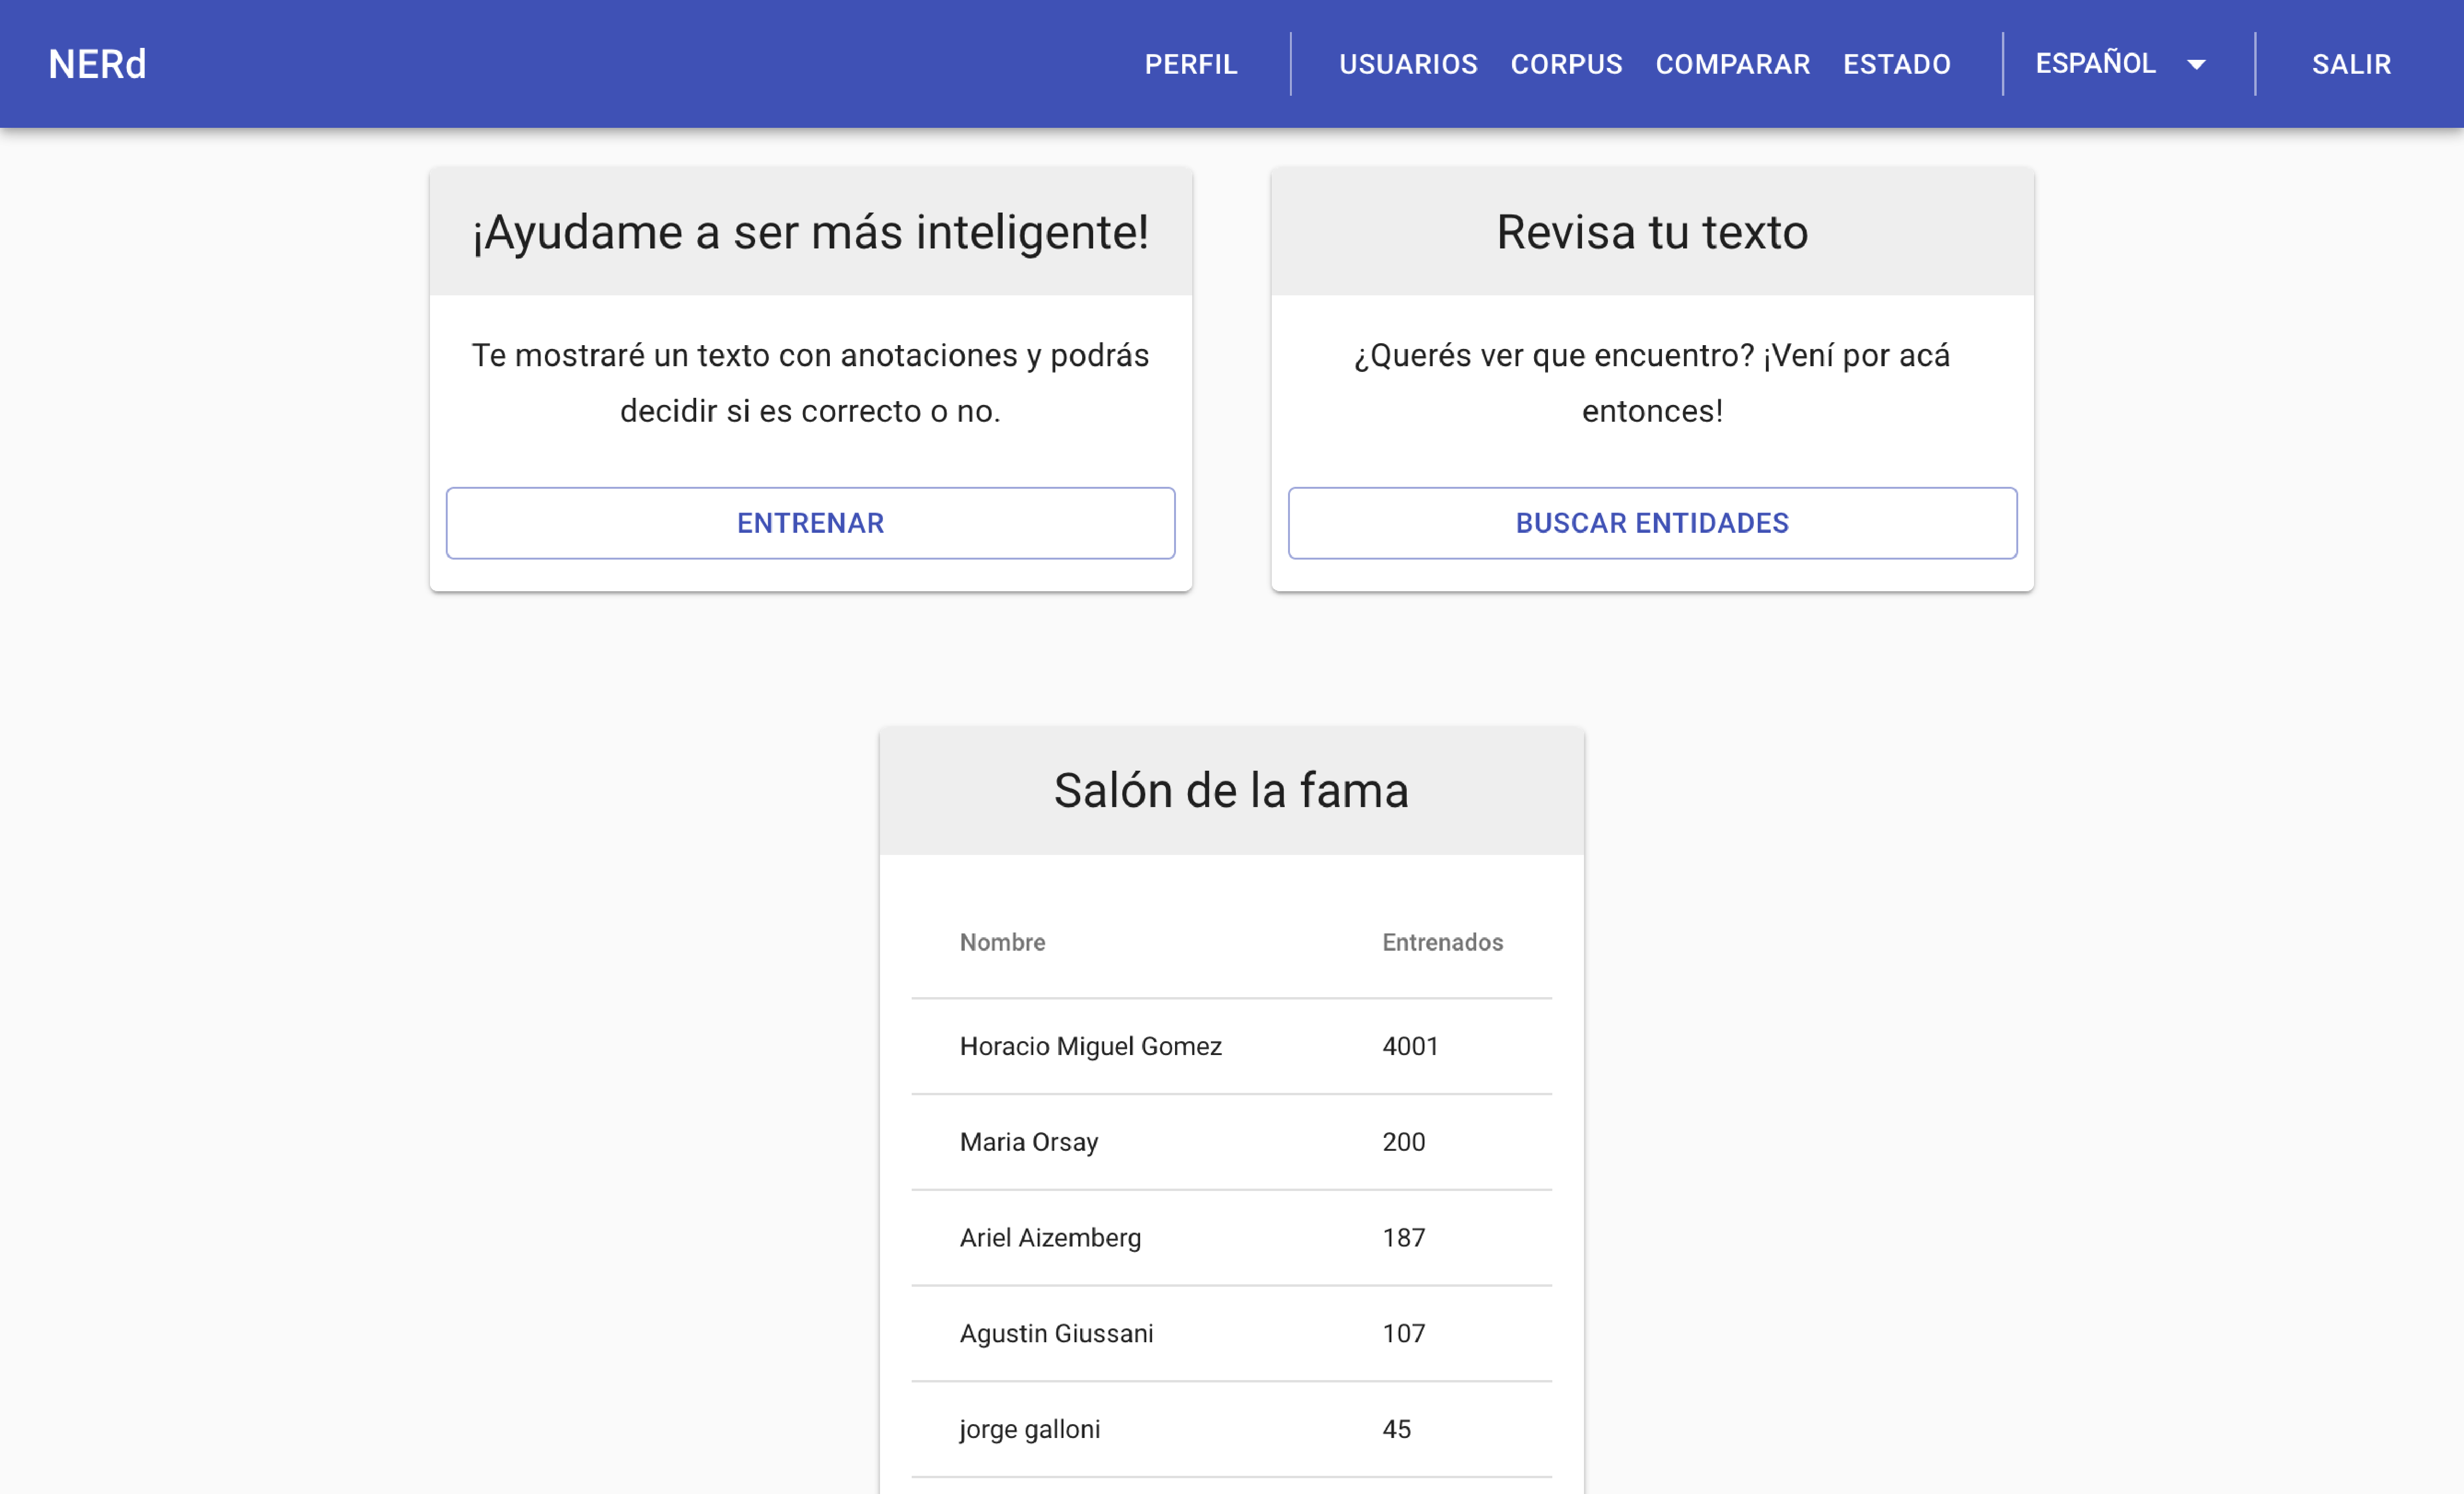
\includegraphics{assets/logic/home-logged-all.pdf} 

}

\caption{Pantalla de inicio con usuario logueado.}\label{fig:logic-home}
\end{figure}

Si la persona no cuenta con permisos de entrenador, se le sugiere que contacte a un administrador para que le otorgue el permiso (Figura \ref{fig:logic-home-logged-nontrainer}).

\begin{figure}[H]

{\centering 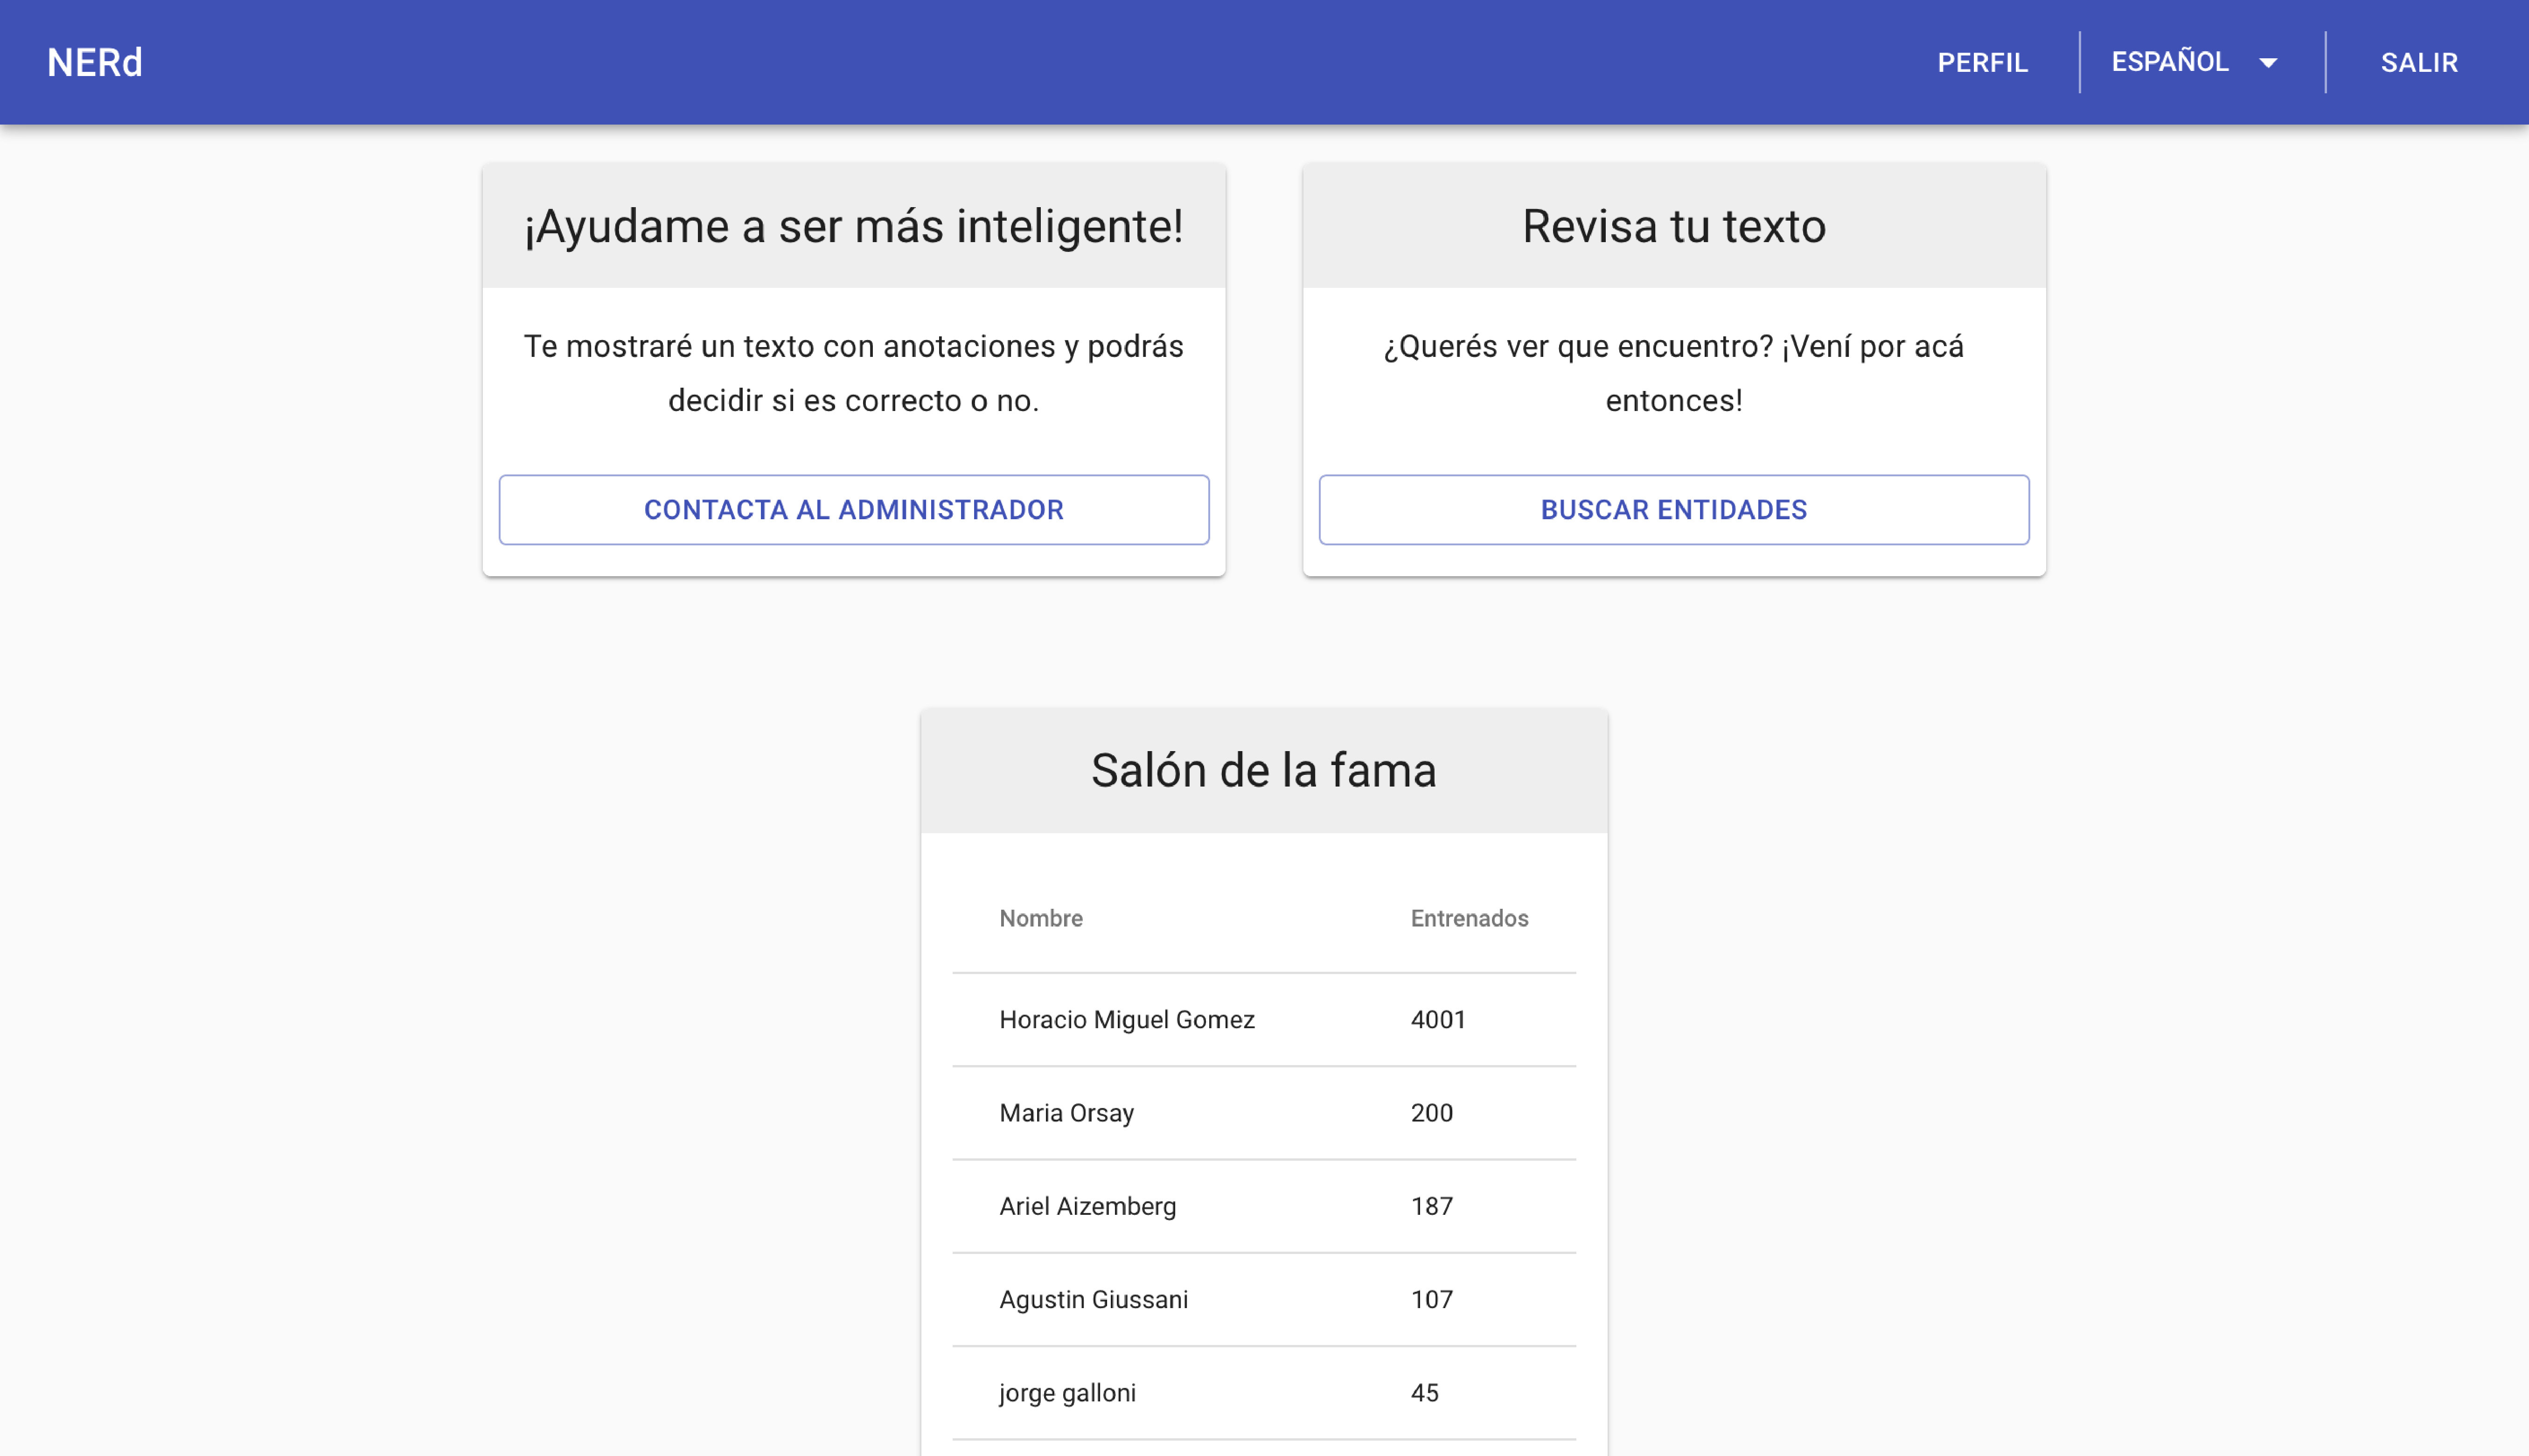
\includegraphics{assets/logic/home-logged-not_trainer.pdf} 

}

\caption{Pantalla de inicio sin rol de entrenador.}\label{fig:logic-home-logged-nontrainer}
\end{figure}

Si la persona visitando la página no cuenta con una sesión activa, se le invita a ingresar con una cuenta pre-existente o a registrarse (Figura \ref{fig:logic-home-anonymous}).

\begin{figure}[H]

{\centering 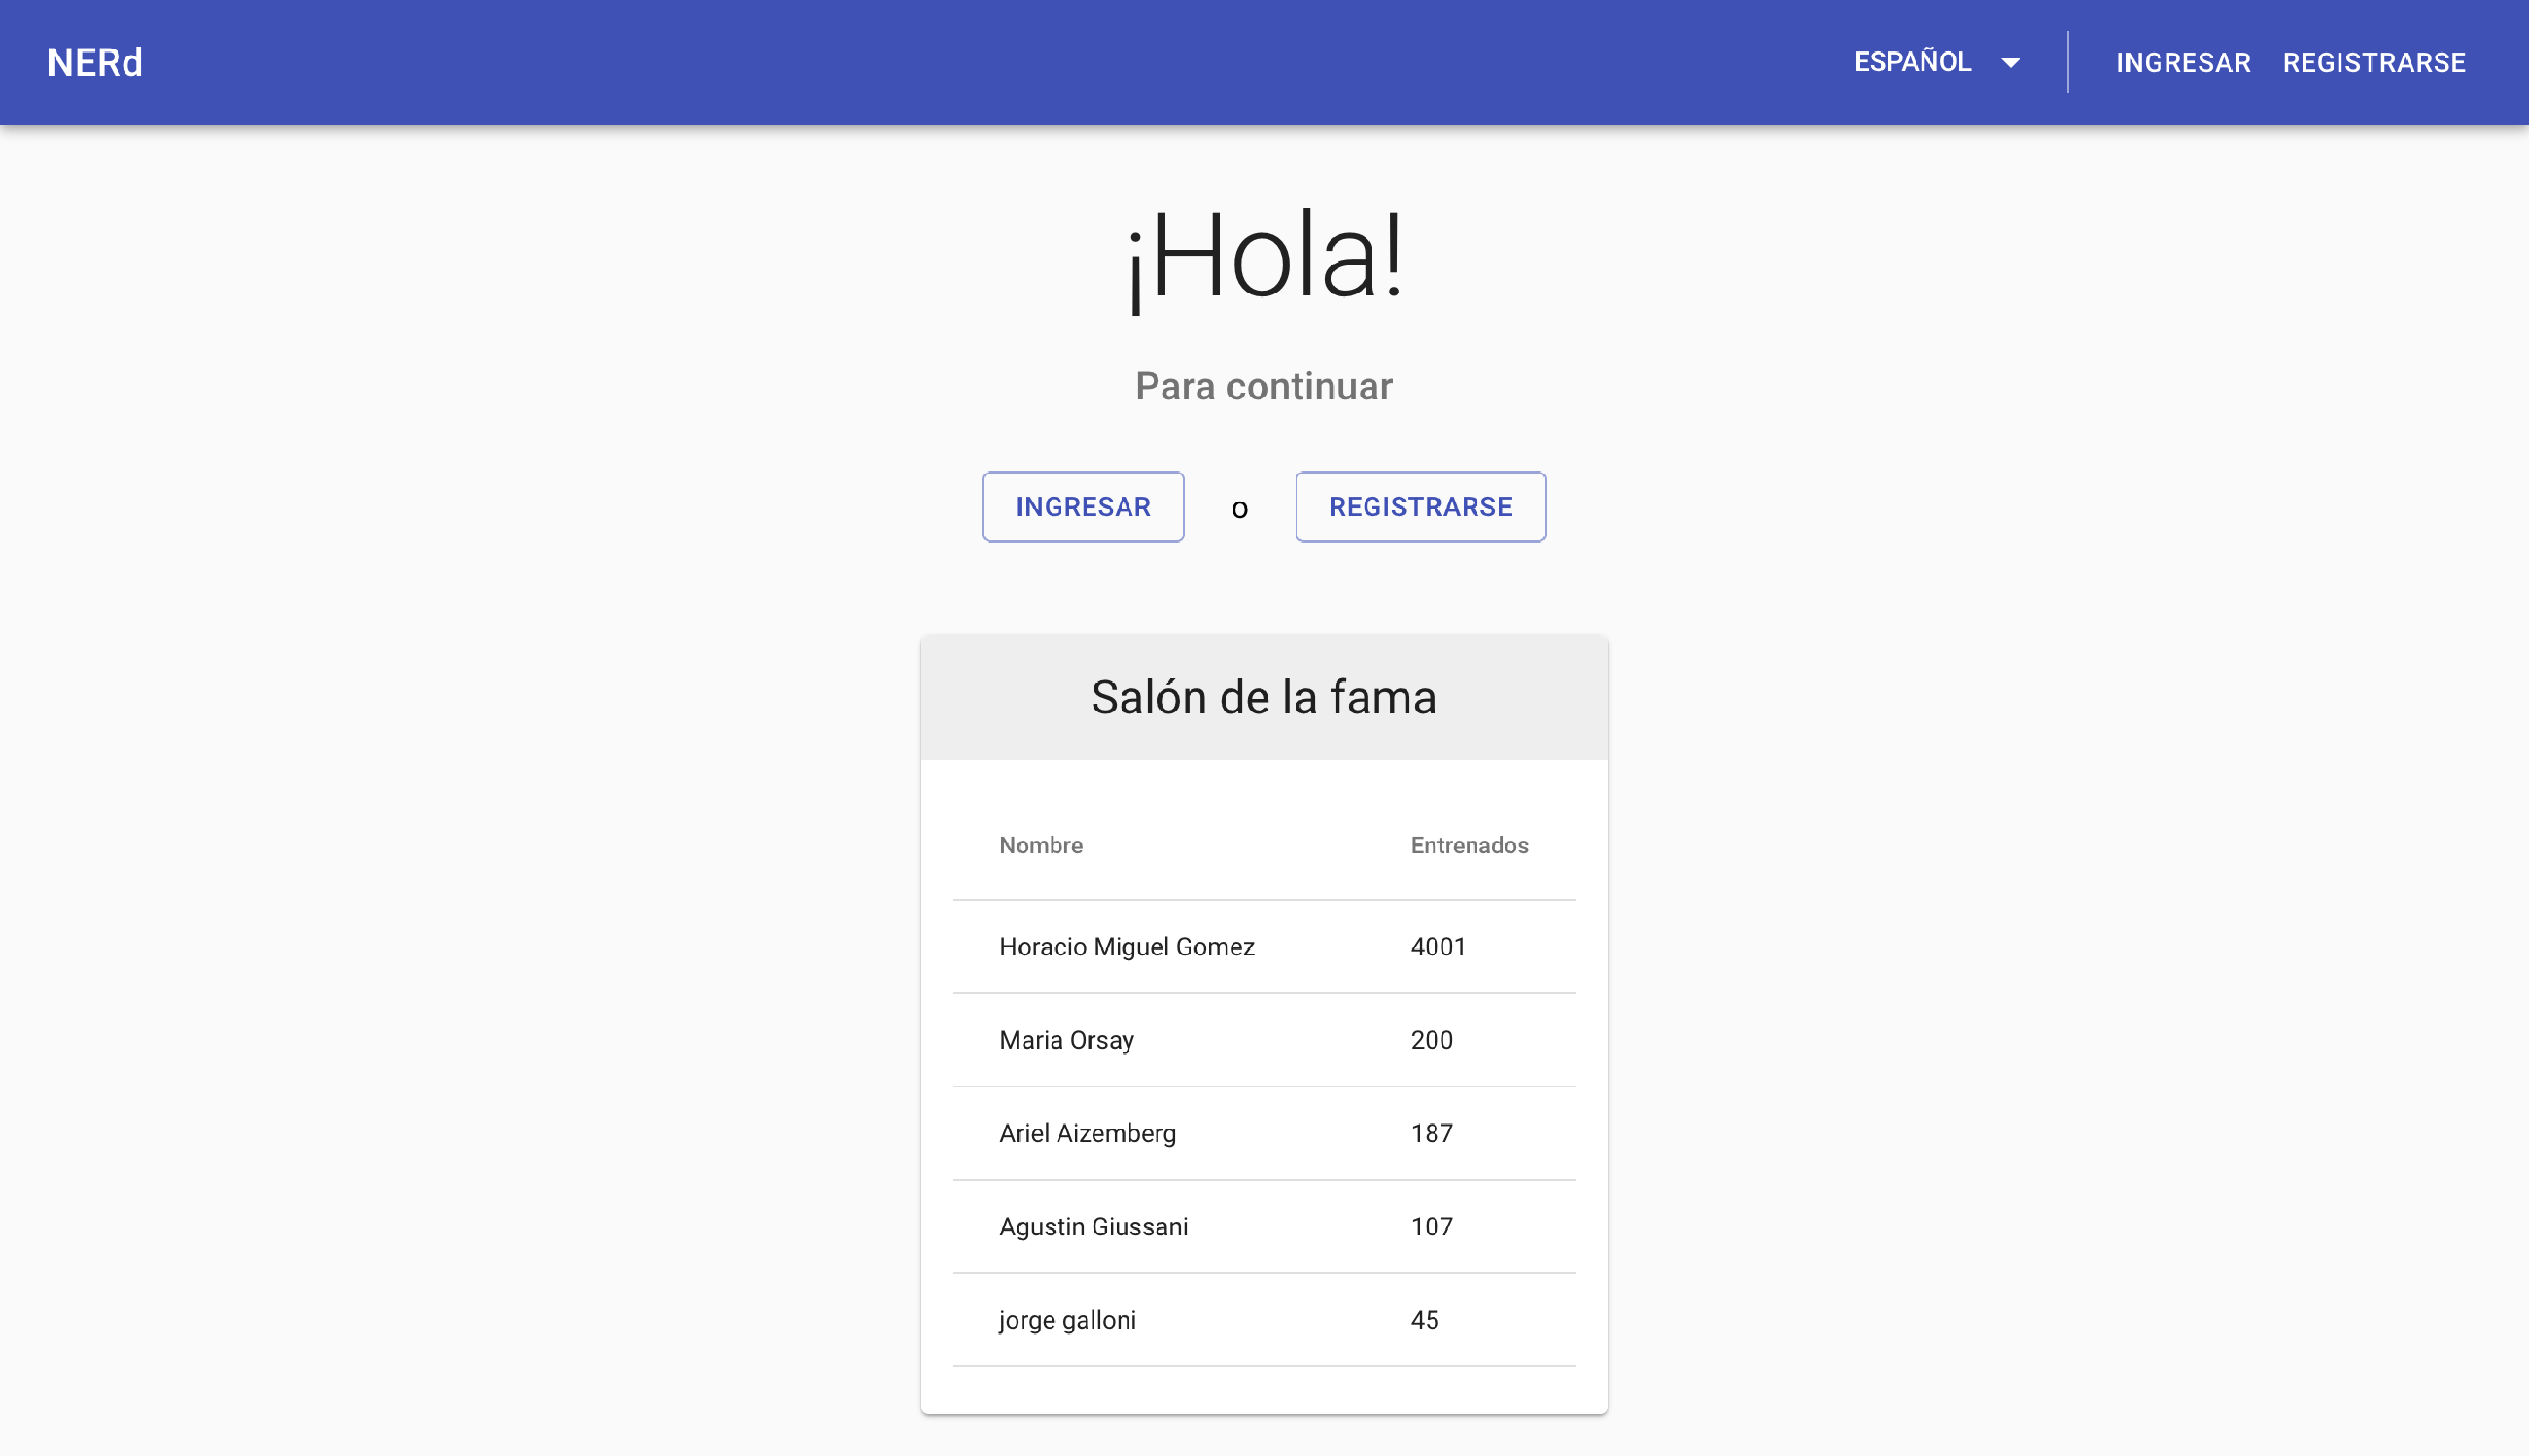
\includegraphics{assets/logic/home-anonymous.pdf} 

}

\caption{Pantalla de inicio sin sesión.}\label{fig:logic-home-anonymous}
\end{figure}

\hypertarget{entrenamiento}{%
\paragraph{Entrenamiento}\label{entrenamiento}}

La pantalla de entrenamiento es el núcleo de la \emph{web} donde se entrena el modelo.

El usuario es presentado con un texto perteneciente al \emph{corpus} del servicio con las entidades inferidas por el modelo actual. Con un editor especial, le permitimos al usuario poder corregir las entidades inferidas y enviarle la corrección al servicio. Esa corrección será utilizada posteriormente a la hora de mejorar el modelo actual (Figura \ref{fig:logic-train}).

\begin{figure}[H]

{\centering 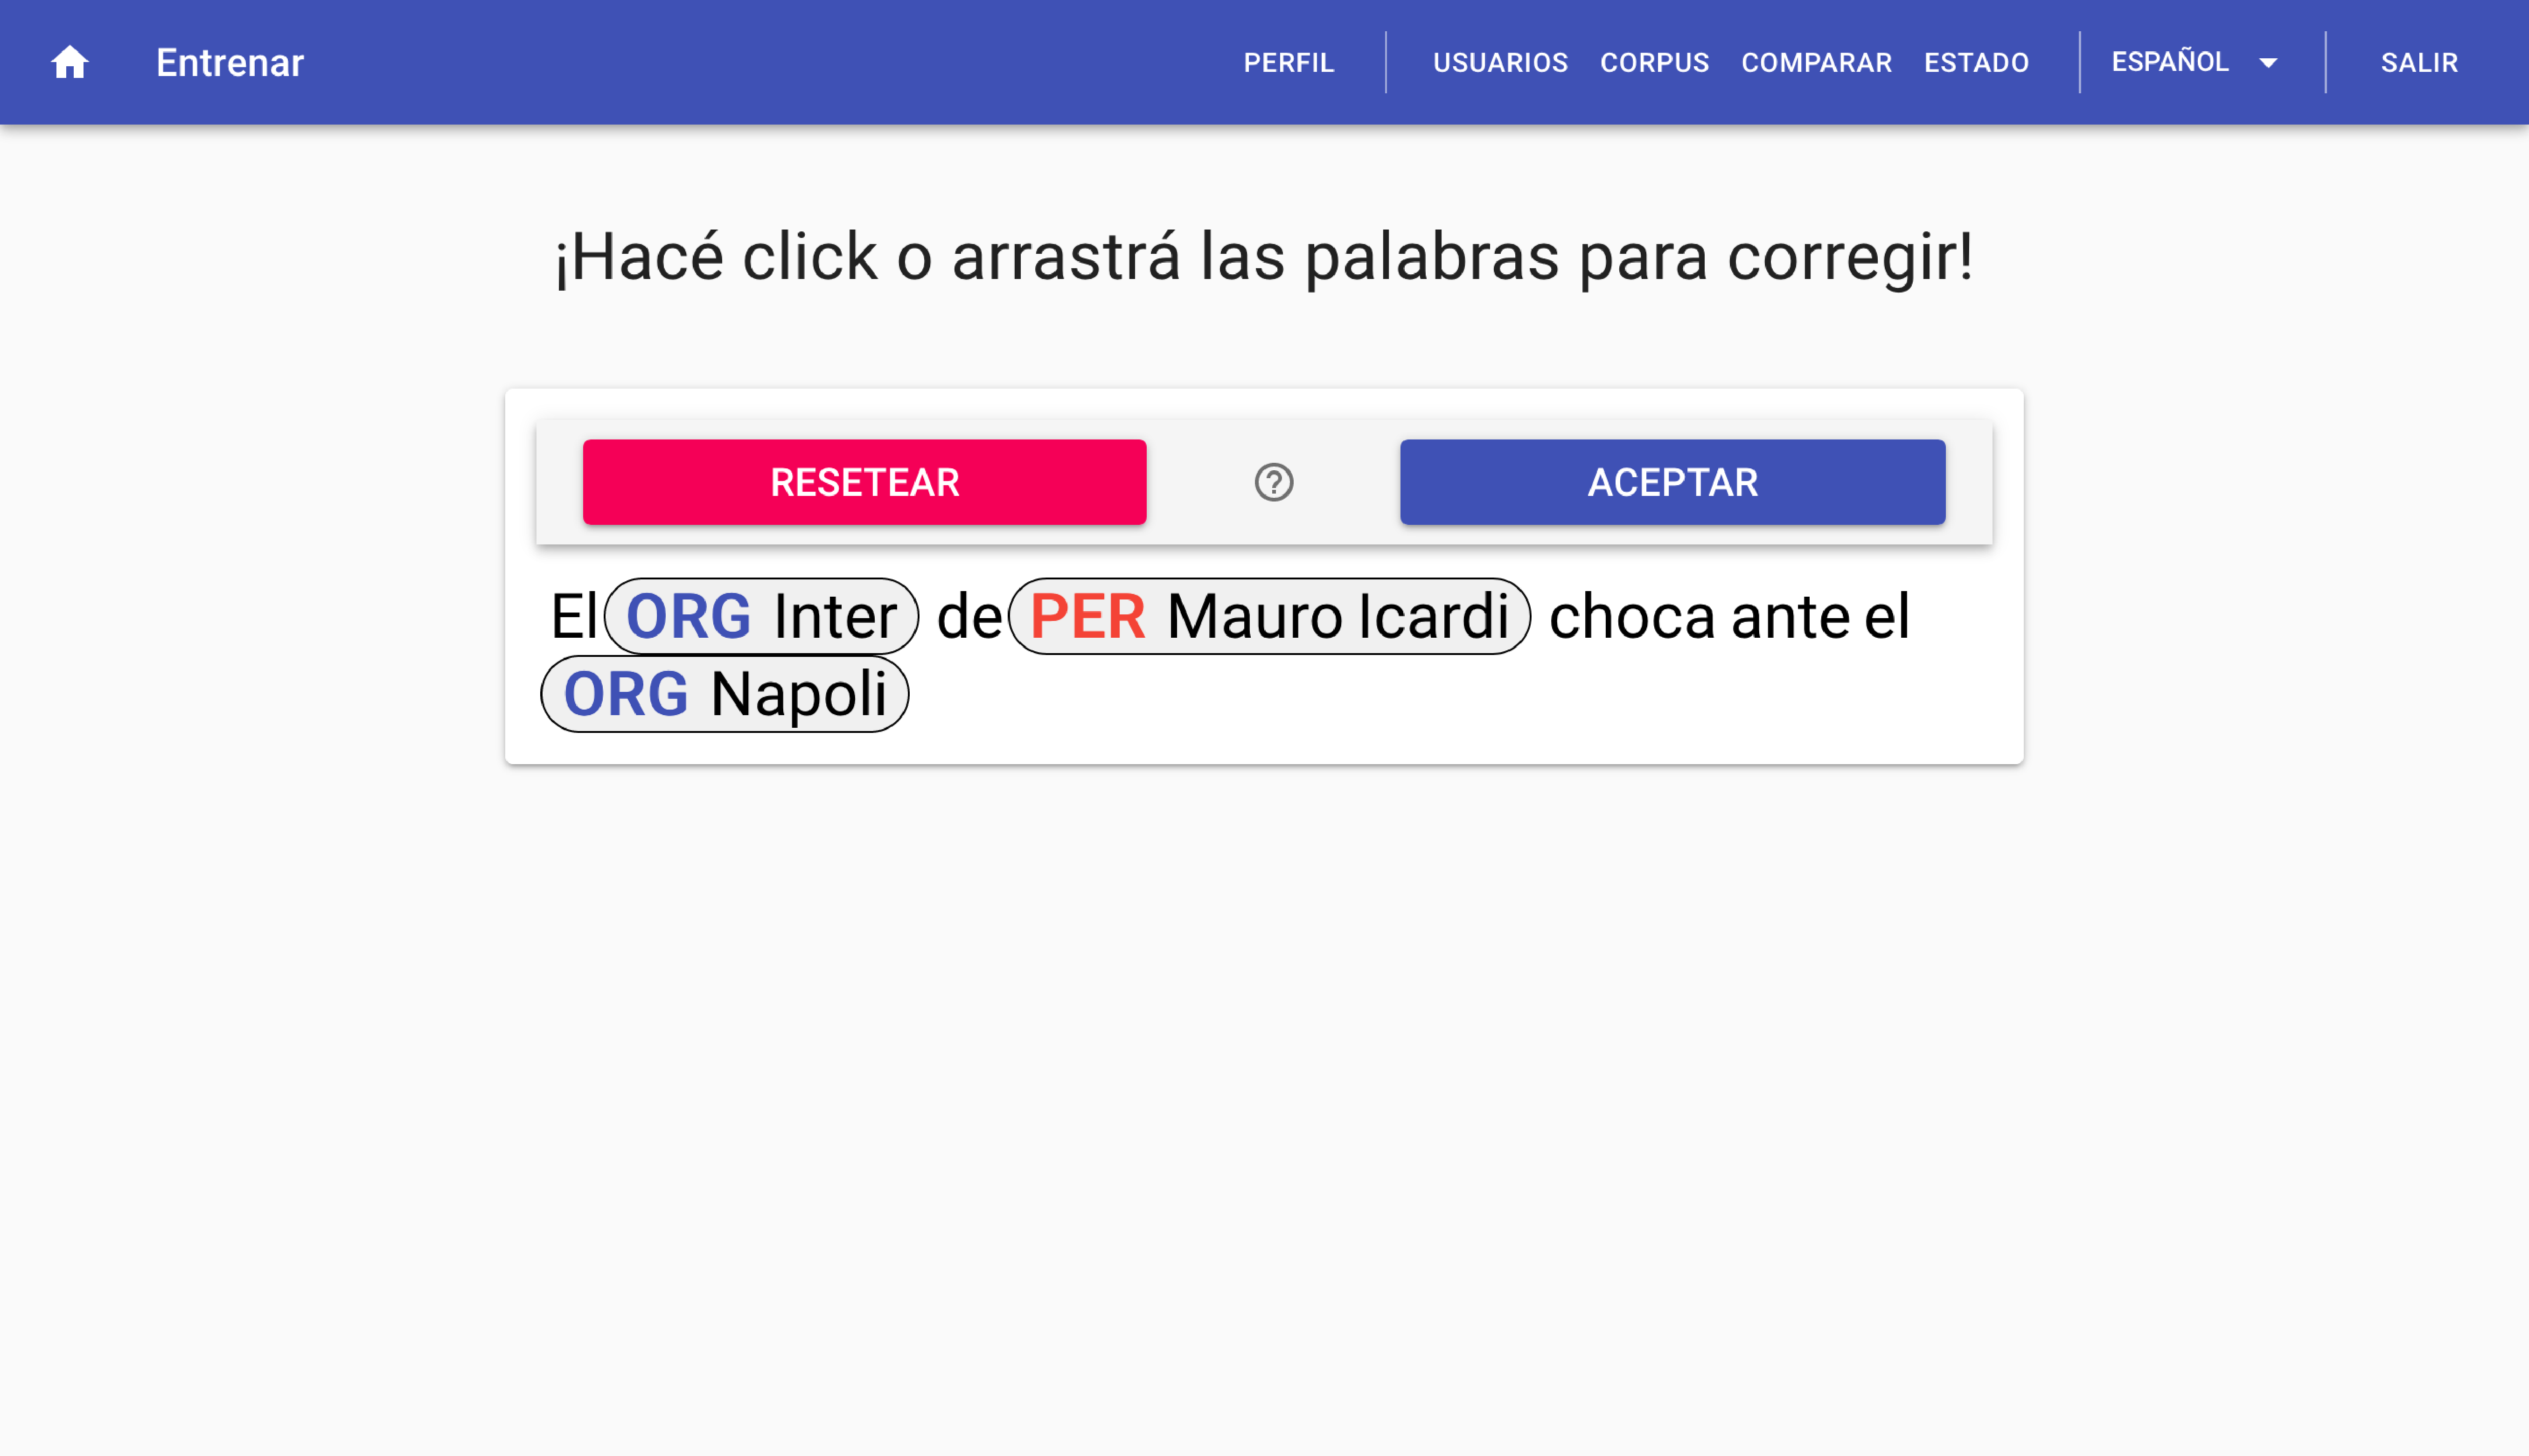
\includegraphics{assets/logic/train.pdf} 

}

\caption{Pantalla de entrenamiento.}\label{fig:logic-train}
\end{figure}

\hypertarget{usabilidad}{%
\subparagraph{Usabilidad}\label{usabilidad}}

Tuvimos un foco fuerte en la usabilidad del componente ya que los entrenadores del servicio van a pasar prácticamente todo su tiempo en ésta pantalla, por lo que se tuvieron las siguientes consideraciones en la implementación.

Llamado a acción y ayuda

Dado que lo primero que ve el usuario es un texto con etiquetas de entidad, agregamos un título que invita al usuario a realizar acciones sobre el texto. De esta manera, le mostramos las dos acciones principales realizables desde el componente de entrenamiento: Click en alguna palabra o entidad y arrastrar un conjunto de palabras para crear una entidad nueva.
Como refuerzo de este llamado a acción, agregamos un botón que al ser clickeado muestra un mensaje de ayuda con instrucciones más detalladas sobre el objetivo del entrenador y las acciones que deben de realizarse sobre el mismo (Figura \ref{fig:logic-train-help}).

\begin{figure}[H]

{\centering 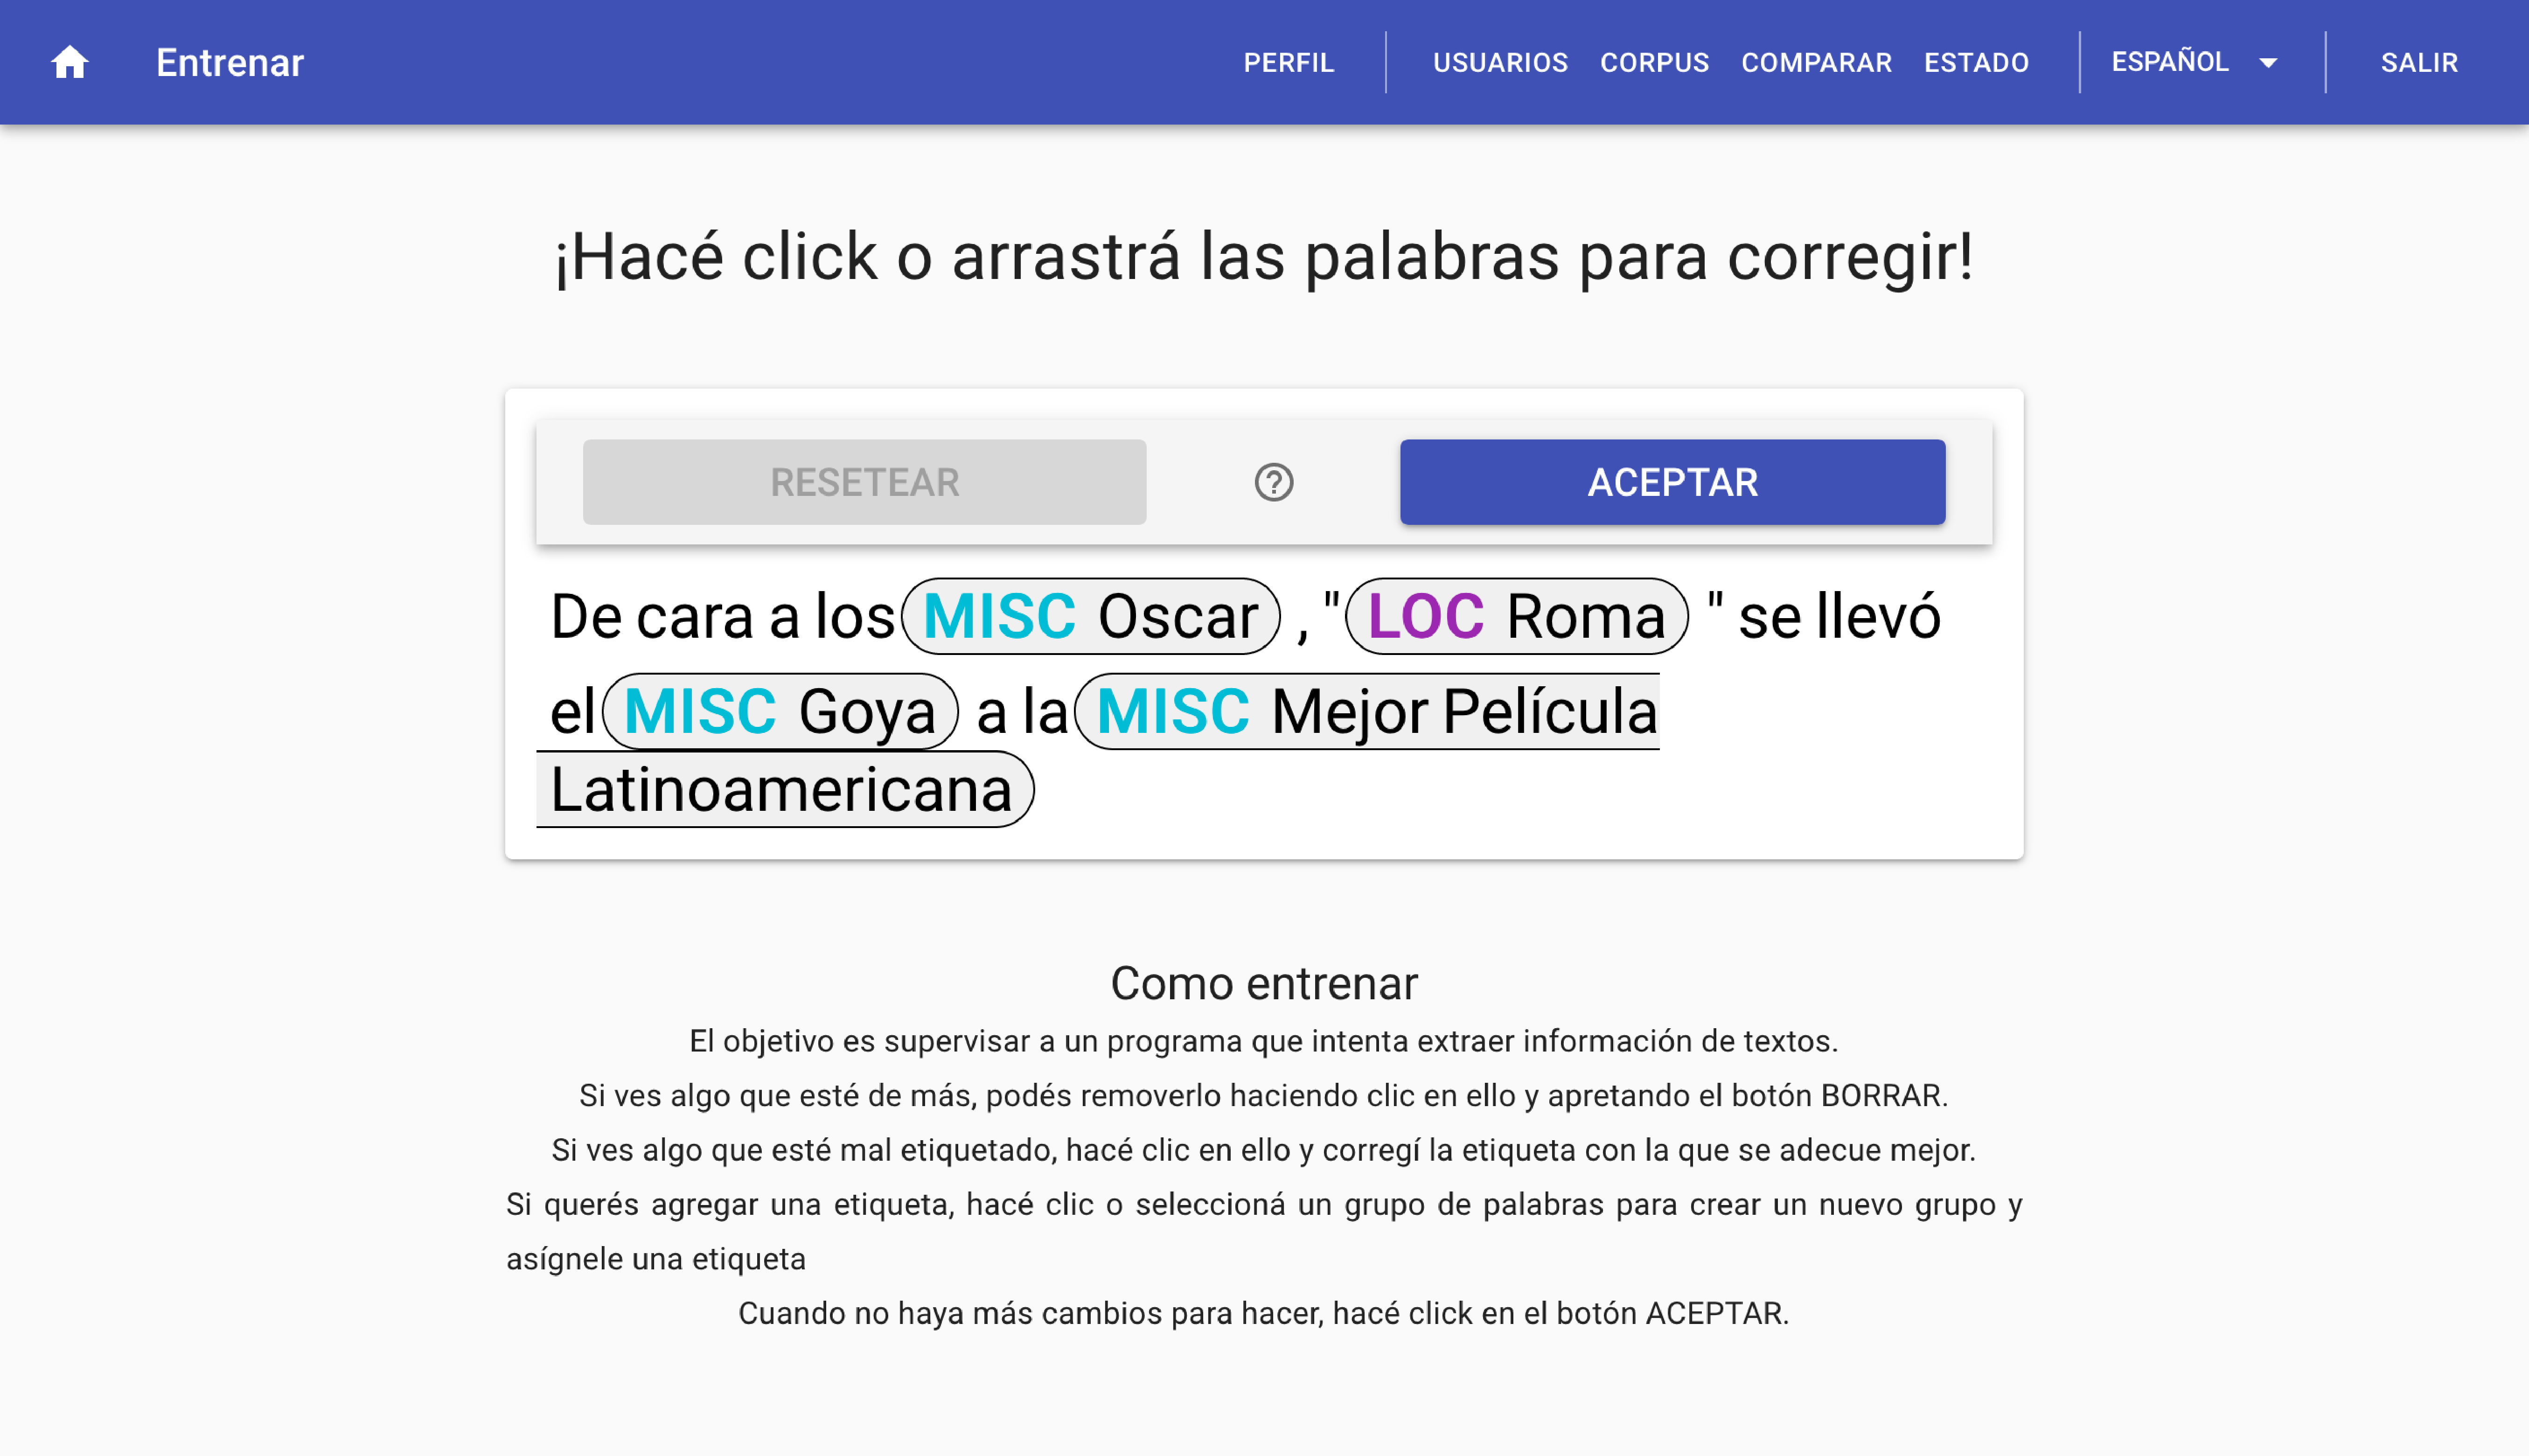
\includegraphics{assets/logic/train-help.pdf} 

}

\caption{Ayuda del entrenador.}\label{fig:logic-train-help}
\end{figure}

Etiquetado de entidades

Para etiquetar entidades decidimos ofrecer dos maneras: La más sencilla es hacer click en cada palabra. La segunda, para cuando una entidad esta definida por múltiples palabras, es arrastrar el cursor entre ellas.
Dependiendo de la ubicación en la selección dentro del texto:

\begin{itemize}
\tightlist
\item
  Si no existen entidades en el texto actual, se le asigna por defecto el tipo \emph{MISC} y se muestran el resto de los tipos para permitir cambiarlo de ser necesario.
\item
  Si existen entidades antes o después, se ofrece la opción de unir la palabra actual con la entidada más próxima para el lado elegido.
\end{itemize}

\begin{figure}[H]

{\centering 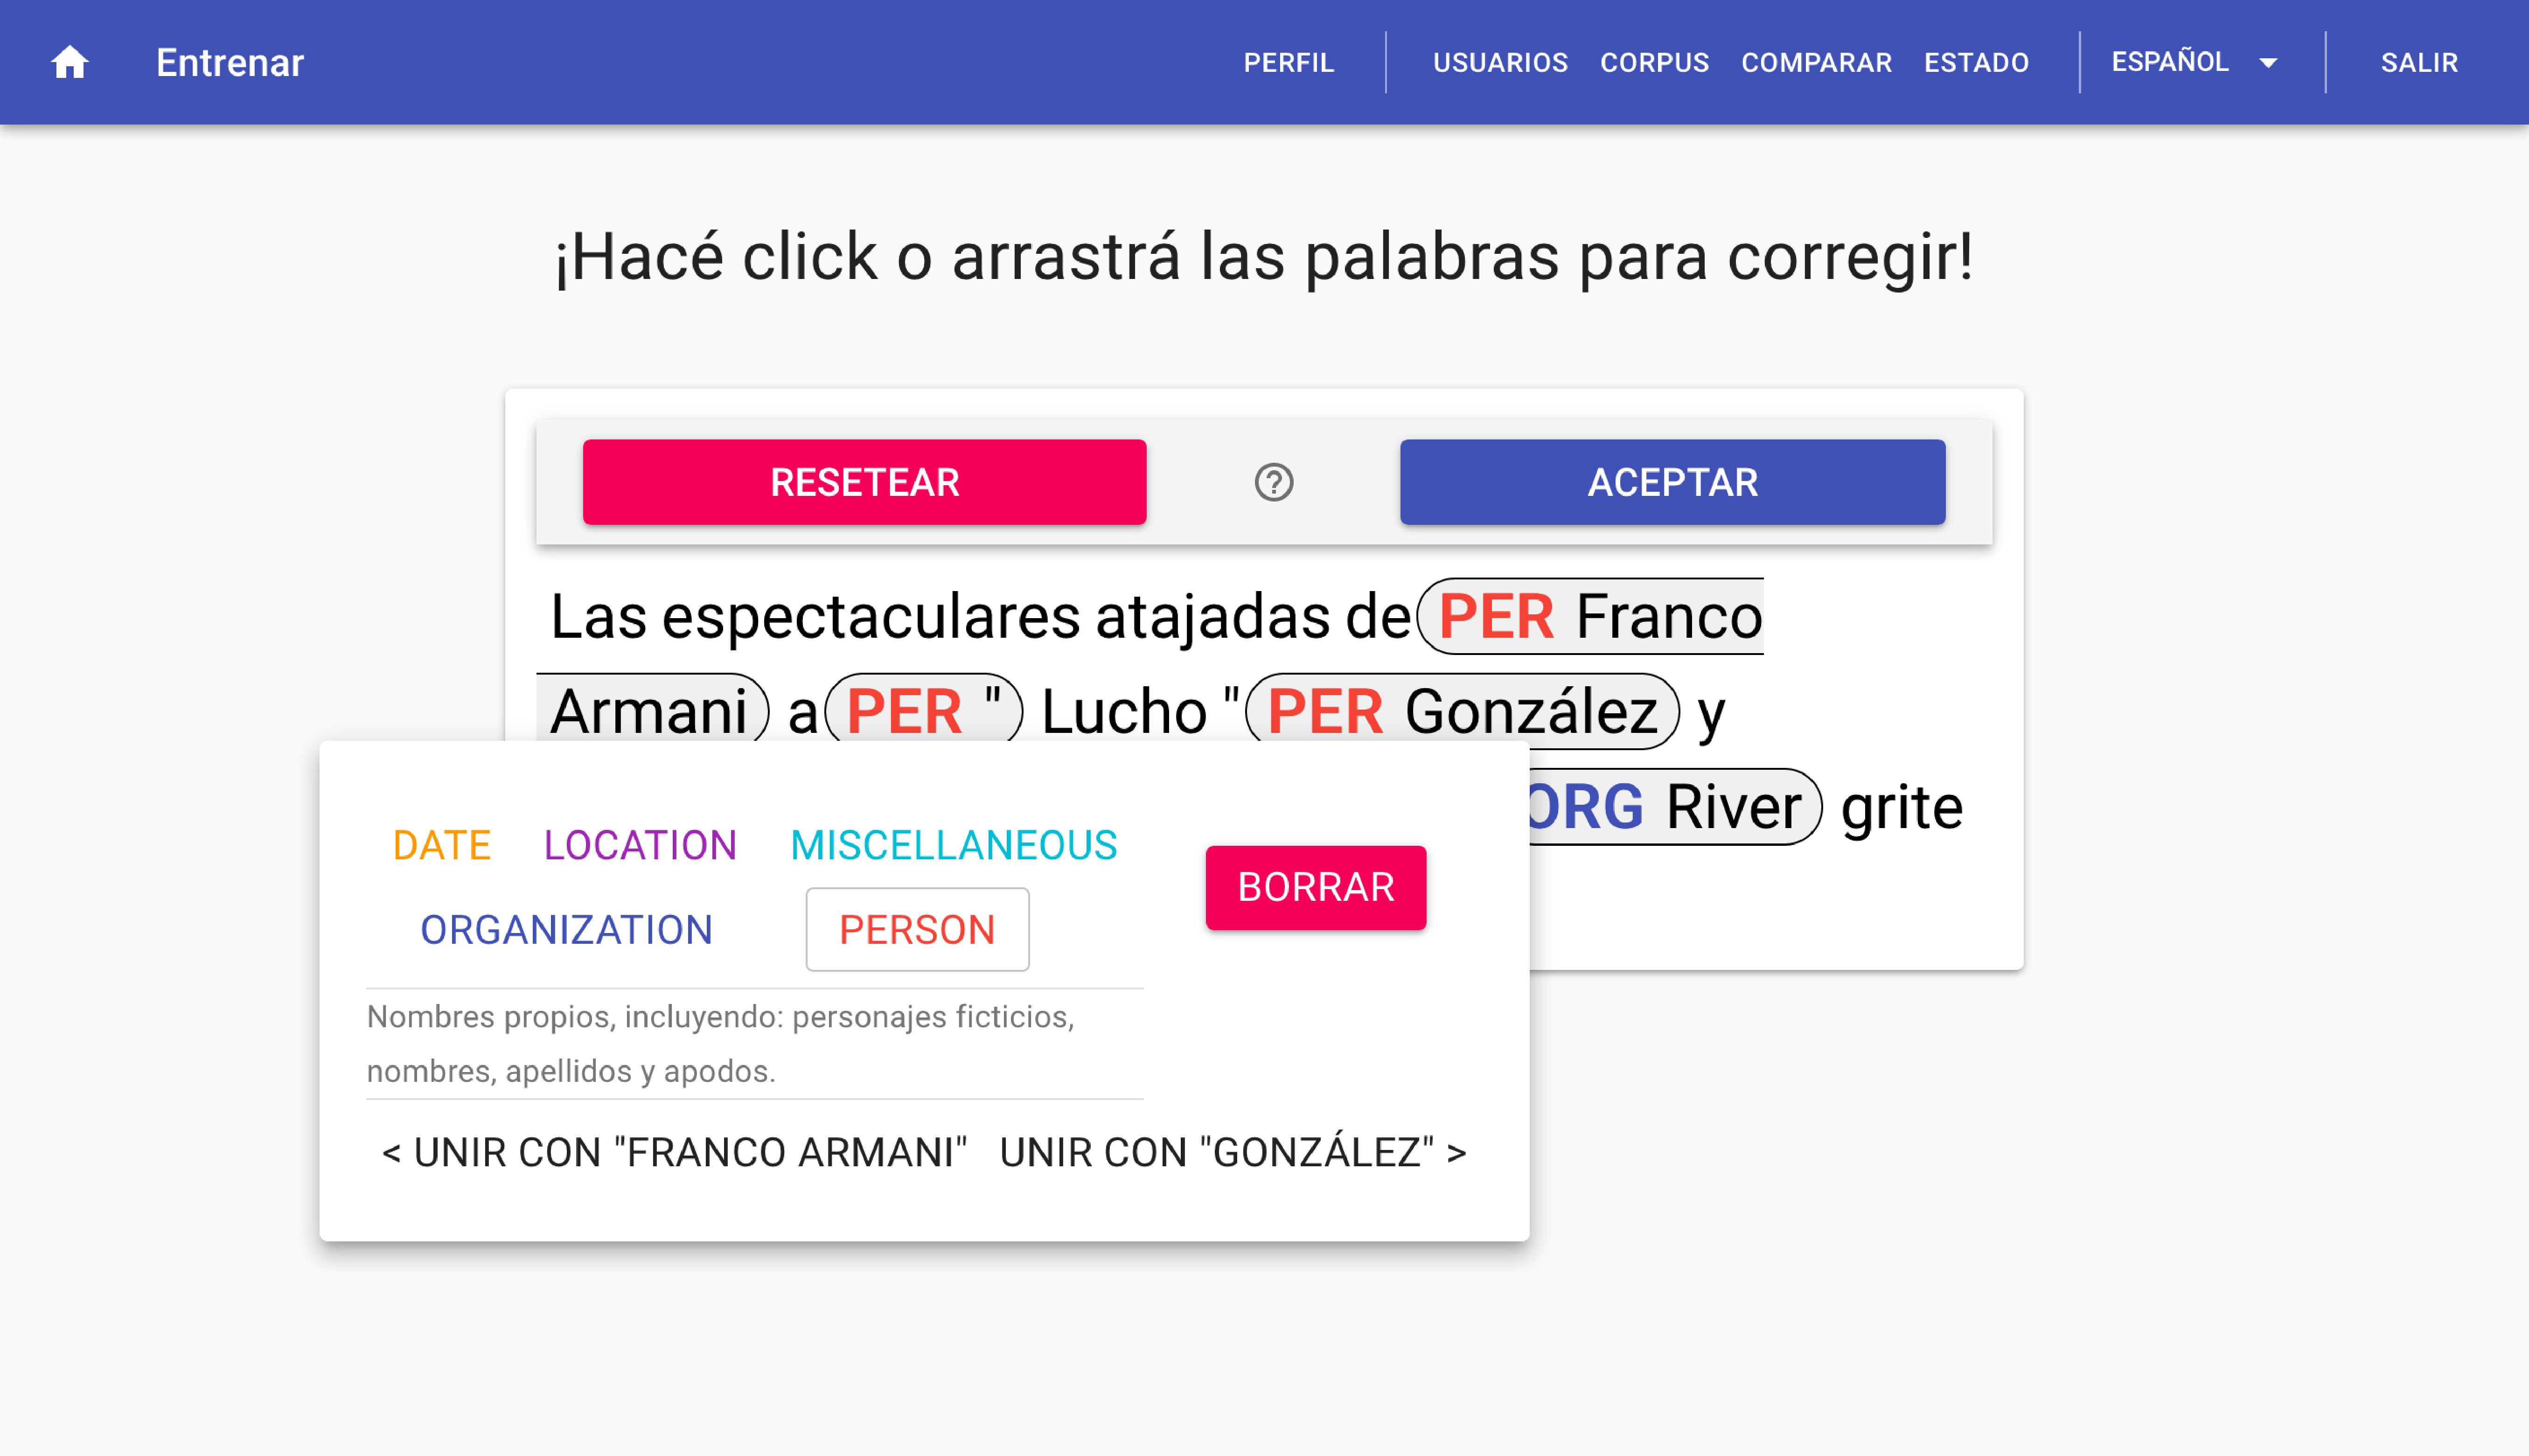
\includegraphics{assets/logic/train-popup.pdf} 

}

\caption{Edición de entidad.}\label{fig:logic-train-popup}
\end{figure}

Como podemos ver en la figura \ref{fig:logic-train-popup}, si el modelo infirió una entidad de manera incorrecta, ya sea por que se trata de una entidad inválida o agregó palabras de más a la etiqueta, permitimos que el usuario remueva la entidad y que después vuelva a etiquetar correctamente.

Optimización en tiempos de carga

Es esperado que un usuario entrene más de un texto, al momento de pedir un texto para mostrar, se pide el siguiente. Mediante este mecanismo de pre-carga, podemos eliminar el tiempo de espera entre texto y texto ofreciendo al usuario entrenador una experiencia completamente fluida.

\hypertarget{administraciuxf3n-de-usuarios}{%
\paragraph{Administración de usuarios}\label{administraciuxf3n-de-usuarios}}

La pantalla de \emph{Administración de usuarios} permite a los usuarios con el rol de administrador poder modificar los roles de todos los usuarios del sistema, borrarlos o acceder a los detalles del usuario, tal como la lista de textos entrenados (Figura \ref{fig:logic-user-list}).

\begin{figure}[H]

{\centering 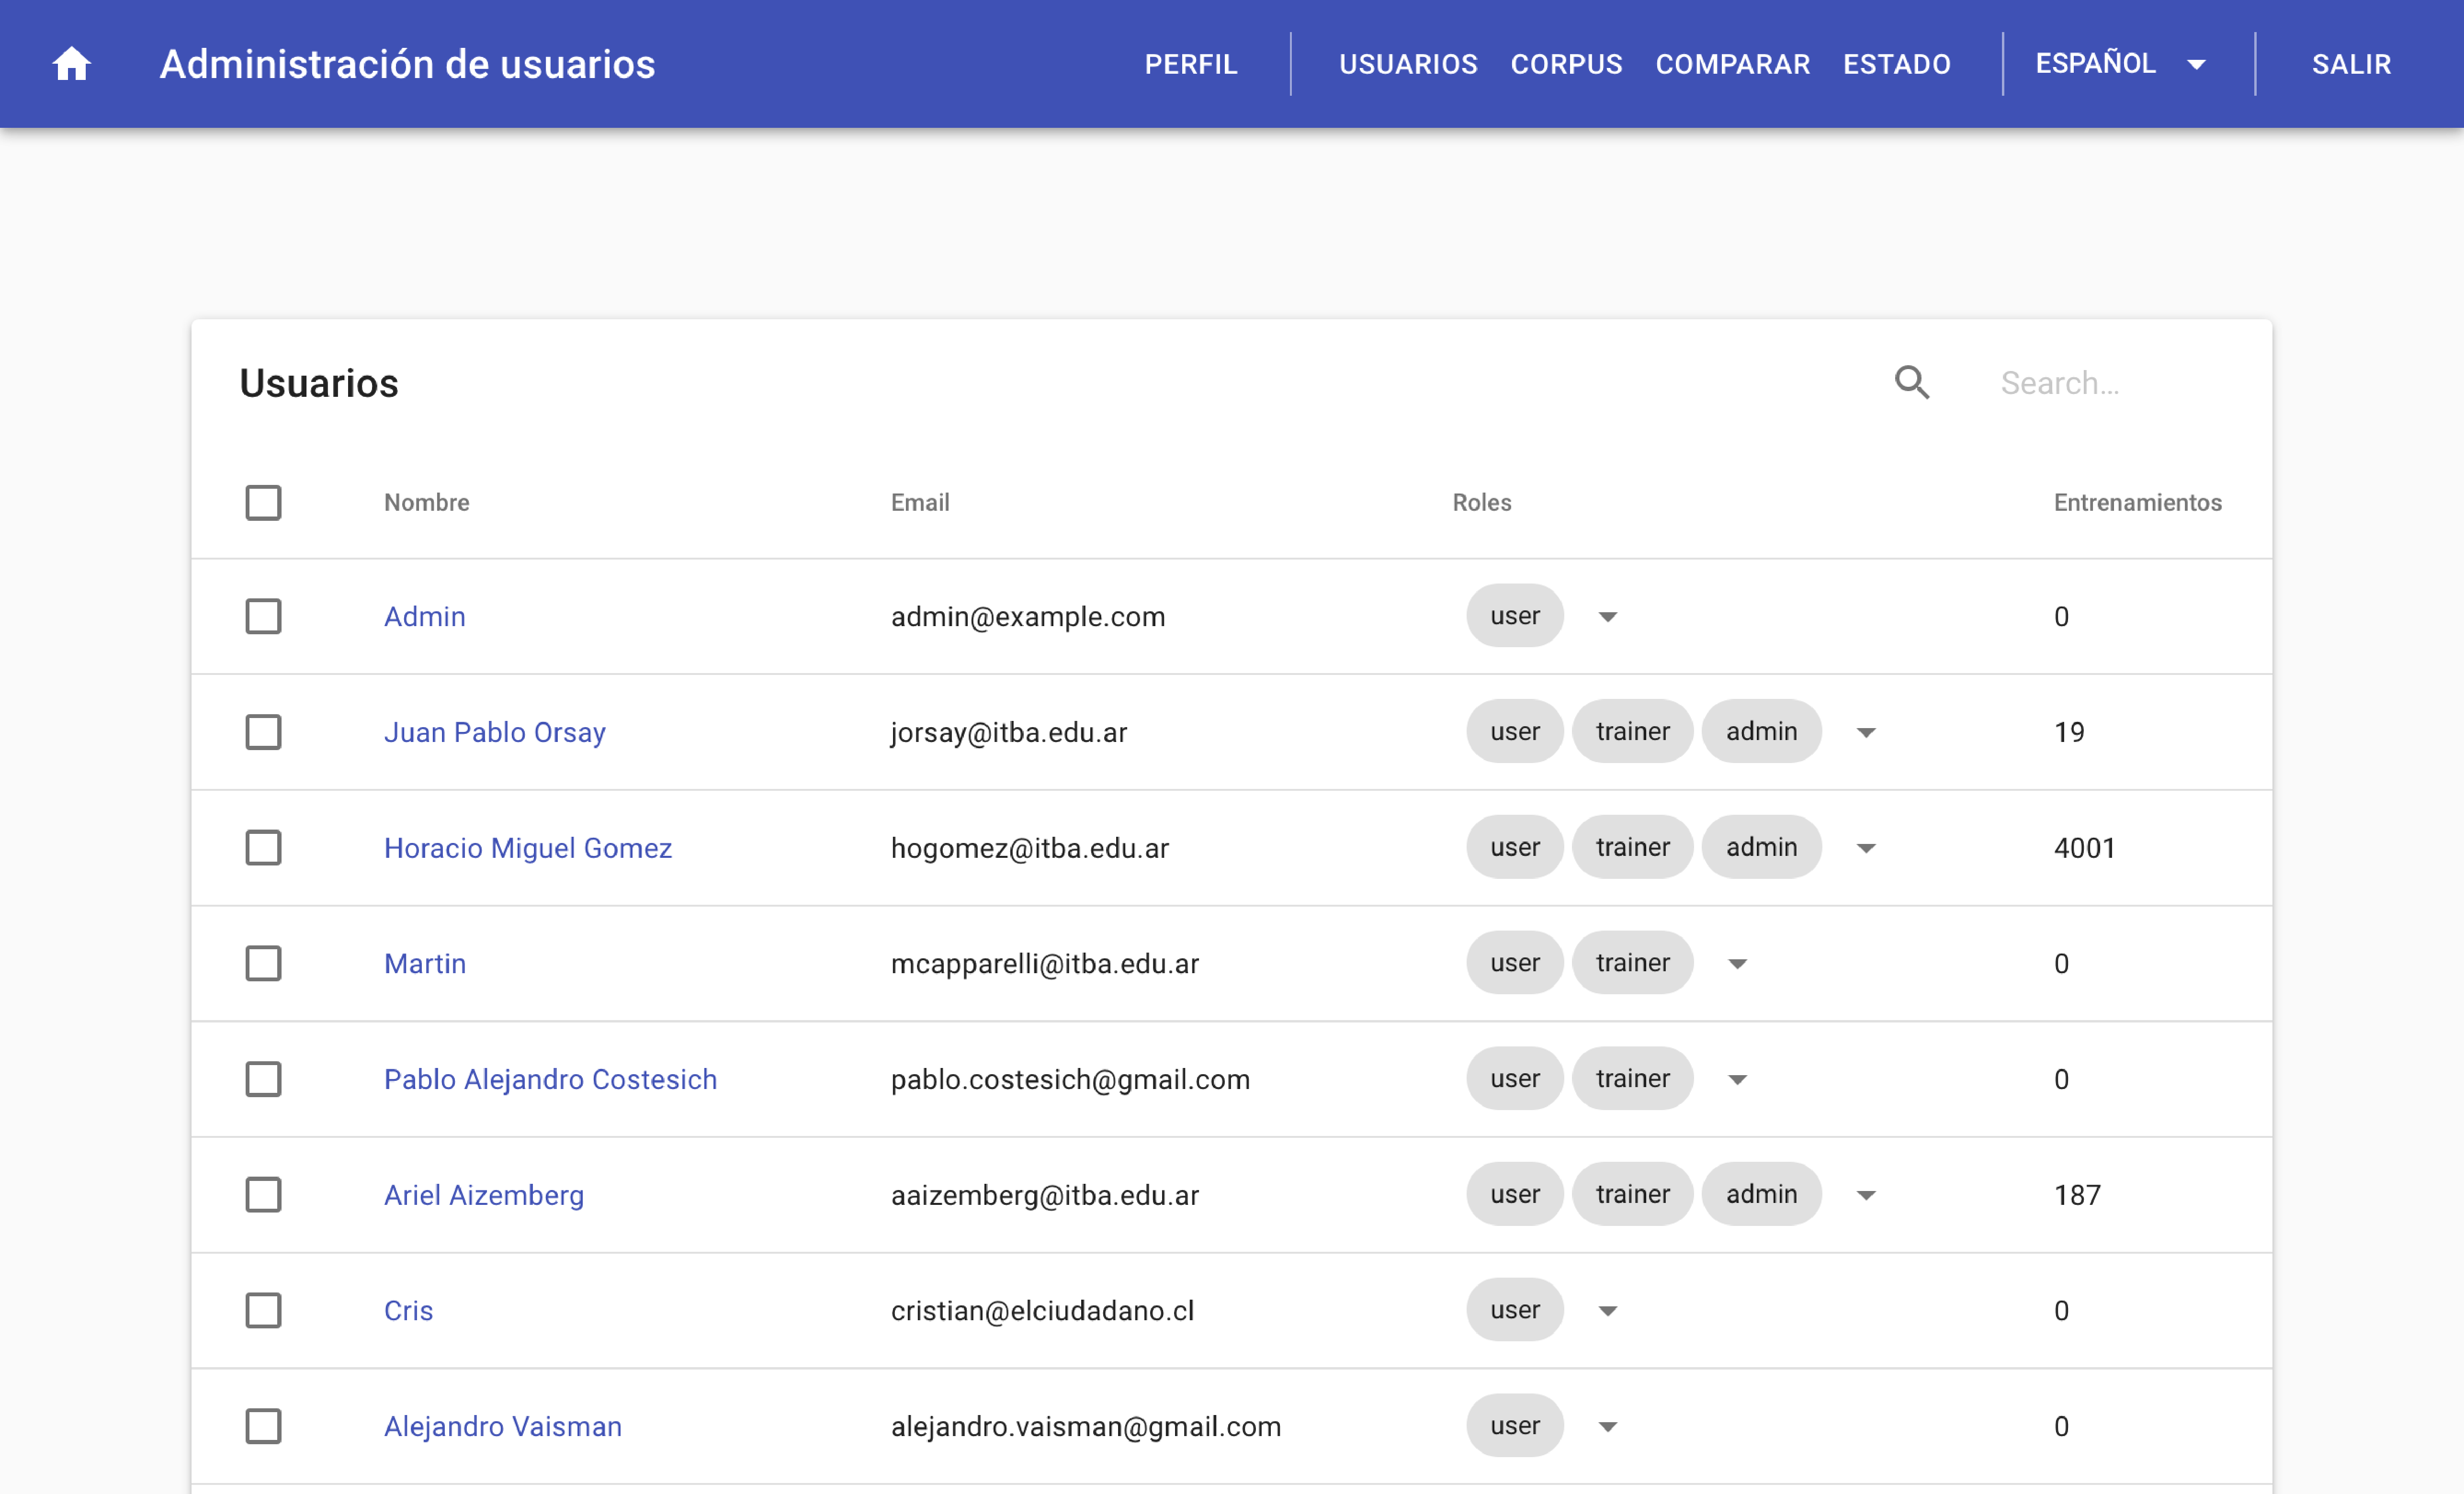
\includegraphics{assets/logic/user-list.pdf} 

}

\caption{Administración de usuarios.}\label{fig:logic-user-list}
\end{figure}

\hypertarget{perfil-del-usuario}{%
\paragraph{Perfil del usuario}\label{perfil-del-usuario}}

Al hacer click Perfil, el usuario con sesión activa puede ver sus entrenamientos y cambiar su contraseña (Figura \ref{fig:logic-user-profile}).

\begin{figure}[H]

{\centering 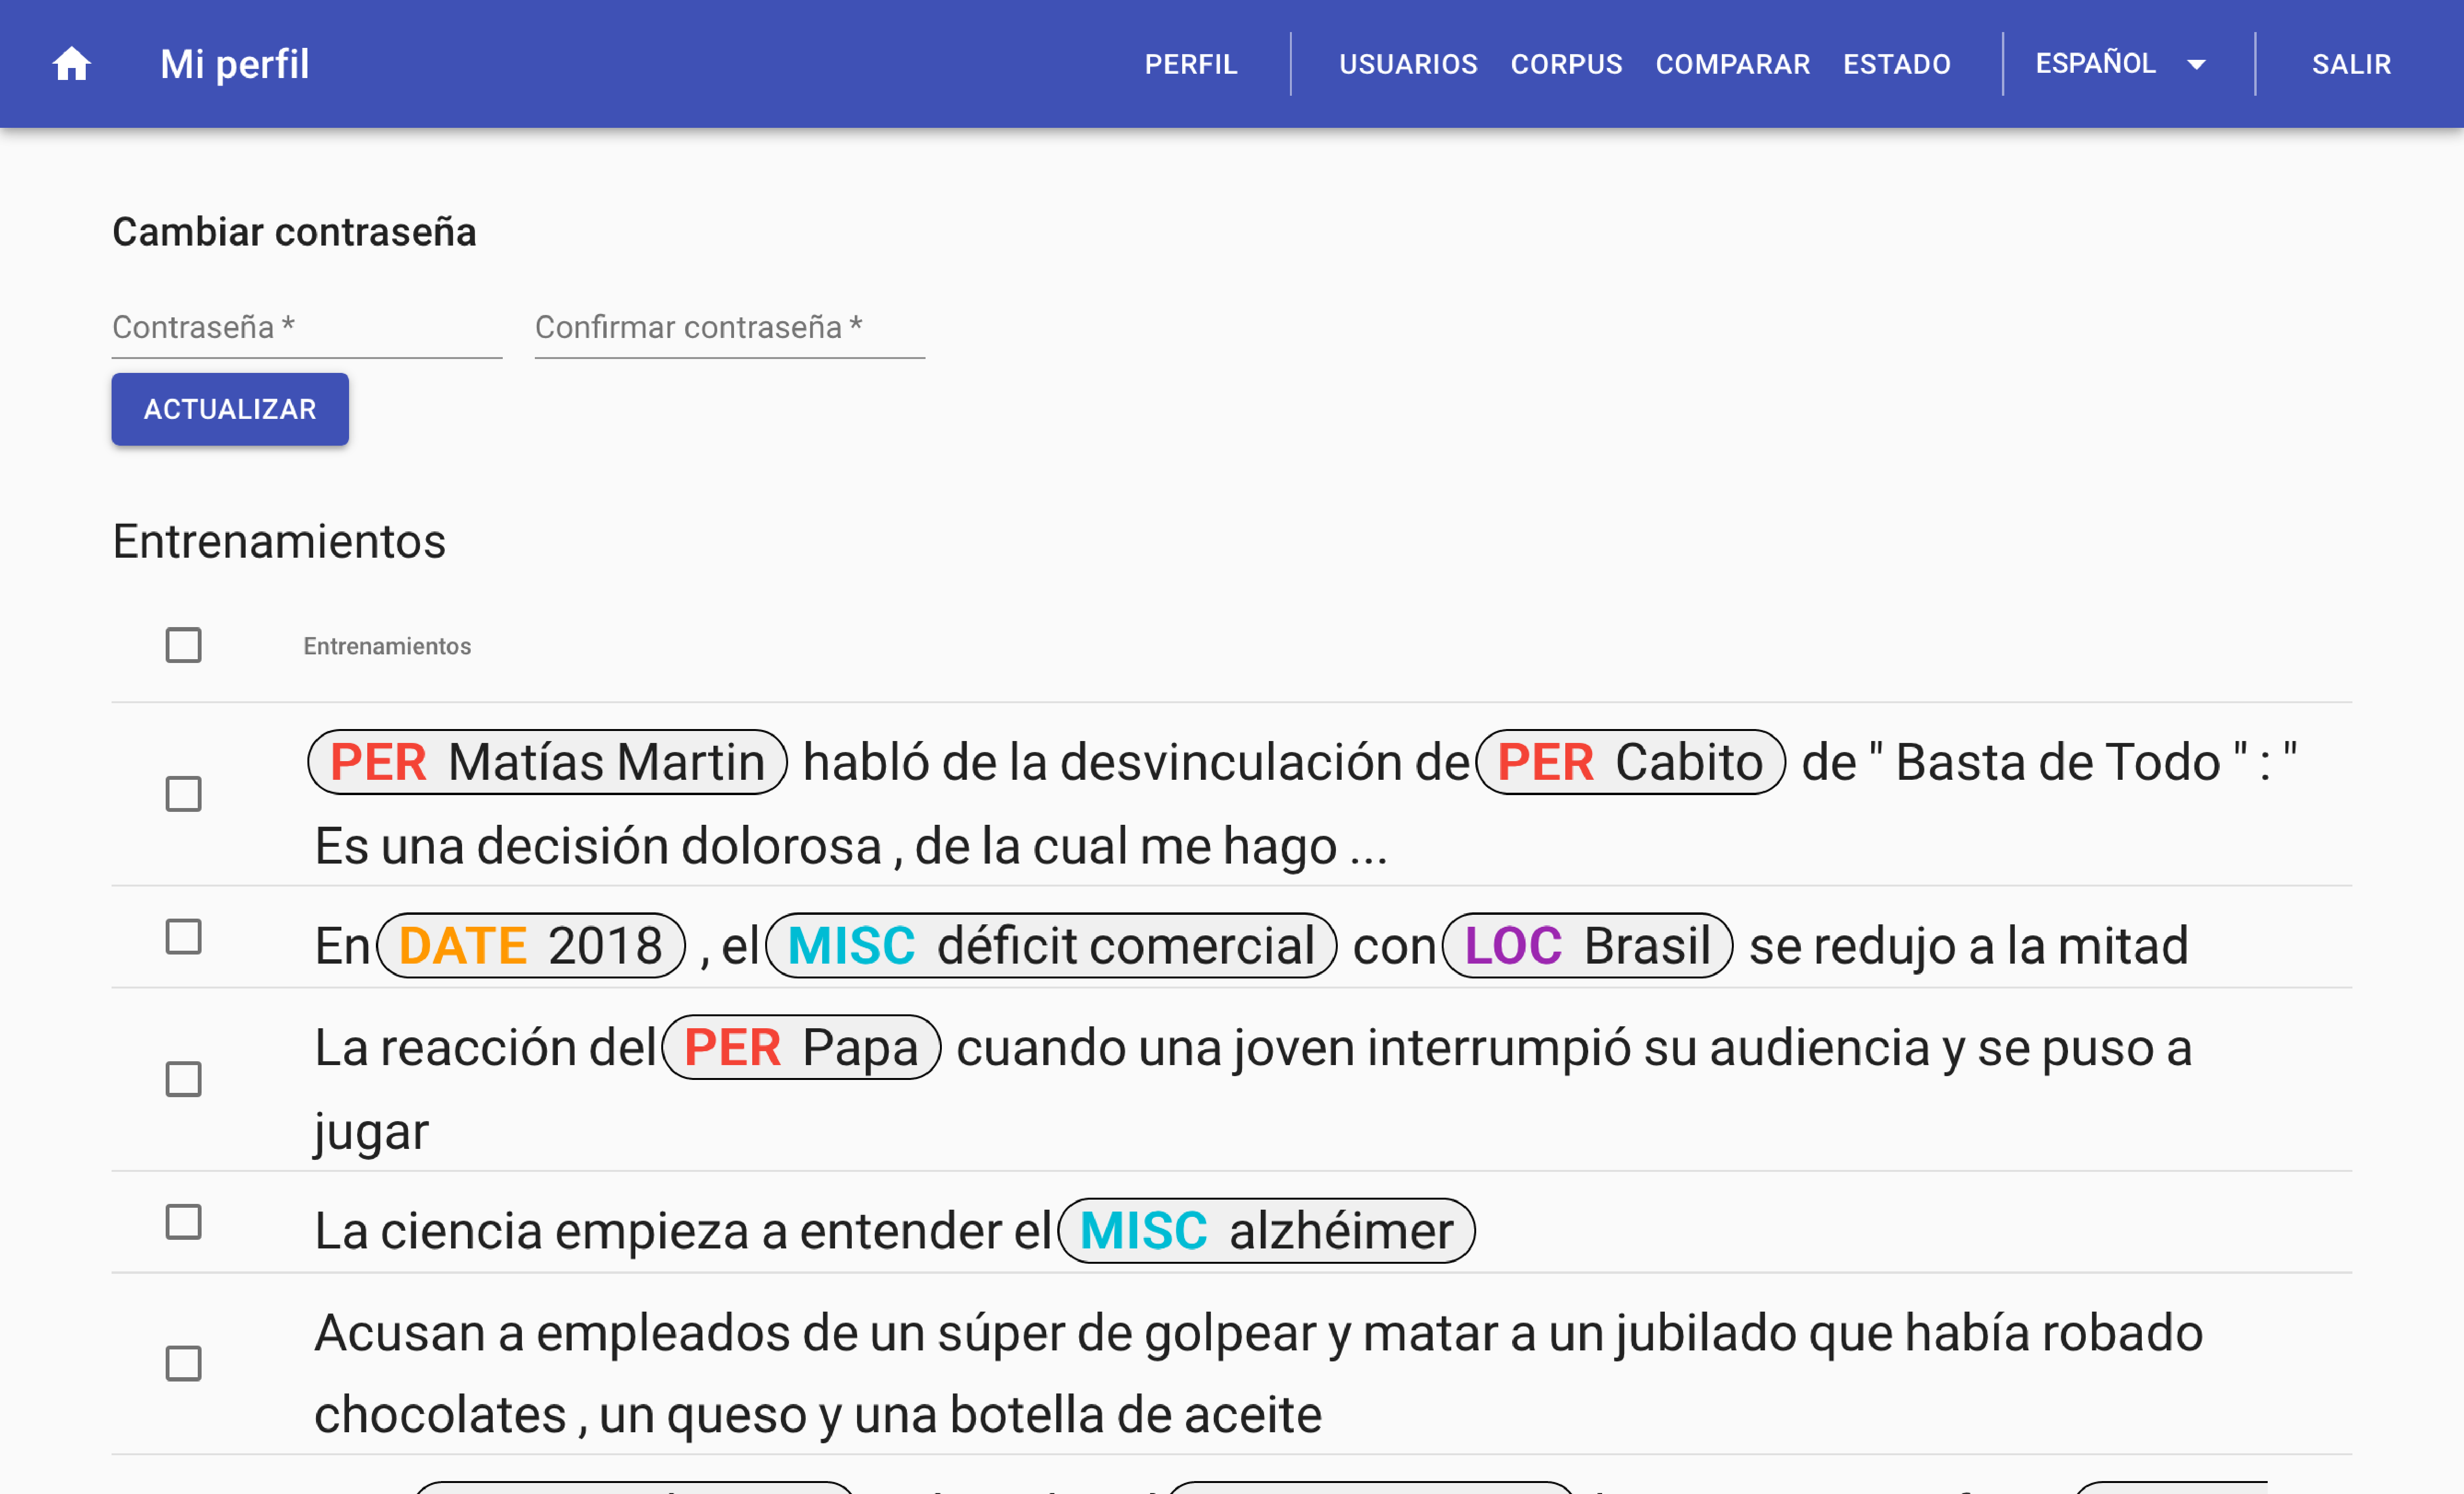
\includegraphics{assets/logic/user-profile.pdf} 

}

\caption{Perfil de usuario.}\label{fig:logic-user-profile}
\end{figure}

Los usuarios con rol administrador pueden realizar las acciones mencionadas previamente pero sobre cualquier usuario haciendo click en el nombre del en la figura \ref{fig:logic-user-list}.

\hypertarget{corpus}{%
\paragraph{\texorpdfstring{\emph{Corpus}}{Corpus}}\label{corpus}}

La pantalla de \emph{corpus} permite a un usuario con el rol de administrador realizar tareas relacionadas con el conjunto de textos ingresados en el sistema (Figura \ref{fig:logic-corpus-management}).

\begin{figure}[H]

{\centering 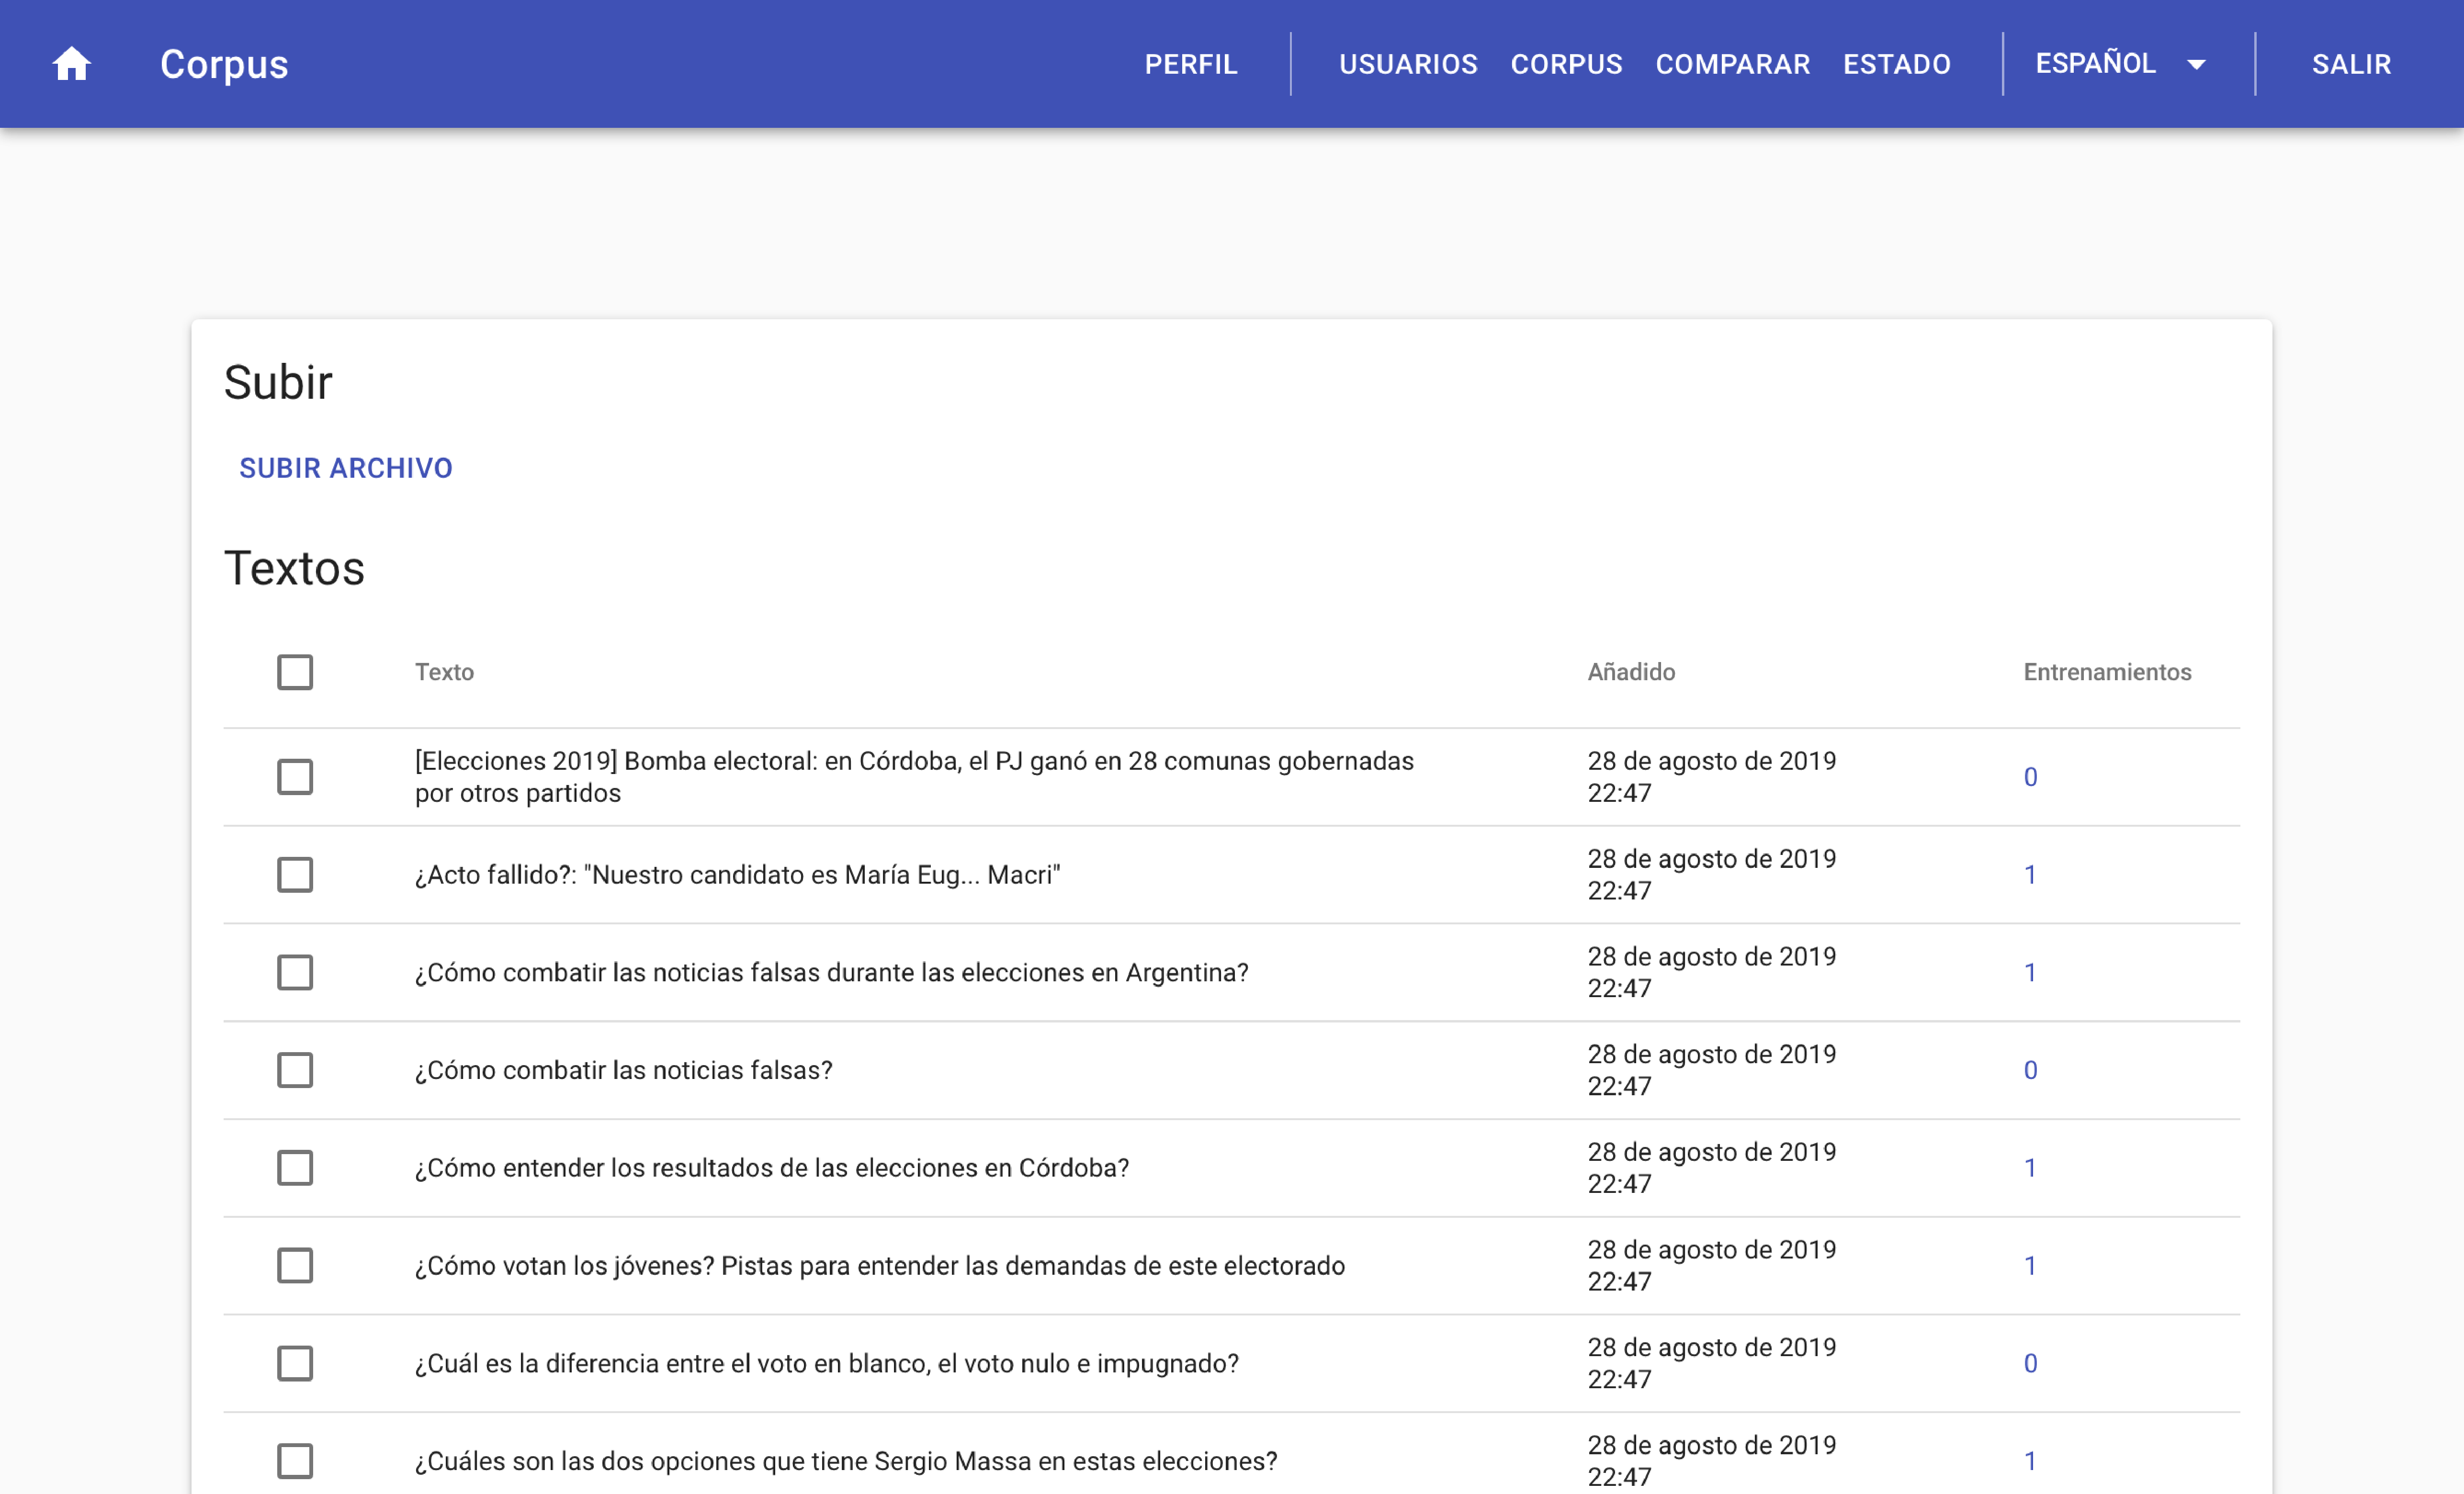
\includegraphics{assets/logic/corpus-management.pdf} 

}

\caption{Administración de corpus.}\label{fig:logic-corpus-management}
\end{figure}

Desde aquí es posible agregar textos al \emph{corpus} utilizando la funcionalidad de subida de archivos. Los archivos deben ser archivos con extensión \emph{.txt} y cada línea del archivo será agregada al \emph{corpus} como un texto individual.

También es posible desde aquí ver todos los textos que forman parte del \emph{corpus} así como también poder ver los entrenamientos para cada uno de los textos. Finalmente, es posible quitar textos del \emph{corpus} así como también eliminar correcciones a las inferencias de entidades cargados por usuarios.

\hypertarget{estado}{%
\paragraph{Estado}\label{estado}}

La pantalla de \emph{Estado} permite a un usuario con el rol de administrador visualizar el estado de entrenamiento del \emph{corpus} así como también realizar diversas acciones sobre los \emph{workers} (Figura \ref{fig:logic-status}).

\begin{figure}[H]

{\centering 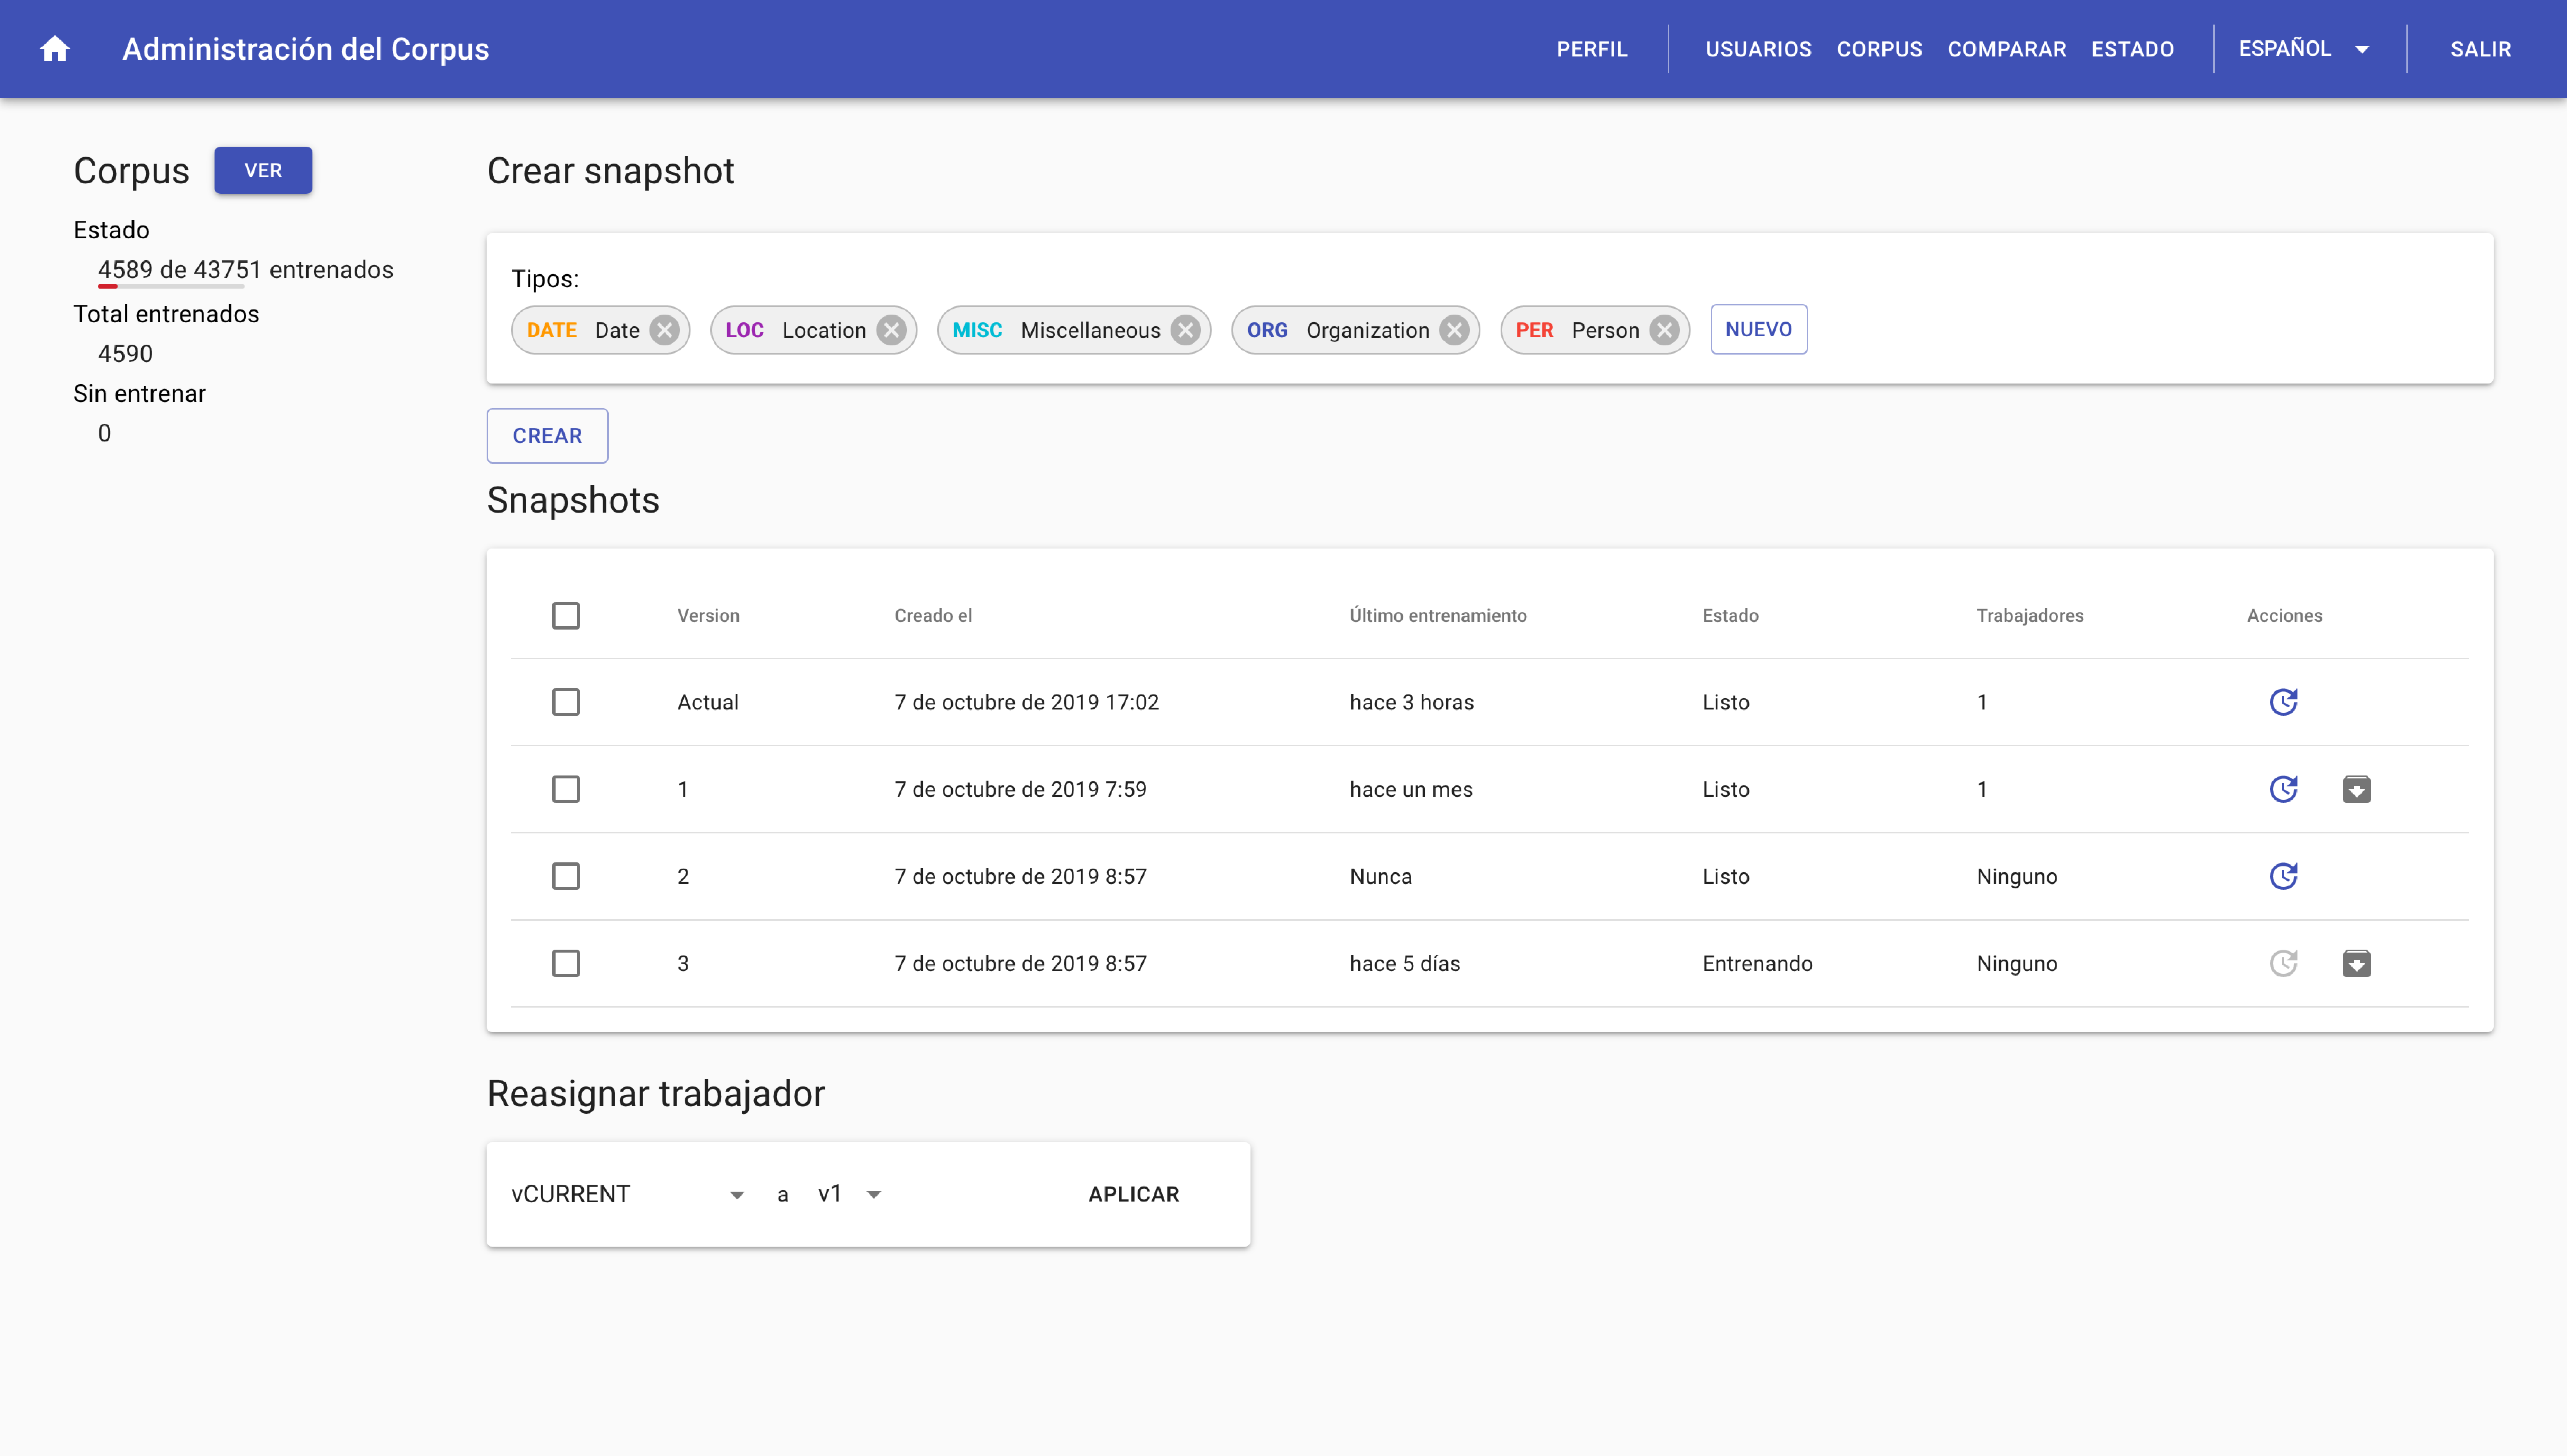
\includegraphics{assets/logic/status.pdf} 

}

\caption{Información de corpus y manejo de workers.}\label{fig:logic-status}
\end{figure}

\hypertarget{secciones}{%
\subparagraph{Secciones}\label{secciones}}

Corpus

Es esta columna a la izquierda se puede ver rápidamente que porcentaje de el \emph{corpus} contiene correcciones por usuarios así como también saber la cantidad total de correcciones del sistema (un texto puede tener más de una corrección por distintos usuarios) y también presenta un botón que permite al administrador ir a la pantalla de \emph{Corpus}.

Crear \emph{snapshot}

En esta sección, el administrador puede crear un \emph{snapshot} del estado actual de entrenamiento del modelo. Esta funcionalidad es utiil para comparar el avance del entrenamiento en diferentes momentos de la historia del mismo.

Cuando se crea un \emph{snapshot} se incrementa la última versión disponible en uno y se gesta una nueva versión actual. Además existe la posibilidad de editar los posibles tipos de entidad del sistema en este momento. Como consecuencia de esto, el sistema se asegura que todo cambio de etiquetas tenga su correspondiente versión.

\emph{Snapshots}

Sección en la cual podemos ver la lista completa de \emph{snapshots}.
Para cada \emph{snapshot}, se muestra cuando fue la última vez que se entrenó así como también cuantos trabajadores tiene asignados. Finalmente es posible desde aquí forzar a entrenar el modelo para ese snapshot en particular y también se presenta la opción para desentrenar, borrando el modelo guardado en el disco.

Cuando el sistema entrena un \emph{snapshot} se tendrá en cuenta todos los textos que hayan sido etiquetados previamente a la creación del mismo.

Reasignar \emph{worker}

Sección que permite reasignar \emph{workers} (los servicios encargados de realizar operaciones de \emph{NLP}) para que sirvan un snapshot distinto. De esta manera se pueden servir distintas versiones del modelo de inferencia para poder realizar pruebas sobre los mismos.

\hypertarget{sandbox}{%
\paragraph{Sandbox}\label{sandbox}}

Se accede a la pantalla de \emph{sandbox} desde el inicio haciendo click en el boton de \enquote{Buscar entidades}; permite a los usuarios ingresar sus textos y obtener las entidades nombradas de los mismos haciendo consultas al servicio NERd del \emph{snapshot} actual.
Adicionalmente, si el usuario tiene el rol de entrenador, podrá corregir las entidades inferidas y agregar el texto con sus correcciones al \emph{corpus} (Figura \ref{fig:logic-sandbox}).

\begin{figure}[H]

{\centering 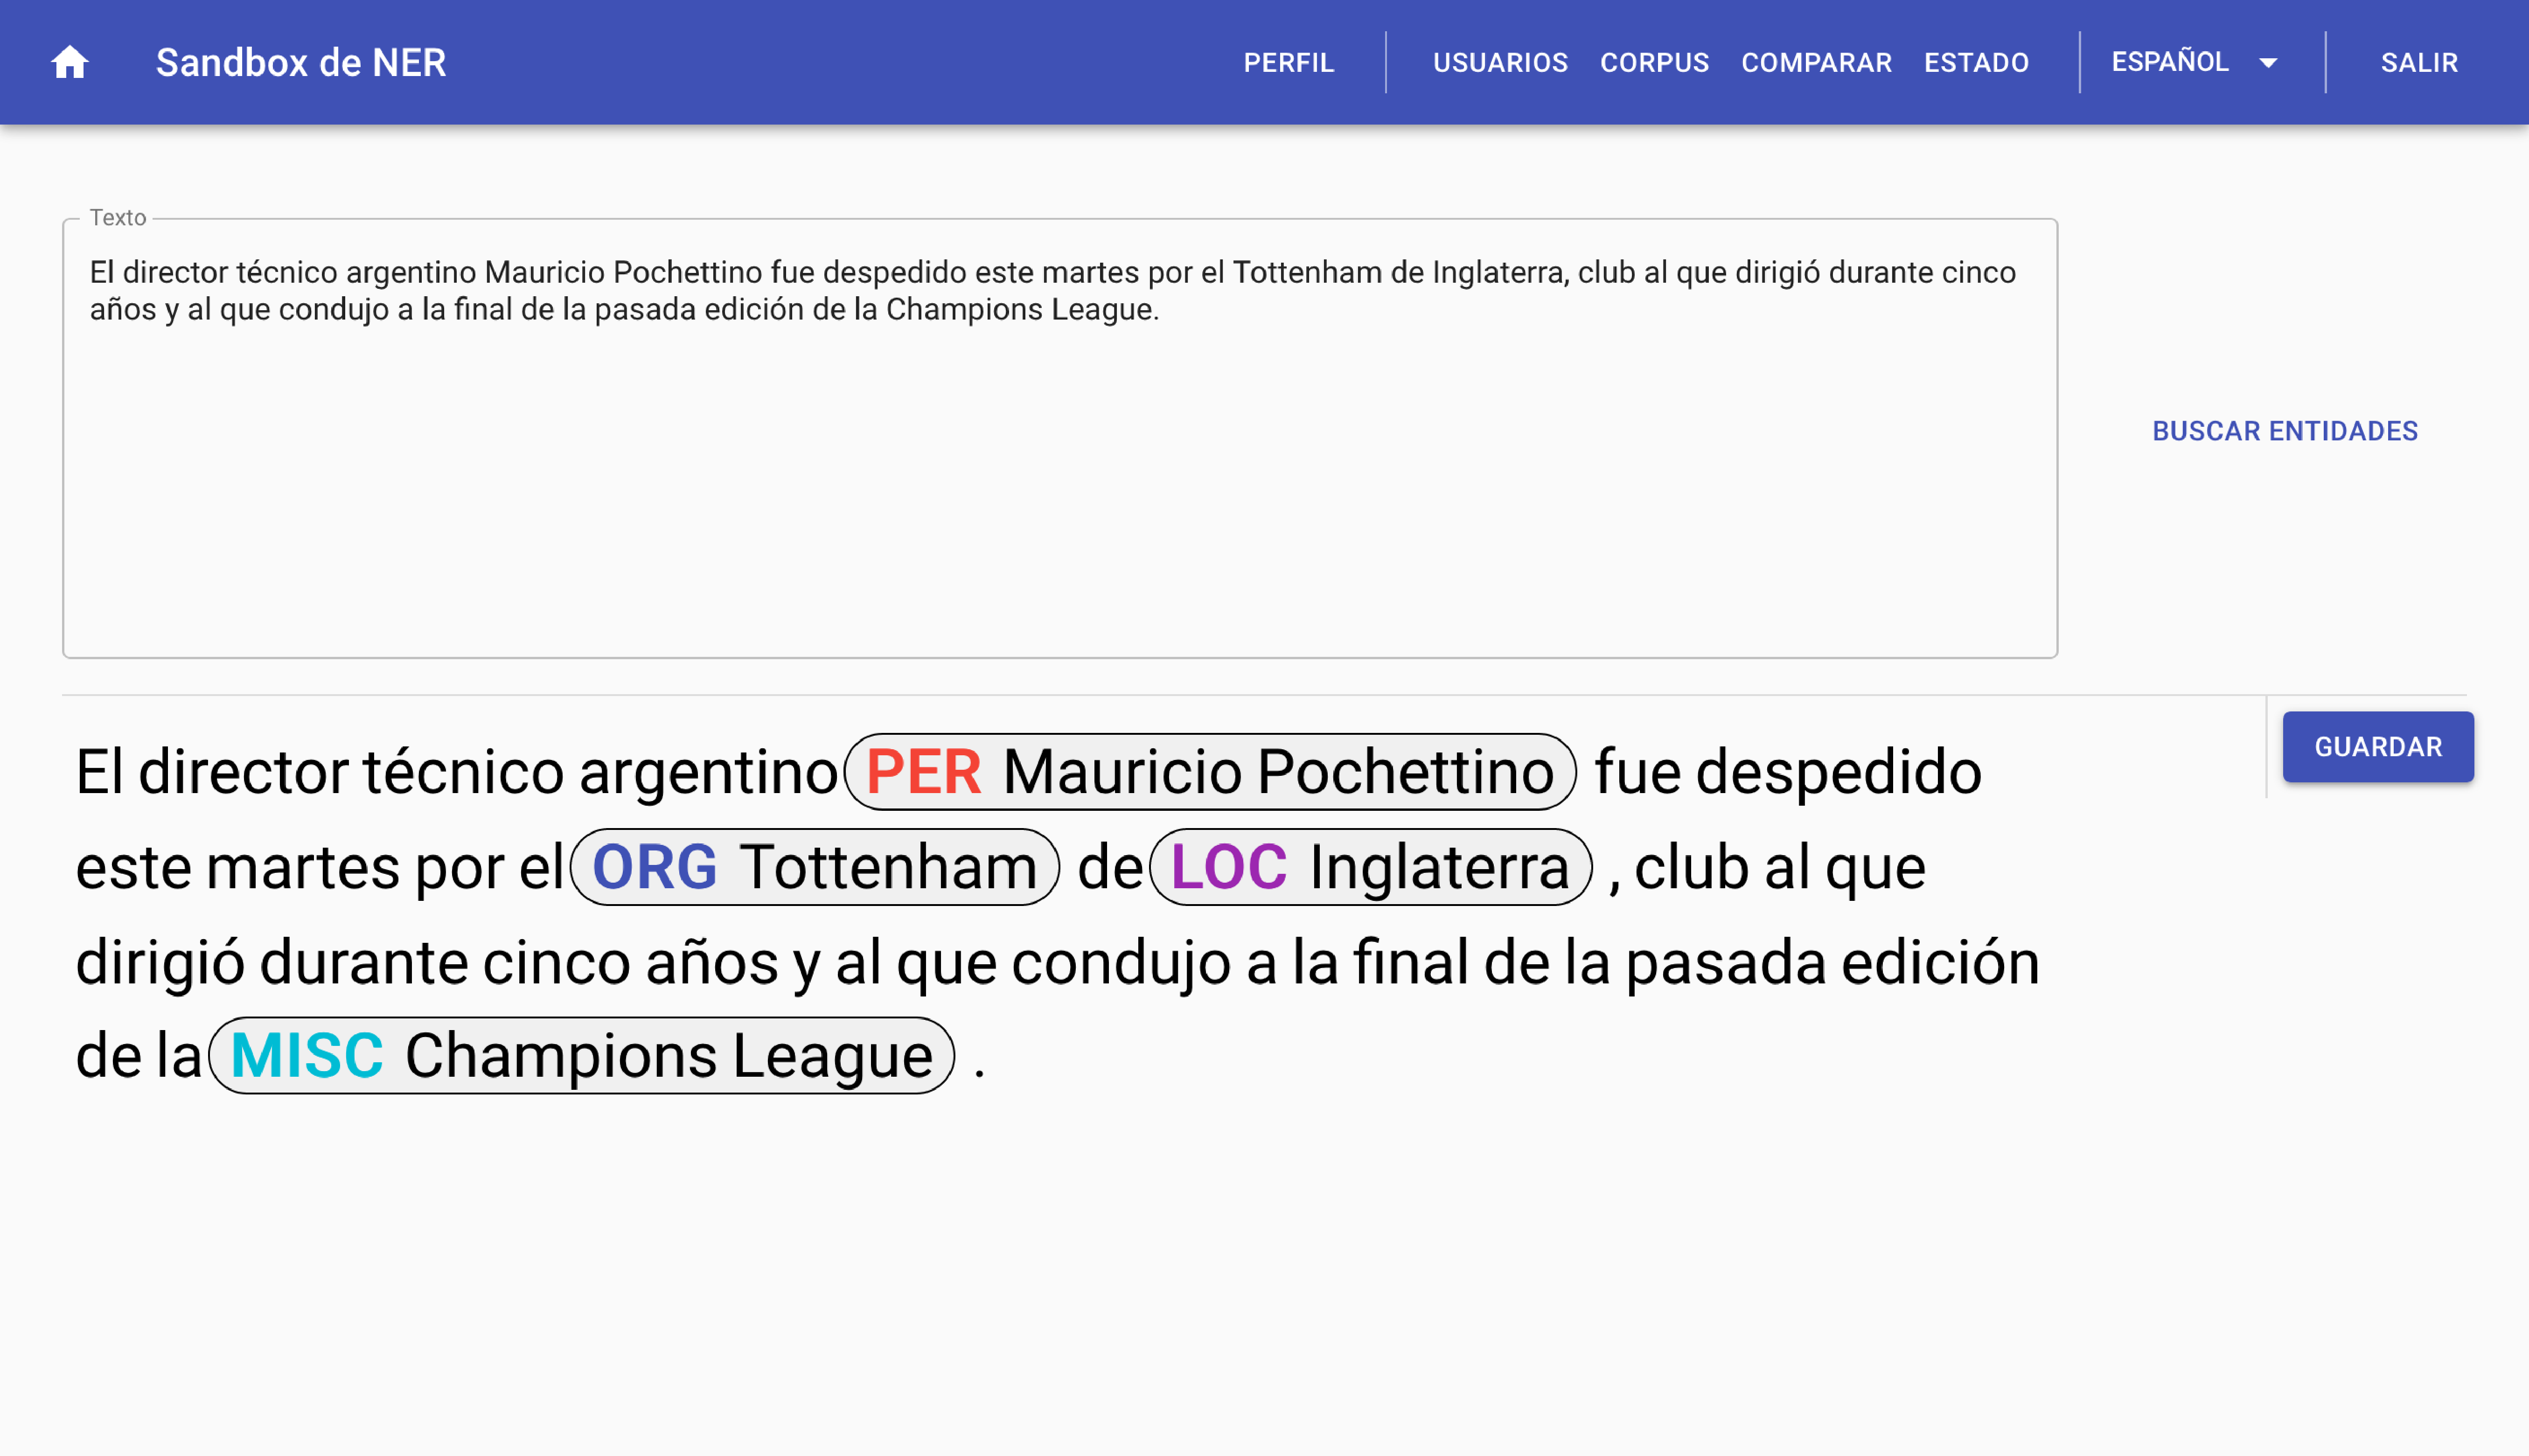
\includegraphics{assets/logic/sandbox.pdf} 

}

\caption{Inferencia de entidades en sandbox.}\label{fig:logic-sandbox}
\end{figure}

\hypertarget{comparar-snapshots}{%
\paragraph{\texorpdfstring{Comparar (\emph{snapshots})}{Comparar (snapshots)}}\label{comparar-snapshots}}

Esta sección es accesible únicamente por administradores y permite comparar las entidades inferidas por dos \emph{snapshots} distintos, con la opción de marcar visualmente aquellos textos cuyas entidades difieren. A su vez, si el usuario logueado tiene el permiso de entrenador, podrá corregir de manera inline los errores en la inferencia del modelo actual (Figura \ref{fig:logic-compare}).

\begin{figure}[H]

{\centering 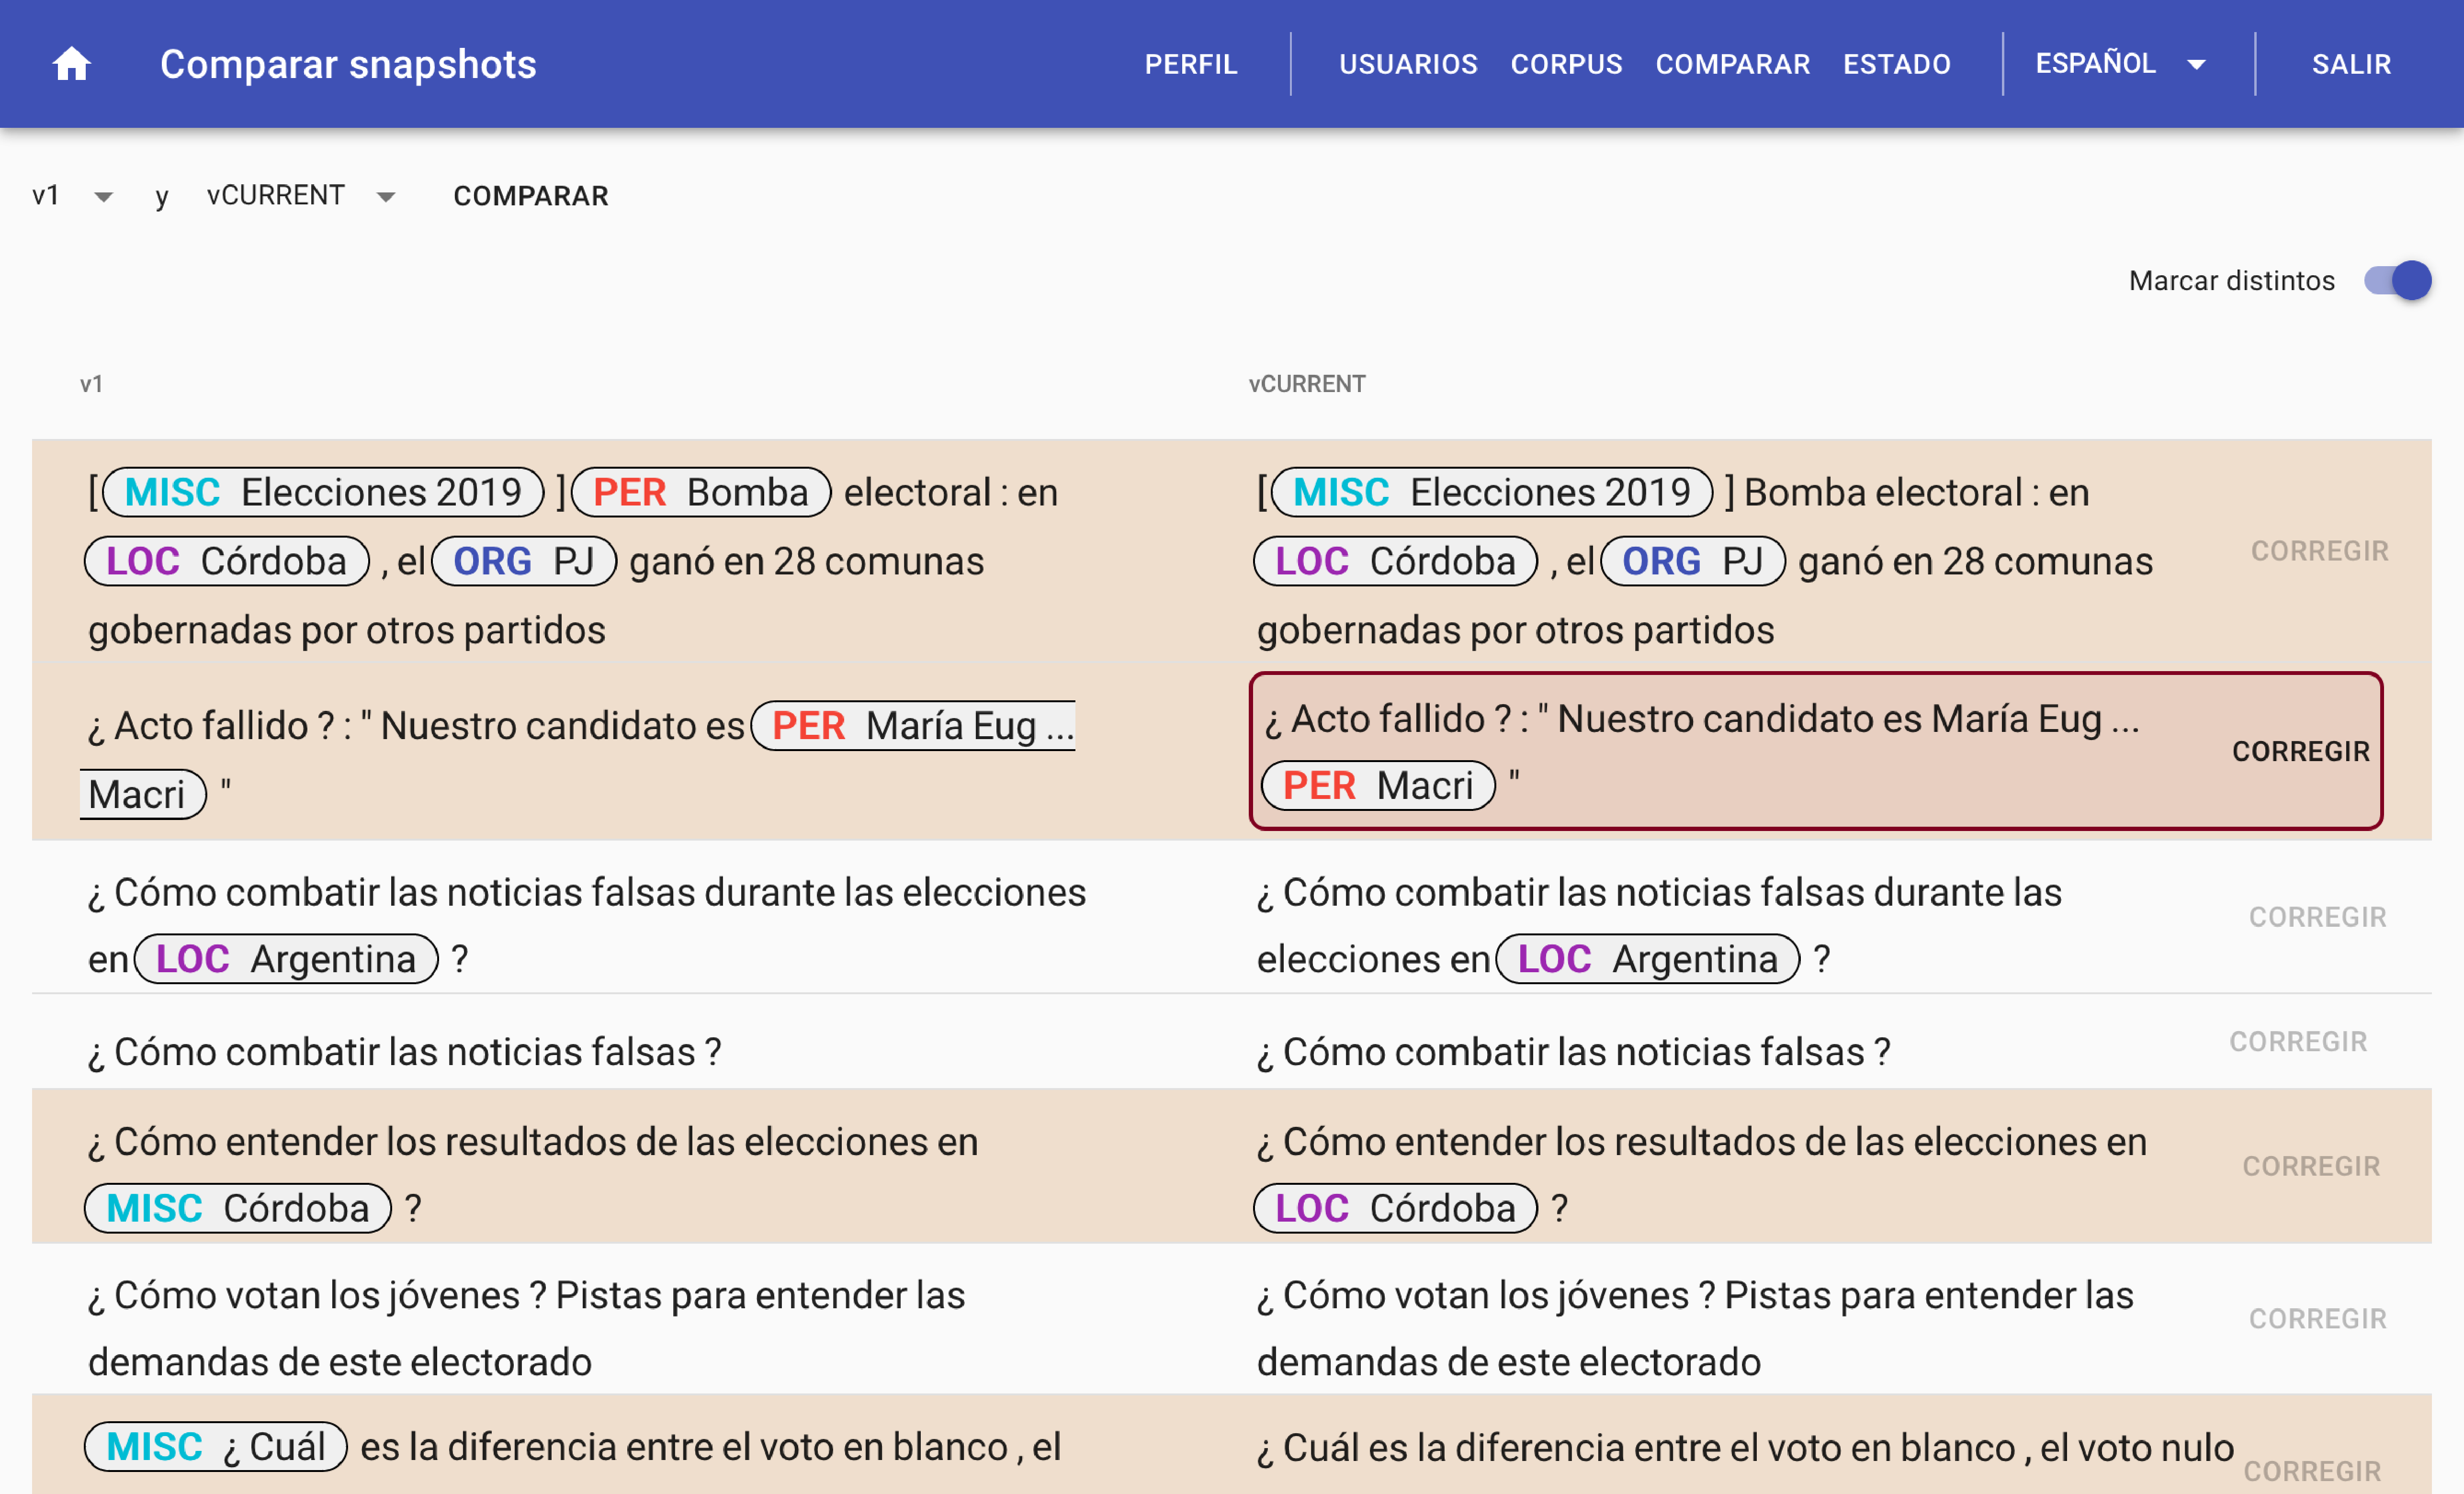
\includegraphics{assets/logic/compare.pdf} 

}

\caption{Comparativa de modelos.}\label{fig:logic-compare}
\end{figure}

\hypertarget{registraciuxf3n}{%
\paragraph{Registración}\label{registraciuxf3n}}

Sección únicamente accesible cuando no hay una sesión activa. Aquí se registran los usuarios con la opción de que el inicio de sesión persista luego de que se cierre la pestaña del navegador (Figura \ref{fig:logic-registration}).

\begin{figure}[H]

{\centering 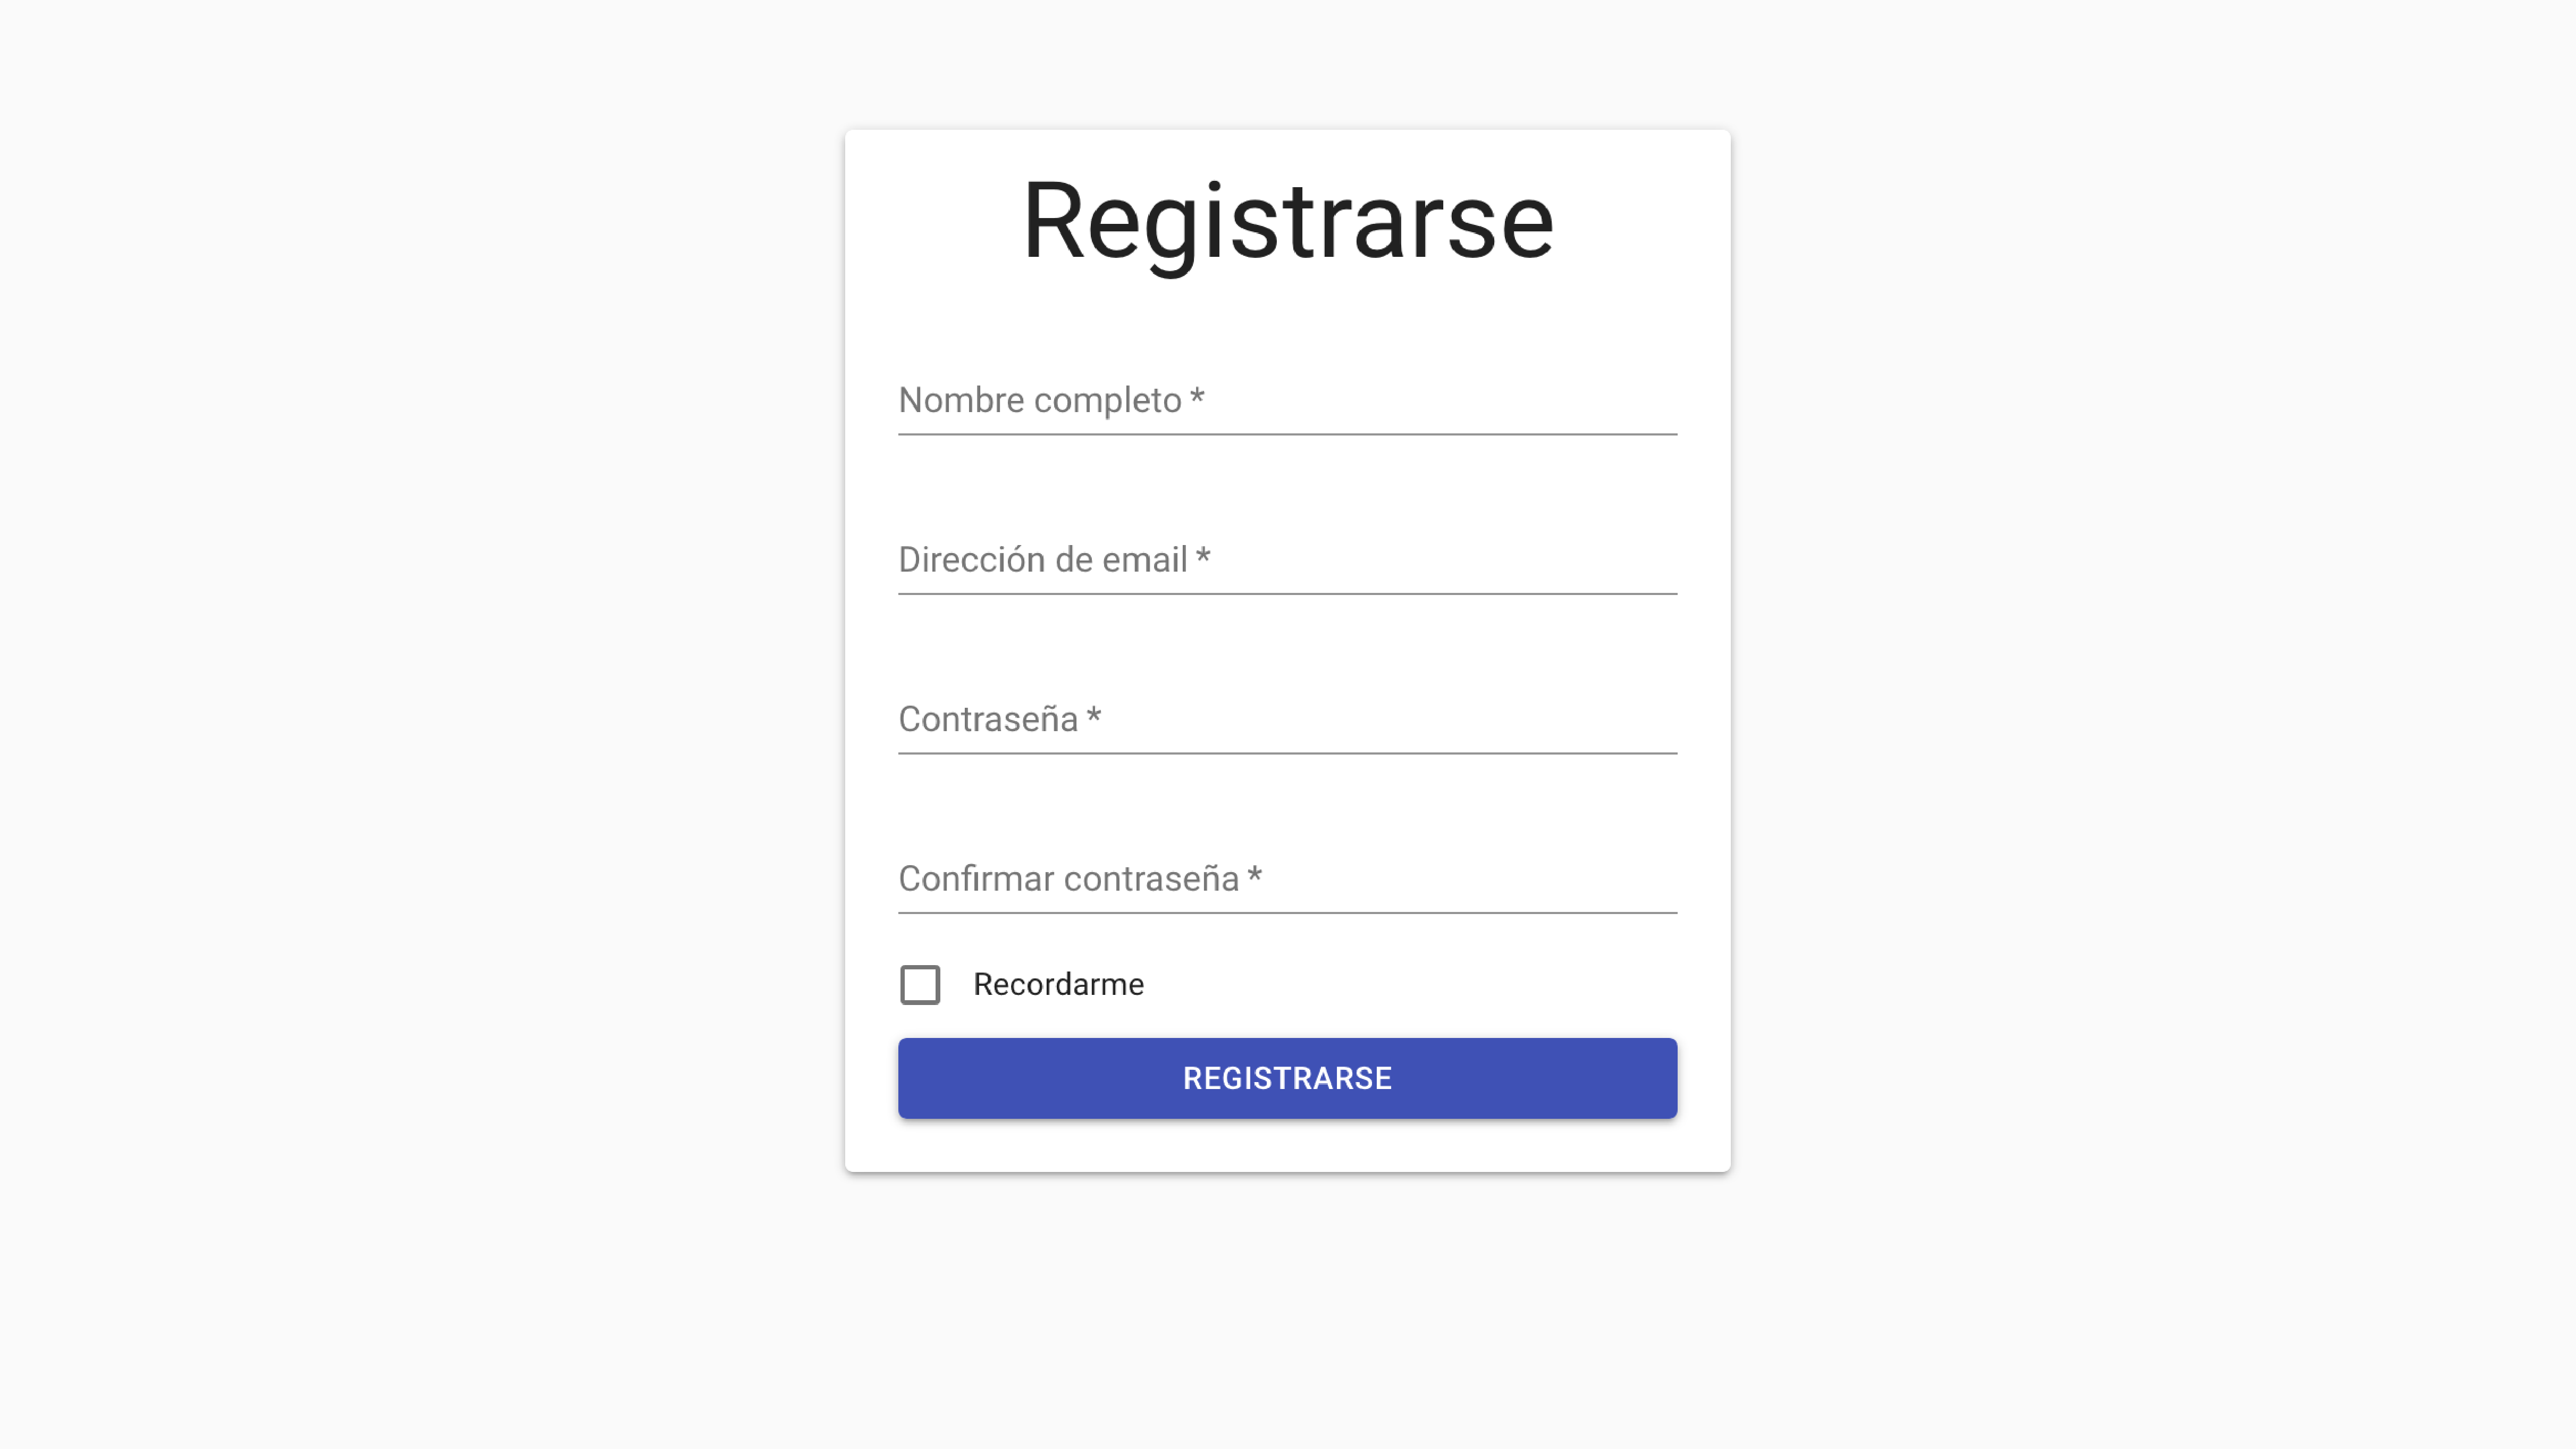
\includegraphics{assets/logic/register.pdf} 

}

\caption{Registración.}\label{fig:logic-registration}
\end{figure}

\hypertarget{login}{%
\paragraph{Login}\label{login}}

Sección únicamente accesible cuando no hay una sesión activa. Aquí ingresan los usuarios al sistema con la opción de que el inicio de sesión persista luego de que se cierre la pestaña del navegador (Figura \ref{fig:logic-login}).

\begin{figure}[H]

{\centering 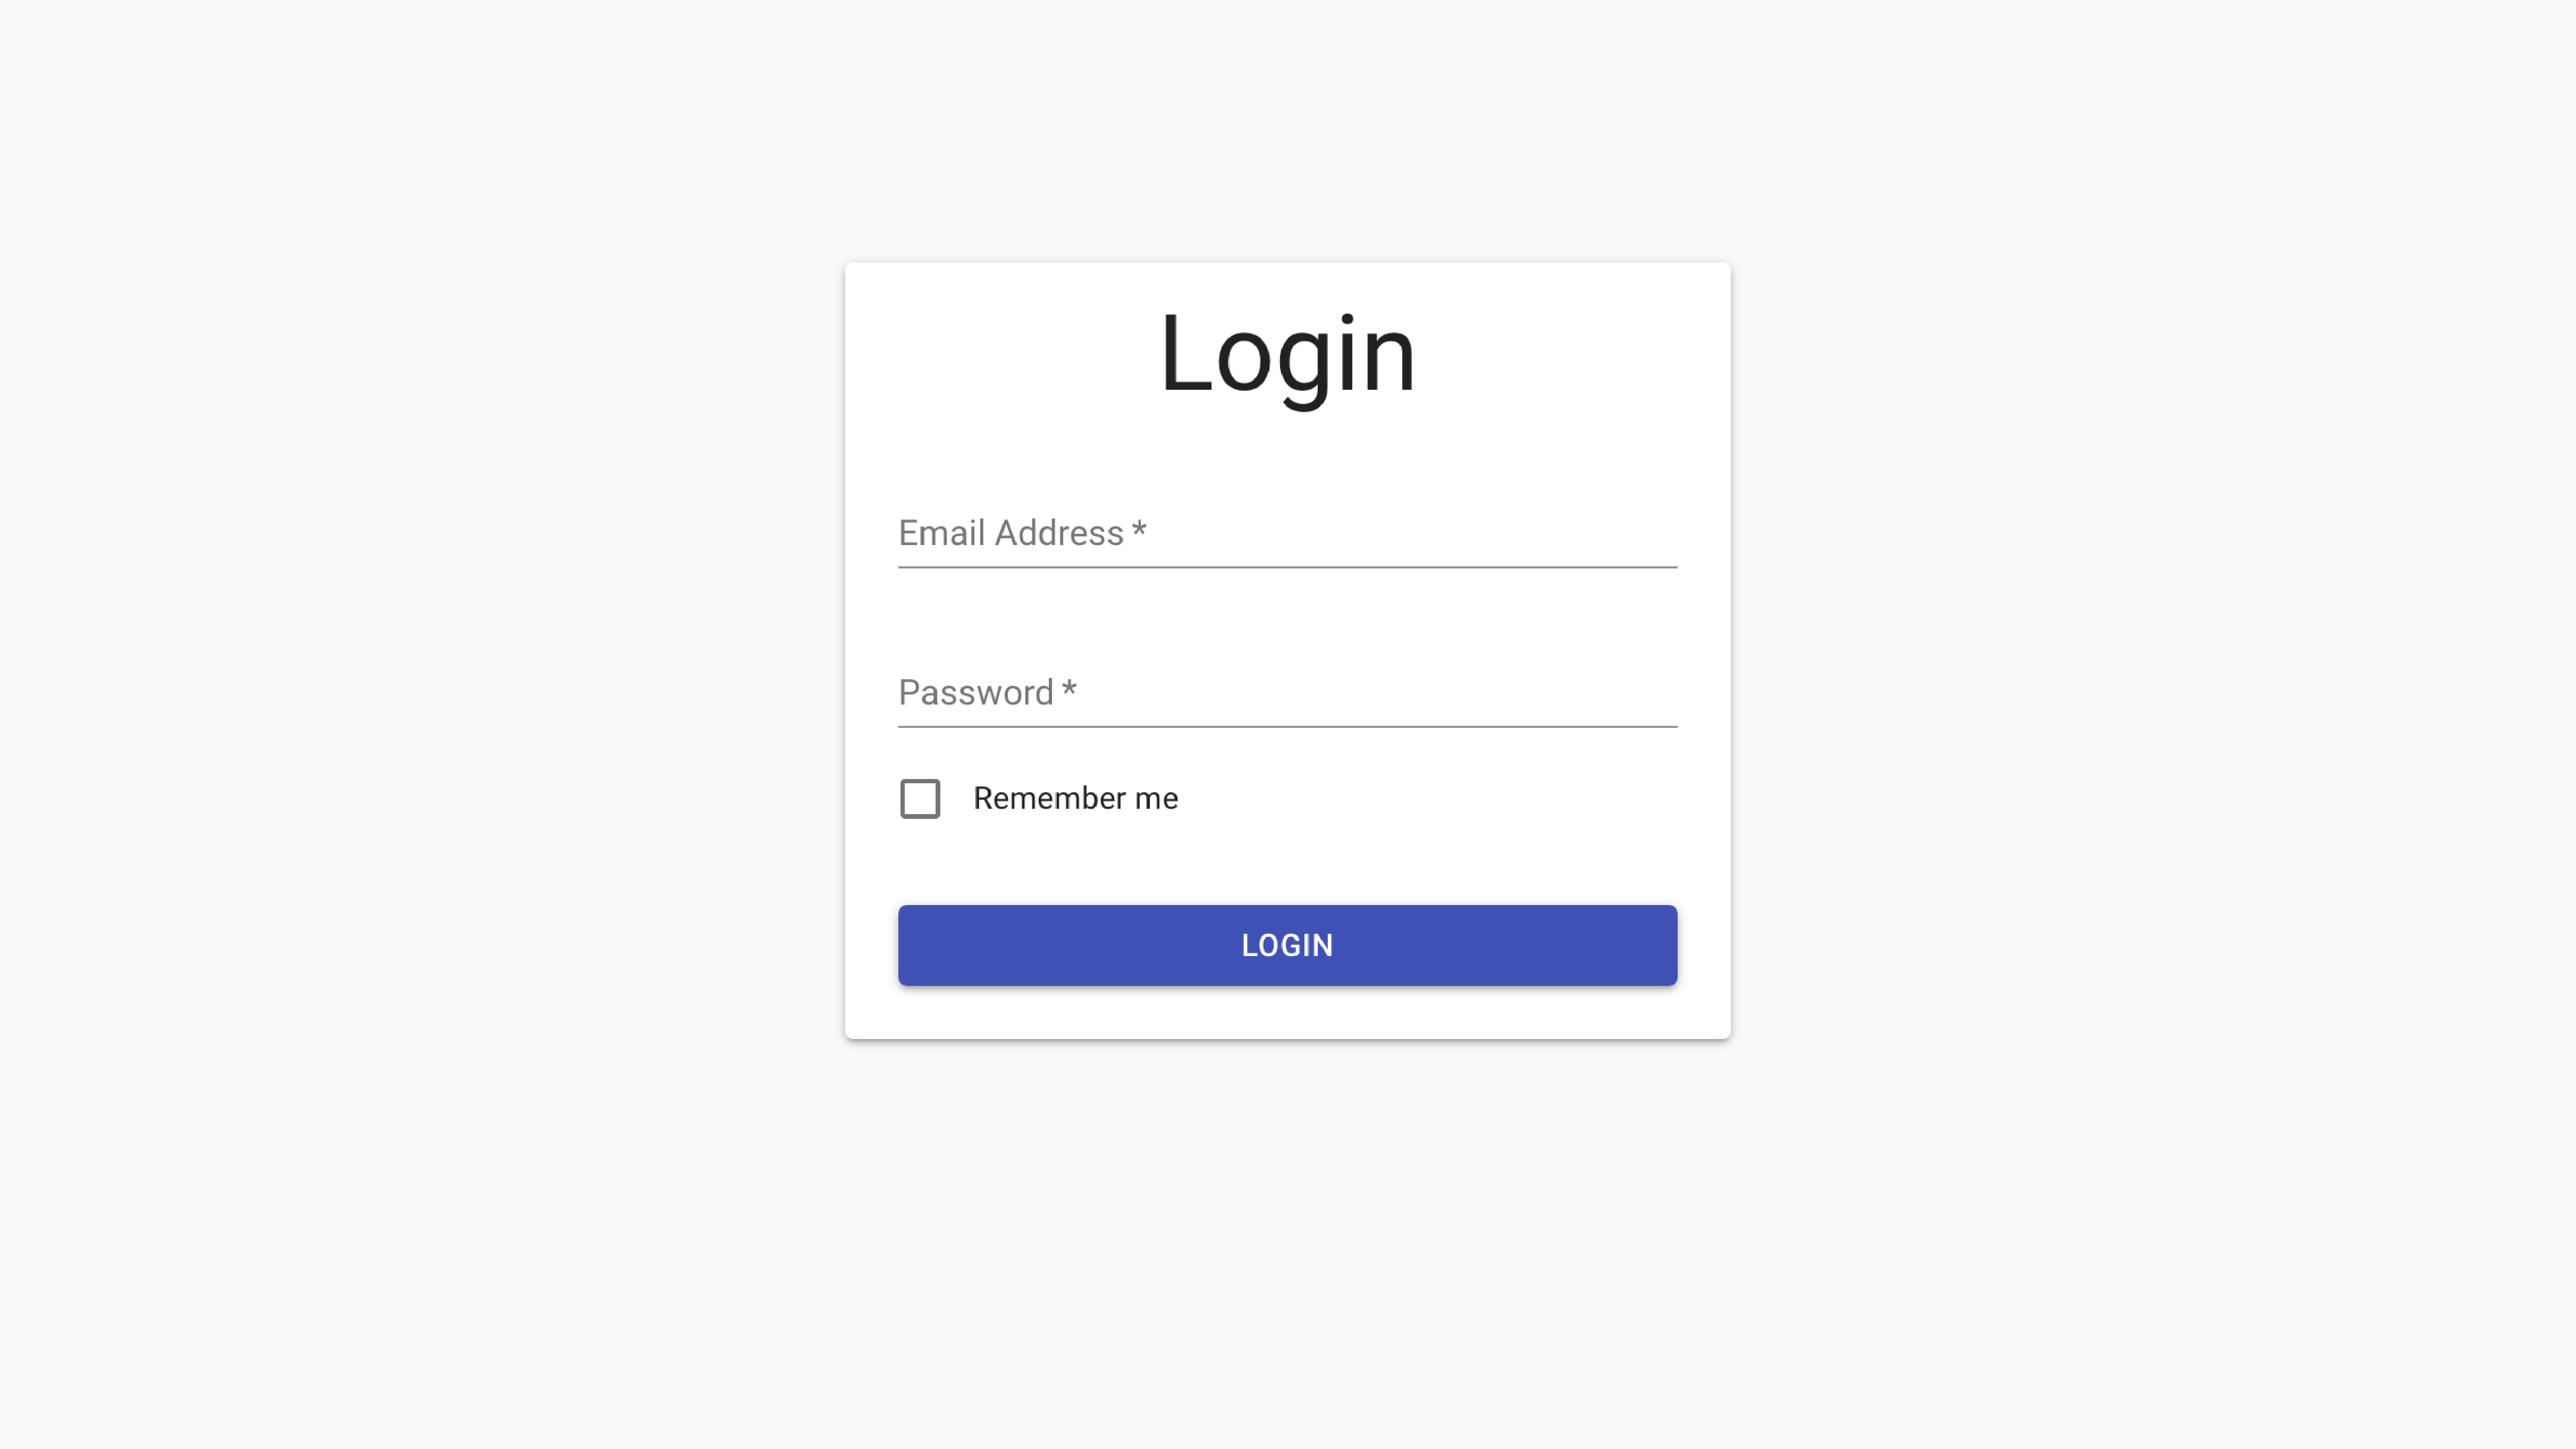
\includegraphics{assets/logic/login.pdf} 

}

\caption{Inicio de sesión.}\label{fig:logic-login}
\end{figure}

\hypertarget{barra-de-navegaciuxf3n}{%
\paragraph{Barra de navegación}\label{barra-de-navegaciuxf3n}}

La barra de navegación muestra distinta información dependiendo del contexto actual del sistema.

Cuando no hay una sesión activa, se muestran únicamente las opciones para acceder al sistema, ya sea registrándose o ingresando utilizando credenciales (Figura \ref{fig:logic-status-anonymous}).

\begin{figure}[H]

{\centering 
\includegraphics{assets/logic/status-anonymous.pdf} 

}

\caption{Usuario anónimo.}\label{fig:logic-status-anonymous}
\end{figure}

Cuando hay una sesión activa el usuario cuenta con el rol de \emph{USER} y/o de \emph{TRAINER} pero \textbf{no} con el de \emph{ADMIN}, podrá acceder únicamente a su perfil (Figura \ref{fig:logic-status-user}).

\begin{figure}[H]

{\centering 
\includegraphics{assets/logic/status-user.pdf} 

}

\caption{Usuario regular.}\label{fig:logic-status-user}
\end{figure}

Finalmente, cuando el usuario logueado tiene el rol de \emph{ADMIN}, tiene acceso a todas las secciones de administración del sistema (Figura \ref(fig:logic-status-admin)).

\begin{figure}[H]

{\centering 
\includegraphics{assets/logic/status-admin.pdf} 

}

\caption{Usuario administrador.}\label{fig:logic-status-admin}
\end{figure}

\hypertarget{api}{%
\subsubsection{\texorpdfstring{\emph{API}}{API}}\label{api}}

Para este proyecto tomamos la decisión de ofrecer una \emph{API REST}. Dado que \emph{REST} es un estilo de arquitectura y \textbf{no un standard} históricamente ha sido dificil ofrecer este tipo de servicio de una manera amena para el developer.

En los últimos años han surgido especificaciones bien formadas para la definición de \emph{REST APIs}, en particular \emph{The Linux Foundation} ha promovido que la industria utilice \emph{OPEN API}.

Es por ello que toda la especificación de nuestra \emph{API} es \emph{OpenAPI 3} compliant.

\hypertarget{documentaciuxf3n}{%
\paragraph{Documentación}\label{documentaciuxf3n}}

Para visualizar la documentación de todos los \emph{endpoints} del \emph{API}, es posible utilizar dos medios: \emph{Swagger UI} y \emph{ReDoc}. Gracias al uso de \emph{OpenAPI} estas documentaciones han sido autogeneradas.

\hypertarget{swagger-ui}{%
\subparagraph{\texorpdfstring{\emph{Swagger UI}}{Swagger UI}}\label{swagger-ui}}

La documentación provista por \emph{Swagger UI} permite ver el detalle de cada uno de los \emph{endpoints} del servicio así como también permite realizar consultas de prueba contra el servidor real, prestándose así como una especie de \emph{sandbox} (Figura \ref{fig:logic-swagger-main}).

\begin{figure}[H]

{\centering 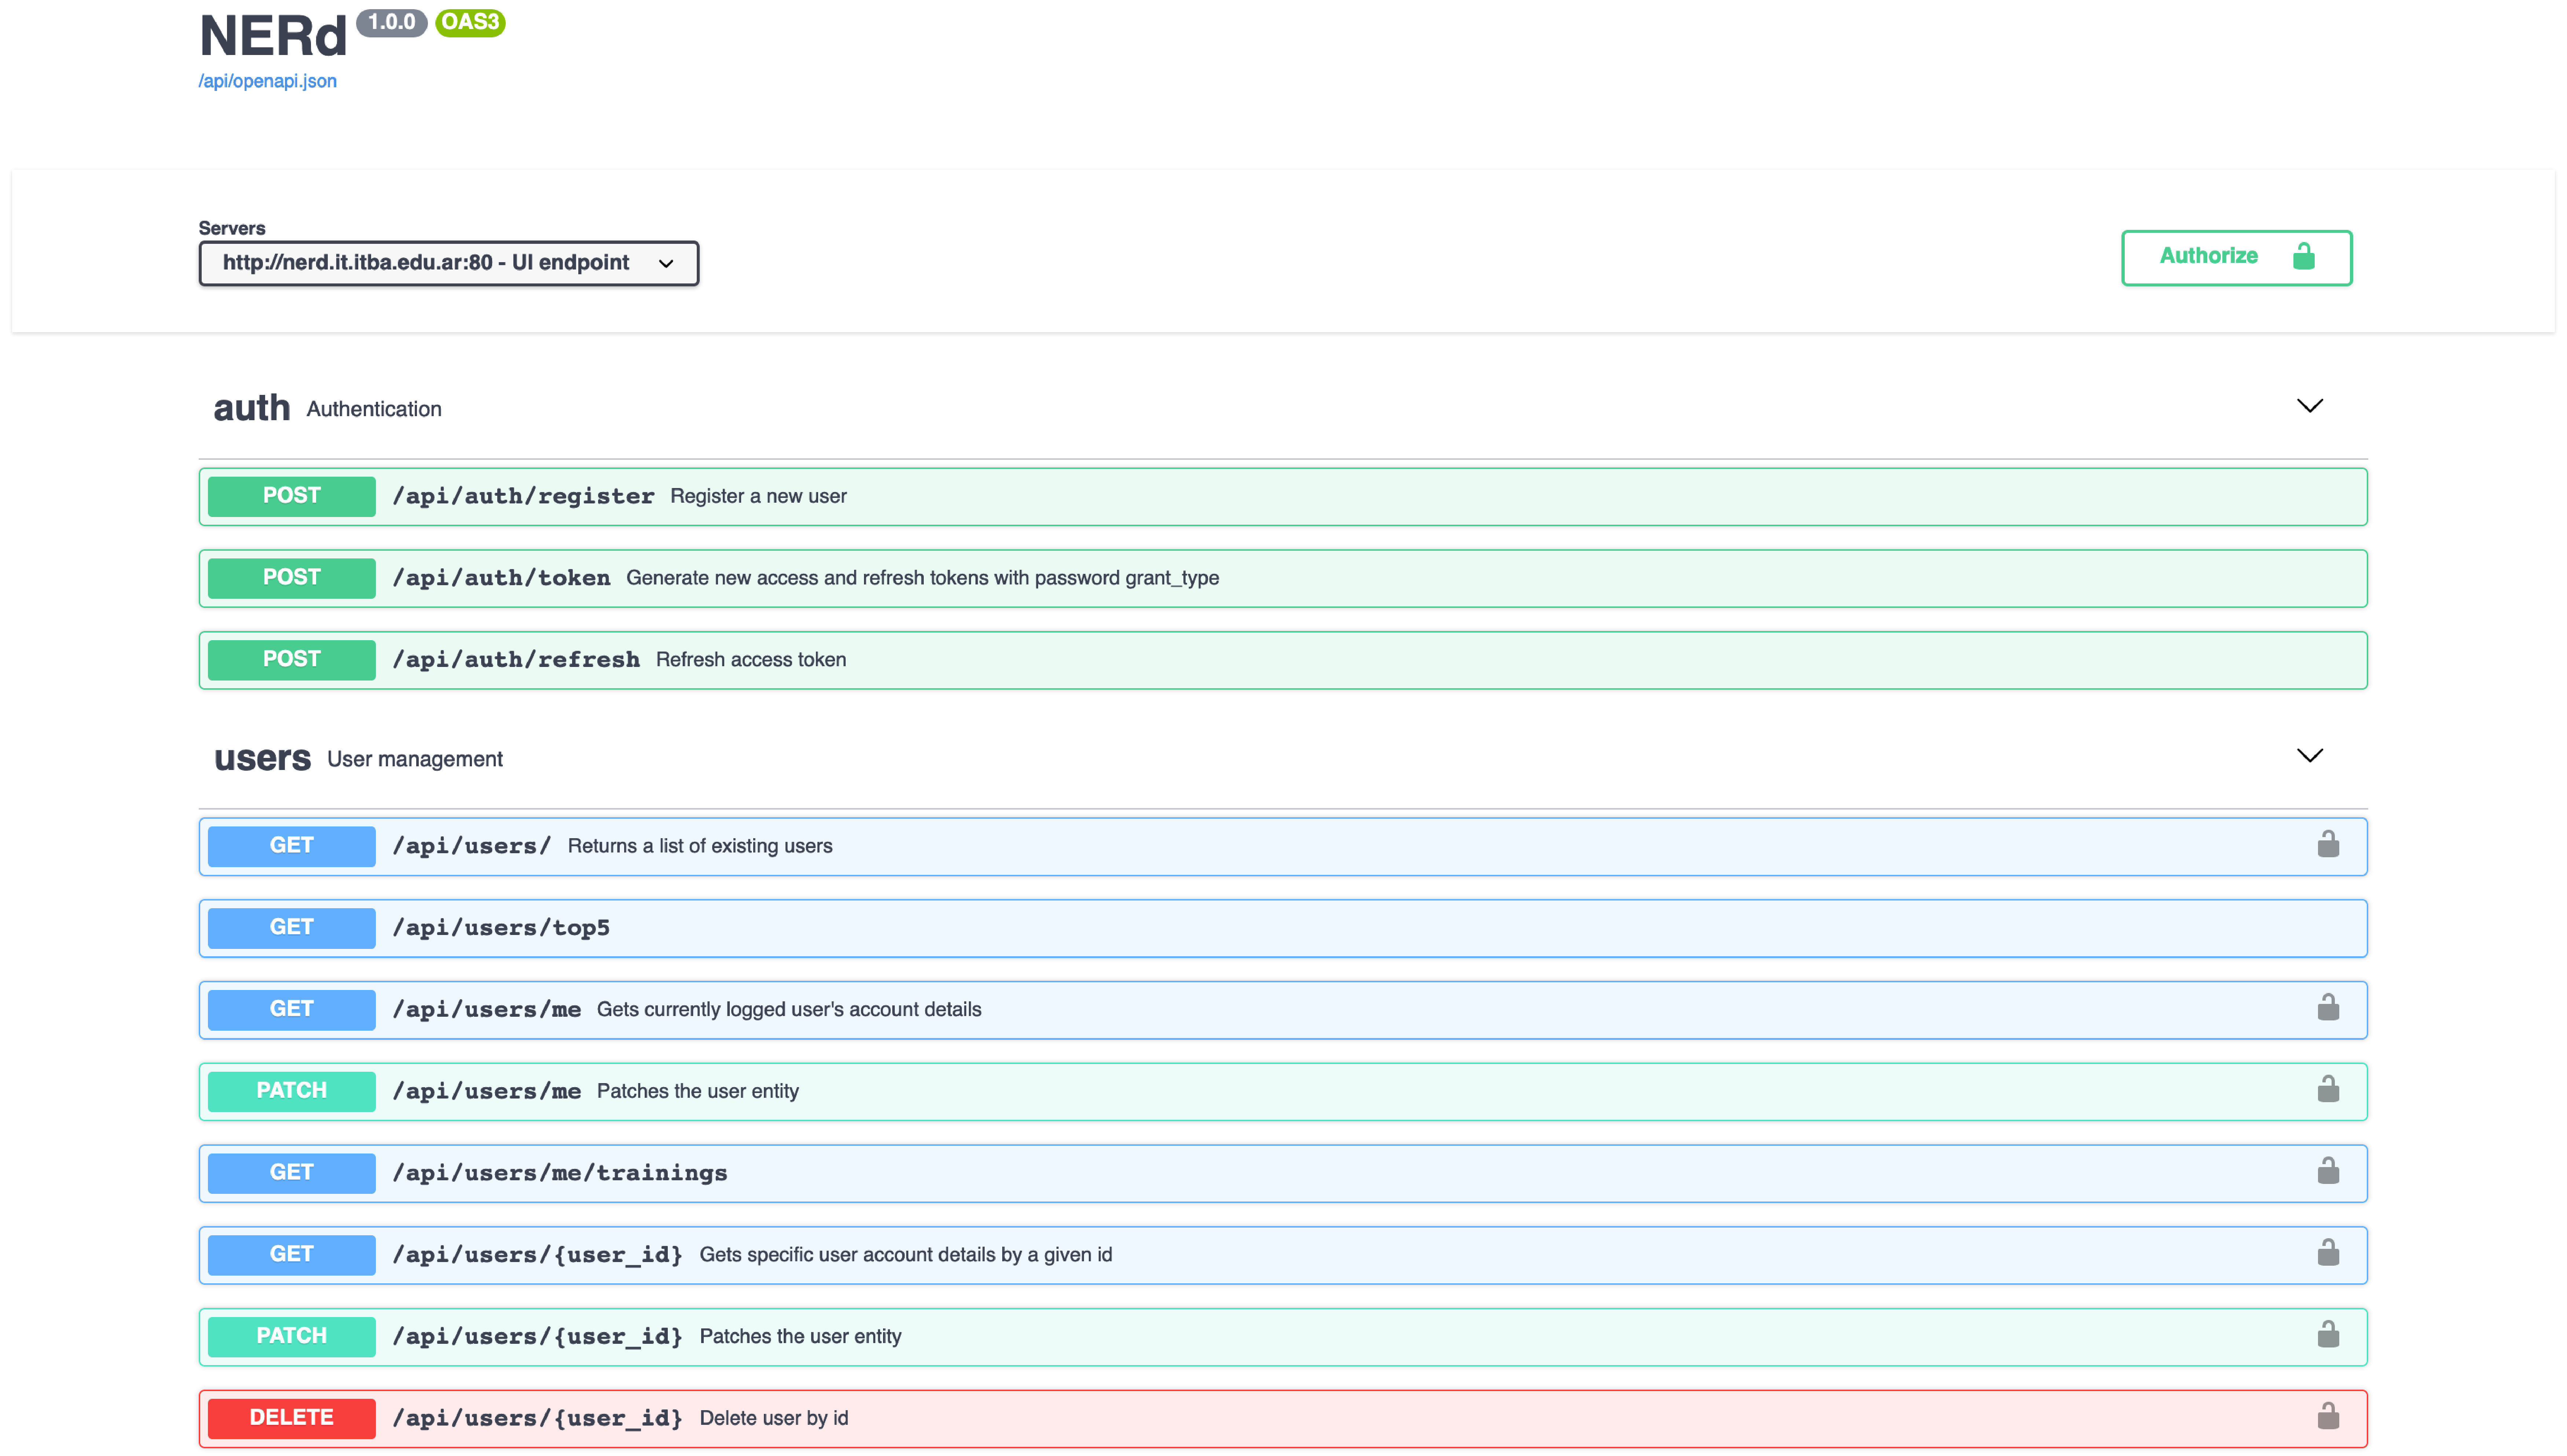
\includegraphics{assets/logic/swagger-main.pdf} 

}

\caption{Swagger UI.}\label{fig:logic-swagger-main}
\end{figure}

Para cada \emph{endpoint}, la interfaz muestra que parámetros son requeridos (Figura \ref{fig:logic-swagger-request}). Así como también permite, mediante el uso del botón \emph{Try it out}, completar esos parámetros y ejecutar el pedido al servidor, mostrando los resultados dentro de la interfaz.

\begin{figure}[H]

{\centering 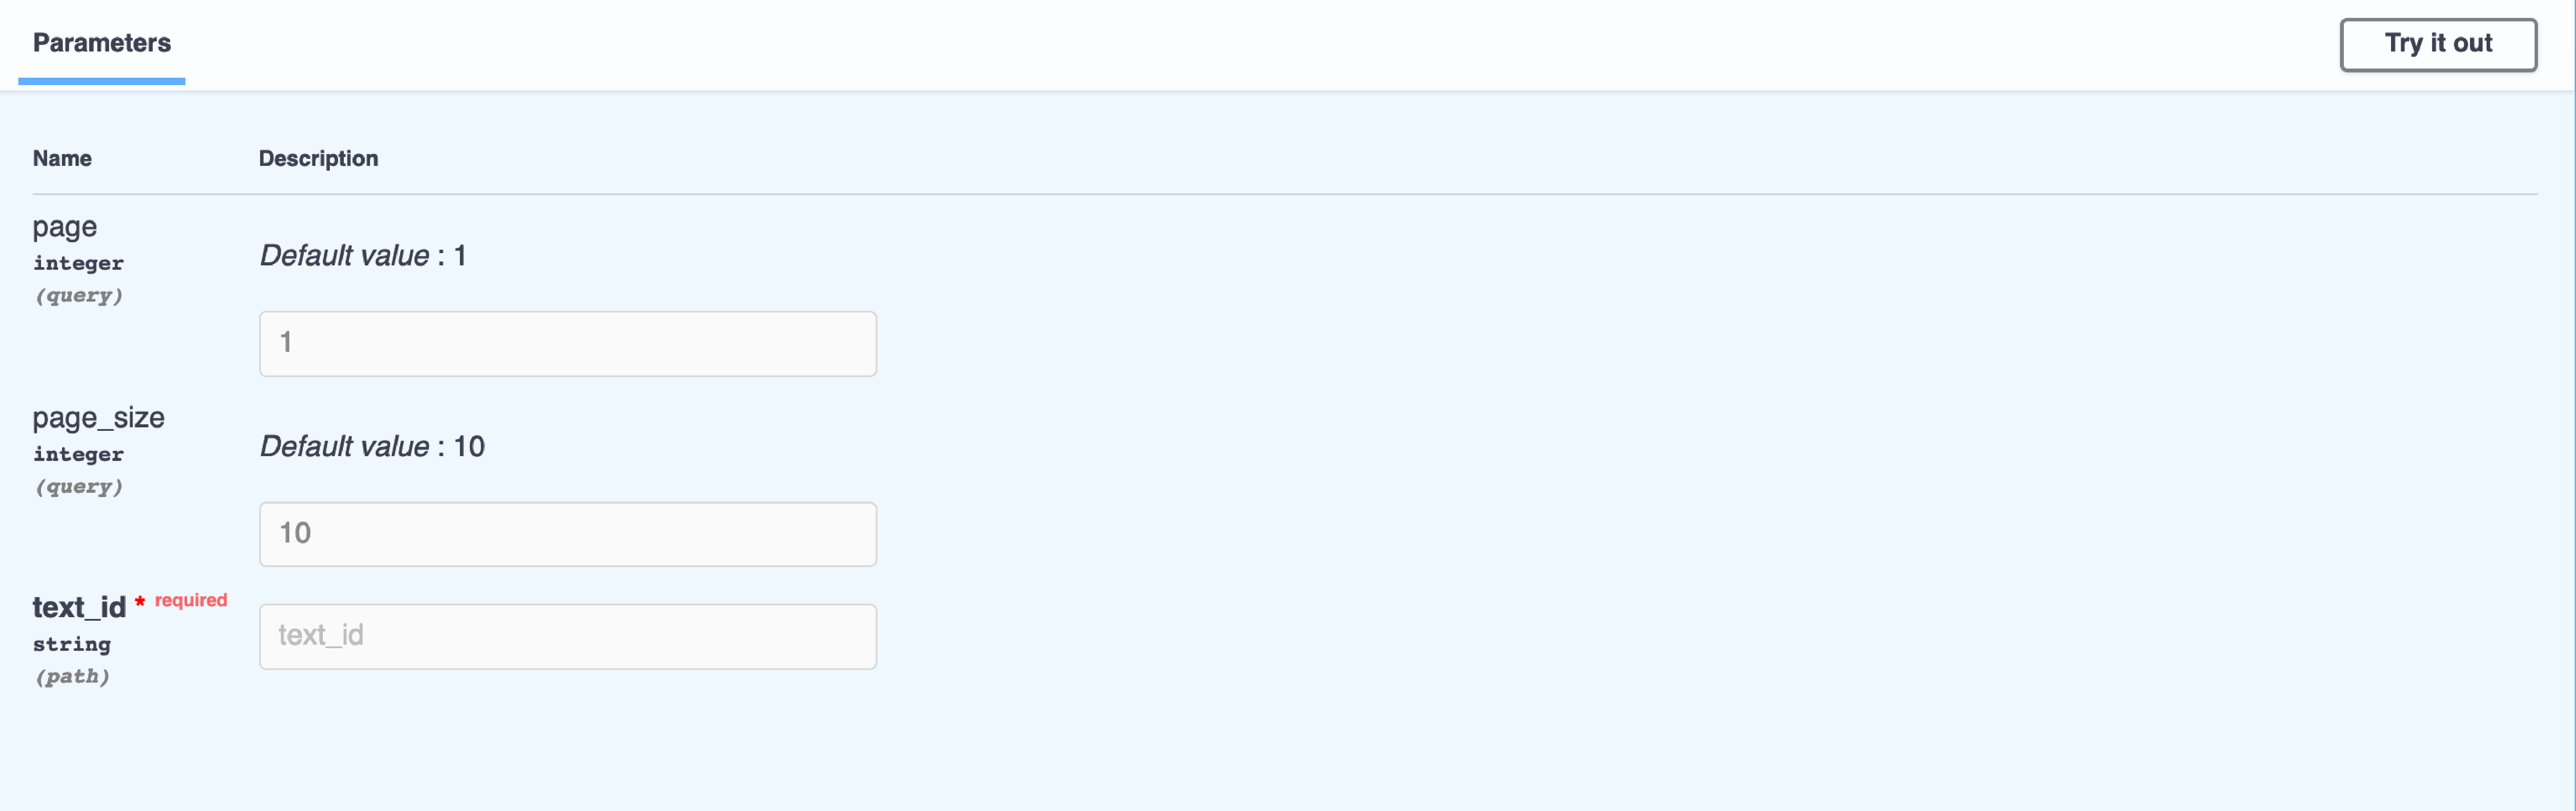
\includegraphics{assets/logic/swagger-request.pdf} 

}

\caption{Ejemplo de documentación con Swagger para request.}\label{fig:logic-swagger-request}
\end{figure}

Para las respuesta, \emph{Swagger} muestra la forma del \emph{JSON} de respuesta para cada \emph{HTTP code} distinto (Figura \ref{fig:logic-swagger-request})

\begin{figure}[H]

{\centering 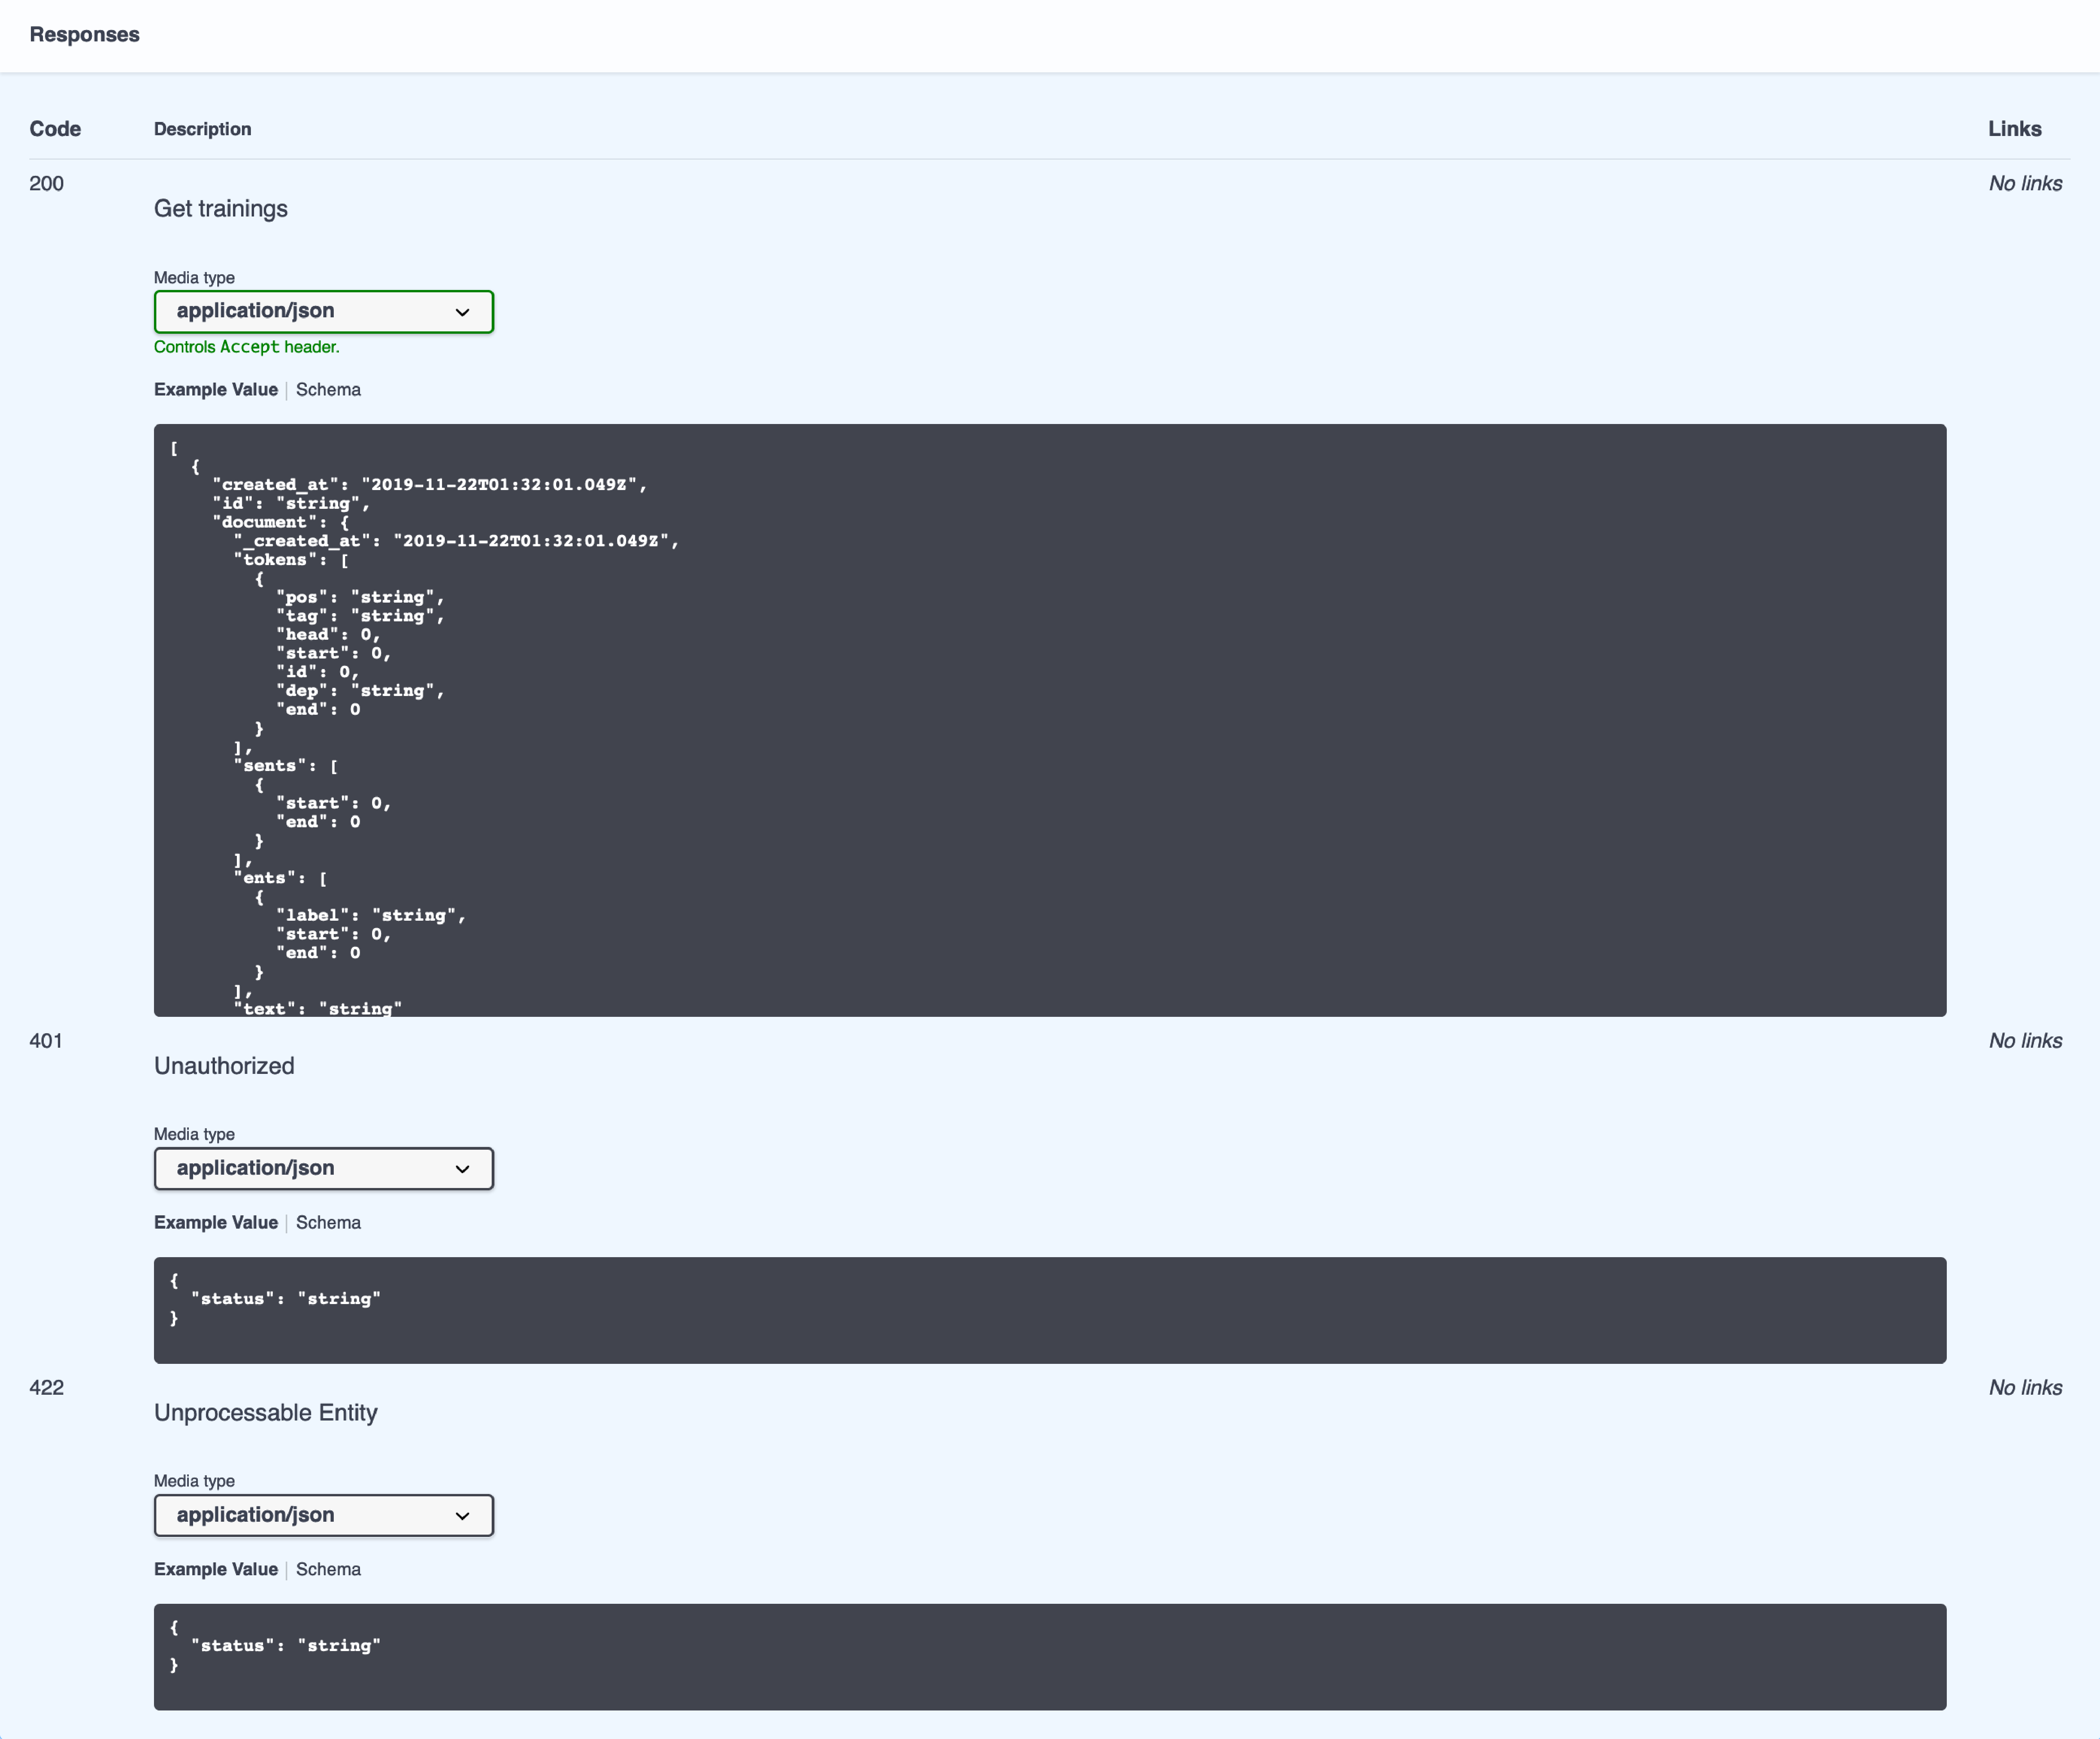
\includegraphics{assets/logic/swagger-responses.pdf} 

}

\caption{Ejemplo de documentación con Swagger para respuestas.}\label{fig:logic-swagger-responses}
\end{figure}

\hypertarget{redoc}{%
\subparagraph{\texorpdfstring{\emph{ReDoc}}{ReDoc}}\label{redoc}}

\emph{ReDoc} es una alternativa a \emph{Swagger} para visualizar la documentación de una especificación de \emph{OpenAPI} que presenta un diseño más moderno así como también se enfoca más en mostrar la información de manera más clara.

A diferencia de \emph{Swagger UI}, \emph{ReDoc} no permite realizar pruebas contra el servidor para el cual se está mostrando la documentación (Figura \ref{fig:logic-redoc-main}) pero ofrece una mejor experiencia de usuario a la hora de navegar la \emph{API}.

\begin{figure}[H]

{\centering 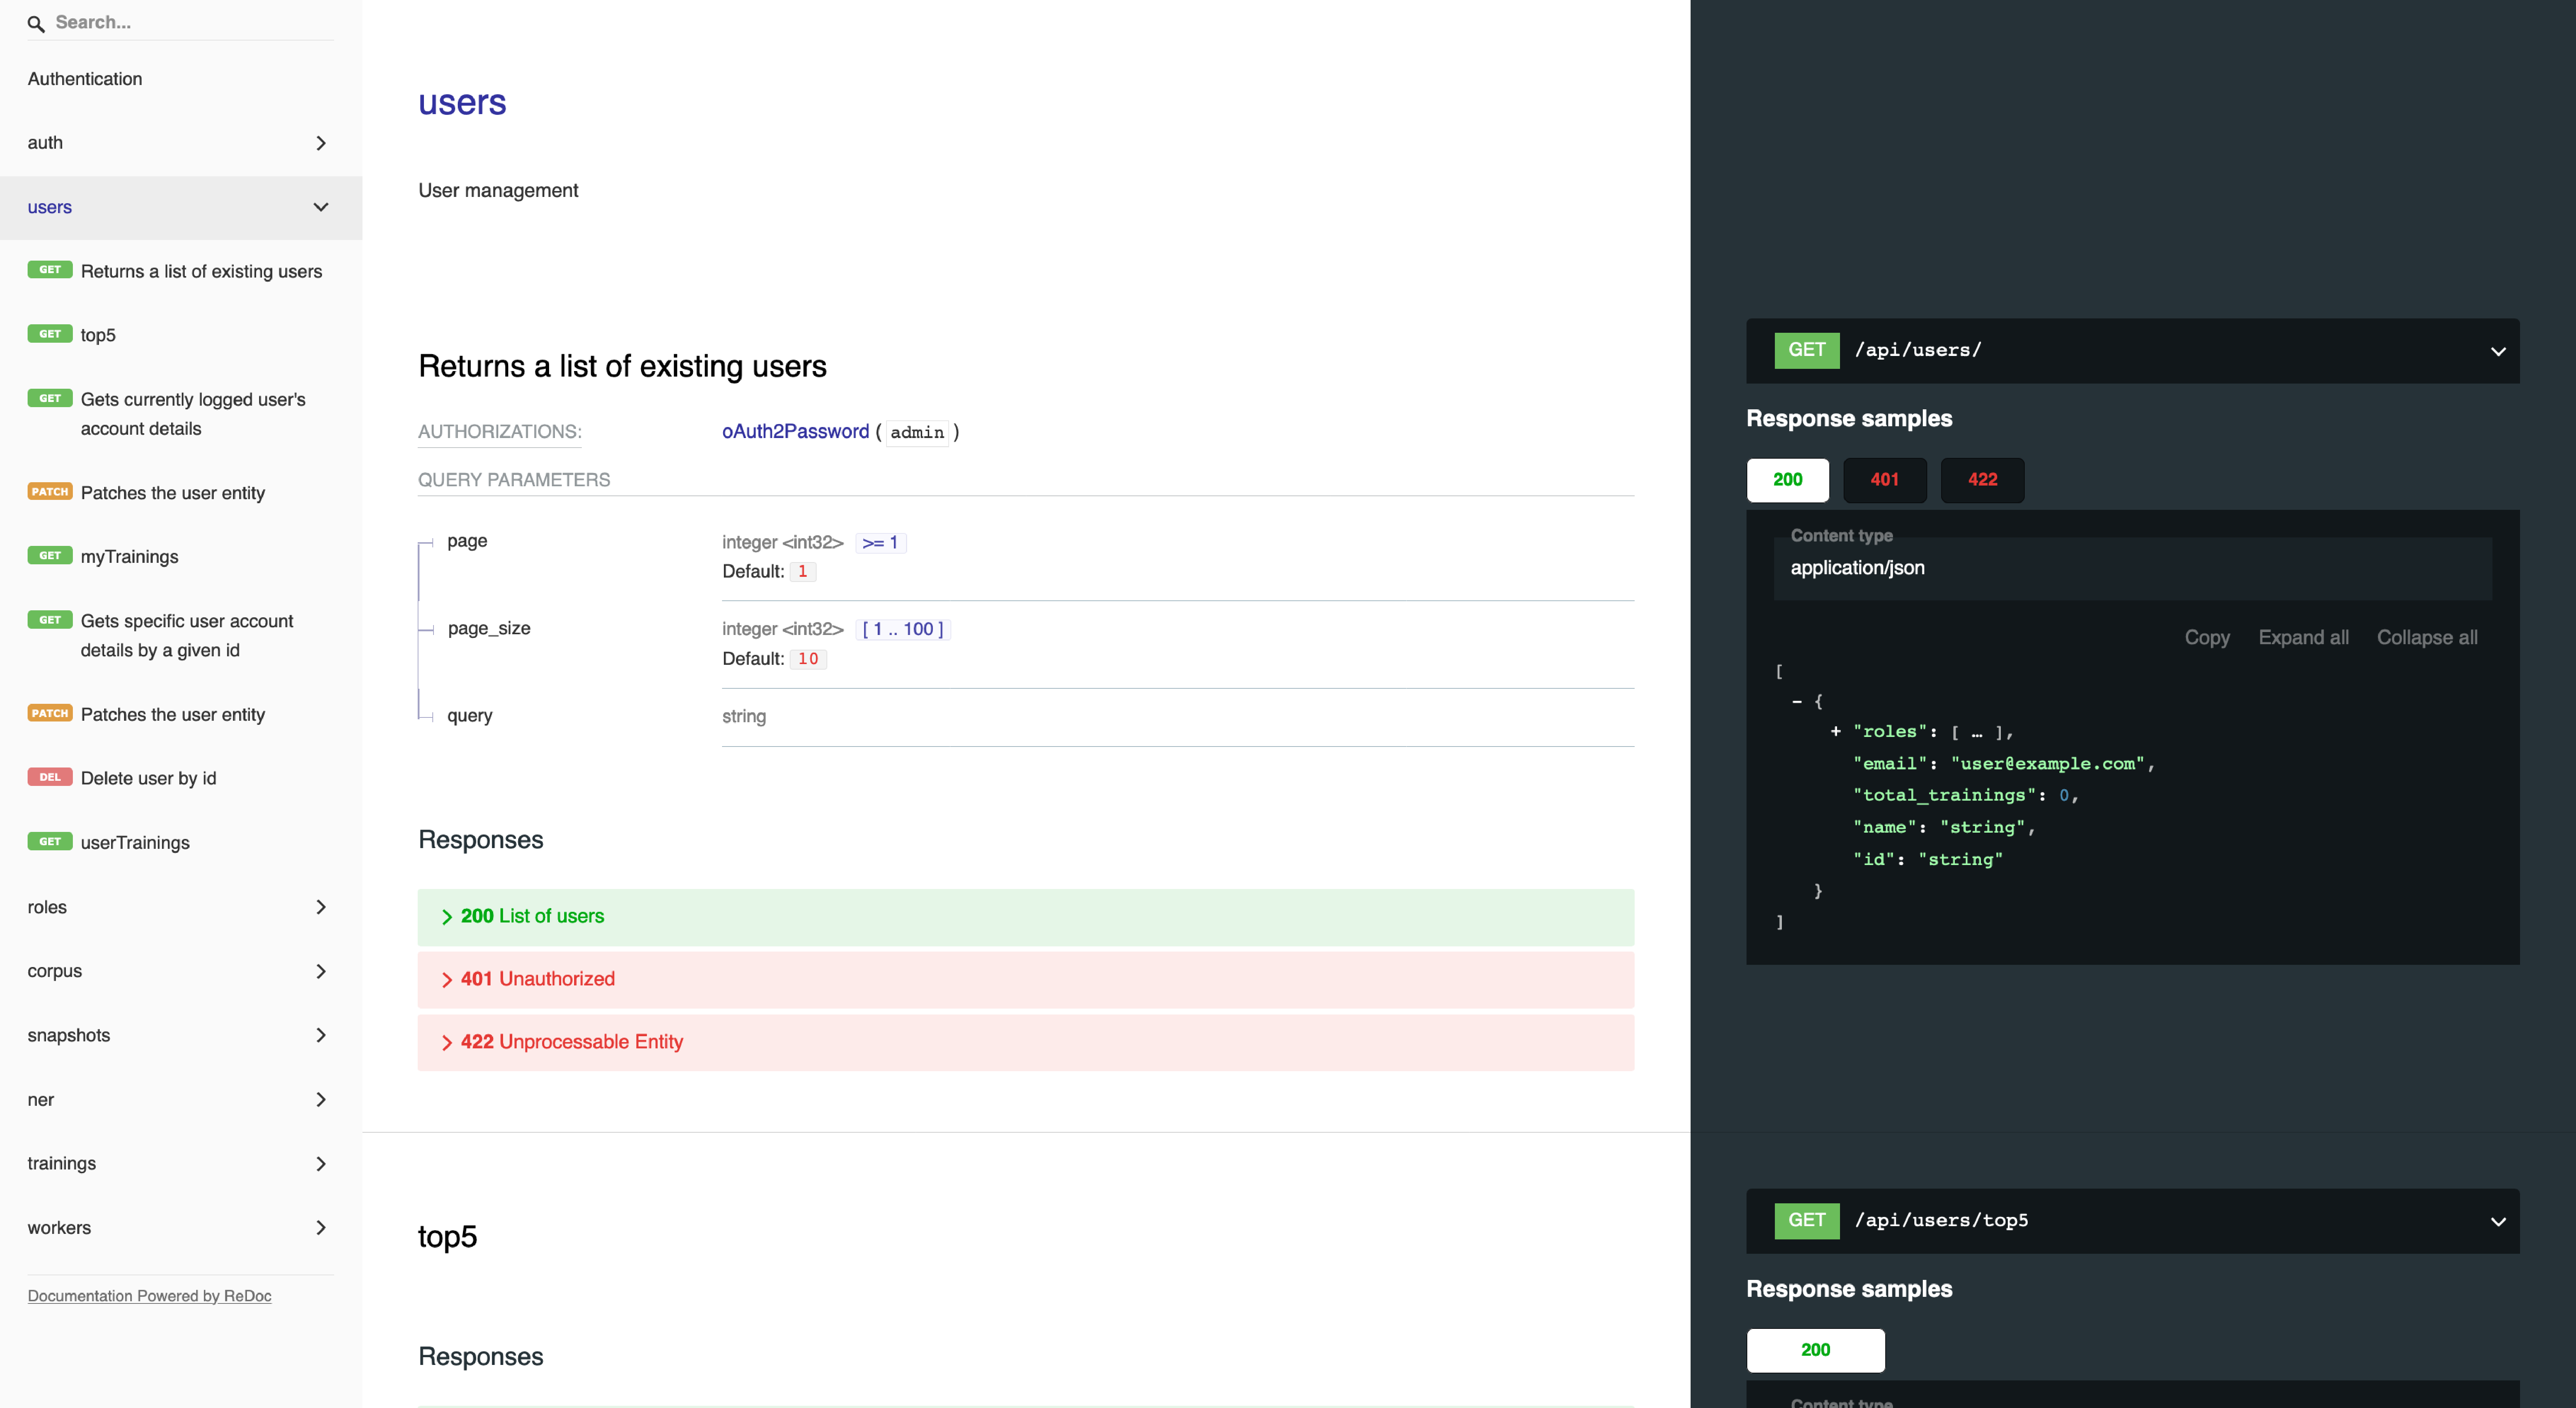
\includegraphics{assets/logic/redoc-main.pdf} 

}

\caption{Ejemplo de documentación con ReDoc.}\label{fig:logic-redoc-main}
\end{figure}

\hypertarget{endpoints}{%
\paragraph{\texorpdfstring{\emph{Endpoints}}{Endpoints}}\label{endpoints}}

\hypertarget{autenticaciuxf3n}{%
\subparagraph{Autenticación}\label{autenticaciuxf3n}}

Rutas del API dedicadas a la autenticación de usuarios.

\begin{itemize}
\tightlist
\item
  \textbf{POST} \texttt{/api/auth/register}

  \begin{itemize}
  \tightlist
  \item
    Registrar un usuario nuevo.
  \end{itemize}
\item
  \textbf{POST} \texttt{/api/auth/token}

  \begin{itemize}
  \tightlist
  \item
    Genera un nuevo \emph{token} de acceso y refresco con credenciales.
  \item
    Utilizado para la funcionalidad de \emph{login}.
  \end{itemize}
\item
  \textbf{POST} \texttt{/api/auth/refresh}

  \begin{itemize}
  \tightlist
  \item
    Refresca el \emph{token} de acceso.
  \item
    Utilizado cuando un \emph{token} de acceso caducó.
  \end{itemize}
\end{itemize}

\hypertarget{usuarios}{%
\subparagraph{Usuarios}\label{usuarios}}

Conjunto de operaciones relacionadas con los usuarios del sistema.

\begin{itemize}
\tightlist
\item
  \textbf{GET} \texttt{/api/users}

  \begin{itemize}
  \tightlist
  \item
    Lista de usuarios existentes.
  \item
    Separa los resultados en páginas.
  \end{itemize}
\item
  \textbf{GET} \texttt{/api/users/top5}

  \begin{itemize}
  \tightlist
  \item
    Lista de los 5 usuarios con más entrenamientos.
  \end{itemize}
\item
  \textbf{GET} \texttt{/api/users/me}

  \begin{itemize}
  \tightlist
  \item
    Retorna la información del usuario logueado.
  \end{itemize}
\item
  \textbf{PATCH} \texttt{/api/users/me}

  \begin{itemize}
  \tightlist
  \item
    Actualiza la información del usuario logueado.
  \end{itemize}
\item
  \textbf{GET} \texttt{/api/users/me/trainings}

  \begin{itemize}
  \tightlist
  \item
    Retorna los entrenamientos del usuario logueado.
  \item
    Separa los resultados en páginas.
  \end{itemize}
\item
  \textbf{GET} \texttt{/api/users/\{user\_id\}}

  \begin{itemize}
  \tightlist
  \item
    Retorna la información del usuario especificado por \texttt{user\_id}.
  \end{itemize}
\item
  \textbf{PATCH} \texttt{/api/users/\{user\_id\}}

  \begin{itemize}
  \tightlist
  \item
    Actualiza la información del usuario especificado por \texttt{user\_id}.
  \end{itemize}
\item
  \textbf{DELETE} \texttt{/api/users/\{user\_id\}}

  \begin{itemize}
  \tightlist
  \item
    Borra al usuario especificado por \texttt{user\_id}.
  \end{itemize}
\item
  \textbf{GET} \texttt{/api/users/\{user\_id\}/trainings}

  \begin{itemize}
  \tightlist
  \item
    Retorna los entrenamientos del usuario especificado.
  \end{itemize}
\end{itemize}

\hypertarget{roles}{%
\subparagraph{Roles}\label{roles}}

\begin{itemize}
\tightlist
\item
  \textbf{GET} \texttt{/api/roles}

  \begin{itemize}
  \tightlist
  \item
    Retorna la lista de todos los roles asignables a usuarios del sistema.
  \end{itemize}
\end{itemize}

\hypertarget{corpus-2}{%
\subparagraph{Corpus}\label{corpus-2}}

Rutas dedicadas a operaciones con el \emph{corpus} del sistema.

\begin{itemize}
\tightlist
\item
  \textbf{GET} \texttt{/api/corpus/\{text\_id\}}

  \begin{itemize}
  \tightlist
  \item
    Retorna los detalles del texto especificado por \texttt{text\_id}.
  \end{itemize}
\item
  \textbf{DELETE} \texttt{/api/corpus/\{text\_id\}}

  \begin{itemize}
  \tightlist
  \item
    Borra un texto especificado por \texttt{text\_id} del corpus.
  \end{itemize}
\item
  \textbf{GET} \texttt{/api/corpus/\{text\_id\}/trainings}

  \begin{itemize}
  \tightlist
  \item
    Retorna la lista de entrenamientos proporcionados por los usuarios sobre las entidades en el texto.
  \end{itemize}
\item
  \textbf{PUT} \texttt{/api/corpus/\{text\_id\}/trainings}

  \begin{itemize}
  \tightlist
  \item
    Agrega un entrenamiento para el texto con id \emph{text\_id}.
  \end{itemize}
\item
  \textbf{POST} \texttt{/api/corpus/upload}

  \begin{itemize}
  \tightlist
  \item
    Permite agregar textos de manera masiva al sistema.
  \item
    Acepta una lista de archivos \texttt{.txt} donde cada línea es un texto a agregar.
  \item
    Los archivos deben ser \texttt{UTF-8}.
  \end{itemize}
\item
  \textbf{GET} \texttt{/api/corpus}

  \begin{itemize}
  \tightlist
  \item
    Lista de textos cargados en el sistema para entrenamiento.
  \item
    Separa los resultados en páginas.
  \end{itemize}
\item
  \textbf{POST} \texttt{/api/corpus}

  \begin{itemize}
  \tightlist
  \item
    Agrega un texto al sistema para entrenamiento.
  \end{itemize}
\end{itemize}

\hypertarget{snapshots-1}{%
\subparagraph{Snapshots}\label{snapshots-1}}

Conjunto de operaciones relacionadas con los snapshots y workers.

\begin{itemize}
\tightlist
\item
  \textbf{GET} \texttt{/api/snapshots}

  \begin{itemize}
  \tightlist
  \item
    Listado de los snapshots disponibles.
  \item
    Separa los resultados en páginas.
  \end{itemize}
\item
  \textbf{GET} \texttt{/api/snapshots/\{snapshot\_id\}}

  \begin{itemize}
  \tightlist
  \item
    Retorna información (tipos de entidades, fecha de creación, fecha de entrenamiento, etc.) sobre un \emph{snapshot} específico.
  \end{itemize}
\item
  \textbf{DELETE} \texttt{/api/snapshots/\{snapshot\_id\}}

  \begin{itemize}
  \tightlist
  \item
    Borra un \emph{snapshot} con el id especificado.
  \end{itemize}
\item
  \textbf{POST} \texttt{/api/snapshots/\{snapshot\_id\}/force-train}

  \begin{itemize}
  \tightlist
  \item
    Envía la tarea de entrenamiento a los workers que tienen el \emph{snapshot} \texttt{snapshot\_id} cargado.
  \end{itemize}
\item
  \textbf{POST} \texttt{/api/snapshots/\{snapshot\_id\}/force-untrain}

  \begin{itemize}
  \tightlist
  \item
    Envía la tarea de desentrenar a los \emph{workers} que tienen el \emph{snapshot}. \emph{snapshot\_id} cargado.
  \end{itemize}
\item
  \textbf{GET} \texttt{/api/snapshots/current}

  \begin{itemize}
  \tightlist
  \item
    Retorna información sobre el \emph{snapshot} actual.
  \end{itemize}
\item
  \textbf{PUT} \texttt{/api/snapshots/current}

  \begin{itemize}
  \tightlist
  \item
    Crea un nuevo \emph{snapshot} con la información provista.
  \end{itemize}
\end{itemize}

\hypertarget{reconocimiento-de-entidades-nombradas}{%
\subparagraph{Reconocimiento de Entidades Nombradas}\label{reconocimiento-de-entidades-nombradas}}

Conjunto de operaciones relacionadas al \emph{Reconocimiento de Entidades Nombradas}

\begin{itemize}
\tightlist
\item
  \textbf{GET} \texttt{/api/ner/train}

  \begin{itemize}
  \tightlist
  \item
    Retorna un texto para que un usuario del sistema revise si está correctamente inferido.
  \item
    Únicamente retorna textos que el usuario logueado no haya corregido ya
  \end{itemize}
\item
  \textbf{GET} \texttt{/api/ner/compare/\{first\_snapshot\}/\{second\_snapshot\}}

  \begin{itemize}
  \tightlist
  \item
    Compara el \emph{NER} entre dos \emph{snapshots} distintos.
  \end{itemize}
\item
  \textbf{POST} \texttt{/api/ner/current/parse}

  \begin{itemize}
  \tightlist
  \item
    Retorna un documento \emph{spaCy} para un texto dado utilizando el \emph{snapshot} actual.
  \end{itemize}
\item
  \textbf{POST} \texttt{/api/ner/\{snapshot\_id\}/parse}

  \begin{itemize}
  \tightlist
  \item
    Retorna un documento \emph{spaCy} para un texto dado utilizando el \emph{snapshot} especificado.
  \end{itemize}
\item
  \textbf{POST} \texttt{/api/ner/current/entities}

  \begin{itemize}
  \tightlist
  \item
    Retorna la lista de \emph{Entidades Nombradas} para un texto dado utilizando el modelo actual.
  \end{itemize}
\item
  \textbf{POST} \texttt{/api/ner/\{snapshot\_id\}/entities}

  \begin{itemize}
  \tightlist
  \item
    Retorna la lista de \emph{Entidades Nombradas} para un texto dado utilizando el modelo especificado.
  \end{itemize}
\end{itemize}

\hypertarget{entrenamientos}{%
\subparagraph{Entrenamientos}\label{entrenamientos}}

\begin{itemize}
\tightlist
\item
  \textbf{DELETE} \texttt{/api/trainings/\{training\_id\}}

  \begin{itemize}
  \tightlist
  \item
    Borra un entrenamiento.
  \end{itemize}
\end{itemize}

\hypertarget{workers}{%
\subparagraph{Workers}\label{workers}}

\begin{itemize}
\tightlist
\item
  \textbf{GET} \texttt{/api/workers/}

  \begin{itemize}
  \tightlist
  \item
    Lista de los workers disponibles.
  \end{itemize}
\item
  \textbf{POST} \texttt{/api/workers/reassign}

  \begin{itemize}
  \tightlist
  \item
    Reasigna un trabajador de un a versión de \emph{snapshot} a otra.
  \end{itemize}
\end{itemize}

\hypertarget{vista-de-proceso}{%
\subsection{Vista de proceso}\label{vista-de-proceso}}

\begin{quote}
La vista de proceso trata los aspectos dinámicos del sistema, explica los procesos del sistema y cómo se comunican, y se centra en el comportamiento del sistema en tiempo de ejecución.
La vista de proceso aborda concurrencia, distribución, integradores, rendimiento y escalabilidad, etc.
\end{quote}

Como podemos ver en la figura \ref{fig:process-overview-client}, existen cinco procesos que juntos forman la totalidad de NERd y su entrenador.

\begin{figure}[H]

{\centering 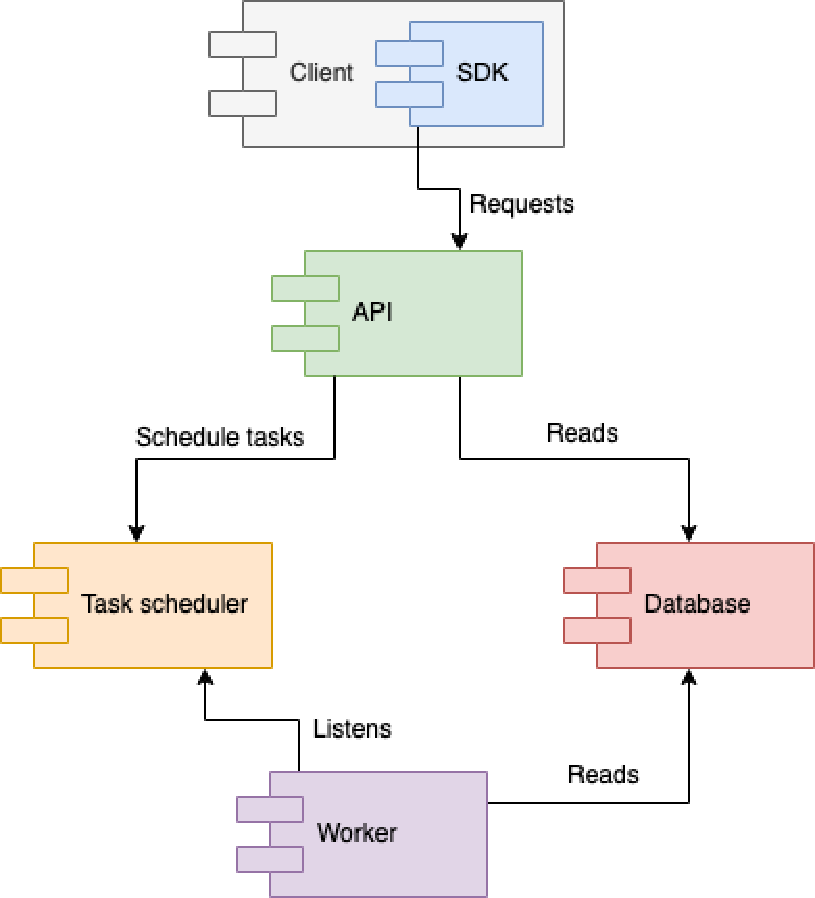
\includegraphics{assets/process/process-overview-client.pdf} 

}

\caption{Componentes del sistema.}\label{fig:process-overview-client}
\end{figure}

\hypertarget{api-1}{%
\subsubsection{API}\label{api-1}}

Servicio en el cual los clientes pueden pedir las \emph{Entidades Nombradas} de textos así como también permite la carga de textos con sus respectivas correcciones que luego serán utilizadas para entrenar el modelo de inferencia.
El \emph{API} se comunica el servicio de \emph{Bases de Datos} para obtener o modificar información sobre los usuarios, los textos pertenecientes al \emph{corpus} o información de los distintos \emph{snapshots} y envía mensajes al \emph{Task Scheduler} para realizar diversas tareas relacionadas con \emph{spaCy} así como también tareas de administración sobre los \emph{workers} disponibles.

\hypertarget{task-scheduler}{%
\subsubsection{Task Scheduler}\label{task-scheduler}}

Recibe tareas desde el \emph{API} tales como reconocer entidades, entrenar y desentrenar un modelo, cambiar el modelo de un worker entre otras. A el task scheduler se suscriben todos los \emph{workers} del sistema de manera tal de poder recibir mensajes y realizar acciones.
Su funcionamiento es crítico para poder manejar grandes volúmenes de consultas al motor de inferencia ya que permite generar una estructura que escale horizontalmente debido a la posibilidad de contar con la suscripción de un número arbitrario de \emph{workers}.

\hypertarget{worker}{%
\subsubsection{Worker}\label{worker}}

Un \emph{Worker} se encarga de realizar el \emph{Reconocimiento de Entidades Nombradas} así como también de entrenar modelos de inferencia. Es un servicio que existe de manera independiente y necesita de dos otros servicios para funcionar:

\begin{itemize}
\tightlist
\item
  \emph{Base de datos} para obtener los datos necesarios para entrenar un modelo.
\item
  \emph{Task scheduler} para poder recibir tareas.
\end{itemize}

Como el \emph{Worker} es una unidad de trabajo que recibe tareas desde el \emph{Task Scheduler}, es posible tener varios \emph{Workers} donde cada uno utiliza un modelo de inferencia distinto (generados a partir de distintos snapshots).

Cuando un \emph{Worker} es creado, automáticamente carga el modelo actual (\emph{current snapshot}) y se suscribe a la cola de mensajes para esa versión en particular.

\hypertarget{database}{%
\subsubsection{Database}\label{database}}

Servicio que contiene la base de datos con la información necesaria (usuarios, snapshots) para que el servicio de \emph{API} funcione así como también los datos necesarios por los workers (entrenamientos).

\hypertarget{cliente}{%
\subsubsection{Cliente}\label{cliente}}

Es la interfaz del entrenador que se comunica con el API utilizando un \emph{SDK} auto-generado a partir de la definición de \emph{OpenAPI}. Implementado en este proyecto es un cliente \emph{web} el cual permite explotar las funcionalidades de entrenamiento así como de inferencia de entidades.

\hypertarget{vista-de-desarrollo}{%
\subsection{Vista de desarrollo}\label{vista-de-desarrollo}}

\begin{quote}
La vista de desarrollo ilustra un sistema desde la perspectiva de un programador y se ocupa de la gestión de software.
Esta vista también se conoce como la vista de implementación.
\end{quote}

\hypertarget{web-1}{%
\subsubsection{Web}\label{web-1}}

La página \emph{web} que contiene la interfaz de administración así como también la de entrenamiento. Para implementarla decidimos utilizar el modelo de \emph{Single Page Application} que nos permitió generar un \emph{bundle} que puede ser hosteado en \emph{CDNs} y nos permite tener ciclos de release independientes al los del servicio.

Poder separar las releases de la \emph{web} y el servicio es importante ya que los clientes del servicio no necesariamente necesitan de la web, ya que pueden acceder al servicio mediante el \emph{API REST} y una baja por cambios a la interfaz de la \emph{web} no afecta la disponibilidad del servicio.

\hypertarget{tecnologuxedas}{%
\paragraph{Tecnologías}\label{tecnologuxedas}}

Para la implementación utilizamos el lenguaje de programación llamado \textbf{Typescript}, lenguaje desarrollado por \emph{Microsoft} que compila a \emph{JavaScript} con el agregado de \emph{Tipos} que permiten producir código de mayor calidad debido al agregado de la posibilidad del chequeo estático de código para validar su correctitud.

Una vez definido el lenguaje, optamos por utilizar la librería llamada \textbf{ReactJS} (Facebook, \protect\hyperlink{ref-react}{2019}) desarrollada por \emph{Facebook} para implementar la interfaz.

Sumado a \textbf{ReactJS}, incluímos diversas librerías para poder resolver varios problemas en el desarrollo de una \emph{SPA}:

\hypertarget{material-ui}{%
\subparagraph{Material UI}\label{material-ui}}

Provee de una biblioteca de componentes estilados siguiendo el patrón de diseño propuesto por \emph{Google} llamado \emph{Material Design}.

\hypertarget{react-router}{%
\subparagraph{React Router}\label{react-router}}

Desarrollada por \emph{React Training}, proveé de mecanimos para la navegación en \emph{SPAs}.

\hypertarget{i18next}{%
\subparagraph{i18next}\label{i18next}}

Librería que proveé mecanismos de internacionalización. A su vez, nos permitió generar los archivos de traducción mediante su extracción del código fuente utilizando la herramienta \texttt{i18next-scanner}.

\hypertarget{openapi-generator}{%
\subparagraph{OpenAPI Generator}\label{openapi-generator}}

\emph{OpenAPI Generator} es una herramienta que permite generar código a partir de una definición de \emph{OpenAPI}.
Debido a que el servicio implementado expone una definiciión de \emph{OpenAPI}, podemos utilizar ésta librería para auto-generar todo el código necesario para comunicarnos con el servicio usando el generador de \emph{Typescript}.

\hypertarget{arquitectura}{%
\paragraph{Arquitectura}\label{arquitectura}}

El código en la \emph{web} se encuentra separado por rasgos, ya sean de utilidad, como modelos o funciones, o de funcionalidad, como la vista de la pantalla de inicio (Figura \ref{fig:developer-web-modules}).

\begin{figure}[H]

{\centering 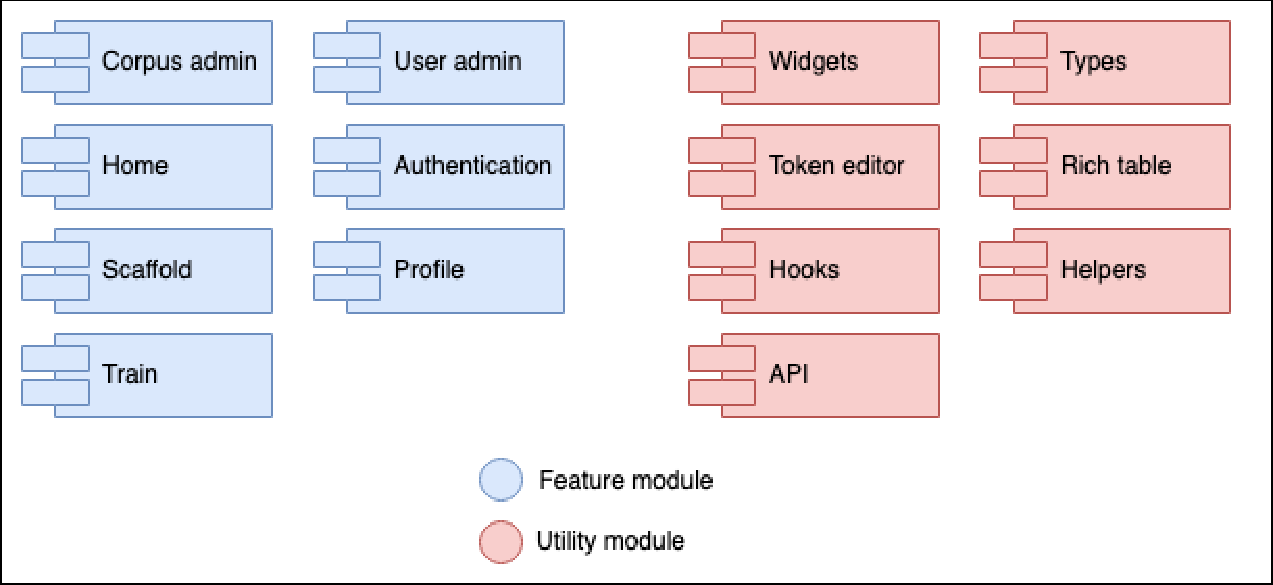
\includegraphics{assets/developer/web-modules.pdf} 

}

\caption{Módulos de la página web.}\label{fig:developer-web-modules}
\end{figure}

Los módulos marcados en azul son relacionados al contenido que se muestra cada ruta del sistema.

Los módulos marcados en rojos son de utilidad, ya sea por que contienen todo el código relevante a la comunicación con el \emph{API REST} o a componentes utilizados en varias áreas de los módulos azules.

\hypertarget{sesiuxf3n}{%
\paragraph{Sesión}\label{sesiuxf3n}}

El servicio \emph{web} ofrece la posibilidad de recordar la sesión de un usuario en el momento de realizar el login. De elegirse, las credenciales son guardadas en el \emph{local storage} del cliente web, de manera tal que el usuario pueda utilizar la misma sesión por más de que haya cerrado el cliente web.

Si en algún momento en el futuro el \emph{API} nos retorna algún request indicando que el usuario no tiene permisos para acceder a algún área (código HTTP 401) y el token de refrescado dejó de ser válido, las credenciales se borran del \emph{local storage} y redirigimos al cliente a la pantalla de inicio.

Ofrecemos también la posibilidad de no guardar la sesión, lo cual hará que una vez cerrada la pestaña, el usuario deba volver a ingresar al sistema para poder acceder a los distintos servicios.

\hypertarget{internacionalizaciuxf3n}{%
\paragraph{Internacionalización}\label{internacionalizaciuxf3n}}

Así como las credenciales, las preferencias de internacionalización son guardadas en el \emph{local storage} del cliente web, de manera tal que los usuarios del sistema no deban elegir el idioma de su preferencia cada vez que ingresan a la página.

\hypertarget{api-2}{%
\subsubsection{\texorpdfstring{\emph{API}}{API}}\label{api-2}}

Implementada utilizando el lenguaje de programación \emph{Python}. El principal motivador de esta elección fue que las librerías que más se acercan al estado del arte en \emph{Machine Learning} se encuentran implementadas en este lenguaje. Provee del servicio al cual acceden los usuarios, tales como la plataforma \emph{web} de entrenamiento mediante la implementación de un \emph{API} \emph{REST}.

\hypertarget{tecnologuxedas-1}{%
\paragraph{Tecnologías}\label{tecnologuxedas-1}}

\hypertarget{flask}{%
\subparagraph{\texorpdfstring{\emph{Flask}}{Flask}}\label{flask}}

Como base del proyecto utilizamos un \emph{microframework} de aplicaciones \emph{web} llamado \emph{Flask} (``Flask,'' \protect\hyperlink{ref-flask}{2019}) ya que por diseño utiliza pocos recursos. Por defecto no incluye ninguna solución para comunicarse con una base de datos, ni lógica para validar formularios.

\hypertarget{flask-smorest}{%
\subparagraph{\texorpdfstring{\emph{flask-smorest}}{flask-smorest}}\label{flask-smorest}}

\emph{Framework} que enriquece a \emph{Flask} agregando la posibilidad de poder crear \emph{APIs REST} que se auto-documentan generando una especificación de \emph{OpenAPI} que es expuesta a los usuarios del servicio en dos variantes: \emph{ReDoc} y \emph{Swagger UI}. Tener un \emph{API} que se auto-documenta nos permite ofrecerle a los clientes un lugar en el cual puedan consultar el funcionamiento completo de el servicio requiriendo poco trabajo extra a la hora de desarrollar el servicio.

A su vez, provee facilidades de serialización y de-serialización de objetos en respuestas \emph{JSON} utilizando la librería de \emph{marshmallow} así como también utilizades para simplificar la creación de \emph{endpoints} que permitan paginar sus resultados (particularmente útil para listar entidades como entrenamientos, usuarios o textos).

\hypertarget{flask-jwt-extended}{%
\subparagraph{\texorpdfstring{\emph{flask-jwt-extended}}{flask-jwt-extended}}\label{flask-jwt-extended}}

\emph{Flask JWT extended} es una librería que agrega a \emph{Flask} la funcionalidad de poder restringir el acceso a ciertos \emph{endpoints} requiriendo que el usuario tenga un \emph{JSON Web Token} (Jones, Bradley, Sakimura, NRI, \& Microsoft, \protect\hyperlink{ref-JWT}{2015}) que acredite su identidad. A su vez, dado que cada \emph{token} se asocia a una identidad (usuario) y es capaz de contener información, podemos utilizar el mismo sistema para guardar los roles del usuario y requerir que cuente con los permisos necesarios.

\hypertarget{mongoengine}{%
\subparagraph{\texorpdfstring{\emph{Mongoengine}}{Mongoengine}}\label{mongoengine}}

\emph{Mongoengine} es una librería pensada para trabajar con \emph{MongoDB} en \emph{Python}. En su esencia es un \emph{Document-Object Mapper} que permite convertir resultados de consultas de la base de datos en objetos de \emph{Python} así como también permite guardar esos objetos en la base de datos.

\hypertarget{marshmallow-mongoengine}{%
\subparagraph{\texorpdfstring{\emph{marshmallow-mongoengine}}{marshmallow-mongoengine}}\label{marshmallow-mongoengine}}

Librería que nos permite integrar la librería de serialización \emph{Marshmallow} con \emph{Mongoengine} simplificando el manejo de objetos entre la base de datos y los objetos que se serializan o deserializan en la capa del \emph{API}. Es de especial utilidad la posibilidad de excluir campos a serializar ya que permite retornar únicamente lo que es de interés para el usuario, como por ejemplo sucede al retornar un objeto \emph{User} ya nunca deberíamos devolver en una respuesta el campo \emph{password} de la base de datos.

\hypertarget{MongoDBDev}{%
\subsubsection{Base de Datos}\label{MongoDBDev}}

Debido a que en el proyecto necesitamos guardar mayormente documentos (entrenamientos), optamos por utilizar una base de datos orientada a documentos: \emph{MongoDB} (``MongoDB,'' \protect\hyperlink{ref-mongodb}{2019}).

\emph{MongoDB} nos permite tener un lugar en donde guardar todos los documentos que puede escalar tanto como sea necesario debido a su posibilidad de fragmentar\footnote{\url{https://docs.mongodb.com/manual/sharding/}} o replicar\footnote{\url{https://docs.mongodb.com/manual/replication/}} información entre distintas instancias que pueden estar ubicadas en distintos servidores.

\hypertarget{modelado}{%
\paragraph{Modelado}\label{modelado}}

Para el modelado de los datos utilizamos cuatro colecciones mostradas en la figura \ref{fig:developer-db-overview}.

\begin{figure}[H]

{\centering 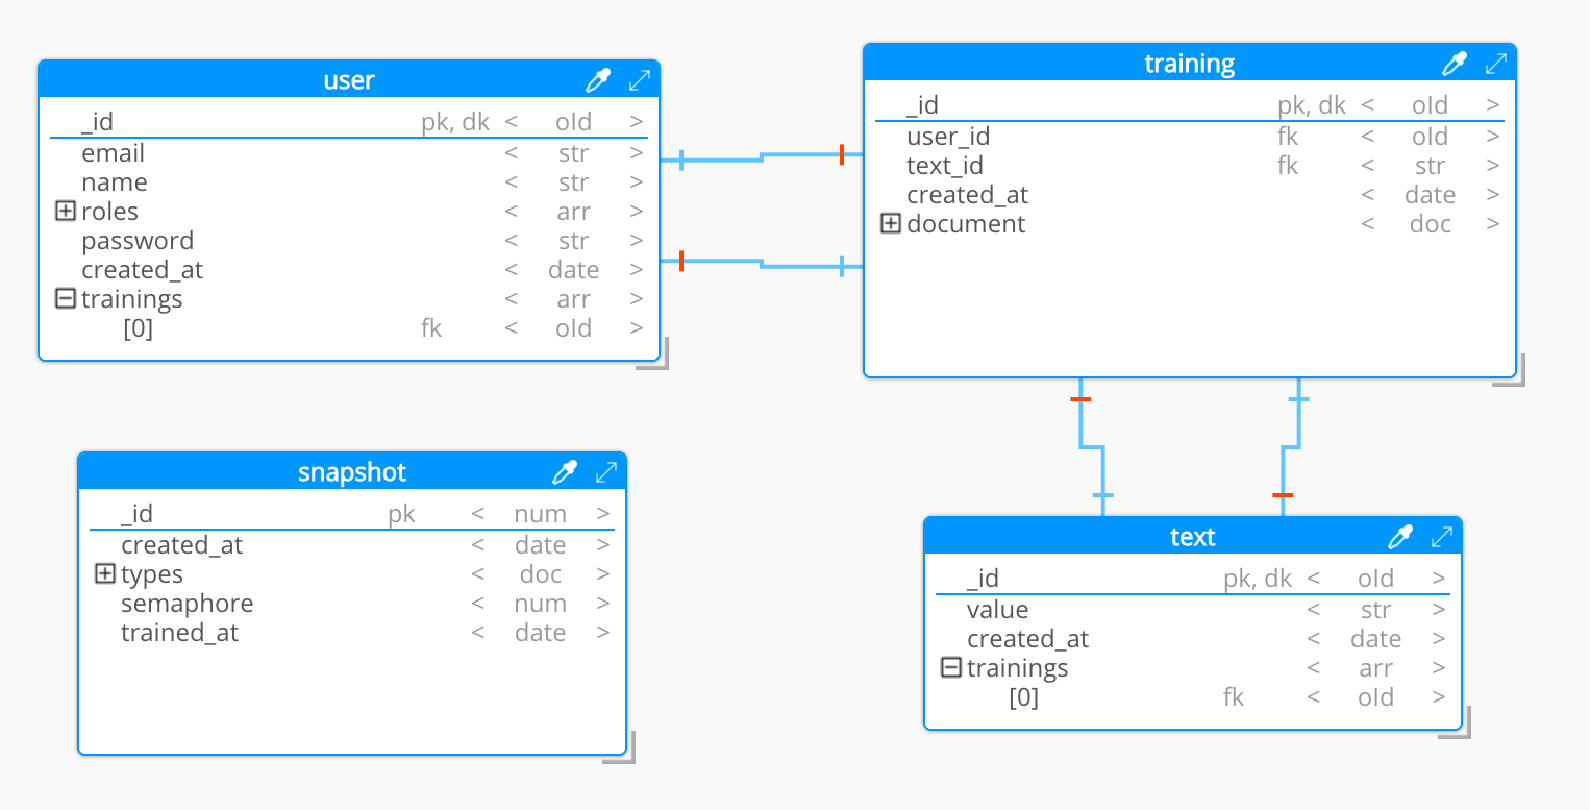
\includegraphics{assets/developer/db-overview.pdf} 

}

\caption{Colecciones de la base de datos.}\label{fig:developer-db-overview}
\end{figure}

\hypertarget{user}{%
\subparagraph{\texorpdfstring{\emph{User}}{User}}\label{user}}

La colección \emph{user} contiene la información de todos los usuarios del sistema (Figura \ref{fig:developer-db-user}). Entre los datos del usuario está el campo \emph{trainings}, que guarda internamente una lista de \emph{ObjectId} pertenecientes a los entrenamientos del usuario. A su vez está la lista de roles a los cuales tiene acceso el usuario.

\begin{figure}[H]

{\centering 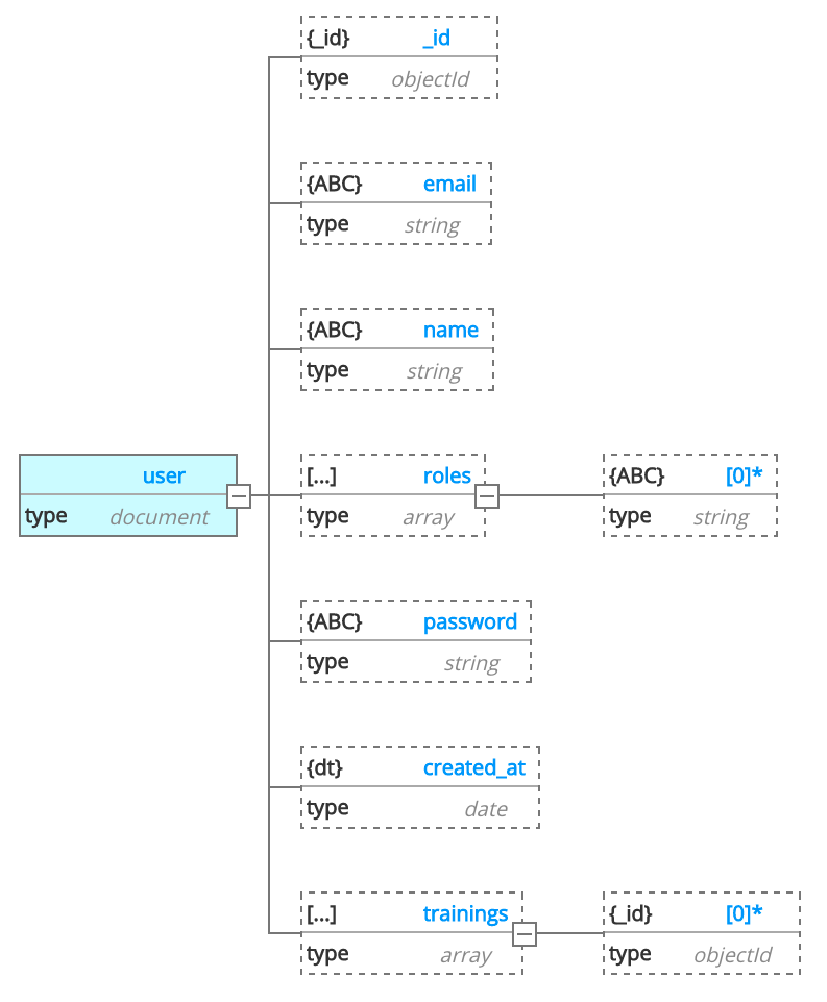
\includegraphics{assets/developer/db-user.pdf} 

}

\caption{Colección de usuarios.}\label{fig:developer-db-user}
\end{figure}

\hypertarget{text}{%
\subparagraph{\texorpdfstring{\emph{Text}}{Text}}\label{text}}

La colección \emph{text} contiene todos los textos que forman parte del corpus que son cargados para ser mostrados en la interfaz de entrenamiento (Figura \ref{fig:developer-db-text}). Así como \emph{user}, cada documento de \emph{text} contiene una lista de referencias a los entrenamientos para ese texto.

\begin{figure}[H]

{\centering 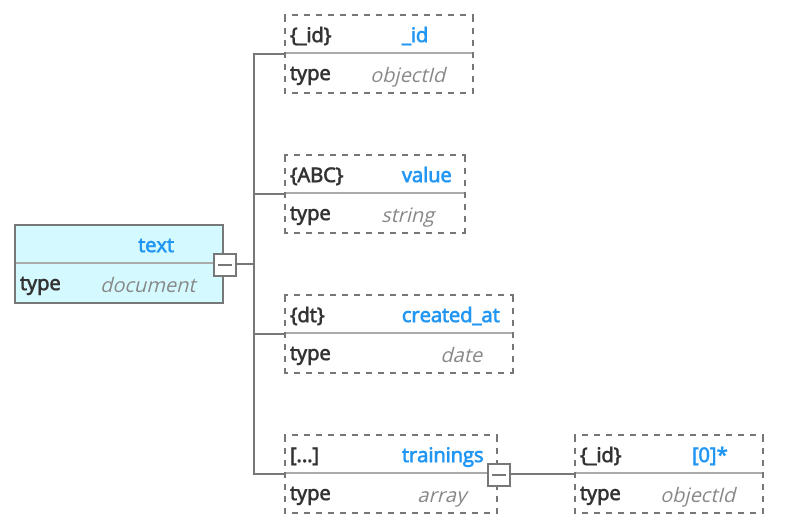
\includegraphics{assets/developer/db-text.png} 

}

\caption{Colección de textos.}\label{fig:developer-db-text}
\end{figure}

\hypertarget{snapshot}{%
\subparagraph{\texorpdfstring{\emph{Snapshot}}{Snapshot}}\label{snapshot}}

La colección \emph{snapshot} contiene información sobre los distintos \emph{snapshots} creados en el sistema (Figura \ref{fig:developer-db-snapshot}). De particular interés es el atributo \emph{types}, que contiene un mapa de todos los tipos de entidades disponibles en el snapshot. También contiene el atributo \emph{semaphore}, que sirve como un campo de control para poder organizar a los \emph{workers} que están utilizando ese \emph{snapshot} en particular.

\begin{figure}[H]

{\centering 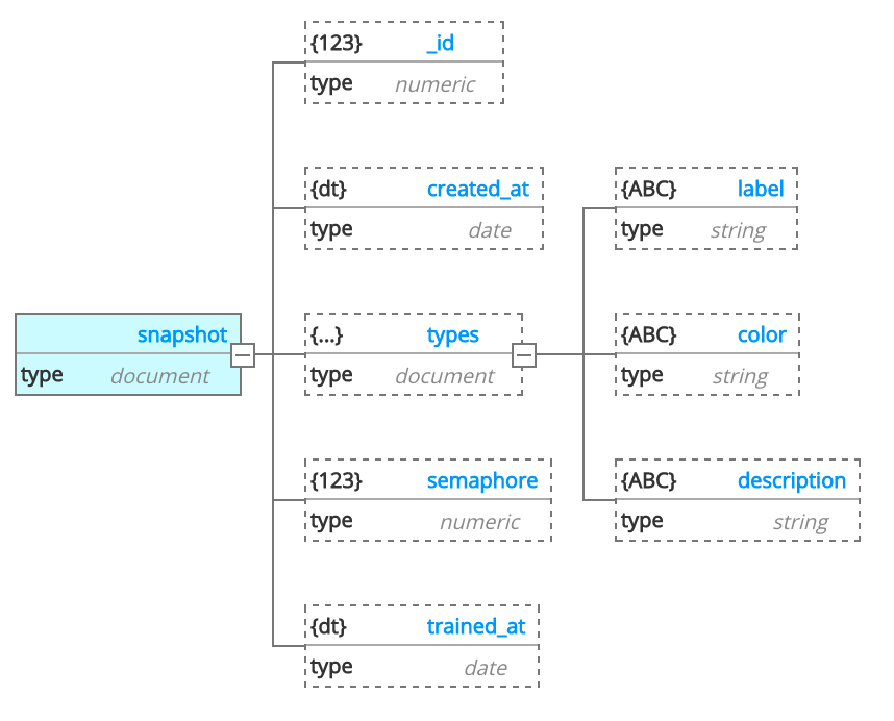
\includegraphics{assets/developer/db-snapshot.pdf} 

}

\caption{Colección de snapshots.}\label{fig:developer-db-snapshot}
\end{figure}

\hypertarget{training}{%
\subparagraph{\texorpdfstring{\emph{Training}}{Training}}\label{training}}

La colección \emph{training} contiene información sobre todos los entrenamientos cargados en el sistema (Figura \ref{fig:developer-db-training}). Cada entrenamiento contiene referencia al texto al que pertenece así como también al usuario que lo creó. De manera tal de poder obtener la información de los documentos relacionados sin necesidad de duplicar información.

Dentro de un documento training, se encuentra el atributo \emph{document}, que es el que internamente contiene la representación de un documento de entrenamiento que es entendido por \emph{spaCy} y que luego será utilizado para entrenar el modelo de inferencia.

\begin{figure}[H]

{\centering 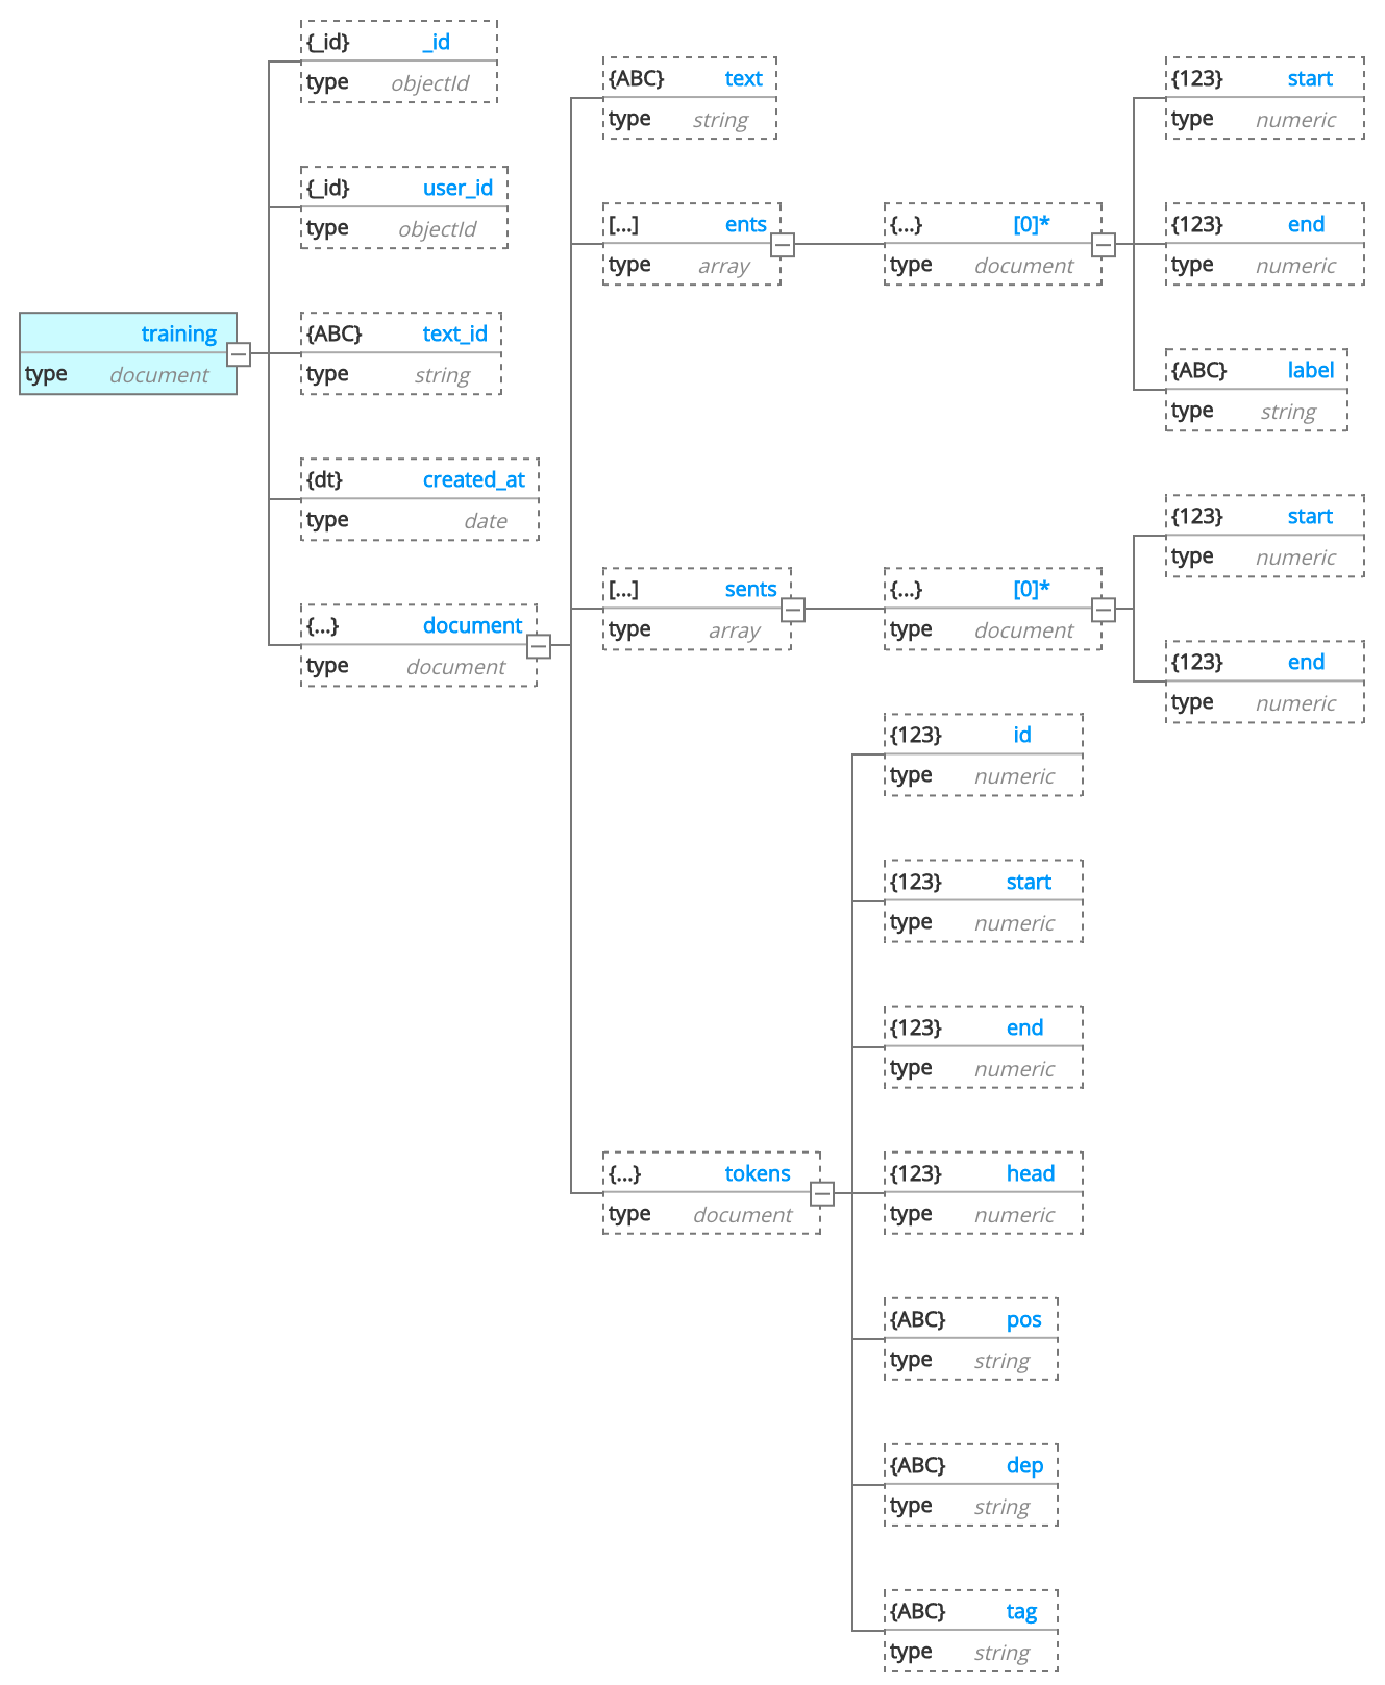
\includegraphics{assets/developer/db-training.pdf} 

}

\caption{Colección de entrenamientos.}\label{fig:developer-db-training}
\end{figure}

\hypertarget{task-scheduler-1}{%
\subsubsection{\texorpdfstring{\emph{Task Scheduler}}{Task Scheduler}}\label{task-scheduler-1}}

El \emph{task scheduler} que utilizamos en el \emph{API} para poder orquestrar todas las tareas relacionadas con \emph{NER} así como también la de la administración de los \emph{workers} es \emph{Celery} (``Celery,'' \protect\hyperlink{ref-celery}{2019}). \emph{Celery} es una cola de tareas asincrónica especializada en el procesamiento distribuido de las mismas. Si bien soporta distintos \emph{backends} para la funcionalidad de cola de mensajes, decidimos utilizar \emph{RabbitMQ} (``RabbitMQ,'' \protect\hyperlink{ref-rabbitmq}{2019}) debido a su buena integración con \emph{Celery} así como también por su robustez y posibilidad de escalar horizontalmente.

Para el monitoreo de las tareas de \emph{Celery} utilizamos la herramienta llamada \emph{Flower} (Movsisyan, \protect\hyperlink{ref-flower}{2016}), que permite cosas como el estado de cada worker (Figura \ref{fig:developer-flower-dashboard}), historial de tareas (Figura \ref{fig:developer-flower-task-history}) así como también estadísticas en tiempo real sobre el sistema (Figura \ref{fig:developer-flower-monitoring}) y detalles de todos los trabajadores que están conectados a la cola de mensajes (Figura \ref{fig:developer-flower-monitoring}).

\begin{figure}[H]

{\centering 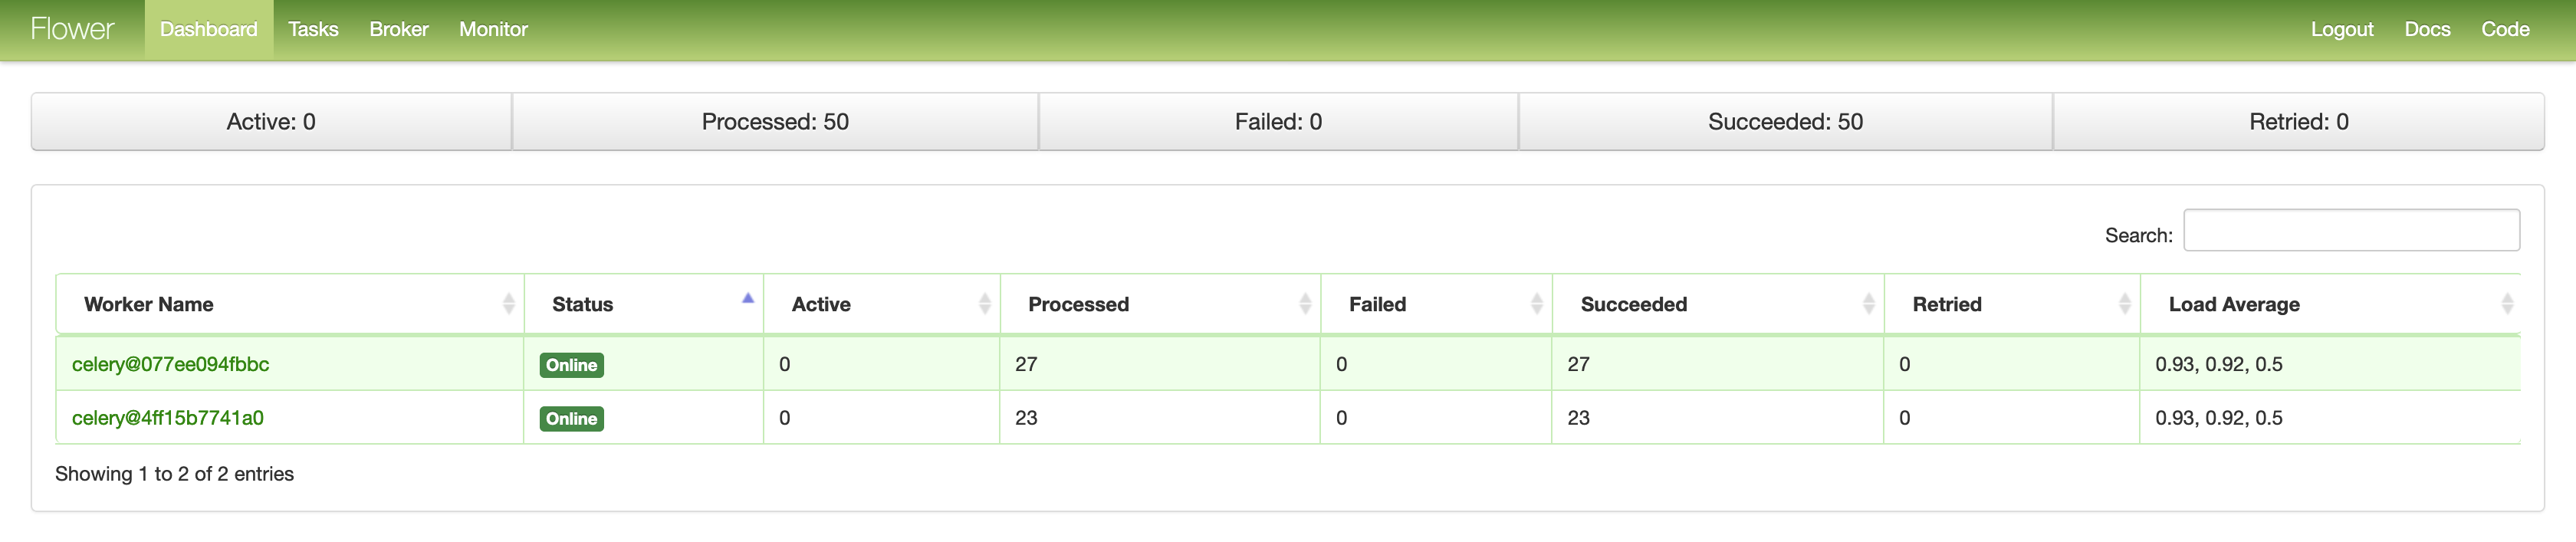
\includegraphics{assets/developer/flower-dashboard.png} 

}

\caption{Página principal de Flower.}\label{fig:developer-flower-dashboard}
\end{figure}

\begin{figure}[H]

{\centering 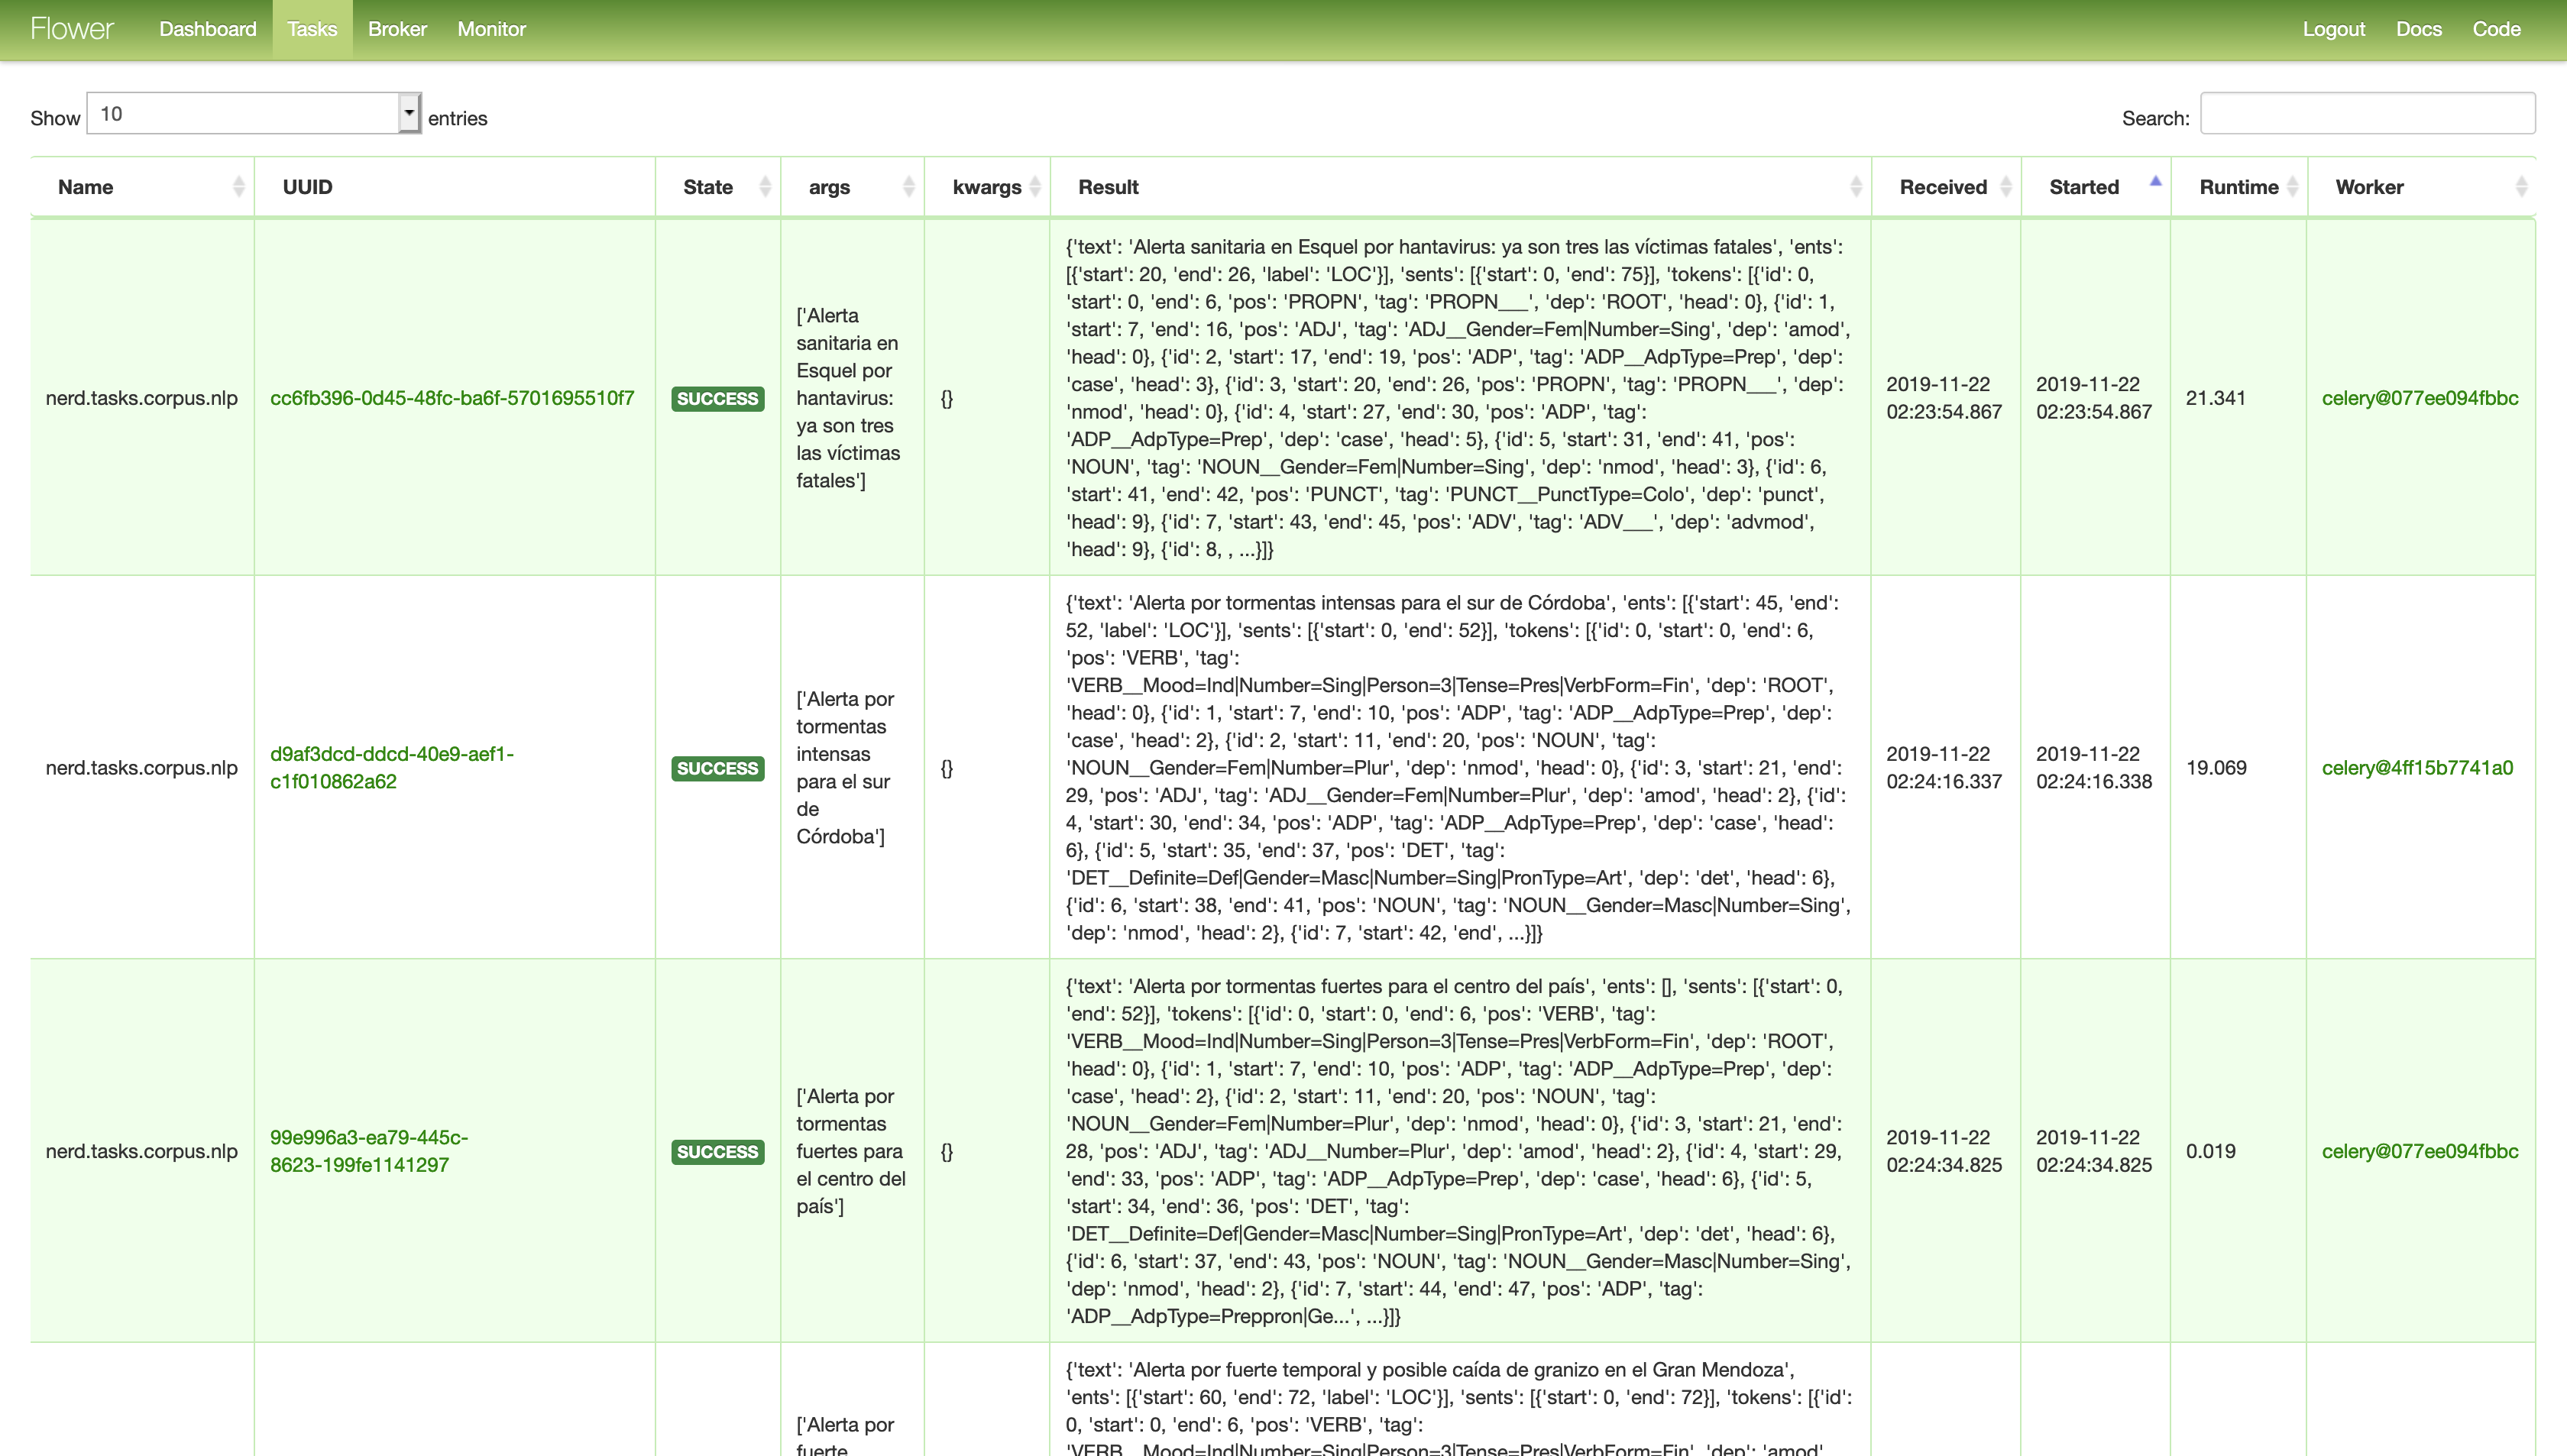
\includegraphics{assets/developer/flower-task-history.png} 

}

\caption{Historial de tareas en Flower.}\label{fig:developer-flower-task-history}
\end{figure}

\begin{figure}[H]

{\centering 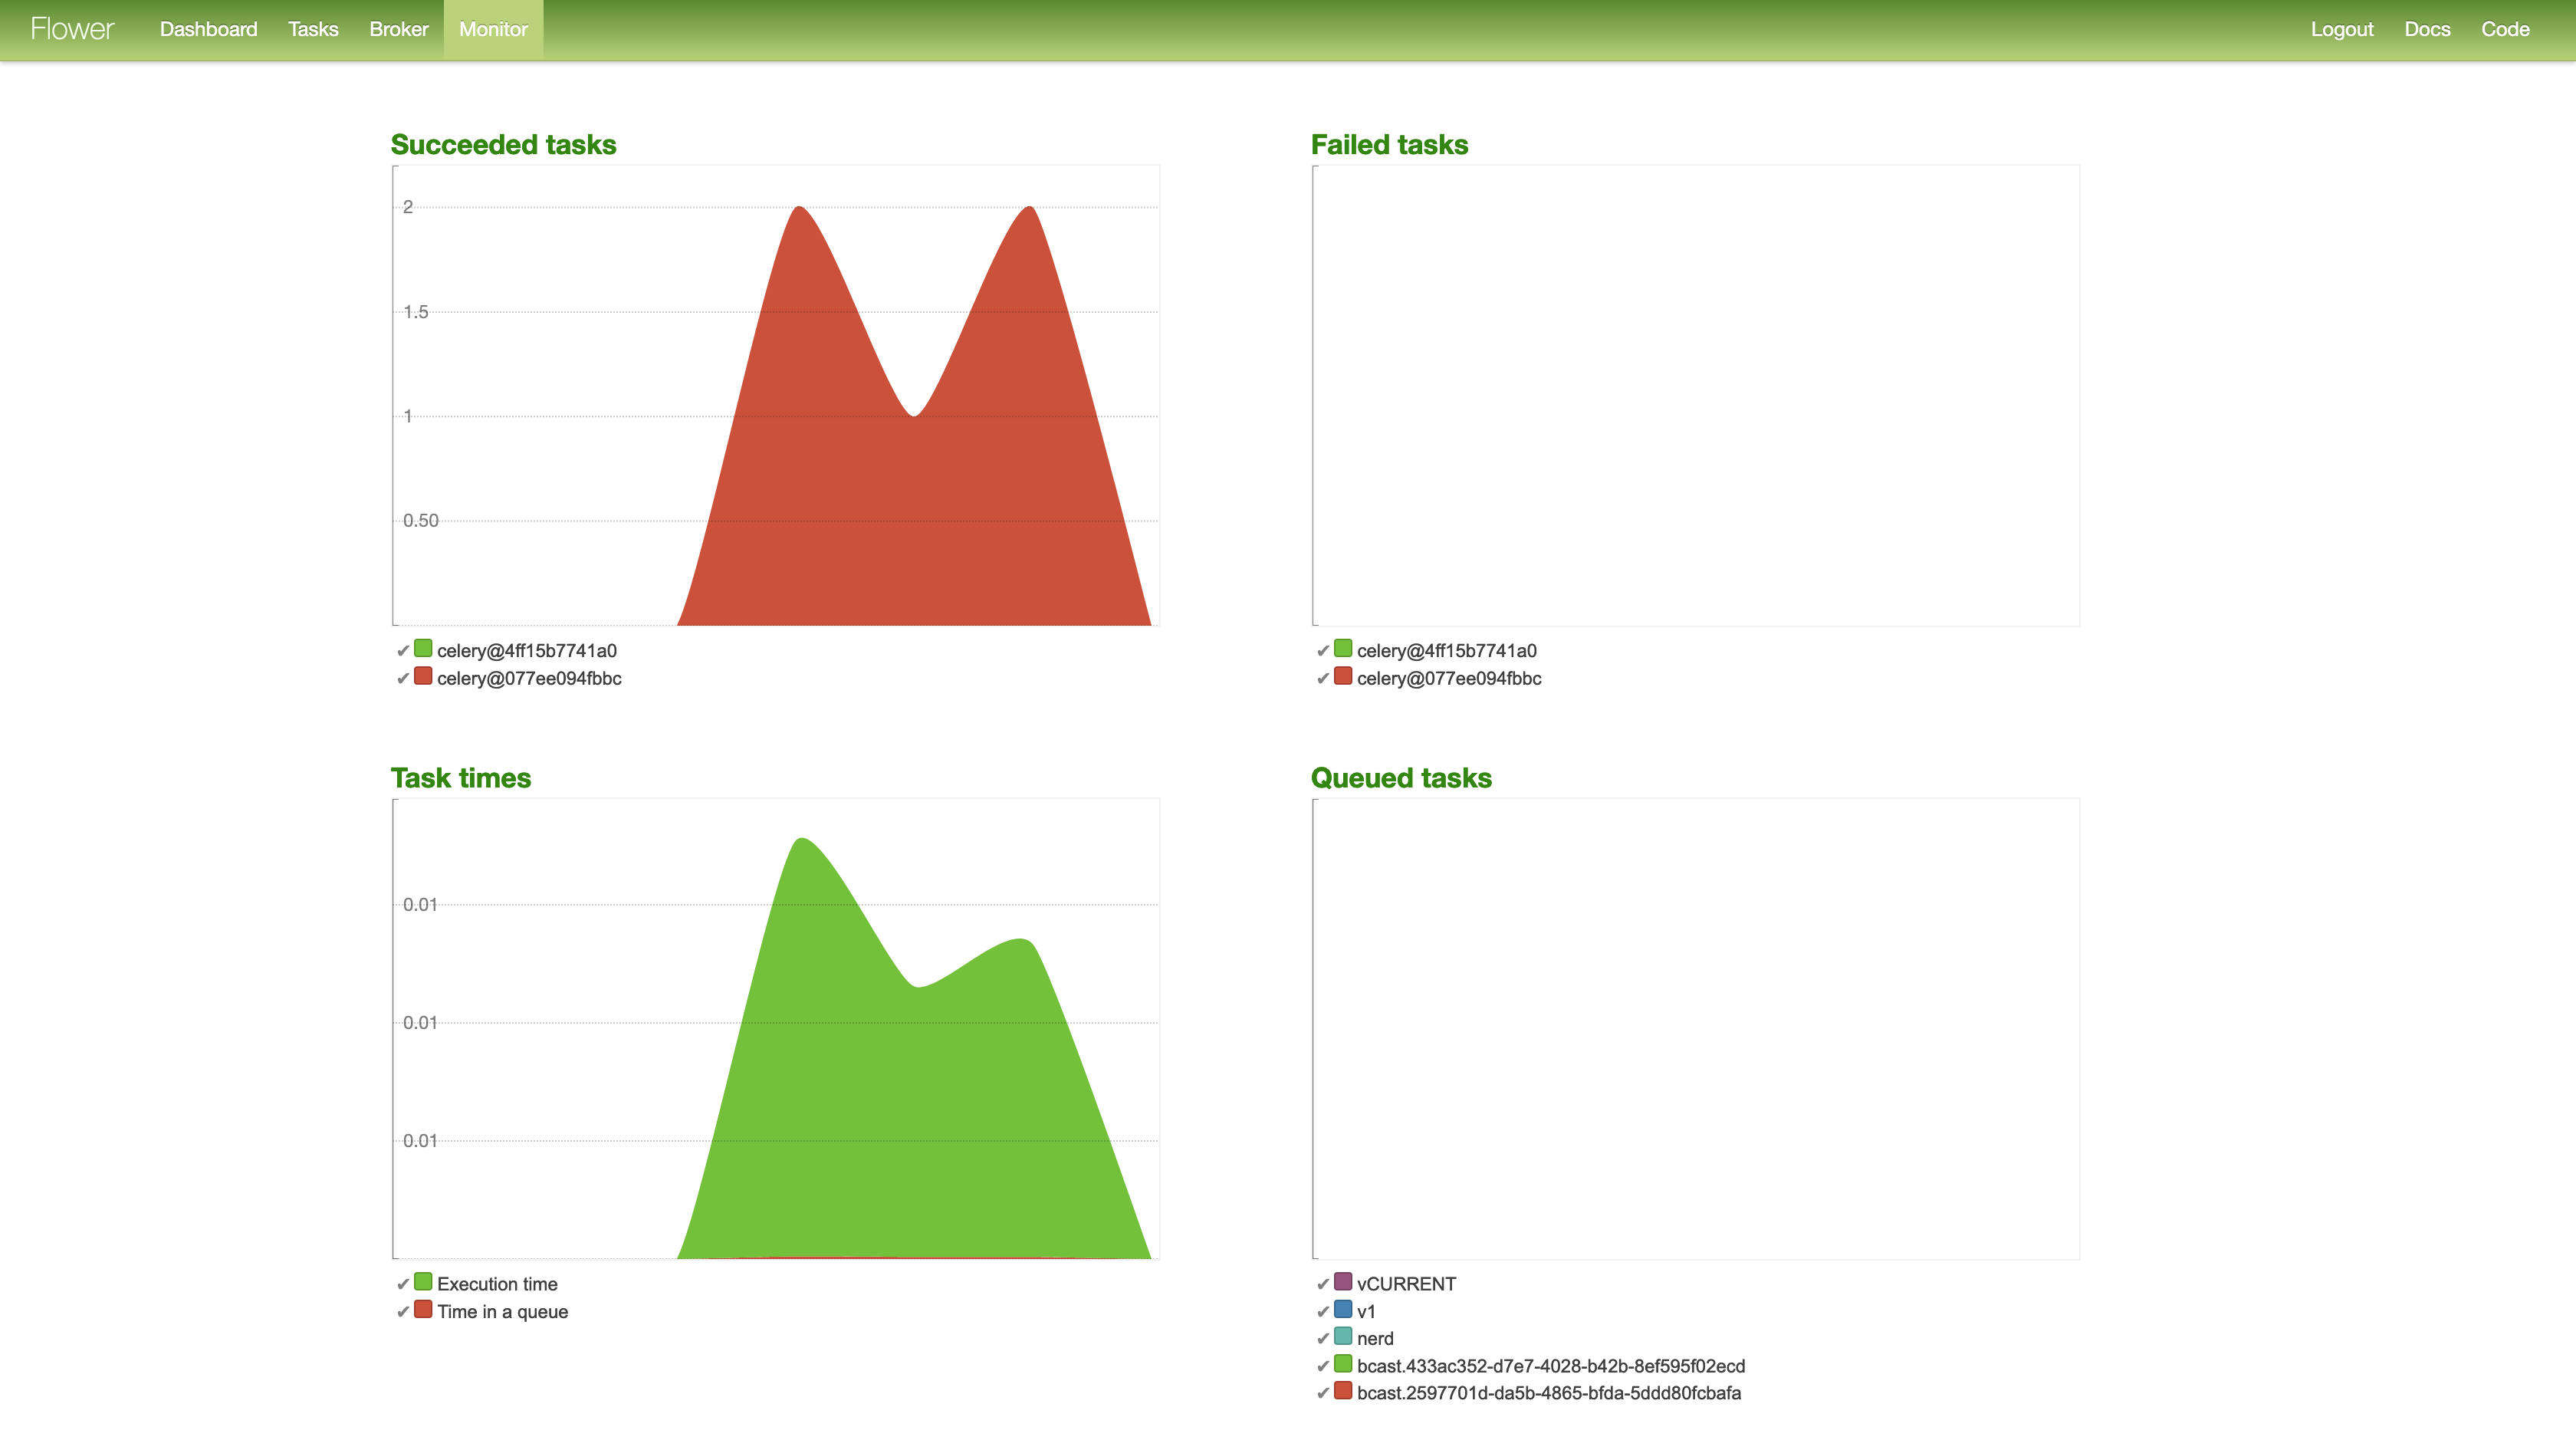
\includegraphics{assets/developer/flower-monitoring.png} 

}

\caption{Monitoreo en tiempo real en Flower.}\label{fig:developer-flower-monitoring}
\end{figure}

\begin{figure}[H]

{\centering 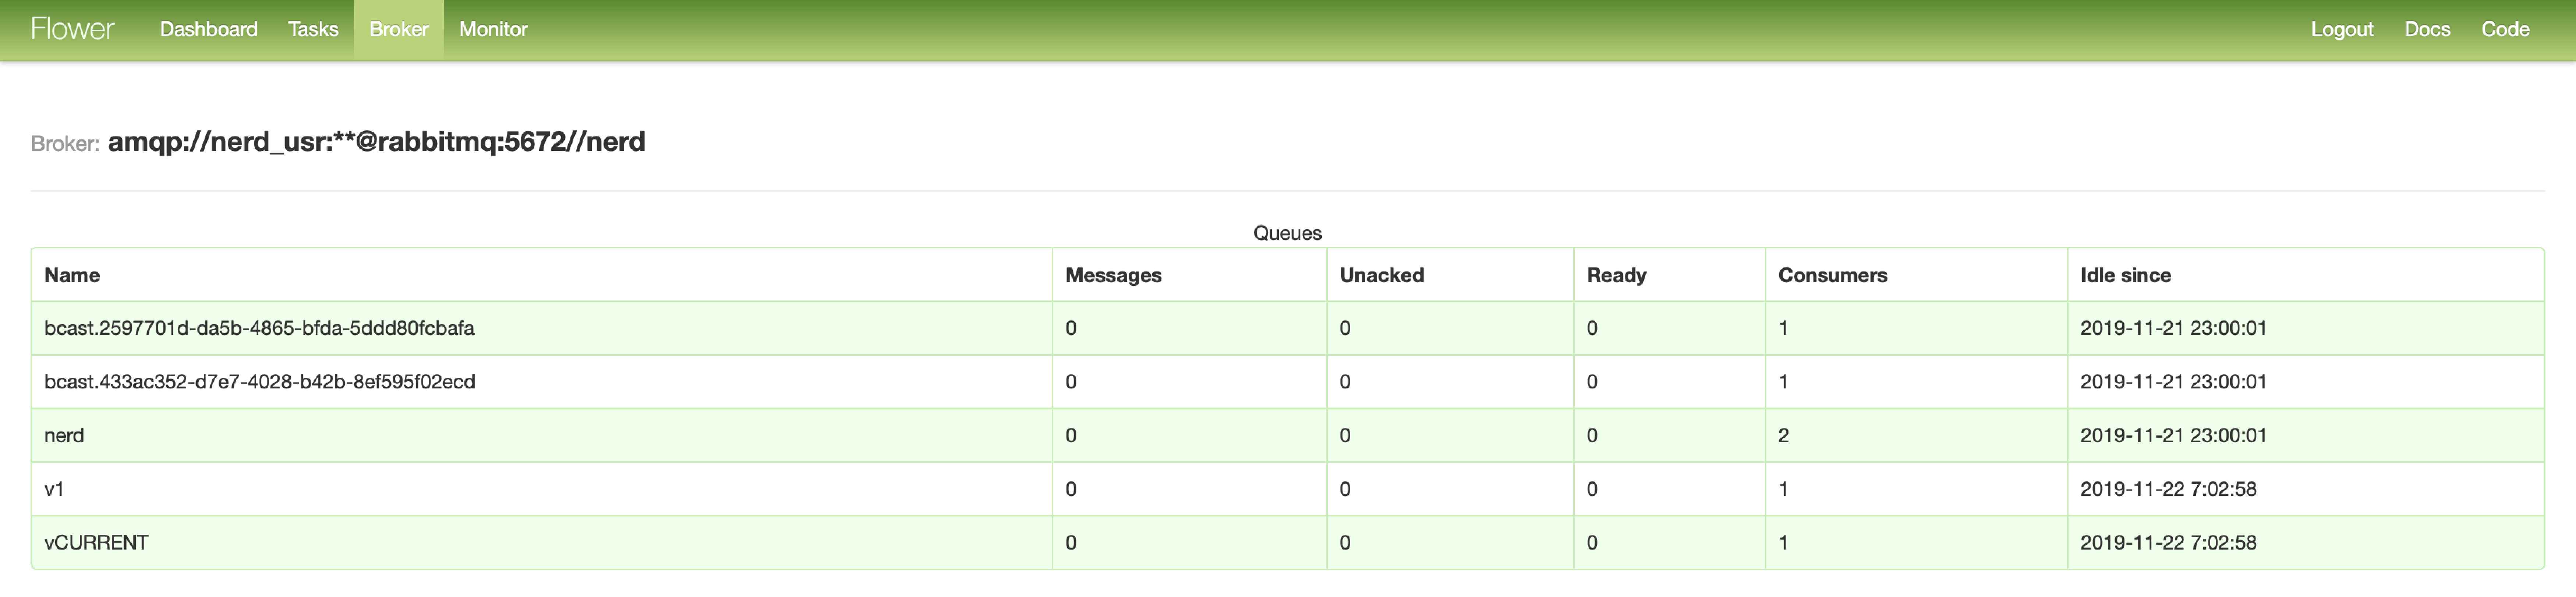
\includegraphics{assets/developer/flower-broker.pdf} 

}

\caption{Listado de colas activas en Flower.}\label{fig:developer-flower-broker}
\end{figure}

\begin{figure}[H]

{\centering 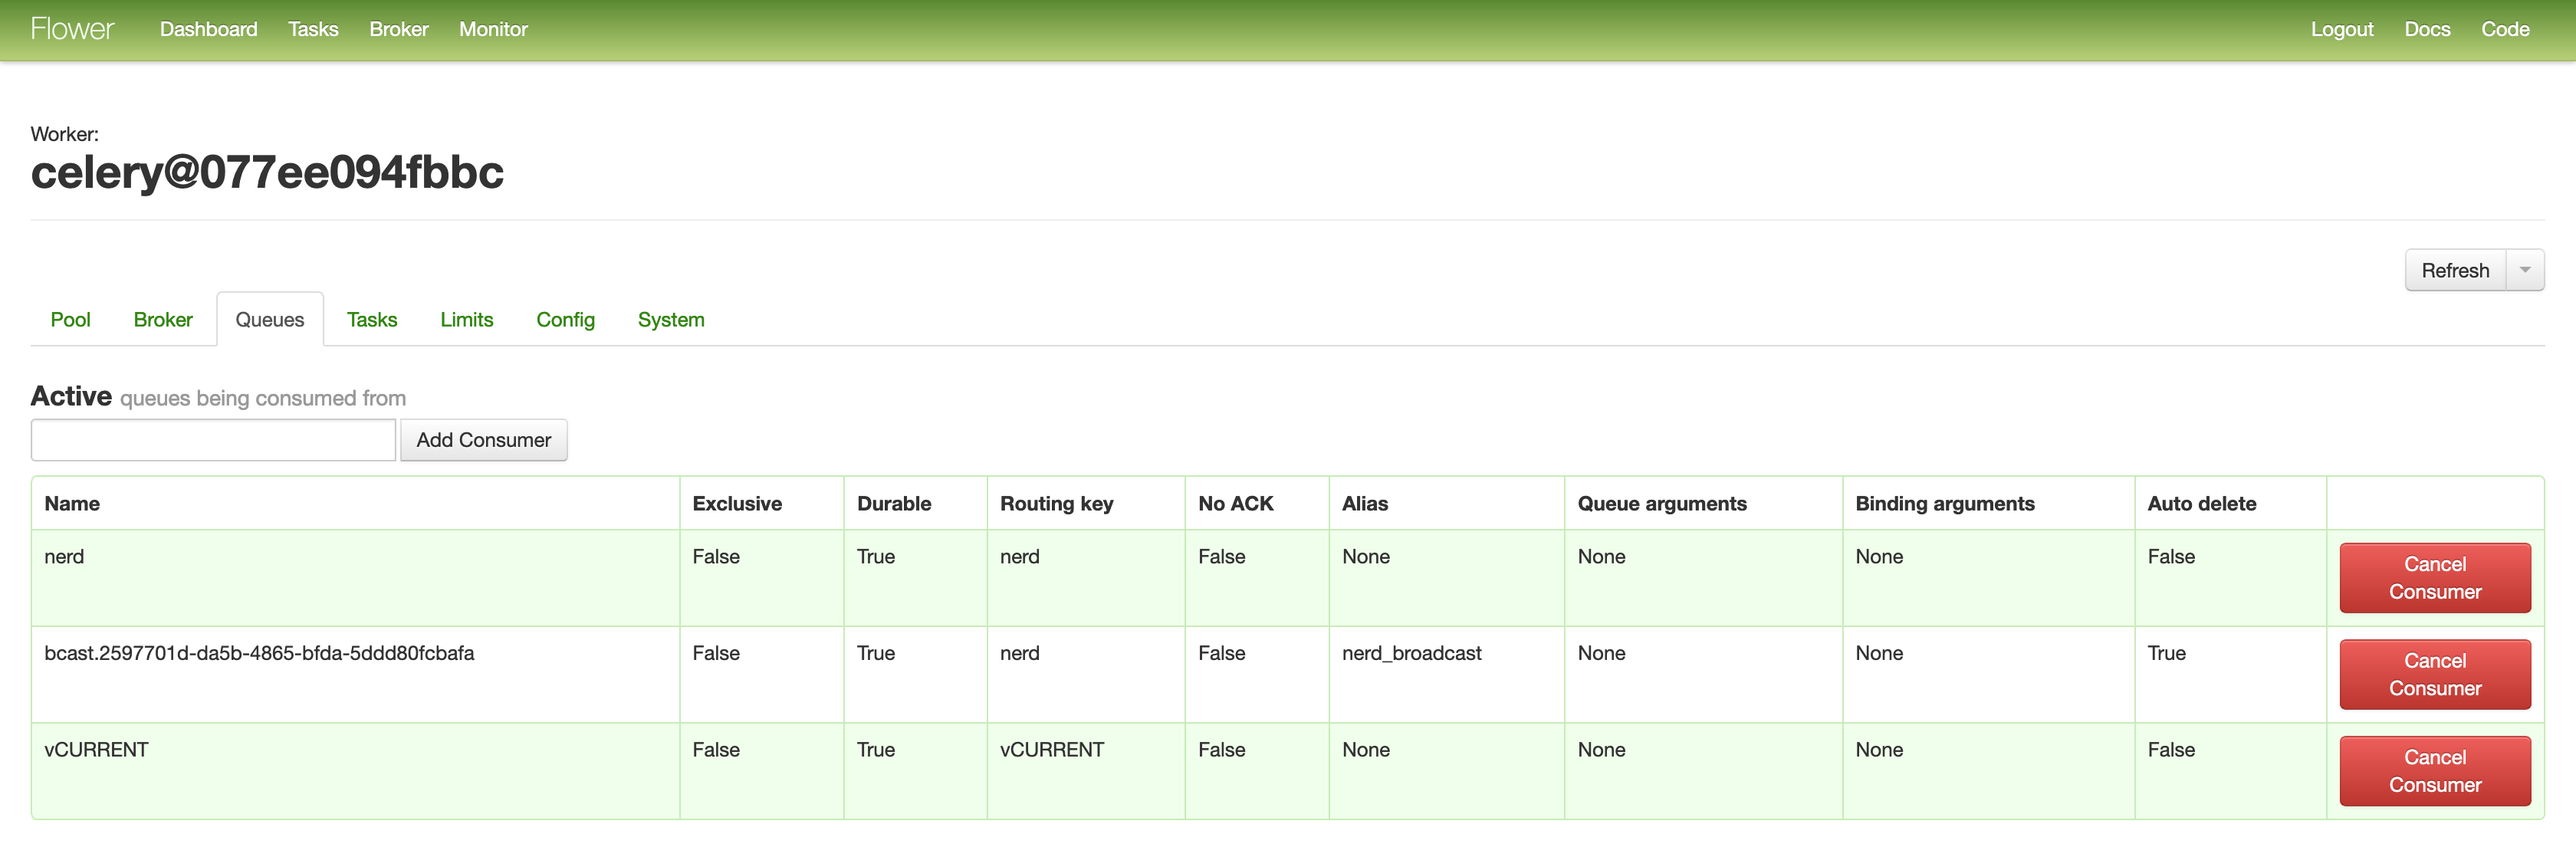
\includegraphics{assets/developer/flower-worker-queues.png} 

}

\caption{Colas de mensaje escuchadas por un worker.}\label{fig:developer-flower-worker-queues}
\end{figure}

\hypertarget{worker-1}{%
\subsubsection{Worker}\label{worker-1}}

El proceso de \emph{worker} fue implementado en \emph{Python} utilizando la librería \emph{Celery}.

Deben tener por diseño siempre un modelo de inferencia de \emph{spaCy} cargado en memoria, por lo que cuando se crea uno nuevo, se le asigna por defecto el \emph{snapshot} actual (\texttt{snapshot\_id\ =\ 0}) para poder ayudar a distribuir la carga de los pedidos al \emph{API}.

Debido a que requieren de un \emph{snapshot} para poder realizar la tarea de \emph{NER} así como también requieren del \emph{corpus} etiquetado para poder entrenar el modelo, cada \emph{worker} debe tener acceso a la base de datos principal de \emph{NERd} (Figura \ref{fig:process-overview-client}).

Cada \emph{worker} puede realizar las siguientes tareas:

\begin{itemize}
\tightlist
\item
  \textbf{train}: Entrenar el modelo de inferencia de \emph{spaCy} utilizando el snapshot para el cual fue configurado.
\item
  \textbf{un\_train}: Borra el modelo guardado en el disco, efectivamente \enquote{des-entrenandose}. Principalmente utilizado para liberar recursos.
\item
  \textbf{reload}: Recarga el modelo de inferencia desde el disco. Utilizado cuando algún worker entrenó el modelo y el actual quedó desactualizado.
\item
  \textbf{nlp}: Realiza la tarea de \emph{NER} utilizando el modelo cargado.
\item
  \textbf{change\_snapshot}: Cambia el \emph{snapshot} utilizado en el worker.
\end{itemize}

\hypertarget{vista-fuxedsica}{%
\subsection{Vista física}\label{vista-fuxedsica}}

\begin{quote}
La vista física representa el sistema desde el punto de vista de un ingeniero de sistemas.
Se refiere a la topología de los componentes de software en la capa física, así como a las conexiones físicas entre estos componentes.
Esta vista también se conoce como la vista de \emph{deployment}.
\end{quote}

Para la implementación de cada una de las partes de \emph{NERd}, tuvimos como primer objetivo lograr el desarrollo de un proyecto que pudiera escalar horizontalmente desde su concepción, es por ello que separamos cada parte del proyecto para poder lograr una arquitectura que escale naturalmente.

\hypertarget{docker}{%
\subsubsection{\texorpdfstring{\emph{Docker}}{Docker}}\label{docker}}

\emph{Docker} (``Docker,'' \protect\hyperlink{ref-docker}{2019}) es un conjunto de productos que permiten empaquetar aplicaciones en contenedores. Cada contenedor contiene todo lo necesario para que la aplicación funcione (código, dependencias, configuraciones, herramientas del sistema, etc.)\footnote{\url{https://www.docker.com/resources/what-container}}. Mediante el uso de virtualización, es posible distribuir y ejecutar un contenedor en más de un sistema, lo que lleva a la posibilidad de tener varias réplicas de un mismo servicio ejecutando al mismo tiempo.

Por ésta razón decidimos utilizar \emph{Docker} como la herramienta para empaquetar los servicios principales de \emph{NERd}.

La implementación completa de \emph{NERd} está formada por 5 contenedores requeridos y uno opcional:

\begin{itemize}
\tightlist
\item
  \textbf{app}: Contiene el servicio de \emph{API}.
\item
  \textbf{mongodb}: Contiene la base de datos.
\item
  \textbf{rabbitmq}: Contiene la cola de mensajes.
\item
  \textbf{ui}: Contiene la página \emph{web} de administración y entrenamiento.
\item
  \textbf{worker}: Contiene a uno o más \emph{workers}.
\item
  \textbf{flower}: Contiene el servicio de monitoreo de \emph{Flower} (Opcional).
\end{itemize}

\hypertarget{deployment-docker-images}{%
\subsubsection{\texorpdfstring{Deployment: \emph{Docker images}}{Deployment: Docker images}}\label{deployment-docker-images}}

Para realizar un \emph{deployment} de nuevas versiones de cada contenedor de docker, existen comandos dentro del archivo \texttt{Makefile}:

\begin{Shaded}
\begin{Highlighting}[]
\FunctionTok{make}\NormalTok{ build }\CommentTok{# Construye nuevas imágenes para cada uno de los servicios}
\FunctionTok{make}\NormalTok{ release-push }\CommentTok{# Publica las nuevas imágenes a github}
\end{Highlighting}
\end{Shaded}

\hypertarget{deployment-service}{%
\subsubsection{Deployment: Service}\label{deployment-service}}

Para poder crear un entorno completo de \emph{NERd}, utilizamos una herramienta incluída en \emph{Docker} llamada \emph{Docker Compose} (``Docker compose,'' \protect\hyperlink{ref-dockercompose}{2019}), con la cual definimos cada uno de los servicios y las conexiones de red y disco necesarias entre cada contenedor de manera tal que las conexiones mostradas en la figura \ref{fig:physical-overview} funcionen correctamente.

A su vez, dentro de un archivo \emph{Makefile} del proyecto definimos un conjunto de comandos que sirven para levantar un entorno de desarrollo de \emph{NERd}.

\begin{Shaded}
\begin{Highlighting}[]
\FunctionTok{make}\NormalTok{ setup }\CommentTok{# Inicializa todos los contenedores de NERd, creando 2 workers}
\FunctionTok{make}\NormalTok{ down }\CommentTok{# Destruye todos los contenedores de NERd}
\FunctionTok{make}\NormalTok{ stop }\CommentTok{# Apaga los contenedores de NERd (sirve liberar recursos en una máquina)}
\FunctionTok{make}\NormalTok{ start }\CommentTok{# Enciende los contenedores parados de NERd}
\end{Highlighting}
\end{Shaded}

Para realizar un deploy de la aplicación en un entorno productivo utilizaremos de ejemplo utilizando el servidor provisto por el \emph{ITBA}.

Primero es necesario contar con una configuración de SSH la cual defina el \emph{host} \emph{pf-nerd}:

\begin{verbatim}
Host pampero
    Hostname pampero.itba.edu.ar
    User <ITBA_USER>

Host pf-nerd
    Hostname <MACHINE_IP>
    User <MACHINE_USER>
     # Requerimos un proxy para acceder a pampero
    ProxyCommand ssh pampero nc %h %p
    ControlMaster auto
    ControlPath ~/.ssh/sockets/%r@%h-%p
    ControlPersist 600
\end{verbatim}

Con esa configuración en el archivo \texttt{\textasciitilde{}/.ssh/config} podemos ejecutar el comando para realizar el setup de una instancia con las configuraciones de producción.

\begin{Shaded}
\begin{Highlighting}[]
\FunctionTok{make}\NormalTok{ prod-setup}
\end{Highlighting}
\end{Shaded}

Ese comando puede ser utilizado también para

\hypertarget{escalamiento-horizontal}{%
\subsubsection{Escalamiento horizontal}\label{escalamiento-horizontal}}

En la figura \ref{fig:physical-overview} podemos ver a los 5 contenedores principales de \emph{NERd}. Cada uno de ellos fue pensado para que con cambios tanto a sus configuraciones puedan existir varias instancias de cada uno.

\begin{figure}[H]

{\centering 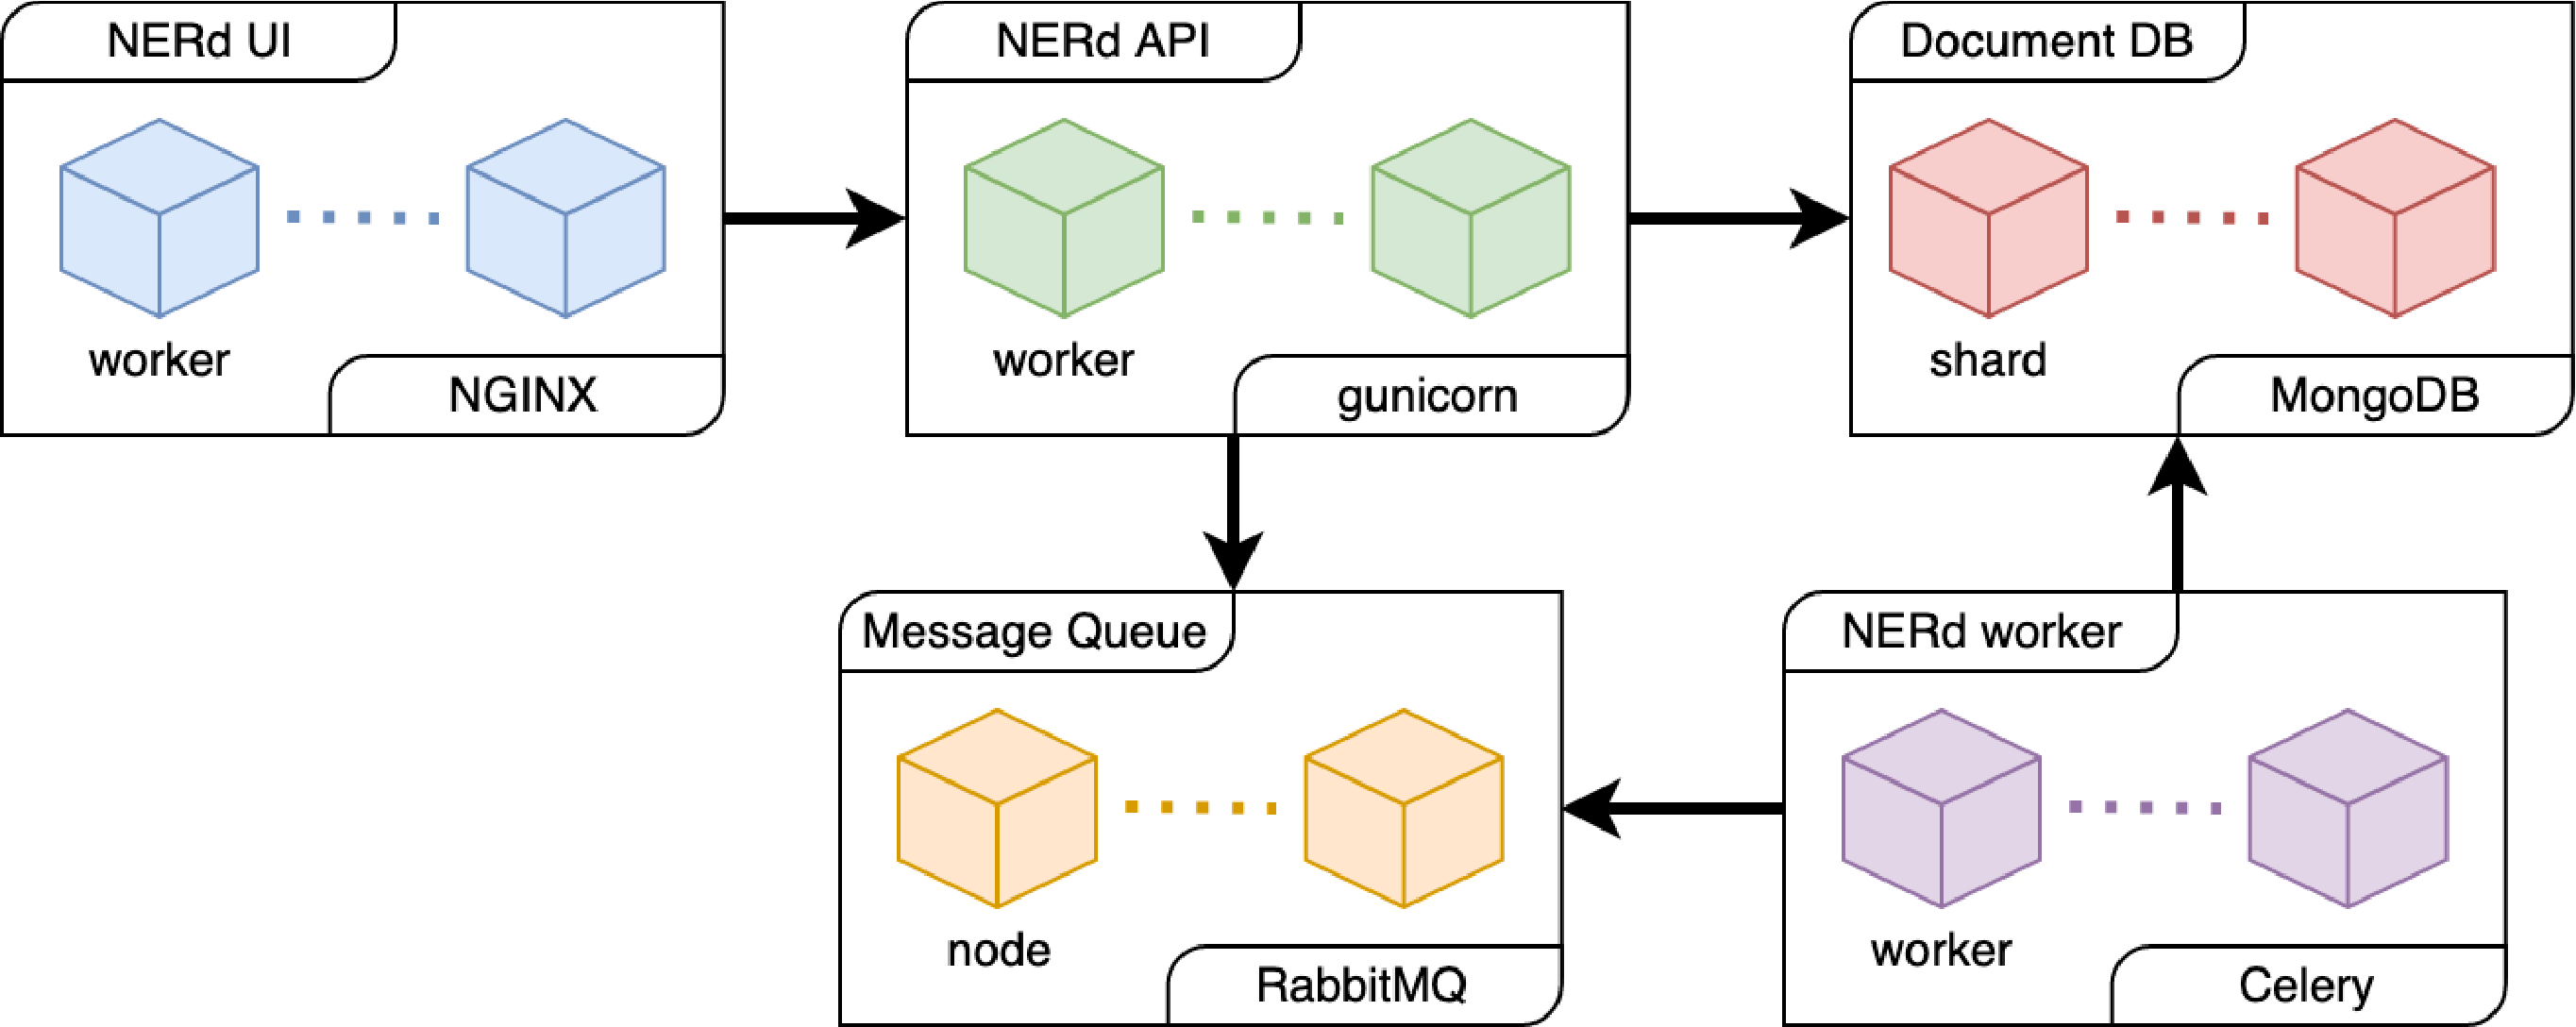
\includegraphics{assets/physical/overview.pdf} 

}

\caption{Interacción de servicios.}\label{fig:physical-overview}
\end{figure}

\hypertarget{nerd-cluster}{%
\paragraph{\texorpdfstring{\emph{NERd cluster}}{NERd cluster}}\label{nerd-cluster}}

Debido a que el \emph{API} consume sus datos de \emph{MongoDB} así como también requiere de una conexión mediante \emph{Celery} a \emph{RabbitMQ} para poder realizar las tareas de \emph{NER}, es posible tener varias instancias del mismo de manera tal que cada una se conecte al cluster de los dos servicios. Es posible mediante el uso de un \emph{Load Balancer} generar un cluster de servicios de \emph{API}.

\hypertarget{rabbitmq-cluster}{%
\paragraph{\texorpdfstring{\emph{RabbitMQ cluster}}{RabbitMQ cluster}}\label{rabbitmq-cluster}}

\emph{RabbitMQ} está pensado desde su concepción para poder escalar horizontalmente\footnote{\url{https://www.rabbitmq.com/clustering.html}}, por lo que para tener varias instancias de cola de mensajes será necesario corregir la configuración del servicio.

\hypertarget{mongodb-cluster}{%
\paragraph{\texorpdfstring{\emph{MongoDB cluster}}{MongoDB cluster}}\label{mongodb-cluster}}

Al igual que \emph{RabbitMQ}, \emph{MongoDB} fue diseñado para escalar horizontalmente (ver \protect\hyperlink{MongoDBDev}{Base de datos}), por lo que para poder escalar horizontalmente la base de datos será necesario modificar la configuración del contenedor para que forme parte de un cluster.

\hypertarget{worker-cluster}{%
\paragraph{\texorpdfstring{\emph{Worker cluster}}{Worker cluster}}\label{worker-cluster}}

Dado que cada \emph{worker} está implementado como un \emph{Celery worker}, mientras la configuración del mismo sea correcta, al levantar nuevos containers será posible escalarlo horizontalmente. Incluído en el repositorio de \emph{NERd} está un comando de \emph{Makefile} que permite escalar el servicio worker:

\begin{Shaded}
\begin{Highlighting}[]
\FunctionTok{make}\NormalTok{ scale-up }\CommentTok{# Crea un nuevo worker localmente}
\FunctionTok{make}\NormalTok{ scale-down }\CommentTok{# Destruye un worker localmente}
\end{Highlighting}
\end{Shaded}

\hypertarget{escenarios}{%
\subsection{Escenarios}\label{escenarios}}

\begin{quote}
La descripción de una arquitectura se ilustra utilizando un pequeño conjunto de casos de uso, o escenarios, que se convierten en una quinta vista.
Los escenarios describen secuencias de interacciones entre objetos y entre procesos.
Se utilizan para identificar elementos arquitectónicos y para ilustrar y validar el diseño de la arquitectura.
También sirven como punto de partida para las pruebas de un prototipo de arquitectura.
Esta vista también se conoce como vista de caso de uso.
\end{quote}

\hypertarget{web-relogin}{%
\subsubsection{\texorpdfstring{\emph{Web}: \emph{relogin}}{Web: relogin}}\label{web-relogin}}

Debido a como está diseñado \emph{JWT}, se espera que los tokens de acceso sean válidos por un tiempo acotado (en nuestra implementación ese tiempo es de 15 minutos). Debido a eso, es necesario refrescar el \emph{token} de acceso utilizando el \emph{token} de \emph{refresh}.

Si el cliente tiene un \emph{token} de \emph{refresh}, en la figura \ref{fig:scenarios-relogin} podemos ver el flujo que realiza la implementación \emph{web} del entrenador para realizar el refresco de la sesión. Al recibir un \(401\) por parte del servidor, el SDK realiza un

\begin{figure}[H]

{\centering \includegraphics{nerd-pf_files/figure-latex/scenarios-relogin-1.pdf} 

}

\caption{Flujo de relogin}\label{fig:scenarios-relogin}
\end{figure}

\hypertarget{ner}{%
\subsubsection{\texorpdfstring{\emph{NER}}{NER}}\label{ner}}

Como podemos ver en la figura \ref{fig:scenarios-ner}, para realizar el reconocimiento de entidades nombradas, deben intervenir cuatro actores.

Cuando un \emph{cliente} realiza un pedido al \emph{API}, crea una nueva tarea en la cola correspondiente al snapshot especificado por la versión en el \emph{request} en \emph{RabbitMQ}. Luego, un único \emph{worker} que esté escuchando la cola para esa versión va a tomar la tarea, realizar la tarea de inferencia y asignarle un resultado a esa tarea. Finalmente, \emph{RabbitMQ} notifica al \emph{API} de la tarea y este puede devolver finalmente el resultado al \emph{Cliente}.

\begin{figure}[H]

{\centering \includegraphics{nerd-pf_files/figure-latex/scenarios-ner-1.pdf} 

}

\caption{Flujo de NER.}\label{fig:scenarios-ner}
\end{figure}

\hypertarget{web-entrenador-web}{%
\subsubsection{\texorpdfstring{\emph{Web}: Entrenador web}{Web: Entrenador web}}\label{web-entrenador-web}}

Como podemos ver en la figura \ref{fig:scenarios-web-train}, para poder mostrar un texto a entrenar son necesarios cinco servicios.

El proceso de la inferencia es el mismo que el mostrado en la figura \ref{fig:scenarios-ner}, agregándose la consulta a \emph{MongoDB} al principio para poder obtener un texto que aún no haya sido entrenado por el usuario logueado.

\begin{figure}[H]

{\centering \includegraphics{nerd-pf_files/figure-latex/scenarios-web-train-1.pdf} 

}

\caption{Pedido de texto para entrenamiento.}\label{fig:scenarios-web-train}
\end{figure}

\hypertarget{worker-entrenamiento-y-carga-del-modelo-de-spacy}{%
\subsubsection{\texorpdfstring{\emph{Worker}: Entrenamiento y carga del modelo de spaCy}{Worker: Entrenamiento y carga del modelo de spaCy}}\label{worker-entrenamiento-y-carga-del-modelo-de-spacy}}

Dado que pueden haber varios \emph{workers} utilizando el mismo modelo de \emph{spaCy}, es de vital importancia que si existe al menos un \emph{worker} leyendo un modelo desde el disco y otro worker quiere entrenar ese modelo, que no pueda hasta que el resto haya terminado de leerlo.
Ésto se debe a que si el \emph{worker} que está entrenando el modelo sobreescribe los archivos del disco mientras otro los está leyendo, va a llevar a llevar a la falla del \emph{worker} de lectura. Como no hay ninguna limitación en la lectura, más de un \emph{worker} puede leer en simultáneo.

Para realizar ese control de concurrencia utilizamos el campo \texttt{semaphore} del modelo de \emph{snapshot} guardado en la base de datos (Figura \ref{fig:developer-db-snapshot}) el cual usualmente se encuentra en \(0\). El semáforo es incrementado en uno cuando un worker comienza a leer o termina de entrenar el modelo; es decrementado en uno cuando termina de leer o comienza a entrenar el modelo. Con esas cuatro acciones es posible controlar la correcta lectura/escritura del modelo desde el disco en un entorno distribuido sin causar problemas de concurrencia.

En la figura \ref{fig:scenarios-worker-train} podemos ver un escenario en el que tanto \emph{Worker 2} y \emph{Worker 3} pueden leer en simultáneo el modelo pero \emph{Worker 1} debe quedarse esperando hasta que el semáforo vuelva a cero (nadie leyendo o entrenando el modelo) para poder realizar la tarea de entrenamiento.

\begin{figure}[H]

{\centering \includegraphics{nerd-pf_files/figure-latex/scenarios-worker-train-1.pdf} 

}

\caption{Bloqueo de entrenamiento por lectura.}\label{fig:scenarios-worker-train}
\end{figure}

\hypertarget{worker-cambio-de-snapshot}{%
\subsubsection{\texorpdfstring{\emph{Worker}: cambio de snapshot}{Worker: cambio de snapshot}}\label{worker-cambio-de-snapshot}}

Como podemos ver en la figura \ref{fig:scenarios-worker-snapshot-change}, ante una tarea de reasignación de snapshot, el \emph{worker} se desuscribe de la cola de mensajes del \emph{snapshot} que está escuchando actualmente y se suscribe a la cola de mensajes del \emph{snapshot} al que se lo quiere cambiar. Luego, se recarga el modelo.

\begin{figure}[H]

{\centering \includegraphics{nerd-pf_files/figure-latex/scenarios-worker-snapshot-change-1.pdf} 

}

\caption{Cambio de modelo.}\label{fig:scenarios-worker-snapshot-change}
\end{figure}

\newpage

\hypertarget{results}{%
\section{Resultados de entrenamiento}\label{results}}

\hypertarget{muxe9trica-valor-f}{%
\subsection{Métrica: Valor-F}\label{muxe9trica-valor-f}}

En análisis estadístico de clasificación binaria, el \(\text{valor-F}\) es una medida de la \textbf{exactitud} de una prueba.
Considera tanto la \textbf{precisión} (del inglés \emph{precision}) como la \textbf{exhaustividad} (del ingles \emph{recall}). Su fórmula es la siguiente:

\[
F_\beta = (1 + \beta^2) \cdot \frac{\mathrm{precision} \cdot \mathrm{recall}}{(\beta^2 \cdot \mathrm{precision}) + \mathrm{recall}}
\]

En particular cuando \(F_1\) (\(\beta = 1\)) es la media armónica de la precisión y la exhaustividad, donde un puntaje \(F_1\) alcanza su mejor valor en 1 (precisión y \emph{recall} perfecta) y el peor en 0.

\[
F_1 = \left(\frac{2}{\mathrm{recall}^{-1} + \mathrm{precision}^{-1}}\right) = 2 \cdot \frac{\mathrm{precision} \cdot \mathrm{recall}}{\mathrm{precision} + \mathrm{recall}}
\]

Donde

\begin{itemize}
\tightlist
\item
  \(\text{precision}\) es el número de resultados positivos correctos dividido por el número de todos los resultados positivos devueltos por el clasificador.
  En particular para nuestro uso es el número de entidades nombradas que coinciden exactamente con el conjunto de evaluación.
  Por ejemplo, cuando se predice \texttt{{[}Persona\ Horacio{]}\ {[}Persona\ Gómez{]}}, pero lo correcto era \texttt{{[}Persona\ Horacio\ Gómez{]}}, la precisión es cero. La precisión es después promediada por cada una de la entidades nombradas.
\end{itemize}

\[
\text{precision}=\frac{|\{\text{resultados positivos}\}\cap\{\text{resultados correctos}\}|}{|\{\text{resultados positivos}\}|}
\]

\begin{itemize}
\tightlist
\item
  \(\text{recall}\) es el número de resultados positivos correctos dividido por el número todas las muestras que deberían haberse identificado como positivas.
  En nuestro uso es el número de entidades del conjunto de evaluación que aparecen exactamente en la misma posición en las predicciones.
\end{itemize}

\[
\text{recall}=\frac{|\{\text{resultados positivos}\}\cap\{\text{resultados correctos}\}|}{|\{\text{resultados correctos}\}|}
\]

La métrica de \(\text{valor-F}\) es ampliamente utilizada en la literatura del procesamiento de lenguaje natural \emph{NLP} (Hand \& Christen, \protect\hyperlink{ref-pub_1084928040}{2018}); y en especial en el ámbito del reconocimiento de entidades nombradas \emph{NER}.

Por esa razón hemos decidido utilizar la métrica \(F_1\) para poder comparar nuestra \textbf{exactitud} con los resultados obtenidos por los entrenamientos de otras publicaciones y sistemas.

\hypertarget{result-data}{%
\subsection{Resultados obtenidos}\label{result-data}}

La recomendación de \emph{spaCy} para entrenamientos de \emph{NER} es de al menos etiquetar 2000 textos, por lo que en este trabajo hemos etiquetado utilizando nuestra plataforma un número suficiente como para poder utilizar en el cálculo de resultados una \textbf{muestra aleatoria} de 4000 valores.

En los entrenamientos por refuerzo es necesario tomar la decisión de cuantos textos etiquetados serán utilizados para entrenar y cuantos serán utilizados para evaluar el entrenamiento.

Decidimos realizar diferentes pruebas y combinaciones de cantidad de documentos de entrenamiento y evaluación para analizar el \(\text{valor-F}\) del modelo resultante:

\begin{itemize}
\tightlist
\item
  Entrenamiento: 0\% (0 documentos) y evaluación: 0\% (4000). Este escenario equivale a utilizar el modelo base de spaCy.
\item
  Entrenamiento: 50\% (2000 documentos) y evaluación: 50\% (2000).
\item
  Entrenamiento: 75\% (3000 documentos) y evaluación: 25\% (1000).
\item
  Entrenamiento: 80\% (3200 documentos) y evaluación: 20\% (800).
\item
  Entrenamiento: 85\% (3400 documentos) y evaluación: 15\% (600).
\item
  Entrenamiento: 90\% (3600 documentos) y evaluación: 10\% (400).
\end{itemize}

En la figura \ref{fig:fig-boxplot} se puede ver que nuestro sistema alcanza una exactitud en \(\text{valor-F}\) de aproximadamente 80 puntos con relativamente pocos documentos.

\begin{figure}[H]

{\centering \includegraphics[width=0.8\linewidth]{nerd-pf_files/figure-latex/fig-boxplot-1.pdf} 

}

\caption{Boxplot del Valor-F vs vantidad de documentos de entrenamiento}\label{fig:fig-boxplot}
\end{figure}

Sobre la cantidad de documentos necesarios para el entrenamiento vs evaluación podemos concluir que una relación 85\% / 15\% es la más acertada para un conjunto de \(4000\) documentos.

\newpage

\hypertarget{discussion}{%
\section{Discusión}\label{discussion}}

\hypertarget{analisis-de-resultados}{%
\subsection{Analisis de resultados}\label{analisis-de-resultados}}

Los resultados indicados en la sección \ref{result-data} muestran que el \(\text{valor-F}\) inicial de \emph{spaCy} para nuestro \emph{corpus} de noticias tiene una \emph{score} de 66 puntos. Esta puntuación dista mucho del valor 89 que indica la librería en su documentación (Honnibal \& Montani, \protect\hyperlink{ref-spacy-spanish-model}{2019}) para este idioma.

La razón de esta discrepancia ha sido mencionada en varias oportunidades a lo largo de este trabajo; el modelo de \emph{spaCy} ha sido entrenado con un \emph{corpus} de documentos diferente del que nosotros como usuarios de la librería tenemos interés. En particular el modelo inicial de \emph{spaCy} ha sido entrenado con la siguiente información:

\begin{itemize}
\tightlist
\item
  \textbf{\emph{Spanish UD AnCora Corpus}}. Contiene más de 14mil documentos de entrenamiento provenientes de noticias españolas (Zeman \& Martínez Alonso, \protect\hyperlink{ref-ancora-es}{2019}).
\item
  \textbf{\emph{WikiNER}}. Proveniente de más de 50,000 documentos de wikipedia en español (Nothman, Ringland, Radford, Murphy, \& Curran, \protect\hyperlink{ref-Nothman2017}{2017}).
\end{itemize}

Este es un claro ejemplo de la fragilidad que poseen los modelos estadísticos en cuanto al corpus de interés. El modelo de \emph{spaCy} ha sido entrenado con noticias de España, sin embargo, esas noticias no alcanzan para que el modelo pueda generalizar a las noticias de Argentina y mantener el alto grado de exactitud del modelo anterior.

En este trabajo entrenando sobre el modelo de \emph{spaCy} con 3600 documentos hemos alcanzado subir ese \(\text{valor-F}\) de 66 a 80 puntos. Con una fracción de los documentos que \emph{spaCy} utilizó en su entrenamiento base podemos ajustar cualquier corpus de documentos.

\hypertarget{tipos-de-entidades}{%
\subsection{Tipos de entidades}\label{tipos-de-entidades}}

La detección de entidades por defecto en español de \emph{spaCy}, incluye las entidades \texttt{Persona}, \texttt{Organización}, \texttt{Locación} y \texttt{Misceláneo}. Cómo nuestro sistema soporta el entrenamiento de nuevas entidades tomamos la decisión de incluir un quinto tipo de entidad el de \texttt{Fecha}.

El hecho de que exista una clasificación de entidad como \texttt{Misceláneo} indica que hay otro tipo de entidades que no están siendo clasificadas específicamente y entran en esta categoría genérica. En la sección \ref{ner-formal} se define formalmente que es una entidad, por lo que se puede inferir que toda entidad nombrada que cumpla la definición formal y no posea un tipo de entidad específicamente definido entra en la categoría de entidad Miscelanea.

Existe literatura acerca de la posible taxonomía de las entidades. En (Brunstein, \protect\hyperlink{ref-brunstein2002}{2002}) se proponen 29 tipos y 64 subtipos.

Esta discusión es producto de la necesidad de agregar nuevos tipos que experimentamos al finalizar el entrenamiento de las 4000 noticias. Sin embargo lo propuesto en (Brunstein, \protect\hyperlink{ref-brunstein2002}{2002}) no cubrió nuestras expectativas. Finalmente encontramos una taxonomía lo suficientemente completa para cubrir nuestras necesidades (Sekine, \protect\hyperlink{ref-Sekine-NER}{2007}) que puede ser resumida en la figura \ref{fig:fig-sekine}.

\begin{figure}[H]

{\centering \includegraphics{assets/sekine.pdf} 

}

\caption{Taxonomía extendida de Sekine.}\label{fig:fig-sekine}
\end{figure}

Haciendo un análisis de dicha taxonomía encontramos que nuestro \emph{corpus} puede beneficiarse de los siguientes nuevos tipos de entidad:

\begin{itemize}
\tightlist
\item
  \textbf{\emph{Political\_Party}}: diferentes actores políticos.

  \begin{itemize}
  \tightlist
  \item
    ej: peronistas, kirchneristas, macristas.
  \end{itemize}
\item
  \textbf{\emph{Offence}}: ofensas.

  \begin{itemize}
  \tightlist
  \item
    ej: asesinato, abducción, fraude, aborto, robo.
  \end{itemize}
\item
  \textbf{\emph{Facility\_Name}}: lugares específicos.

  \begin{itemize}
  \tightlist
  \item
    ej: Ecoparque, Disneyland, Canal de Suez, Aeropuerto de Ezeiza.
  \end{itemize}
\item
  \textbf{\emph{Product\_Name}}: nombres de productos.

  \begin{itemize}
  \tightlist
  \item
    ej: Galaxy S10, Fiat Toro, Manaos.
  \end{itemize}
\item
  \textbf{\emph{Game}}: nombres de juegos.

  \begin{itemize}
  \tightlist
  \item
    ej: futbol, football, basket, fortnite, ajedrez.
  \end{itemize}
\end{itemize}

\hypertarget{semilla-inicial}{%
\subsection{Semilla inicial}\label{semilla-inicial}}

Nuestro sistema ofrece al usuario una forma sencilla y ágil de entrenar modelos estadísticos y sumar nuevos tipos de entidad. Sin embargo, entrenar un nuevo tipo de entidad suele ser una tarea inicialmente lenta y difícil dado que se necesita un número mínimo de etiquetas para que la nueva entidad empiece a tener relevancia dentro del modelo y sea inferida.

Por ejemplo, suponga se quiere agregar el nuevo tipo de entidad \enquote{Droga} al modelo. Podemos estar horas etiquetando entidades hasta cruzarnos con la primera instancia de \enquote{marihuana} y luego varias etiquetas más hasta cruzarnos con \enquote{cocaína}. Además, como el sistema no conoce previamente el significado abstracto de \enquote{Droga} dichas \emph{keywords} no van a ser identificadas previamente por el etiquetador.

Una posible solución para evitar esta \enquote{curva de aprendizaje} es la de permitir al usuario definir una \enquote{semilla} de palabras clave (o \emph{keywords}) a la hora de definir un tipo nuevo:

\begin{quote}
Droga: Heroína, Cocaína, Barbitúricos, Metadona, Alcohol, Ketamina, Benzodiazopines, Anfetaminas, Tabaco, Cannabis, etc.
\end{quote}

De esta manera y gracias al proceso de \emph{word-embeddings} visto en la sección \ref{encode} el modelo puede pre-entrenarse para identificar las palabras definidas y todas aquellas que tengan un significado similar en el espacio vectorial de significados.

\hypertarget{entrenamiento-live-vs-offline}{%
\subsection{\texorpdfstring{Entrenamiento \emph{live} vs \emph{offline}}{Entrenamiento live vs offline}}\label{entrenamiento-live-vs-offline}}

Existen dos maneras de entrenar un modelo de predicción NLP:

\begin{itemize}
\tightlist
\item
  \emph{Online} o \emph{Live}: cada nueva etiqueta que entrenamos es inmediatamente inyectada al modelo de predicciones.
\item
  \emph{Offline}: cada nueva etiqueta que entrenamos es guardada para ser entrenada en otro momento.
\end{itemize}

En nuestro sistemas hemos elegido la segunda opción porque al poseer la capacidad de escalar horizontalmente la cantidad de \emph{workers}; el modelo se carga en varios servicios y de ser entrenado de manera \emph{live} el entrenamiento iría a workers diferentes resultando en inconsistencias entre ellos. Existen maneras de migrar nuestro sistema a un modelo \emph{online} y mantener la capacidad de escalar horizontalmente, pero escapa al alcance que decidimos darle a este trabajo por lo cual lo consideramos una propuesta de mejora a futuro.

Uno de los mayores beneficios de tener un modelo online, ademas del trivial de que esta constantemente actualizado con las ultimas mejoras; es el de la capacidad de apuntar a los \emph{tokens} que poseen una mayor incertidumbre. En la sección \ref{use-of-cnn} hemos mencionado que puede ocurrir que algunas palabras tengan una incerteza acerca de qué etiqueta debe ser predecida. En particular este tipo de técnicas están dentro de la literatura conocida como \emph{\enquote{Uncertainty sampling}} que se puede resumir en buscar entidades que tengan un \emph{score} \(~ 0.5\) y dirigir el entrenamiento a esos \emph{tokens} primero.

\hypertarget{linkeo-de-entidades-con-knowledge-base}{%
\subsection{\texorpdfstring{\emph{Linkeo} de entidades con \emph{Knowledge Base}}{Linkeo de entidades con Knowledge Base}}\label{linkeo-de-entidades-con-knowledge-base}}

Existe otra tarea en el universo de \emph{NLP} que está muy relacionada a la tarea de \emph{NER}: es la tarea de \emph{Named Entity Linking} (``Entity linking,'' \protect\hyperlink{ref-wiki_nel}{2019}).

Un corolario de la definición de \textbf{designador rígido} en la sección \ref{ner-formal} es que una misma entidad puede tener varios designadores. Por ejemplo \enquote{Lionel Messi} también puede ser referido como \enquote{Leo Messi}, \enquote{Leo}, \enquote{La Pulga}, \enquote{Lionel Andrés \enquote{Leo} Messi}, etc. Todos ellos son designadores rígidos de una misma entidad, del concepto de Messi. A este concepto abstracto de entidad se le puede asignar un identificador único dentro de una base de datos de conocimiento (\emph{knowledge base} en inglés) para luego ser utilizado en la normalización de entidades.

Ya existen \emph{knowledge bases} universales en internet. Una de las más importante y completas es \textbf{\emph{wikidata}}. El identificador de Messi es el \texttt{Q615} (``Wikidata - lionel messi,'' \protect\hyperlink{ref-wikidata_messi}{2019}).

Si al etiquetar una entidad, además de decirle a nuestro sistema de qué tipo es, sumamos la funcionalidad de indicar a que identificador de entidad corresponde, se podría luego entrenar un nuevo modelo de \emph{NEL}, separado del modelo predictor de entidades, cuya tarea exclusiva sea la de normalizar y predecir identificadores de entidades.

El sistema puede beneficiarse ya que tendría disponible, mediante \emph{Wikidata}, de una gran cantidad información adicional acerca de la entidad incluyendo, fotos, aliases, palabras clave, etc como muestra la figura \ref{fig:fig-messi}.

\begin{figure}[H]

{\centering \includegraphics{assets/wikidata_messi.pdf} 

}

\caption{Wikidata - Lionel Messi.}\label{fig:fig-messi}
\end{figure}

Desde el punto de vista del usuario, puede beneficiarse porque obtener una representación normalizada de las entidades de un texto es una tarea importante en la sumarización de las mismas. Por ejemplo en la creación de \enquote{nubes de palabras} a partir de muchos artículos, puede ocurrir que en algunos artículos hablen de \enquote{Mauricio} y en otros se hable de \enquote{Macri}; sin embargo sería necesario unificar estos dos keywords para que el ítem tenga una relevancia mayor. Se puede observar una nube de palabras generada utilizando entidades encontradas por nuestro sistema en la figura \ref{fig:fig-cloud}.

\begin{figure}[H]

{\centering \includegraphics{assets/LosPersonajesDelDia.pdf} 

}

\caption{Con NEL se sumarían Messi con Lionel y Mauricio con Macri.}\label{fig:fig-cloud}
\end{figure}

Para finalizar, un dato curioso es que a esta tarea de reconocimiento de entidades más desambiguación de las mismas se lo suele llamar \emph{NERD} (\emph{named-entity recognition and disambiguation}) al igual que nuestro proyecto \emph{NERd}; una coincidencia accidental pero que evidencia la necesidad a futuro de implementar esta mejora.

\hypertarget{utilidad-de-la-herramienta}{%
\subsection{Utilidad de la herramienta}\label{utilidad-de-la-herramienta}}

Para poner a prueba nuestra herramienta \textbf{NERd} en un entorno real participamos de la hackatón en MediaParty 2019.

\begin{quote}
\textbf{(``Hackaton,'' \protect\hyperlink{ref-hackaton2019}{2019})} es un evento de tres días en Argentina, que reúne a 2500 emprendedores, periodistas, programadores de software y diseñadores de cinco continentes para trabajar juntos para el futuro de los medios de comunicación.
Nacido de Hacks/Hackers Buenos Aires, el evento fusiona a grandes empresas como New York Times, The Guardian, Vox, ProPublica, Watchup, Neo4J o DocumentCloud y comunidades regionales de la mayor red de periodistas y desarrolladores del mundo.
\end{quote}

Participamos en conjunto con otro proyecto final en el que van a utilizar nuestra API para hacer detección de entidades en documentos PDF.

La experiencia fue muy satisfactoria, recibimos buenas críticas sobre la usabilidad de nuestra aplicación y la gran utilidad que presta a la comunidad.

Por tal motivo recibimos el primer premio de dicha hackaton (``Mención itba,'' \protect\hyperlink{ref-mediaparty2019_win}{2019})

\newpage

\hypertarget{conclusiones}{%
\section{Conclusiones}\label{conclusiones}}

\begin{itemize}
\item
  Recomendar que con 4000 documentos se puede alcanzar 80 puntos de \(\text{valor-F}\)
\item
  Cuando se enfrenta un proyecto de etiquetado de \emph{NER}, recomendamos una etapa inicial de 4000 documentos para alcanzar una exactitud razonable y poder inferir de la experiencia obtenida de los textos analizados que tipos de entidad segun la taxonomía de (Sekine, \protect\hyperlink{ref-Sekine-NER}{2007}) en la \ref{fig:fig-sekine} se necesitan agregar.
\end{itemize}

\newpage

\hypertarget{anexo-datos-de-resultados}{%
\section*{Anexo: Datos de resultados}\label{anexo-datos-de-resultados}}
\addcontentsline{toc}{section}{Anexo: Datos de resultados}

\begin{itemize}
\tightlist
\item
  \textbf{t:} porcentaje de documentos de entrenamiento.
\item
  \textbf{v:} porcentaje de documentos de validación.
\end{itemize}

\hypertarget{t-0---v-100.-baseline-spacy}{%
\subsection{\texorpdfstring{t: 0\% - v: 100\%. \emph{Baseline spaCy}}{t: 0\% - v: 100\%. Baseline spaCy}}\label{t-0---v-100.-baseline-spacy}}

\begin{verbatim}
=============================== Training stats ===============================
Training pipeline: ner
Starting with base model 'es_core_news_md'
0 training docs
4000 evaluation docs
✔ No overlap between training and evaluation data

============================== Vocab & Vectors ==============================
ℹ 0 total words in the data (0 unique)
ℹ 20000 vectors (533736 unique keys, 50 dimensions)

========================== Named Entity Recognition ==========================
ℹ 0 new labels, 0 existing labels
0 missing values (tokens with '-' label)
✔ Good amount of examples for all labels
✔ Examples without occurrences available for all labels
✔ No entities consisting of or starting/ending with whitespace

================================== Summary ==================================
✔ 5 checks passed
Training pipeline: ['ner']
Starting with base model 'es_core_news_md'
Counting training words (limit=0)
\end{verbatim}

\begin{longtable}[]{@{}llllllll@{}}
\toprule
Itn & NER Loss & NER P & NER R & NER F & Token \% & CPU WPS & GPU WPS\tabularnewline
\midrule
\endhead
1 & 0.000 & 68.147 & 64.433 & 66.238 & 100.000 & 25983 & 26538\tabularnewline
2 & 0.000 & 68.147 & 64.433 & 66.238 & 100.000 & 25436 & 25395\tabularnewline
3 & 0.000 & 68.147 & 64.433 & 66.238 & 100.000 & 25752 & 24471\tabularnewline
4 & 0.000 & 68.147 & 64.433 & 66.238 & 100.000 & 25558 & 29465\tabularnewline
5 & 0.000 & 68.147 & 64.433 & 66.238 & 100.000 & 25058 & 24053\tabularnewline
6 & 0.000 & 68.147 & 64.433 & 66.238 & 100.000 & 23921 & 25149\tabularnewline
7 & 0.000 & 68.147 & 64.433 & 66.238 & 100.000 & 24582 & 25506\tabularnewline
8 & 0.000 & 68.147 & 64.433 & 66.238 & 100.000 & 29069 & 28158\tabularnewline
9 & 0.000 & 68.147 & 64.433 & 66.238 & 100.000 & 28226 & 28367\tabularnewline
10 & 0.000 & 68.147 & 64.433 & 66.238 & 100.000 & 23585 & 23769\tabularnewline
11 & 0.000 & 68.147 & 64.433 & 66.238 & 100.000 & 24765 & 23512\tabularnewline
12 & 0.000 & 68.147 & 64.433 & 66.238 & 100.000 & 23319 & 25613\tabularnewline
13 & 0.000 & 68.147 & 64.433 & 66.238 & 100.000 & 23118 & 24513\tabularnewline
14 & 0.000 & 68.147 & 64.433 & 66.238 & 100.000 & 21962 & 28556\tabularnewline
15 & 0.000 & 68.147 & 64.433 & 66.238 & 100.000 & 24425 & 24294\tabularnewline
16 & 0.000 & 68.147 & 64.433 & 66.238 & 100.000 & 27551 & 23843\tabularnewline
17 & 0.000 & 68.147 & 64.433 & 66.238 & 100.000 & 25224 & 24975\tabularnewline
18 & 0.000 & 68.147 & 64.433 & 66.238 & 100.000 & 24002 & 25027\tabularnewline
19 & 0.000 & 68.147 & 64.433 & 66.238 & 100.000 & 24367 & 28260\tabularnewline
20 & 0.000 & 68.147 & 64.433 & 66.238 & 100.000 & 25888 & 28075\tabularnewline
21 & 0.000 & 68.147 & 64.433 & 66.238 & 100.000 & 23356 & 25695\tabularnewline
22 & 0.000 & 68.147 & 64.433 & 66.238 & 100.000 & 28023 & 27458\tabularnewline
23 & 0.000 & 68.147 & 64.433 & 66.238 & 100.000 & 27412 & 25016\tabularnewline
24 & 0.000 & 68.147 & 64.433 & 66.238 & 100.000 & 24053 & 25072\tabularnewline
25 & 0.000 & 68.147 & 64.433 & 66.238 & 100.000 & 24194 & 24086\tabularnewline
26 & 0.000 & 68.147 & 64.433 & 66.238 & 100.000 & 24531 & 24725\tabularnewline
27 & 0.000 & 68.147 & 64.433 & 66.238 & 100.000 & 24375 & 27681\tabularnewline
28 & 0.000 & 68.147 & 64.433 & 66.238 & 100.000 & 28897 & 28069\tabularnewline
29 & 0.000 & 68.147 & 64.433 & 66.238 & 100.000 & 24530 & 23338\tabularnewline
30 & 0.000 & 68.147 & 64.433 & 66.238 & 100.000 & 23058 & 27724\tabularnewline
\bottomrule
\end{longtable}

\hypertarget{t-50---v-50}{%
\subsection{t: 50\% - v: 50\%}\label{t-50---v-50}}

\begin{verbatim}
=============================== Training stats ===============================
Training pipeline: ner
Starting with base model 'es_core_news_md'
2000 training docs
2000 evaluation docs
⚠ 1 training examples also in evaluation data

============================== Vocab & Vectors ==============================
ℹ 27595 total words in the data (6197 unique)
ℹ 20000 vectors (533736 unique keys, 50 dimensions)

========================== Named Entity Recognition ==========================
ℹ 1 new label, 4 existing labels
0 missing values (tokens with '-' label)
✔ Good amount of examples for all labels
✔ Examples without occurrences available for all labels
✔ No entities consisting of or starting/ending with whitespace

================================== Summary ==================================
✔ 4 checks passed
⚠ 1 warning
Training pipeline: ['ner']
Starting with blank model 'es'
Loading vector from model 'es_core_news_md'
Counting training words (limit=0)
\end{verbatim}

\begin{longtable}[]{@{}llllllll@{}}
\toprule
Itn & NER Loss & NER P & NER R & NER F & Token \% & CPU WPS & GPU WPS\tabularnewline
\midrule
\endhead
1 & 4373.230 & 61.762 & 57.692 & 59.658 & 100.000 & 25083 & 28411\tabularnewline
2 & 2650.090 & 72.869 & 70.618 & 71.726 & 100.000 & 21033 & 22844\tabularnewline
3 & 1879.892 & 77.506 & 75.820 & 76.653 & 100.000 & 22846 & 24881\tabularnewline
4 & 1550.256 & 77.877 & 77.018 & 77.445 & 100.000 & 26894 & 22926\tabularnewline
5 & 1331.972 & 78.330 & 78.058 & 78.194 & 100.000 & 25107 & 27973\tabularnewline
6 & 1172.236 & 78.367 & 78.689 & 78.528 & 100.000 & 24348 & 28943\tabularnewline
7 & 1021.166 & 79.104 & 79.004 & 79.054 & 100.000 & 22633 & 24151\tabularnewline
8 & 891.760 & 78.931 & 78.657 & 78.794 & 100.000 & 23971 & 23087\tabularnewline
9 & 825.860 & 78.731 & 78.657 & 78.694 & 100.000 & 28811 & 27209\tabularnewline
10 & 763.561 & 78.715 & 78.815 & 78.765 & 100.000 & 23736 & 21812\tabularnewline
11 & 680.819 & 78.754 & 78.878 & 78.816 & 100.000 & 22841 & 20951\tabularnewline
12 & 579.623 & 78.504 & 78.405 & 78.454 & 100.000 & 21688 & 28305\tabularnewline
13 & 494.455 & 78.553 & 78.405 & 78.479 & 100.000 & 23598 & 22923\tabularnewline
14 & 469.631 & 78.470 & 78.247 & 78.358 & 100.000 & 21825 & 25855\tabularnewline
15 & 421.725 & 78.592 & 78.468 & 78.530 & 100.000 & 19715 & 22731\tabularnewline
16 & 410.767 & 78.439 & 78.562 & 78.501 & 100.000 & 24155 & 22225\tabularnewline
17 & 411.734 & 78.284 & 78.531 & 78.407 & 100.000 & 21843 & 21950\tabularnewline
18 & 347.546 & 78.220 & 78.689 & 78.454 & 100.000 & 22409 & 21145\tabularnewline
19 & 353.033 & 78.119 & 78.562 & 78.340 & 100.000 & 21173 & 24639\tabularnewline
20 & 260.769 & 78.238 & 78.657 & 78.447 & 100.000 & 22068 & 22087\tabularnewline
21 & 306.896 & 78.332 & 78.752 & 78.541 & 100.000 & 22042 & 20555\tabularnewline
22 & 248.995 & 78.538 & 78.909 & 78.723 & 100.000 & 20849 & 23016\tabularnewline
23 & 269.101 & 78.300 & 78.720 & 78.510 & 100.000 & 21036 & 21311\tabularnewline
24 & 237.393 & 78.228 & 78.499 & 78.363 & 100.000 & 21676 & 21239\tabularnewline
25 & 234.766 & 78.439 & 78.562 & 78.501 & 100.000 & 20906 & 22519\tabularnewline
26 & 255.452 & 78.612 & 78.562 & 78.587 & 100.000 & 20253 & 23063\tabularnewline
27 & 226.127 & 78.432 & 78.531 & 78.481 & 100.000 & 21402 & 21935\tabularnewline
28 & 181.469 & 78.327 & 78.499 & 78.413 & 100.000 & 22511 & 19438\tabularnewline
29 & 180.268 & 77.904 & 78.026 & 77.965 & 100.000 & 18335 & 22732\tabularnewline
30 & 179.335 & 78.023 & 78.121 & 78.072 & 100.000 & 22433 & 21633\tabularnewline
\bottomrule
\end{longtable}

\hypertarget{t-75---v-25}{%
\subsection{t: 75\% - v: 25\%}\label{t-75---v-25}}

\begin{verbatim}
=============================== Training stats ===============================
Training pipeline: ner
Starting with base model 'es_core_news_md'
3000 training docs
1000 evaluation docs
✔ No overlap between training and evaluation data

============================== Vocab & Vectors ==============================
ℹ 41847 total words in the data (7928 unique)
ℹ 20000 vectors (533736 unique keys, 50 dimensions)

========================== Named Entity Recognition ==========================
ℹ 1 new label, 4 existing labels
0 missing values (tokens with '-' label)
✔ Good amount of examples for all labels
✔ Examples without occurrences available for all labels
✔ No entities consisting of or starting/ending with whitespace

================================== Summary ==================================
✔ 5 checks passed
Training pipeline: ['ner']
Starting with blank model 'es'
Loading vector from model 'es_core_news_md'
Counting training words (limit=0)
\end{verbatim}

\begin{longtable}[]{@{}llllllll@{}}
\toprule
Itn & NER Loss & NER P & NER R & NER F & Token \% & CPU WPS & GPU WPS\tabularnewline
\midrule
\endhead
1 & 5543.695 & 71.399 & 66.988 & 69.124 & 100.000 & 28067 & 25575\tabularnewline
2 & 3114.421 & 78.567 & 75.483 & 76.994 & 100.000 & 26176 & 26036\tabularnewline
3 & 2519.526 & 78.806 & 77.284 & 78.038 & 100.000 & 25530 & 25766\tabularnewline
4 & 2120.064 & 79.857 & 78.829 & 79.339 & 100.000 & 25734 & 25163\tabularnewline
5 & 1922.659 & 79.624 & 78.958 & 79.289 & 100.000 & 23645 & 25299\tabularnewline
6 & 1663.921 & 79.807 & 79.858 & 79.833 & 100.000 & 26526 & 25635\tabularnewline
7 & 1532.299 & 79.448 & 79.601 & 79.524 & 100.000 & 26120 & 26210\tabularnewline
8 & 1311.481 & 79.625 & 79.215 & 79.419 & 100.000 & 25331 & 26163\tabularnewline
9 & 1233.004 & 79.588 & 79.537 & 79.562 & 100.000 & 25709 & 25557\tabularnewline
10 & 1118.481 & 79.486 & 79.537 & 79.511 & 100.000 & 25726 & 25332\tabularnewline
11 & 1031.523 & 78.968 & 78.764 & 78.866 & 100.000 & 25399 & 26109\tabularnewline
12 & 930.418 & 79.317 & 79.215 & 79.266 & 100.000 & 23443 & 24004\tabularnewline
13 & 874.136 & 79.253 & 79.151 & 79.202 & 100.000 & 22272 & 26035\tabularnewline
14 & 828.361 & 79.199 & 78.893 & 79.046 & 100.000 & 23957 & 25490\tabularnewline
15 & 708.060 & 79.199 & 78.893 & 79.046 & 100.000 & 25963 & 28166\tabularnewline
16 & 663.398 & 78.917 & 78.764 & 78.841 & 100.000 & 29668 & 27887\tabularnewline
17 & 659.681 & 78.737 & 78.636 & 78.686 & 100.000 & 24656 & 27843\tabularnewline
18 & 575.416 & 78.852 & 78.700 & 78.776 & 100.000 & 24306 & 28002\tabularnewline
19 & 587.828 & 78.512 & 78.764 & 78.638 & 100.000 & 24038 & 28674\tabularnewline
20 & 527.561 & 78.498 & 78.700 & 78.599 & 100.000 & 24642 & 26366\tabularnewline
21 & 477.470 & 79.035 & 79.086 & 79.061 & 100.000 & 24744 & 24873\tabularnewline
22 & 479.368 & 78.985 & 79.086 & 79.035 & 100.000 & 24633 & 26975\tabularnewline
23 & 440.360 & 78.829 & 78.829 & 78.829 & 100.000 & 26582 & 28826\tabularnewline
24 & 451.145 & 79.315 & 78.958 & 79.136 & 100.000 & 26343 & 28304\tabularnewline
25 & 409.140 & 79.250 & 78.893 & 79.071 & 100.000 & 28135 & 27367\tabularnewline
26 & 434.599 & 79.226 & 79.022 & 79.124 & 100.000 & 23172 & 29557\tabularnewline
27 & 368.677 & 79.097 & 78.893 & 78.995 & 100.000 & 29263 & 25145\tabularnewline
28 & 410.056 & 79.097 & 78.893 & 78.995 & 100.000 & 27527 & 23153\tabularnewline
29 & 329.823 & 78.792 & 78.893 & 78.842 & 100.000 & 25775 & 23087\tabularnewline
30 & 336.049 & 78.930 & 78.829 & 78.880 & 100.000 & 25315 & 24963\tabularnewline
\bottomrule
\end{longtable}

\hypertarget{t-80---v-20}{%
\subsection{t: 80\% - v: 20\%}\label{t-80---v-20}}

\begin{verbatim}
=============================== Training stats ===============================
Training pipeline: ner
Starting with base model 'es_core_news_md'
3200 training docs
800 evaluation docs
✔ No overlap between training and evaluation data

============================== Vocab & Vectors ==============================
ℹ 44669 total words in the data (8237 unique)
ℹ 20000 vectors (533736 unique keys, 50 dimensions)

========================== Named Entity Recognition ==========================
ℹ 1 new label, 4 existing labels
0 missing values (tokens with '-' label)
✔ Good amount of examples for all labels
✔ Examples without occurrences available for all labels
✔ No entities consisting of or starting/ending with whitespace

================================== Summary ==================================
✔ 5 checks passed
Training pipeline: ['ner']
Starting with blank model 'es'
Loading vector from model 'es_core_news_md'
Counting training words (limit=0)
\end{verbatim}

\begin{longtable}[]{@{}llllllll@{}}
\toprule
Itn & NER Loss & NER P & NER R & NER F & Token \% & CPU WPS & GPU WPS\tabularnewline
\midrule
\endhead
1 & 5883.516 & 72.743 & 67.964 & 70.273 & 100.000 & 26475 & 26383\tabularnewline
2 & 3402.834 & 78.329 & 76.805 & 77.559 & 100.000 & 24611 & 22944\tabularnewline
3 & 2753.233 & 78.595 & 78.021 & 78.307 & 100.000 & 24175 & 25389\tabularnewline
4 & 2412.231 & 79.577 & 79.319 & 79.448 & 100.000 & 25896 & 23811\tabularnewline
5 & 2068.848 & 80.130 & 79.805 & 79.967 & 100.000 & 24106 & 24838\tabularnewline
6 & 1854.721 & 80.506 & 80.049 & 80.277 & 100.000 & 26573 & 28760\tabularnewline
7 & 1602.726 & 80.246 & 79.400 & 79.821 & 100.000 & 25482 & 25610\tabularnewline
8 & 1400.760 & 80.874 & 79.562 & 80.213 & 100.000 & 24446 & 25178\tabularnewline
9 & 1278.537 & 80.542 & 79.562 & 80.049 & 100.000 & 24311 & 22168\tabularnewline
10 & 1188.572 & 80.574 & 79.724 & 80.147 & 100.000 & 23460 & 23847\tabularnewline
11 & 1057.995 & 80.921 & 79.805 & 80.359 & 100.000 & 25690 & 26429\tabularnewline
12 & 982.713 & 79.935 & 79.481 & 79.707 & 100.000 & 24790 & 24607\tabularnewline
13 & 911.306 & 79.935 & 79.481 & 79.707 & 100.000 & 23366 & 24298\tabularnewline
14 & 872.340 & 79.805 & 79.481 & 79.642 & 100.000 & 25026 & 24863\tabularnewline
15 & 744.991 & 79.397 & 79.075 & 79.236 & 100.000 & 23702 & 22732\tabularnewline
16 & 724.587 & 79.918 & 79.400 & 79.658 & 100.000 & 25589 & 22711\tabularnewline
17 & 703.524 & 79.577 & 79.319 & 79.448 & 100.000 & 24541 & 21817\tabularnewline
18 & 666.757 & 80.016 & 79.238 & 79.625 & 100.000 & 24072 & 23769\tabularnewline
19 & 617.329 & 80.230 & 79.319 & 79.772 & 100.000 & 23397 & 24896\tabularnewline
20 & 538.848 & 80.180 & 79.400 & 79.788 & 100.000 & 28608 & 29527\tabularnewline
21 & 545.278 & 79.951 & 79.238 & 79.593 & 100.000 & 27668 & 28125\tabularnewline
22 & 542.003 & 79.657 & 79.075 & 79.365 & 100.000 & 24713 & 28483\tabularnewline
23 & 515.150 & 79.085 & 78.508 & 78.795 & 100.000 & 24505 & 29683\tabularnewline
24 & 510.062 & 78.694 & 78.183 & 78.438 & 100.000 & 28378 & 28694\tabularnewline
25 & 490.366 & 78.694 & 78.183 & 78.438 & 100.000 & 29099 & 25309\tabularnewline
26 & 489.131 & 79.003 & 78.427 & 78.714 & 100.000 & 28224 & 27445\tabularnewline
27 & 481.775 & 79.038 & 78.589 & 78.813 & 100.000 & 27452 & 26523\tabularnewline
28 & 434.892 & 79.055 & 78.670 & 78.862 & 100.000 & 29050 & 23274\tabularnewline
29 & 418.859 & 79.218 & 78.832 & 79.024 & 100.000 & 22857 & 25335\tabularnewline
30 & 384.182 & 78.763 & 78.508 & 78.635 & 100.000 & 27555 & 25168\tabularnewline
\bottomrule
\end{longtable}

\hypertarget{t-85---v-15}{%
\subsection{t: 85\% - v: 15\%}\label{t-85---v-15}}

\begin{verbatim}
=============================== Training stats ===============================
Training pipeline: ner
Starting with base model 'es_core_news_md'
3400 training docs
600 evaluation docs
✔ No overlap between training and evaluation data

============================== Vocab & Vectors ==============================
ℹ 47412 total words in the data (8489 unique)
ℹ 20000 vectors (533736 unique keys, 50 dimensions)

========================== Named Entity Recognition ==========================
ℹ 1 new label, 4 existing labels
0 missing values (tokens with '-' label)
✔ Good amount of examples for all labels
✔ Examples without occurrences available for all labels
✔ No entities consisting of or starting/ending with whitespace

================================== Summary ==================================
✔ 5 checks passed
Training pipeline: ['ner']
Starting with blank model 'es'
Loading vector from model 'es_core_news_md'
Counting training words (limit=0)
\end{verbatim}

\begin{longtable}[]{@{}llllllll@{}}
\toprule
Itn & NER Loss & NER P & NER R & NER F & Token \% & CPU WPS & GPU WPS\tabularnewline
\midrule
\endhead
1 & 6149.150 & 72.957 & 69.824 & 71.356 & 100.000 & 25187 & 25398\tabularnewline
2 & 3530.670 & 78.947 & 77.643 & 78.290 & 100.000 & 28946 & 30524\tabularnewline
3 & 2782.778 & 80.537 & 79.295 & 79.911 & 100.000 & 28908 & 21788\tabularnewline
4 & 2408.691 & 82.011 & 80.837 & 81.420 & 100.000 & 29169 & 24758\tabularnewline
5 & 2083.651 & 81.748 & 81.388 & 81.567 & 100.000 & 28273 & 21302\tabularnewline
6 & 1874.490 & 81.195 & 80.837 & 81.015 & 100.000 & 27418 & 24743\tabularnewline
7 & 1733.739 & 80.154 & 80.066 & 80.110 & 100.000 & 25380 & 22917\tabularnewline
8 & 1569.485 & 80.000 & 79.736 & 79.868 & 100.000 & 22546 & 23340\tabularnewline
9 & 1404.922 & 80.132 & 79.956 & 80.044 & 100.000 & 25653 & 22216\tabularnewline
10 & 1270.519 & 79.912 & 79.736 & 79.824 & 100.000 & 23418 & 23172\tabularnewline
11 & 1213.184 & 79.868 & 79.956 & 79.912 & 100.000 & 24245 & 24331\tabularnewline
12 & 1071.570 & 80.375 & 80.286 & 80.331 & 100.000 & 25123 & 24563\tabularnewline
13 & 968.863 & 80.353 & 80.176 & 80.265 & 100.000 & 22790 & 23443\tabularnewline
14 & 933.663 & 80.331 & 80.066 & 80.199 & 100.000 & 23651 & 24537\tabularnewline
15 & 861.770 & 80.509 & 80.066 & 80.287 & 100.000 & 20112 & 22464\tabularnewline
16 & 774.950 & 80.442 & 80.176 & 80.309 & 100.000 & 22588 & 24903\tabularnewline
17 & 848.828 & 80.642 & 80.286 & 80.464 & 100.000 & 23963 & 25567\tabularnewline
18 & 702.390 & 80.266 & 79.736 & 80.000 & 100.000 & 21939 & 24809\tabularnewline
19 & 666.903 & 80.577 & 79.956 & 80.265 & 100.000 & 22971 & 24589\tabularnewline
20 & 659.185 & 80.663 & 80.396 & 80.530 & 100.000 & 23862 & 23570\tabularnewline
21 & 600.204 & 80.288 & 79.846 & 80.066 & 100.000 & 22904 & 25857\tabularnewline
22 & 579.303 & 80.221 & 79.956 & 80.088 & 100.000 & 23899 & 23143\tabularnewline
23 & 558.429 & 80.288 & 79.846 & 80.066 & 100.000 & 23462 & 24445\tabularnewline
24 & 588.920 & 80.177 & 79.736 & 79.956 & 100.000 & 24245 & 24946\tabularnewline
25 & 529.718 & 80.266 & 79.736 & 80.000 & 100.000 & 24724 & 22070\tabularnewline
26 & 556.021 & 80.155 & 79.626 & 79.890 & 100.000 & 23382 & 23936\tabularnewline
27 & 455.335 & 80.155 & 79.626 & 79.890 & 100.000 & 26675 & 21860\tabularnewline
28 & 473.464 & 79.535 & 79.185 & 79.360 & 100.000 & 23786 & 27999\tabularnewline
29 & 469.124 & 79.272 & 79.185 & 79.229 & 100.000 & 23863 & 22476\tabularnewline
30 & 447.699 & 79.383 & 79.295 & 79.339 & 100.000 & 24570 & 22265\tabularnewline
\bottomrule
\end{longtable}

\hypertarget{t-90---v-10}{%
\subsection{t: 90\% - v: 10\%}\label{t-90---v-10}}

\begin{verbatim}
=============================== Training stats ===============================
Training pipeline: ner
Starting with base model 'es_core_news_md'
3600 training docs
400 evaluation docs
✔ No overlap between training and evaluation data

============================== Vocab & Vectors ==============================
ℹ 50207 total words in the data (8769 unique)
ℹ 20000 vectors (533736 unique keys, 50 dimensions)

========================== Named Entity Recognition ==========================
ℹ 1 new label, 4 existing labels
0 missing values (tokens with '-' label)
✔ Good amount of examples for all labels
✔ Examples without occurrences available for all labels
✔ No entities consisting of or starting/ending with whitespace

================================== Summary ==================================
✔ 5 checks passed
Training pipeline: ['ner']
Starting with blank model 'es'
Loading vector from model 'es_core_news_md'
Counting training words (limit=0)
\end{verbatim}

\begin{longtable}[]{@{}llllllll@{}}
\toprule
Itn & NER Loss & NER P & NER R & NER F & Token \% & CPU WPS & GPU WPS\tabularnewline
\midrule
\endhead
1 & 6337.608 & 73.835 & 69.128 & 71.404 & 100.000 & 24730 & 26330\tabularnewline
2 & 3733.858 & 80.364 & 74.161 & 77.138 & 100.000 & 26793 & 23166\tabularnewline
3 & 3052.388 & 79.718 & 75.839 & 77.730 & 100.000 & 26983 & 23049\tabularnewline
4 & 2530.293 & 79.897 & 78.020 & 78.947 & 100.000 & 28707 & 23476\tabularnewline
5 & 2252.914 & 81.034 & 78.859 & 79.932 & 100.000 & 25129 & 27980\tabularnewline
6 & 2018.009 & 81.424 & 78.691 & 80.034 & 100.000 & 27818 & 27073\tabularnewline
7 & 1798.934 & 81.739 & 78.859 & 80.273 & 100.000 & 29947 & 27560\tabularnewline
8 & 1650.571 & 80.763 & 78.188 & 79.454 & 100.000 & 29033 & 27491\tabularnewline
9 & 1484.659 & 81.469 & 78.188 & 79.795 & 100.000 & 25644 & 29321\tabularnewline
10 & 1423.551 & 81.076 & 78.356 & 79.693 & 100.000 & 29104 & 28378\tabularnewline
11 & 1211.619 & 81.109 & 78.523 & 79.795 & 100.000 & 25347 & 30059\tabularnewline
12 & 1115.638 & 80.345 & 78.188 & 79.252 & 100.000 & 24173 & 28090\tabularnewline
13 & 1025.299 & 80.936 & 78.356 & 79.625 & 100.000 & 27853 & 20482\tabularnewline
14 & 985.754 & 81.109 & 78.523 & 79.795 & 100.000 & 22511 & 27637\tabularnewline
15 & 998.443 & 81.501 & 78.356 & 79.897 & 100.000 & 27517 & 27543\tabularnewline
16 & 906.401 & 81.436 & 78.020 & 79.692 & 100.000 & 25237 & 29533\tabularnewline
17 & 822.168 & 80.944 & 77.685 & 79.281 & 100.000 & 27192 & 28424\tabularnewline
18 & 796.657 & 80.977 & 77.852 & 79.384 & 100.000 & 23619 & 23841\tabularnewline
19 & 704.390 & 80.803 & 77.685 & 79.213 & 100.000 & 23415 & 24997\tabularnewline
20 & 699.090 & 80.729 & 78.020 & 79.352 & 100.000 & 24897 & 20853\tabularnewline
21 & 691.900 & 80.763 & 78.188 & 79.454 & 100.000 & 23200 & 24635\tabularnewline
22 & 654.682 & 80.696 & 77.852 & 79.249 & 100.000 & 23883 & 23942\tabularnewline
23 & 624.907 & 81.250 & 78.523 & 79.863 & 100.000 & 28663 & 28699\tabularnewline
24 & 640.695 & 81.391 & 78.523 & 79.932 & 100.000 & 27891 & 27498\tabularnewline
25 & 593.737 & 81.786 & 78.356 & 80.034 & 100.000 & 23063 & 22741\tabularnewline
26 & 547.825 & 81.469 & 78.188 & 79.795 & 100.000 & 28517 & 22537\tabularnewline
27 & 538.115 & 81.786 & 78.356 & 80.034 & 100.000 & 30210 & 23101\tabularnewline
28 & 529.483 & 81.501 & 78.356 & 79.897 & 100.000 & 22598 & 21694\tabularnewline
29 & 538.596 & 80.977 & 77.852 & 79.384 & 100.000 & 23760 & 23484\tabularnewline
30 & 495.002 & 80.522 & 77.685 & 79.078 & 100.000 & 23161 & 22751\tabularnewline
\bottomrule
\end{longtable}

\newpage

\hypertarget{glosario}{%
\section*{Glosario}\label{glosario}}
\addcontentsline{toc}{section}{Glosario}

\begin{tabular}{ll}
\toprule
Abreviación & Término\\
\midrule
API & Application Programming Interface\\
CBU & Clave Bancaria Única\\
CNN & Convolutional Neural Network\\
JWT & JSON Web Token\\
NEL & Named Entity Linking\\
\addlinespace
NER & Named Entity Recognition\\
NLP & Natural Language Processing\\
POS & Part of speech\\
RB & Rule Based\\
REST & Representational state transfer\\
\addlinespace
RNN & Recurrent Neural Network\\
\bottomrule
\end{tabular}

\hypertarget{referencias}{%
\section*{Referencias}\label{referencias}}
\addcontentsline{toc}{section}{Referencias}

\hypertarget{refs}{}
\leavevmode\hypertarget{ref-brunstein2002}{}%
Brunstein, A. (2002). Annotation guidelines for answer types. Retrieved from \url{https://catalog.ldc.upenn.edu/docs/LDC2005T33/BBN-Types-Subtypes.html}

\leavevmode\hypertarget{ref-lawOfDiminishingReturns}{}%
Case, K. E., \& Fair, R. C. (1999). \emph{Principles of economics}. Retrieved from \url{https://books.google.com.ar/books?id=9vvAlOBfq0kC}

\leavevmode\hypertarget{ref-celery}{}%
Celery: Distributed task queue. (2019). Retrieved November 20, 2019, from \url{http://www.celeryproject.org/}

\leavevmode\hypertarget{ref-docker}{}%
Docker. (2019). Retrieved November 20, 2019, from \url{https://www.docker.com/}

\leavevmode\hypertarget{ref-dockercompose}{}%
Docker compose. (2019). Retrieved November 20, 2019, from \url{https://docs.docker.com/compose/}

\leavevmode\hypertarget{ref-cambridge_duh}{}%
Duh definition. (2019). Retrieved October 14, 2019, from \url{https://dictionary.cambridge.org/es/diccionario/ingles/duh}

\leavevmode\hypertarget{ref-github_machine_learning}{}%
Elliott, T. (2019). The state of the octoverse: Machine learning. Retrieved January 24, 2019, from \url{https://github.blog/2019-01-24-the-state-of-the-octoverse-machine-learning/}

\leavevmode\hypertarget{ref-wiki_nel}{}%
Entity linking. (2019). Retrieved November 19, 2019, from \url{https://en.wikipedia.org/wiki/Entity_linking}

\leavevmode\hypertarget{ref-ethayarajh-etal-2019-towards}{}%
Ethayarajh, K., Duvenaud, D., \& Hirst, G. (2019). Towards understanding linear word analogies. \emph{Proceedings of the 57th annual meeting of the association for computational linguistics}, 3253--3262. \url{https://doi.org/10.18653/v1/P19-1315}

\leavevmode\hypertarget{ref-react}{}%
Facebook. (2019). React: A javascript library for building user interfaces. Retrieved November 20, 2019, from \url{https://reactjs.org/}

\leavevmode\hypertarget{ref-flask}{}%
Flask: Lightweight wsgi web application framework. (2019). Retrieved November 20, 2019, from \url{https://palletsprojects.com/p/flask/}

\leavevmode\hypertarget{ref-hackaton2019}{}%
Hackaton. (2019). Retrieved August 31, 2019, from \url{https://mediaparty.info/}

\leavevmode\hypertarget{ref-pub_1084928040}{}%
Hand, D., \& Christen, P. (2018). A note on using the f-measure for evaluating record linkage algorithms. \emph{Statistics and Computing}, \emph{28}(3), 539--547. \url{https://doi.org/10.1007/s11222-017-9746-6}

\leavevmode\hypertarget{ref-montani_AI}{}%
Honnibal, M., \& Montani, I. (2016). Practical and effective neural ner. Retrieved November 28, 2016, from \url{https://github.com/explosion/talks/blob/master/2016-11-28_The-State-of-AI-2016.pdf}

\leavevmode\hypertarget{ref-honnibal_NER}{}%
Honnibal, M., \& Montani, I. (2017). Practical and effective neural ner. Retrieved November 2, 2017, from \url{https://github.com/explosion/talks/blob/master/2017-11-02_Practical-and-Effective-Neural-NER.pdf}

\leavevmode\hypertarget{ref-spacy-spanish-model}{}%
Honnibal, M., \& Montani, I. (2019). Spacy spanish model. Retrieved November 16, 2019, from \url{https://spacy.io/models/es}

\leavevmode\hypertarget{ref-JWT}{}%
Jones, M., Bradley, J., Sakimura, N, NRI, \& Microsoft. (2015). JSON web token. Retrieved November 20, 2019, from \url{https://tools.ietf.org/html/rfc7519}

\leavevmode\hypertarget{ref-kripke1980naming}{}%
Kripke, S. (1980). \emph{Naming and necessity}. Retrieved from \url{https://books.google.com.ar/books?id=9vvAlOBfq0kC}

\leavevmode\hypertarget{ref-Kruchten:1995:VMA:624610.625529}{}%
Kruchten, P. (1995). The 4+1 view model of architecture. \emph{IEEE Softw.}, \emph{12}(6), 42--50. \url{https://doi.org/10.1109/52.469759}

\leavevmode\hypertarget{ref-DBLP:journalsux2fcorrux2fLampleBSKD16}{}%
Lample, G., Ballesteros, M., Subramanian, S., Kawakami, K., \& Dyer, C. (2016). Neural architectures for named entity recognition. \emph{CoRR}, \emph{abs/1603.01360}. Retrieved from \url{http://arxiv.org/abs/1603.01360}

\leavevmode\hypertarget{ref-marsh-perzanowski-1998-muc}{}%
Marsh, E., \& Perzanowski, D. (1998). MUC-7 evaluation of IE technology: Overview of results. \emph{Seventh message understanding conference (MUC-7): Proceedings of a conference held in fairfax, virginia, April 29 - may 1, 1998}. Retrieved from \url{https://www.aclweb.org/anthology/M98-1002}

\leavevmode\hypertarget{ref-mediaparty2019_win}{}%
Mención itba. (2019). Retrieved October 3, 2019, from \url{https://www.instagram.com/p/B3Koum2peD-/}

\leavevmode\hypertarget{ref-mongodb}{}%
MongoDB: The database for modern applications. (2019). Retrieved November 20, 2019, from \url{https://www.mongodb.com}

\leavevmode\hypertarget{ref-flower}{}%
Movsisyan, M. (2016). Flower. Retrieved November 20, 2019, from \url{https://flower.readthedocs.io/}

\leavevmode\hypertarget{ref-Nothman2017}{}%
Nothman, J., Ringland, N., Radford, W., Murphy, T., \& Curran, J. R. (2017). \emph{Learning multilingual named entity recognition from Wikipedia}. \url{https://doi.org/10.6084/m9.figshare.5462500.v1}

\leavevmode\hypertarget{ref-parikh-etal-2016-decomposable}{}%
Parikh, A., Täckström, O., Das, D., \& Uszkoreit, J. (2016). A decomposable attention model for natural language inference. \emph{Proceedings of the 2016 conference on empirical methods in natural language processing}, 2249--2255. \url{https://doi.org/10.18653/v1/D16-1244}

\leavevmode\hypertarget{ref-Poibeau2000ProperNE}{}%
Poibeau, T., \& Kosseim, L. (2000). Proper name extraction from non-journalistic texts. \emph{CLIN}.

\leavevmode\hypertarget{ref-rabbitmq}{}%
RabbitMQ. (2019). Retrieved November 20, 2019, from \url{https://www.rabbitmq.com/}

\leavevmode\hypertarget{ref-Sekine-NER}{}%
Sekine, S. (2007). \emph{The definition of sekine's extended named entities}. Retrieved from \url{https://nlp.cs.nyu.edu/ene/version7_1_0Beng.html}

\leavevmode\hypertarget{ref-wikidata_messi}{}%
Wikidata - lionel messi. (2019). Retrieved November 19, 2019, from \url{https://www.wikidata.org/wiki/Q615}

\leavevmode\hypertarget{ref-ancora-es}{}%
Zeman, D., \& Martínez Alonso, H. (2019). Spanish ud ancora corpus. Retrieved May 1, 2019, from \url{https://github.com/UniversalDependencies/UD_Spanish-AnCora}


\end{document}
